%-----------------------------------------------------------------------
%
% filename = nube.tex
%
% First version: February 2012
% Last revision: April 2012
%
%-----------------------------------------------------------------------

\documentclass[twocolumn,aps,showpacs,showkeys,prd,superscriptaddress,byrevtex, amsmath]{revtex4-1}


%%%%%%%%%%%%%%%%%%%%%%%%%
%%%   LOAD PACKAGES   %%%
%%%%%%%%%%%%%%%%%%%%%%%%%
 
\usepackage{amssymb}
\usepackage{amsmath}
\usepackage{verbatim}
\usepackage{mathrsfs}
\usepackage{amsfonts}
\usepackage{latexsym}
\usepackage{epsfig}
\usepackage{color}
\usepackage{graphicx,subfigure}
\usepackage{units}
\usepackage{slashbox}
\usepackage{aas_macros}



%%%%%%%%%%%%%%%%%%%%%%%%%
%%%   BEGIN DOCUMENT  %%%
%%%%%%%%%%%%%%%%%%%%%%%%%

\begin{document}


%%%%%%%%%%%%%%%%%%
%%%   MACROS   %%%
%%%%%%%%%%%%%%%%%%

\renewcommand{\t}{\times}
\newcommand{\sg}[1]{\textcolor{blue}{SG: #1}}
\newcommand{\tf}[1]{\textcolor{red}{TF: #1}}

\long\def\symbolfootnote[#1]#2{\begingroup%
\def\thefootnote{\fnsymbol{footnote}}\footnote[#1]{#2}\endgroup}


%%%%%%%%%%%%%%%%%
%%%   TITLE   %%%
%%%%%%%%%%%%%%%%%

\title{Magnetized accretion disks around Kerr black holes with scalar hair - I. Constant angular momentum disks} 

\author{Sergio Gimeno-Soler}
\affiliation{Departamento de
  Astronom\'{\i}a y Astrof\'{\i}sica, Universitat de Val\`encia,
  C/ Dr. Moliner 50, 46100, Burjassot (Val\`encia), Spain}

\author{Jos\'e A. Font}
\affiliation{Departamento de
  Astronom\'{\i}a y Astrof\'{\i}sica, Universitat de Val\`encia,
  C/ Dr. Moliner 50, 46100, Burjassot (Val\`encia), Spain}
\affiliation{Observatori Astron\`omic, Universitat de Val\`encia, C/ Catedr\'atico 
  Jos\'e Beltr\'an 2, 46980, Paterna (Val\`encia), Spain}

\author{Carlos Herdeiro}
\affiliation{Departamento de F\'{\i}sica da Universidade de Aveiro and CIDMA, Campus de Santiago, 
3810-183 Aveiro, Portugal}

\author{Eugen Radu}
\affiliation{Departamento de F\'{\i}sica da Universidade de Aveiro and CIDMA, Campus de Santiago, 
3810-183 Aveiro, Portugal}


%%%%%%%%%%%%%%%%
%%%   DATE   %%%
%%%%%%%%%%%%%%%%

\date{\today}


%%%%%%%%%%%%%%%%%%%%
%%%   ABSTRACT   %%%
%%%%%%%%%%%%%%%%%%%%

\begin{abstract} 
Testing the true nature of black holes -- the no-hair hypothesis -- will become increasingly more precise in the next few years as new observational data is collected in both the gravitational wave channel and the electromagnetic channel. In this work we consider numerically generated spacetimes of Kerr black holes with synchronised scalar hair and build stationary models of magnetized constant angular momentum thick disks around them. We study the dependence of the morphology and properties of the accretion tori on the type of black hole considered, from purely Kerr black holes with varying degrees of  spin parameter to Kerr black holes with scalar hair with different ADM mass and horizon angular velocity. \tf{To be completed.}
\end{abstract}



%%%%%%%%%%%%%%%%
%%%   PACS   %%%
%%%%%%%%%%%%%%%%

\pacs{
95.30.Sf, % relativity and gravitation
04.70.Bw, 
04.40.Nr, 
04.25.dg
}


%%%%%%%%%%%%%%%%%%%%%%
%%%   MAKE TITLE   %%%
%%%%%%%%%%%%%%%%%%%%%%

\maketitle


%%%%%%%%%%%%%%%%%%%%%%%%
%%%   INTRODUCTION   %%%
%%%%%%%%%%%%%%%%%%%%%%%%

%%%%%%%%%%%
\section{Introduction}
%%%%%%%%%%%

In recent years, new families of stationary, asymptotically flat black holes (BHs) avoiding the so-called ``no hair" theorems, have been obtained both in general relativity and modified gravity (see e.g.~\cite{Herdeiro:2015_review} and references therein). Among those, Kerr BHs with synchronised hair~\cite{Herdeiro:2014a,Herdeiro:2016} are a counterexample to the no hair conjecture resulting from minimally coupling Einstein's gravity to simple (bosonic) matter fields obeying all energy conditions. The physical conditions and stability properties of these classes of {\it hairy} BHs  (HBHs) have been recently investigated to assess their potential viability as  alternatives to astrophysical Kerr BHs.  On the one hand, Kerr BHs with Proca hair have been shown to form dynamically as the end-product of the superradiant instability~\cite{East:2017,Herdeiro:2017} (see also~\cite{Sanchis-Gual:2016,Bosch:2016} for the case of a charged scalar field around a charged BH in spherical  symmetry). On the other hand, the stability of these solutions, questioned by~\cite{Ganchev:2018} in the scalar case, has been recently revisited by~\cite{Degollado:2018} who have shown that the domain of HBH solutions for which the superradiant instability might affect their actual existence has no significance for astrophysical BHs, rendering HBHs as {\it effectively} stable.

In the observational arena, the LIGO/Virgo detection of gravitational waves from binary BHs~\cite{Abbott2016, Abbott:2016nmj, Abbott:2017vtc, Abbott:2017oio, Abbott:2017gyy} and the exciting prospects of observing the first image -- the black hole {\it shadow} -- of a BH by the Event Horizon Telescope (EHT)~\cite{Fish:2016} opens the opportunity to test the true nature of BHs -- the no-hair hypothesis -- and, in particular, the astrophysical relevance of HBHs. It is not yet known whether the LIGO/Virgo binary BH signals are consistent with alternative scenarios, such as the merger of ultracompact boson stars or non-Kerr BHs, because the latter possibilities remain thus far insufficiently modelled. Likewise, Kerr BHs with scalar hair (KBHsSH) can exhibit very distinct shadows from those of (bald) Kerr BHs, as shown by~\cite{Cunha:2015} and~\cite{Vincent:2016} for two different setups for the light source, either a celestial sphere far from the compact object or an emitting torus of matter surrounding the BH, respectively. It is therefore an intriguing open possibility if the very long baseline interferometric observations of BH candidates in Sgr A* and M87 envisaged by the EHT may constrain the astrophysical significance of HBHs.

The setup considered by~\cite{Vincent:2016} in which the light source producing the BH shadow is an accretion disk, is arguably more realistic than the distant celestial sphere of~\cite{Cunha:2015}. Thick accretion disks (or tori) are common systems in astrophysics, either surrounding the supermassive central BHs of quasars and active galactic nuclei or, at  stellar scale, surrounding the compact objects in X-ray binaries, microquasars, and gamma-ray bursts (see~\cite{Abramowicz:2013} and references therein). In this paper we present new families of stationary solutions of magnetized thick accretion disks around KBHsSH that differ from those considered by~\cite{Vincent:2016}. Our procedure, which combines earlier approaches  put forward by~\cite{Komissarov:2006,Qian:2009} was presented in~\cite{Gimeno-Soler:2017} for the Kerr BH case. In Ref.~\cite{Gimeno-Soler:2017} we built equilibrium sequences of accretion disks  in the test-fluid approximation endowed with a purely toroidal magnetic field, assuming a form of the angular momentum distribution that departs from the constant case considered by~\cite{Komissarov:2006} and from which the location and morphology of the equipotential surfaces can be numerically computed. Our goal in the present work is to extend this approach to KBHsSH and to assess the dependence of the morphology and properties of accretion disks on the type of BH considered, either Kerr BHs of varying spins or KBHsSH. In this investigation we focus on disks with a constant distribution of specific angular momentum, presenting in a companion paper the non-constant (power-law) case, whose sequences have already been computed. The dynamical (non-linear) stability of these solutions as well as the analysis of the corresponding shadows will be discussed elsewhere.

%Regarding the latter, the source of light in a realistic situation is provided by material from an accretion disk crossing the event horizon of the BH, producing the shadow. Thick accretion disks (or tori) are common systems in astrophysics, either surrounding the central BHs of quasars and active galactic nuclei or, at a stellar scale, surrounding the compact objects in X-ray binaries, microquasars, and gamma-ray bursts. Motivated by this observational possibility, in this work we build equilibrium solutions of HBHs surrounded by magnetized accretion disks. 

The organization of this paper is as follows: Section~\ref{framework} presents  the mathematical framework we employ to build magnetized disks in the numerically generated spacetimes of KBHsSH. Section~\ref{procedure} discusses the corresponding numerical methodology to build the disks. Sequences of equilibrium models are presented in Section~\ref{results} along with the discussion of their morphological features and properties. Finally, our conclusions  are  summarized  in  Section~\ref{conclusions}. Geometrized units ($G=c=1$) are used throughout. 
 
%%%%%%%%%%%
\section{Framework}
\label{framework}
%%%%%%%%%%%

%%%%%%%%%%%%%%%%%%%%%%%%%%%
\subsection{Spacetime metric and KBHsSH models}
%%%%%%%%%%%%%%%%%%%%%%%%%%%


%%%%%%%%%%%%%%%%%%%
\begin{table*}
\caption{List of models of KBHsSH used in this work. From left to right the columns report the name of the model, the ADM mass, $M_{\mathrm{ADM}}$, the ADM angular momentum, $J_{\mathrm{ADM}}$, the horizon mass, $M_{\mathrm{H}}$, the horizon angular momentum, $J_{\mathrm{H}}$, the mass of the scalar field, $M_{\mathrm{SF}}$, the angular momentum of the scalar field, $J_{\mathrm{SF}}$, the radius of the event horizon, $r_{\mathrm{H}}$, the values of the normalized spin parameter for the ADM quantities, $a_{\mathrm{ADM}}$, and for the BH horizon quantities, $a_{\mathrm{H}}$, the horizon linear velocity, $v_{\mathrm{H}}$, and the spin parameter corresponding to a Kerr BH with a linear velocity equal to $v_{\mathrm{H}}$, $a_{\mathrm{H_{eq}}}$. \tf{Mention the last column.}}        
\label{models_list}      
\centering          
\begin{tabular}{c c c c  c c c c   c c c c c}
\hline\hline       
 Model & $M_{\mathrm{ADM}}$ & $J_{\mathrm{ADM}}$ & $M_{\mathrm{H}}$ &  $J_{\mathrm{H}}$ & $M_{\mathrm{SF}}$ & $J_{\mathrm{SF}}$ & $r_{\mathrm{H}}$ & $a_{\mathrm{ADM}}$ & $a_{\mathrm{H}}$ & $v_{\mathrm{H}}$ & $a_{\mathrm{H_{eq}}}$ & $\mathfrak{s}$\\ 
\hline           
I & $0.415$ & $0.172$ & $0.393$ &  $0.150$  & $0.022$ & $0.022$ & $0.200$ & $0.9987$ & $0.971$ & $0.7685$ & $0.9663$ & $1.404$\\ 
 \hline 
II & $0.630$ & $0.403$ & $0.340$ &  $0.121$  & $0.290$ & $0.282$ & $0.221$ & $1.0140$ & $0.376$ & $0.6802$ & $0.9301$ & $1.352$ \\
 \hline 
III & $0.797$ & $0.573$ & $0.365$ &  $0.172$  & $0.432$ & $0.401$ & $0.111$ & $0.9032$ & $1.295$ & $0.7524$ & $0.9608$ & $1.489$ \\ 
 \hline 
IV & $0.933$ & $0.739$ & $0.234$ &  $0.114$  & $0.699$ & $0.625$ & $0.100$ & $0.8489$ & $2.082$ & $0.5635$ & $0.8554$ & $1.425$ \\ 
 \hline 
V & $0.940$ & $0.757$ & $0.159$ &  $0.076$  & $0.781$ & $0.680$ & $0.091$ & $0.8560$ & $3.017$ & $0.4438$ & $0.7415$ & $1.357$ \\ 
 \hline 
VI & $0.959$ & $0.795$ & $0.087$ &  $0.034$  & $0.872$ & $0.747$ & $0.088$ & $0.9477$ & $3.947$ & $0.2988$ & $0.5487$ & $1.222$ \\ 
 \hline 
VII & $0.975$ & $0.850$ & $0.018$ &  $0.002$  & $0.957$ & $0.848$ & $0.040$ & $0.8941$ & $6.173$ & $0.0973$ & $0.1928$ & $1.039$ \\ 
\hline      
\end{tabular}
\end{table*}
%%%%%%%%%%%%%%%%%%%

The models of KBHsSH we use in this study are built following the procedure described in~\cite{Herdeiro:2015b}. The underlying theoretical framework is the Einstein-Klein-Gordon (EKG) field theory, describing a massive complex scalar field $\Psi$ minimally coupled to Einstein gravity. KBHsSH solutions are obtained by using the following ansatz for the metric and the scalar field~\cite{Herdeiro:2014a}
\begin{eqnarray}
%\begin{split}
\mathrm{d}s^2 &=& e^{2F_1}\left(\frac{\mathrm{d}r^2}{N} + r^2\mathrm{d}\theta^2\right) +  e^{2F_2}r^2\sin^2 \theta(\mathrm{d}\phi-W\mathrm{d}t)^2 
\nonumber \\ 
&-&  e^{2F_0}N\mathrm{d}t^2\,,
\label{metric}
\end{eqnarray}
\begin{eqnarray}
\Psi = \phi(r, \theta) e^{\mathrm{i}(m\varphi - \omega t)} \,,
%\end{split}
\end{eqnarray}
with $N = 1 - r_{\rm H}/r$, where $r_{\rm H}$ is the radius of the event horizon of the BH, and $W$, $F_1$, $F_2$, $F_0$ are functions of $r$ and $\theta$. Moreover, $\omega$ is the scalar field frequency and $m$ is the azimuthal harmonic index.
We note that the radial coordinate $r$ is related to the Boyer-Lindquist radial coordinate $r_{\rm BL}$ by $r=r_{\rm BL}-a^2/r_{\rm H,BL}$, where $a$ stands for the spin of the BH and $r_{\rm H,BL}$ is the location of the horizon in Boyer-Lindquist coordinates.

The stationary and axisymmetric metric ansatz is a solution to the EKG field equations $R_{ab} - \frac{1}{2}R g _{ab} = 8 \pi (T_{\mathrm{SF}})_{ab}$ with 
\begin{eqnarray}\label{eq:e-m_scalaf_field}
(T_{\mathrm{SF}})_{ab} &=& \partial_a \Psi^* \partial_b \Psi + \partial_b \Psi^* \partial_a \Psi 
\nonumber \\ 
&-& g_{ab} \left(\frac{1}{2} g^{cd}(\partial_c \Psi^* \partial_d \Psi + \partial_d \Psi^* \partial_c \Psi) + \mu^2 \Psi^* \Psi \right),
\end{eqnarray}
where $\mu$ is the mass of the scalar field and superscript $(^*)$ denotes complex conjugation. The interested reader is addressed to~\cite{Herdeiro:2015b} for details on the equations of motion for the scalar field $\Psi$ and the four metric functions ${W, F_0,F_1,F_2}$, along with their solution.

Table~\ref{models_list} lists the seven KBHsSH models we use in this work. The models have been selected to span all regions of interest in the parameter space. Model I corresponds to a Kerr-like model, with almost all the mass and angular momentum stored in the BH, while model VII corresponds to a hairy Kerr BH with almost all the mass and angular momentum stored in the scalar field. It is worth mentioning that some of the models violate the Kerr bound (i.e.~the normalized spin parameter is larger than unity) in terms of both ADM or horizon quantities. This is not a source of concern because, as shown in~\cite{Herdeiro:2015c}, the linear velocity of the horizon, $v_{\mathrm{H}}$, never exceeds the speed of light. For comparison, we also show in the last column of Table~\ref{models_list} the spin parameter $a_{\mathrm{H_{eq}}}$ corresponding to a Kerr BH with a horizon linear velocity $v_{\mathrm{H}}$. \tf{Further description of the table. Something must be said about the coordinates.}. In addition to the information provided in Table~\ref{models_list}, Figure~\ref{existence} plots the location of our models in  the domain of existence of KBHsSH in an ADM mass versus scalar field frequency diagram.  \tf{This figure has to be redone.}

\begin{figure}
\centering
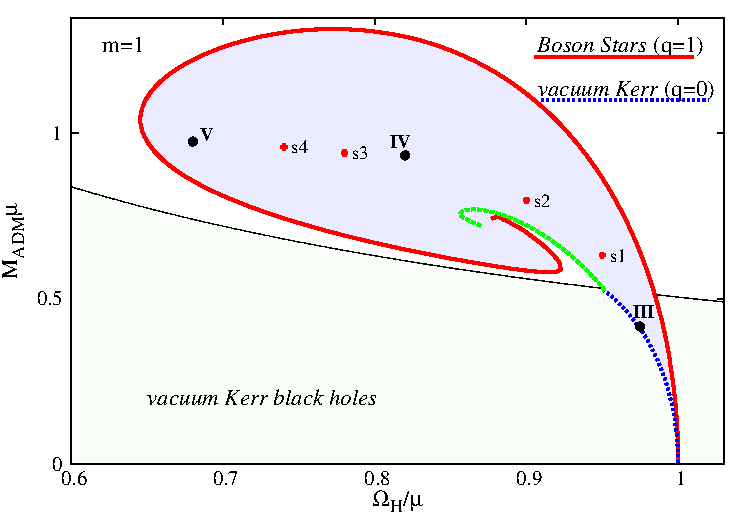
\includegraphics[scale=0.7]{figures/existence-eps-converted-to.pdf}
\caption{Domain of existence for KBHsSH in an ADM mass versus scalar
field frequency diagram. \tf{The figure has to be redone to label the 7 models used in this work.}}
\label{existence}
\end{figure}

\begin{figure*}
\centering
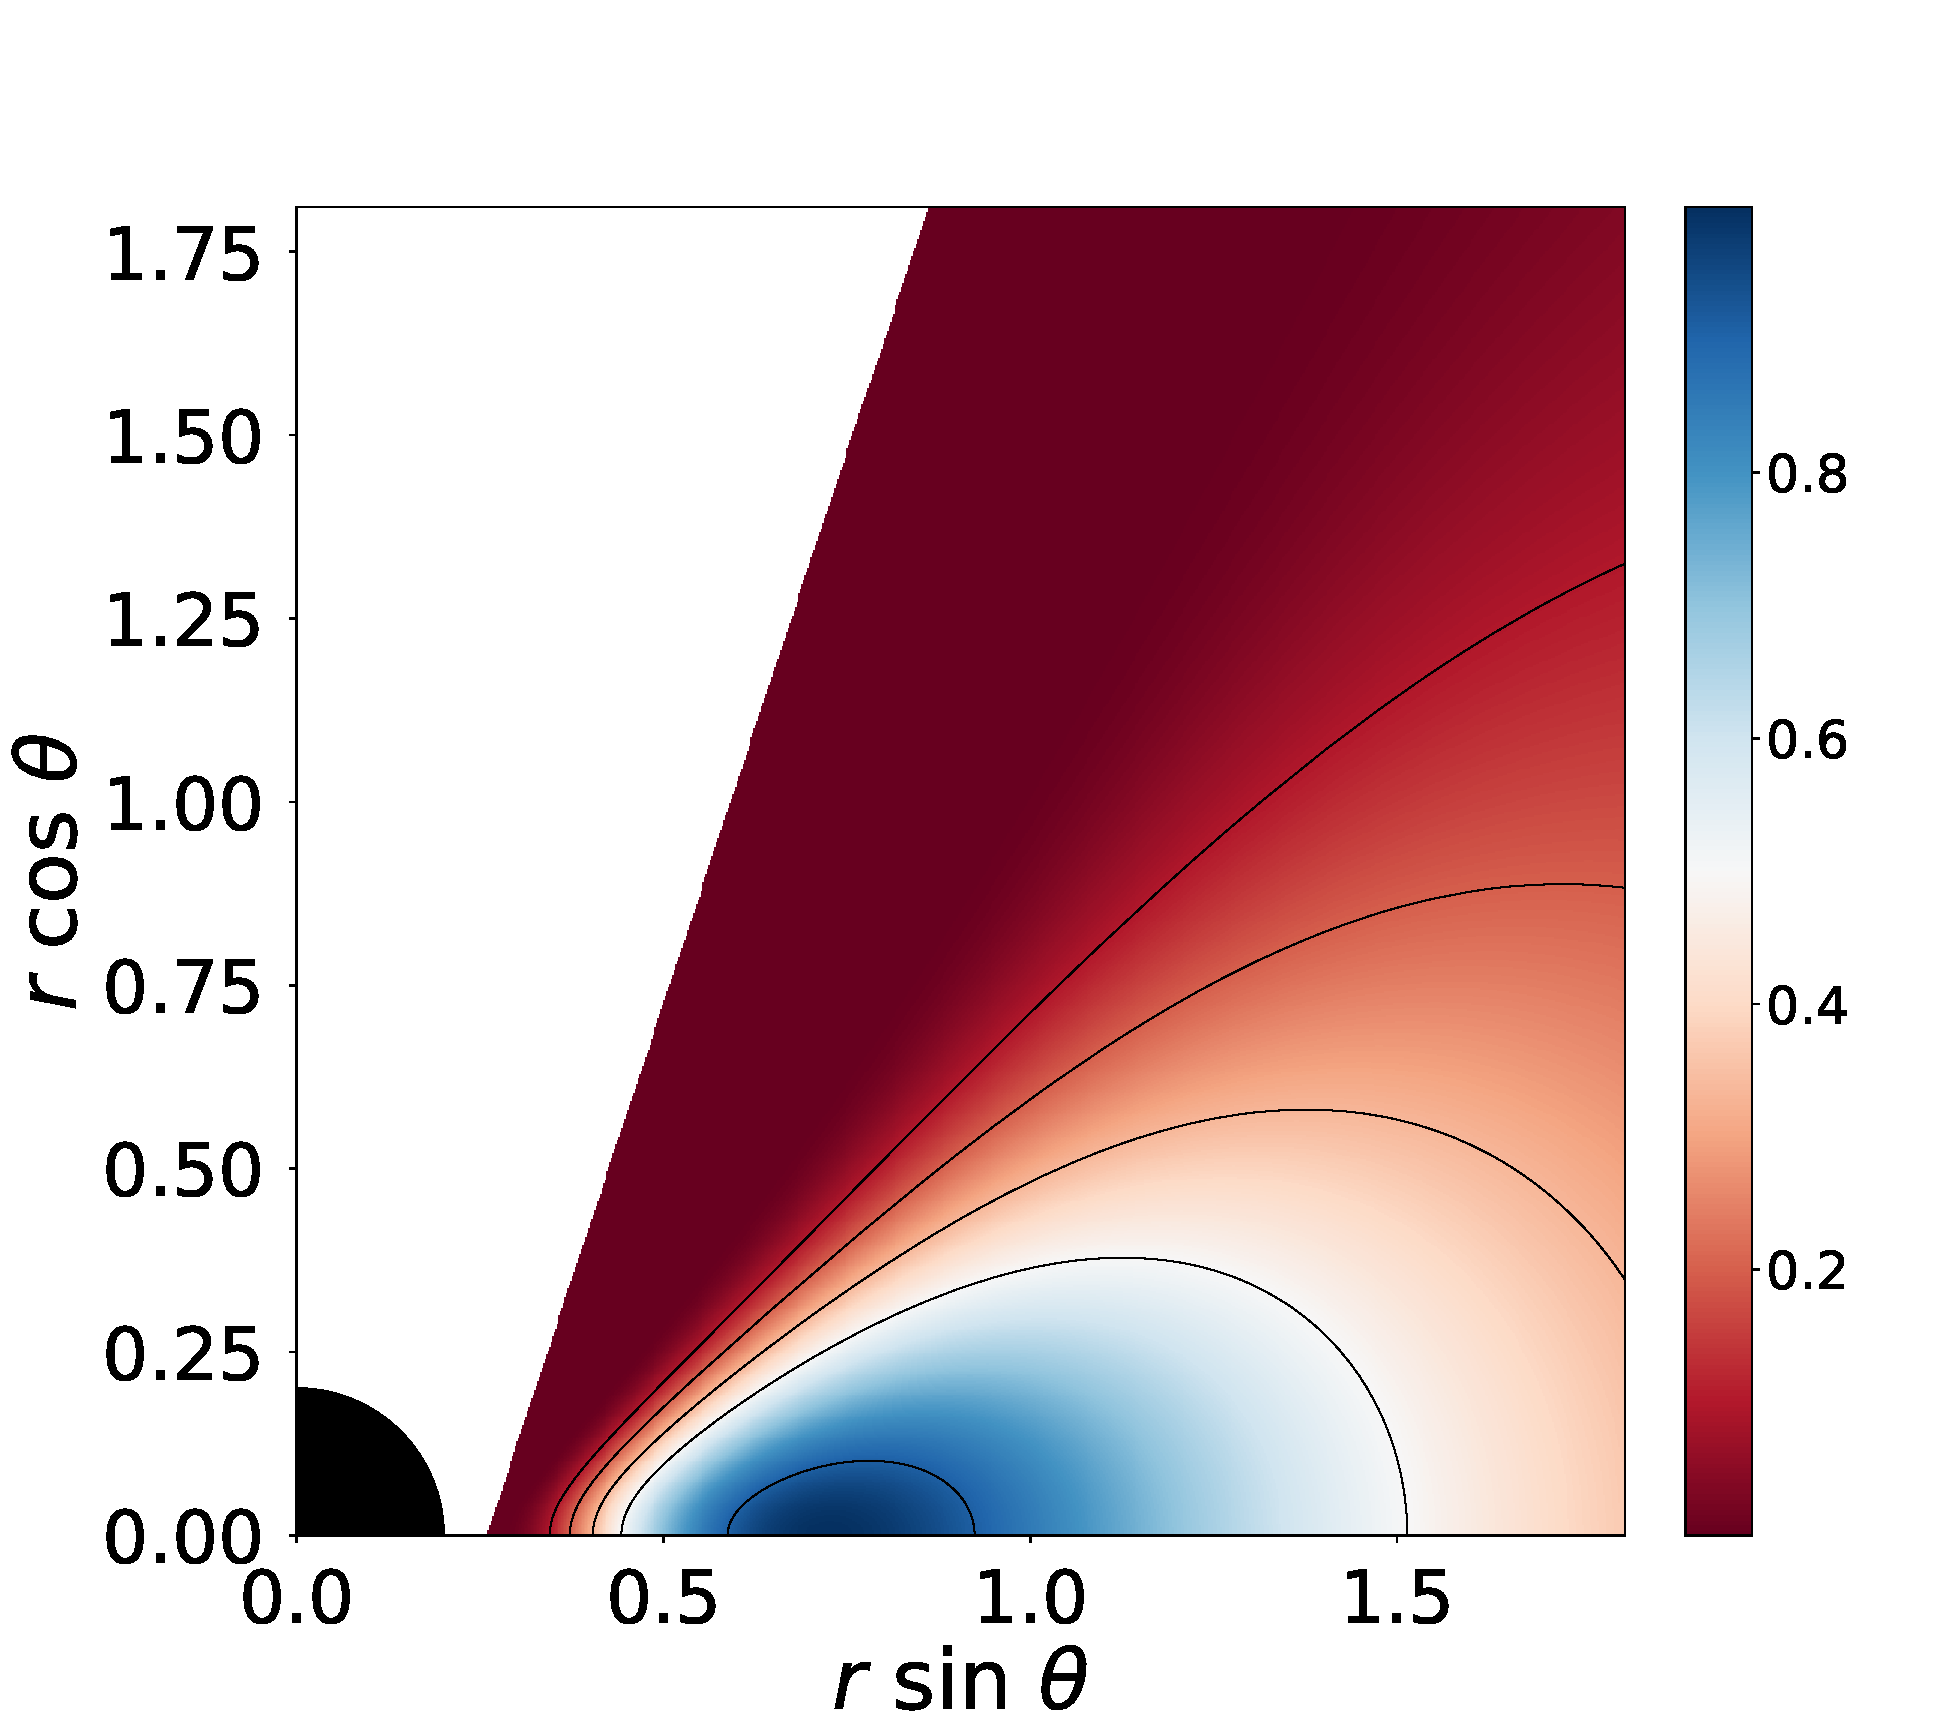
\includegraphics[scale=0.14]{figures/fig1_I_10.pdf}
\hspace{-0.3cm}
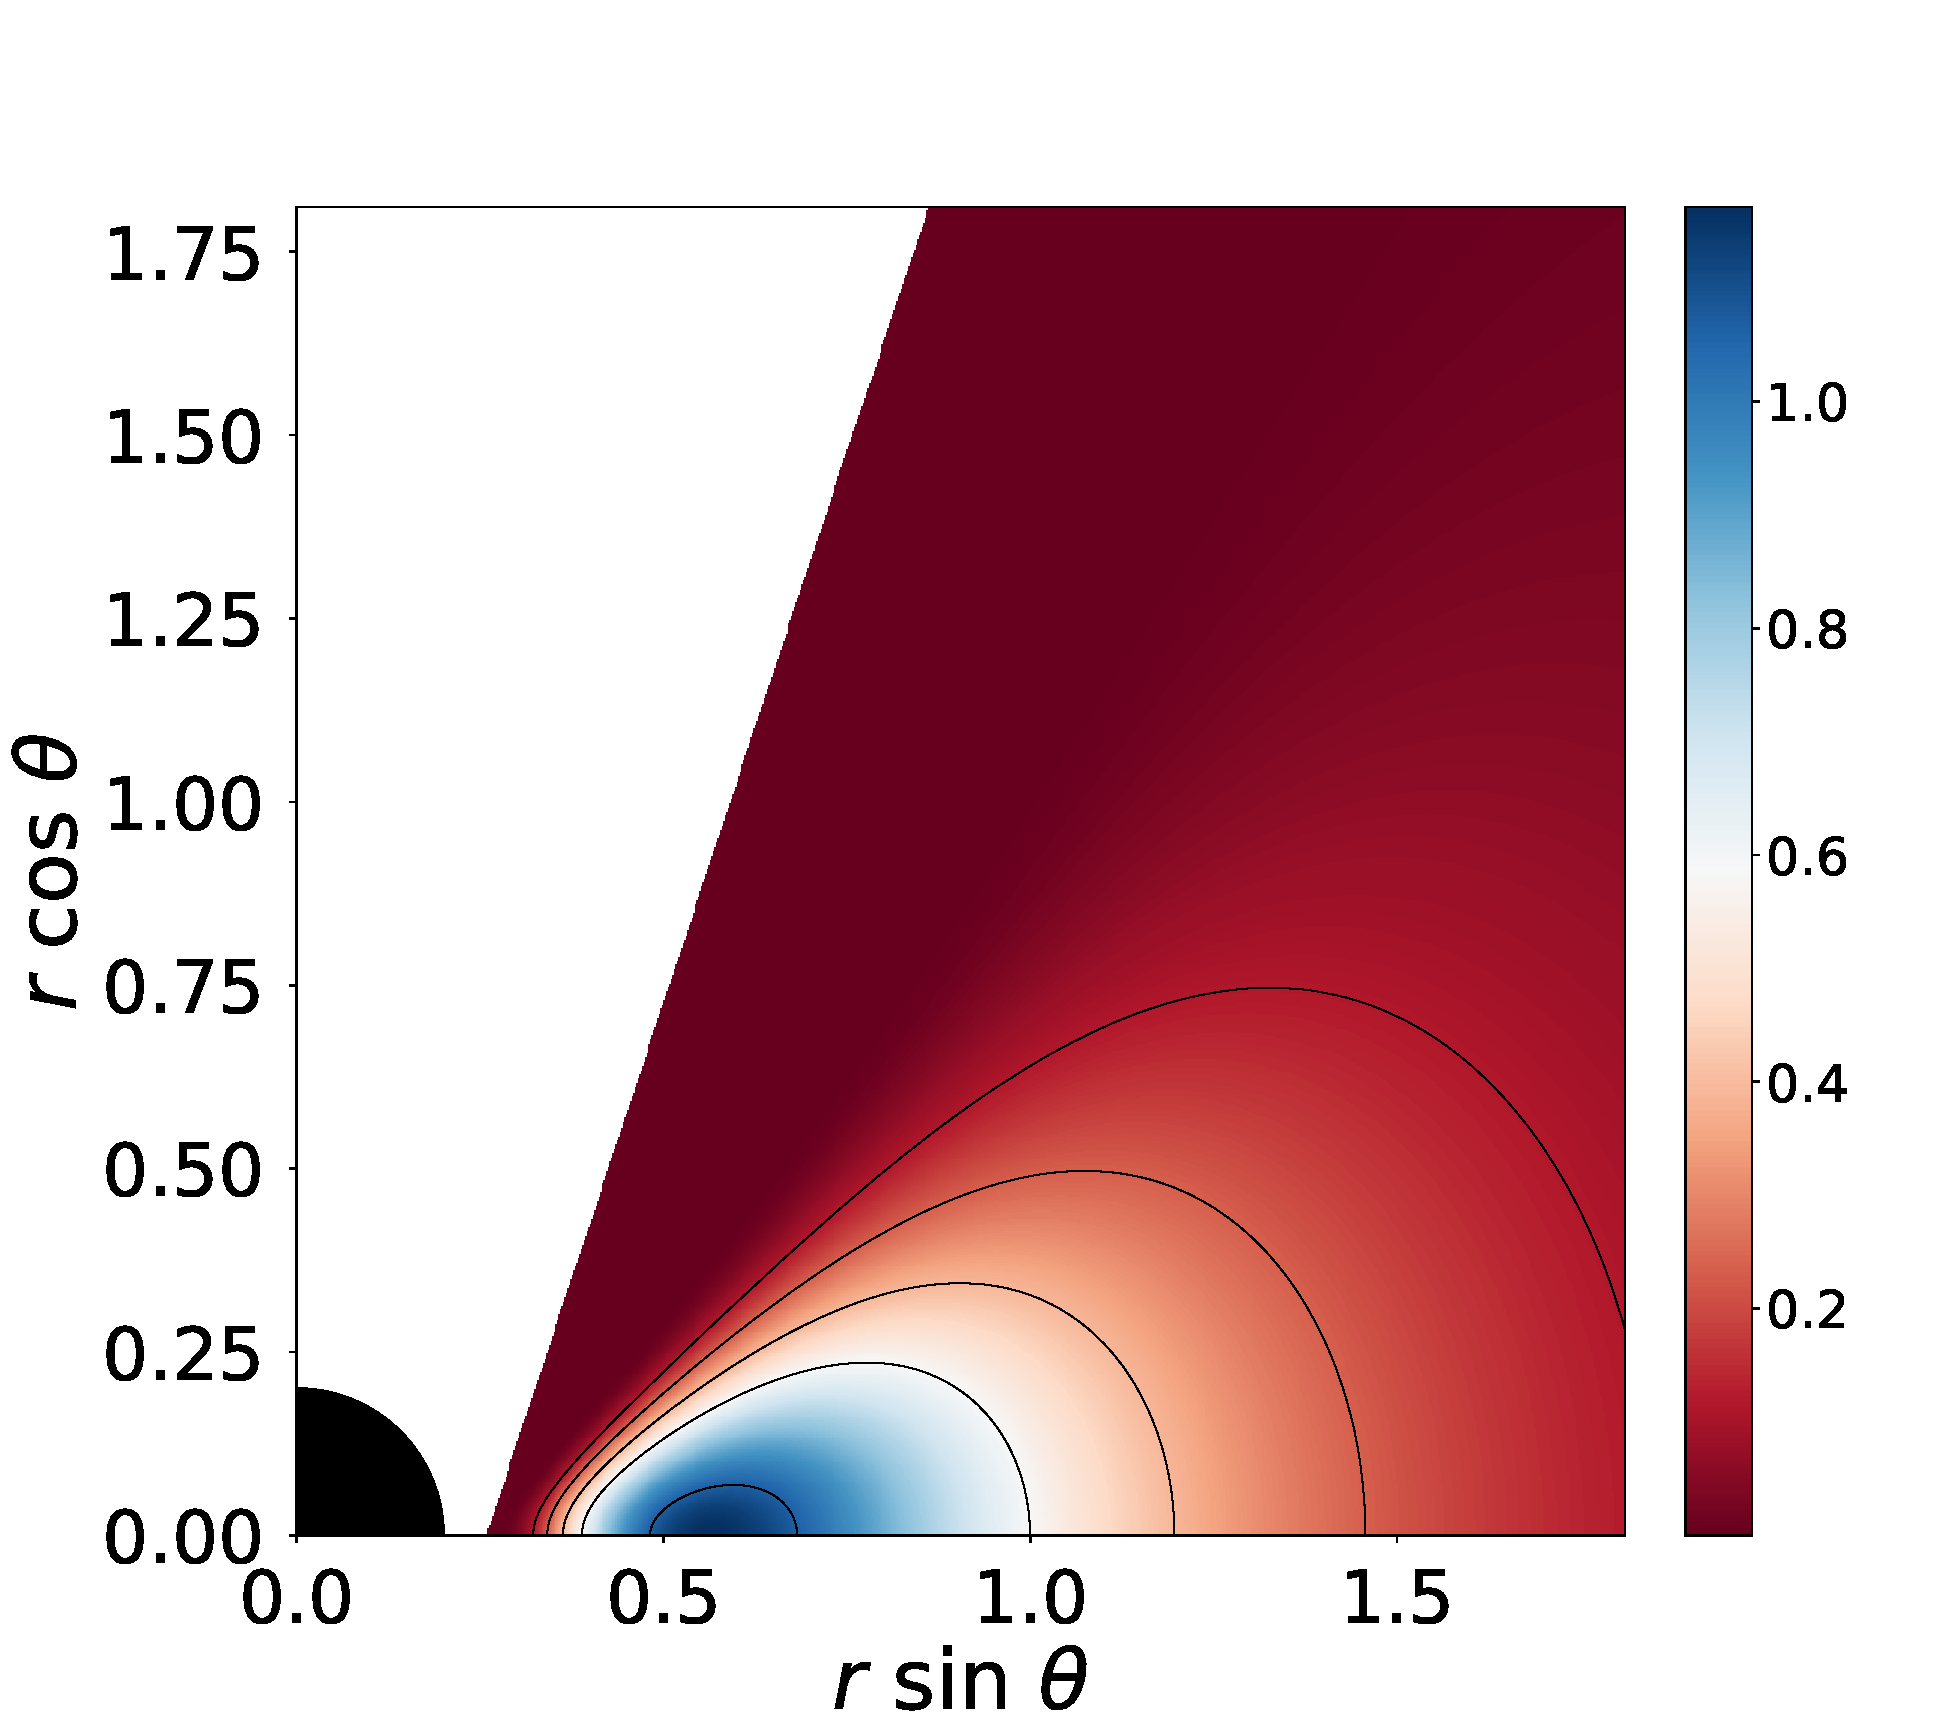
\includegraphics[scale=0.14]{figures/fig1_I_1.pdf}
\hspace{-0.2cm}
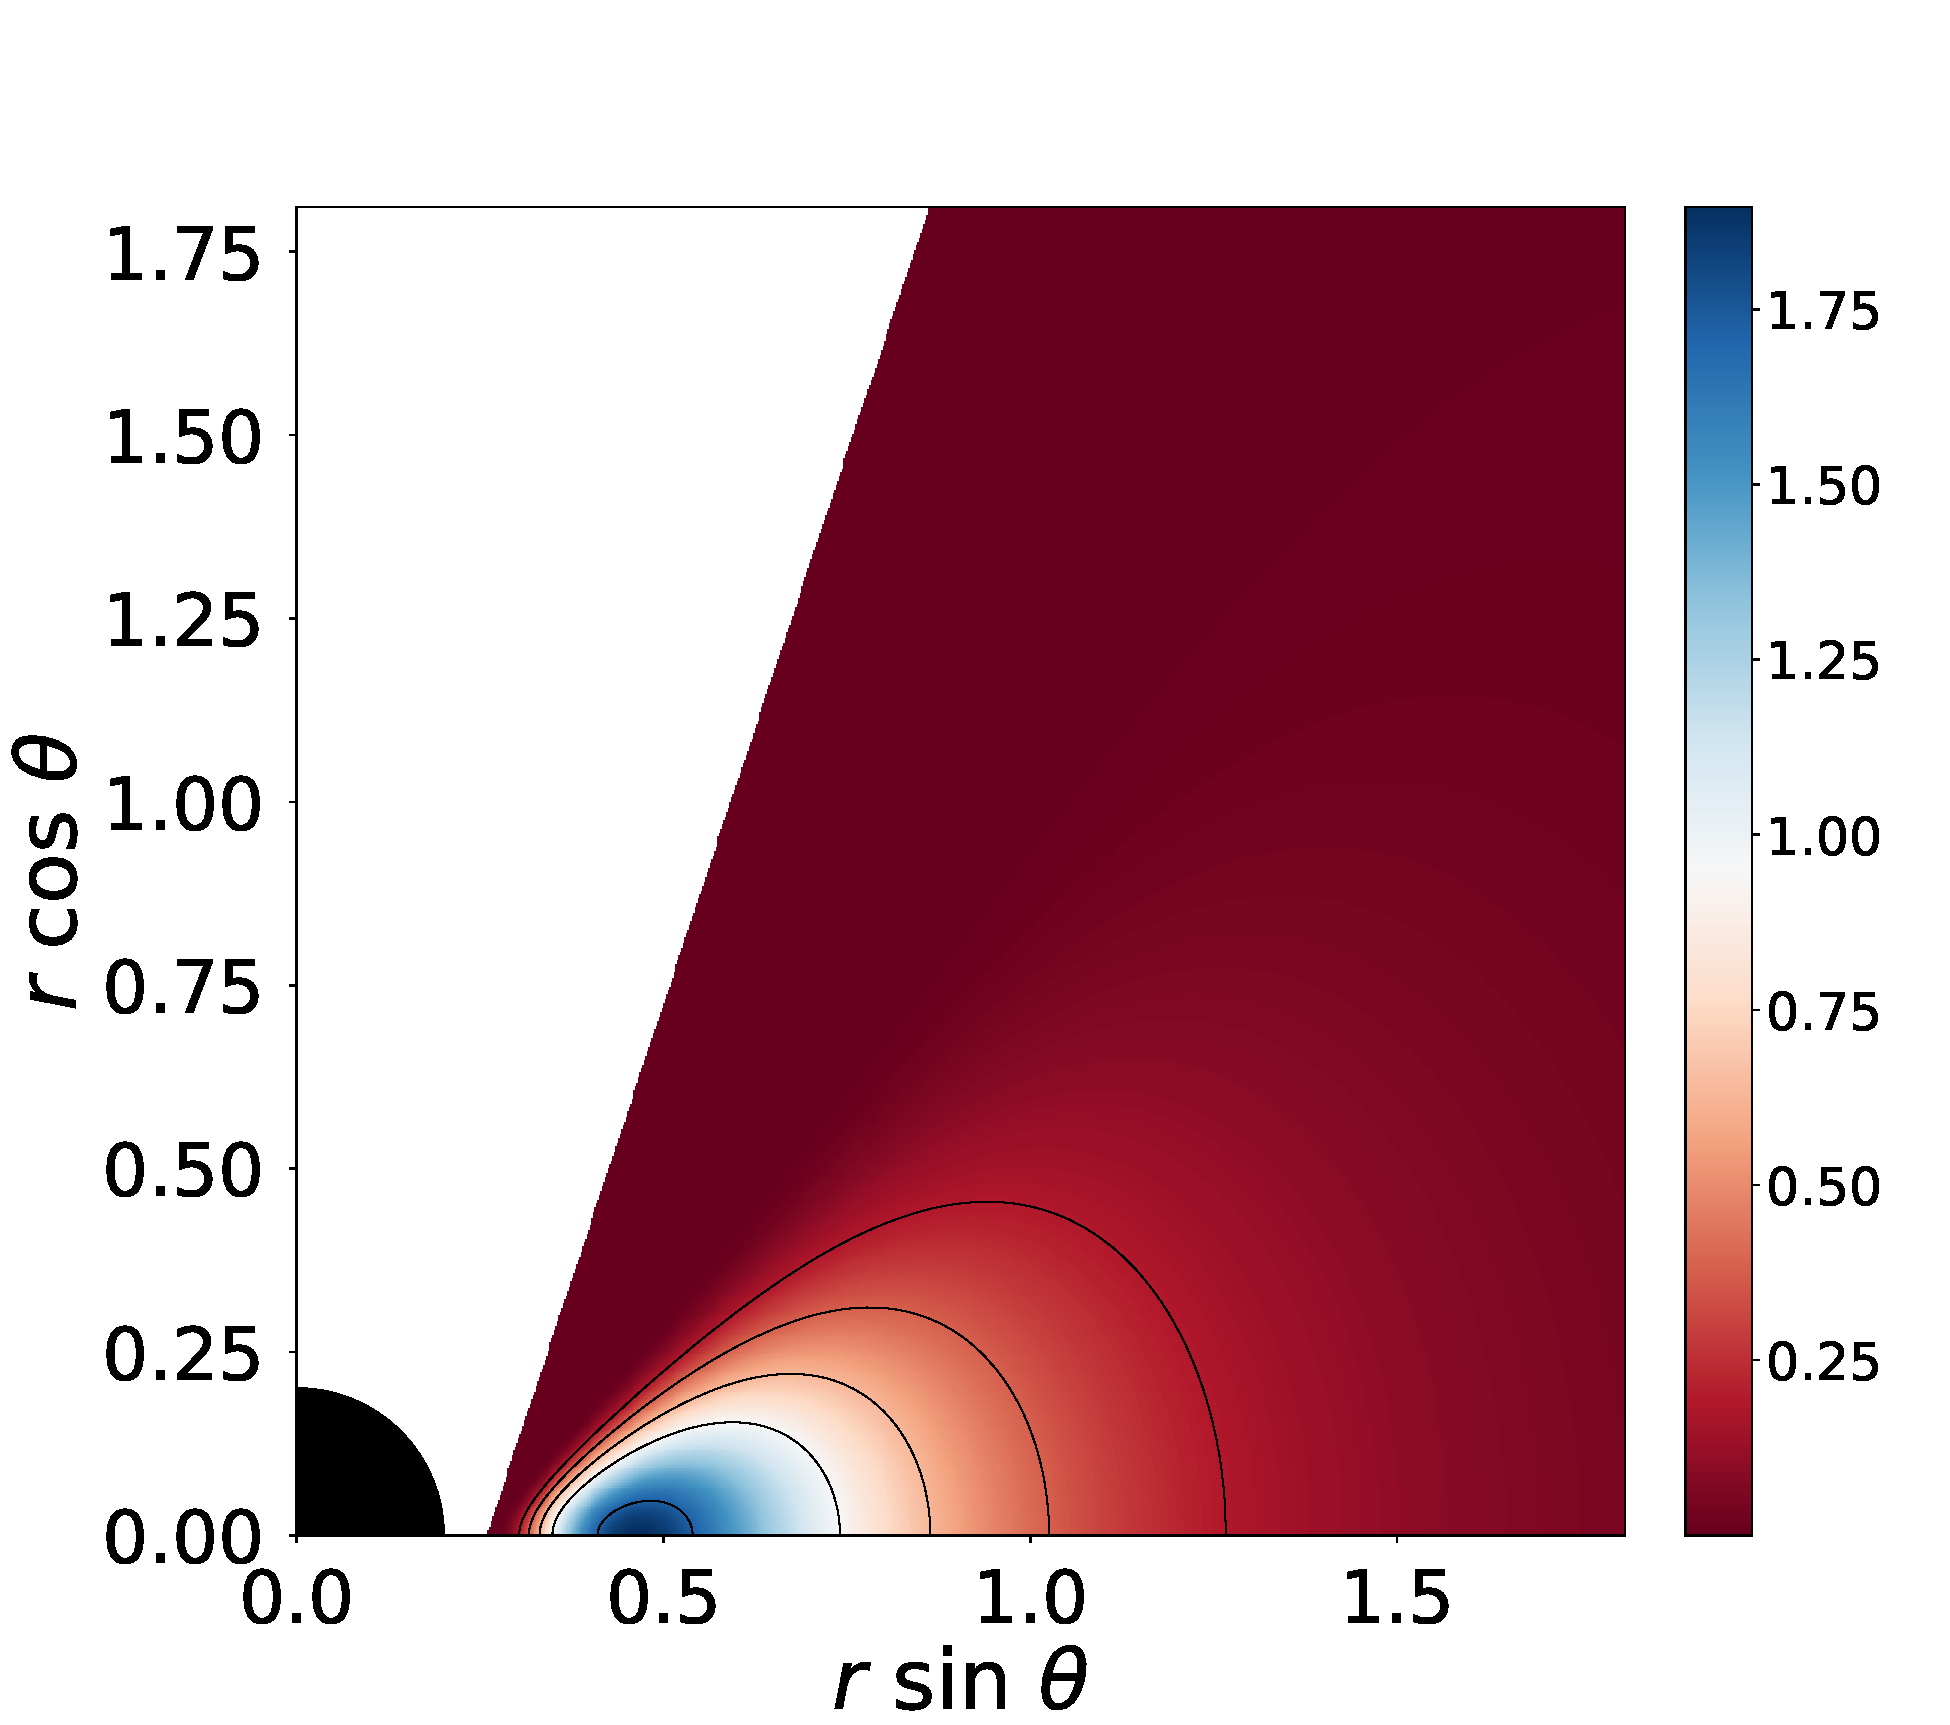
\includegraphics[scale=0.14]{figures/fig1_I__10.pdf}
\\
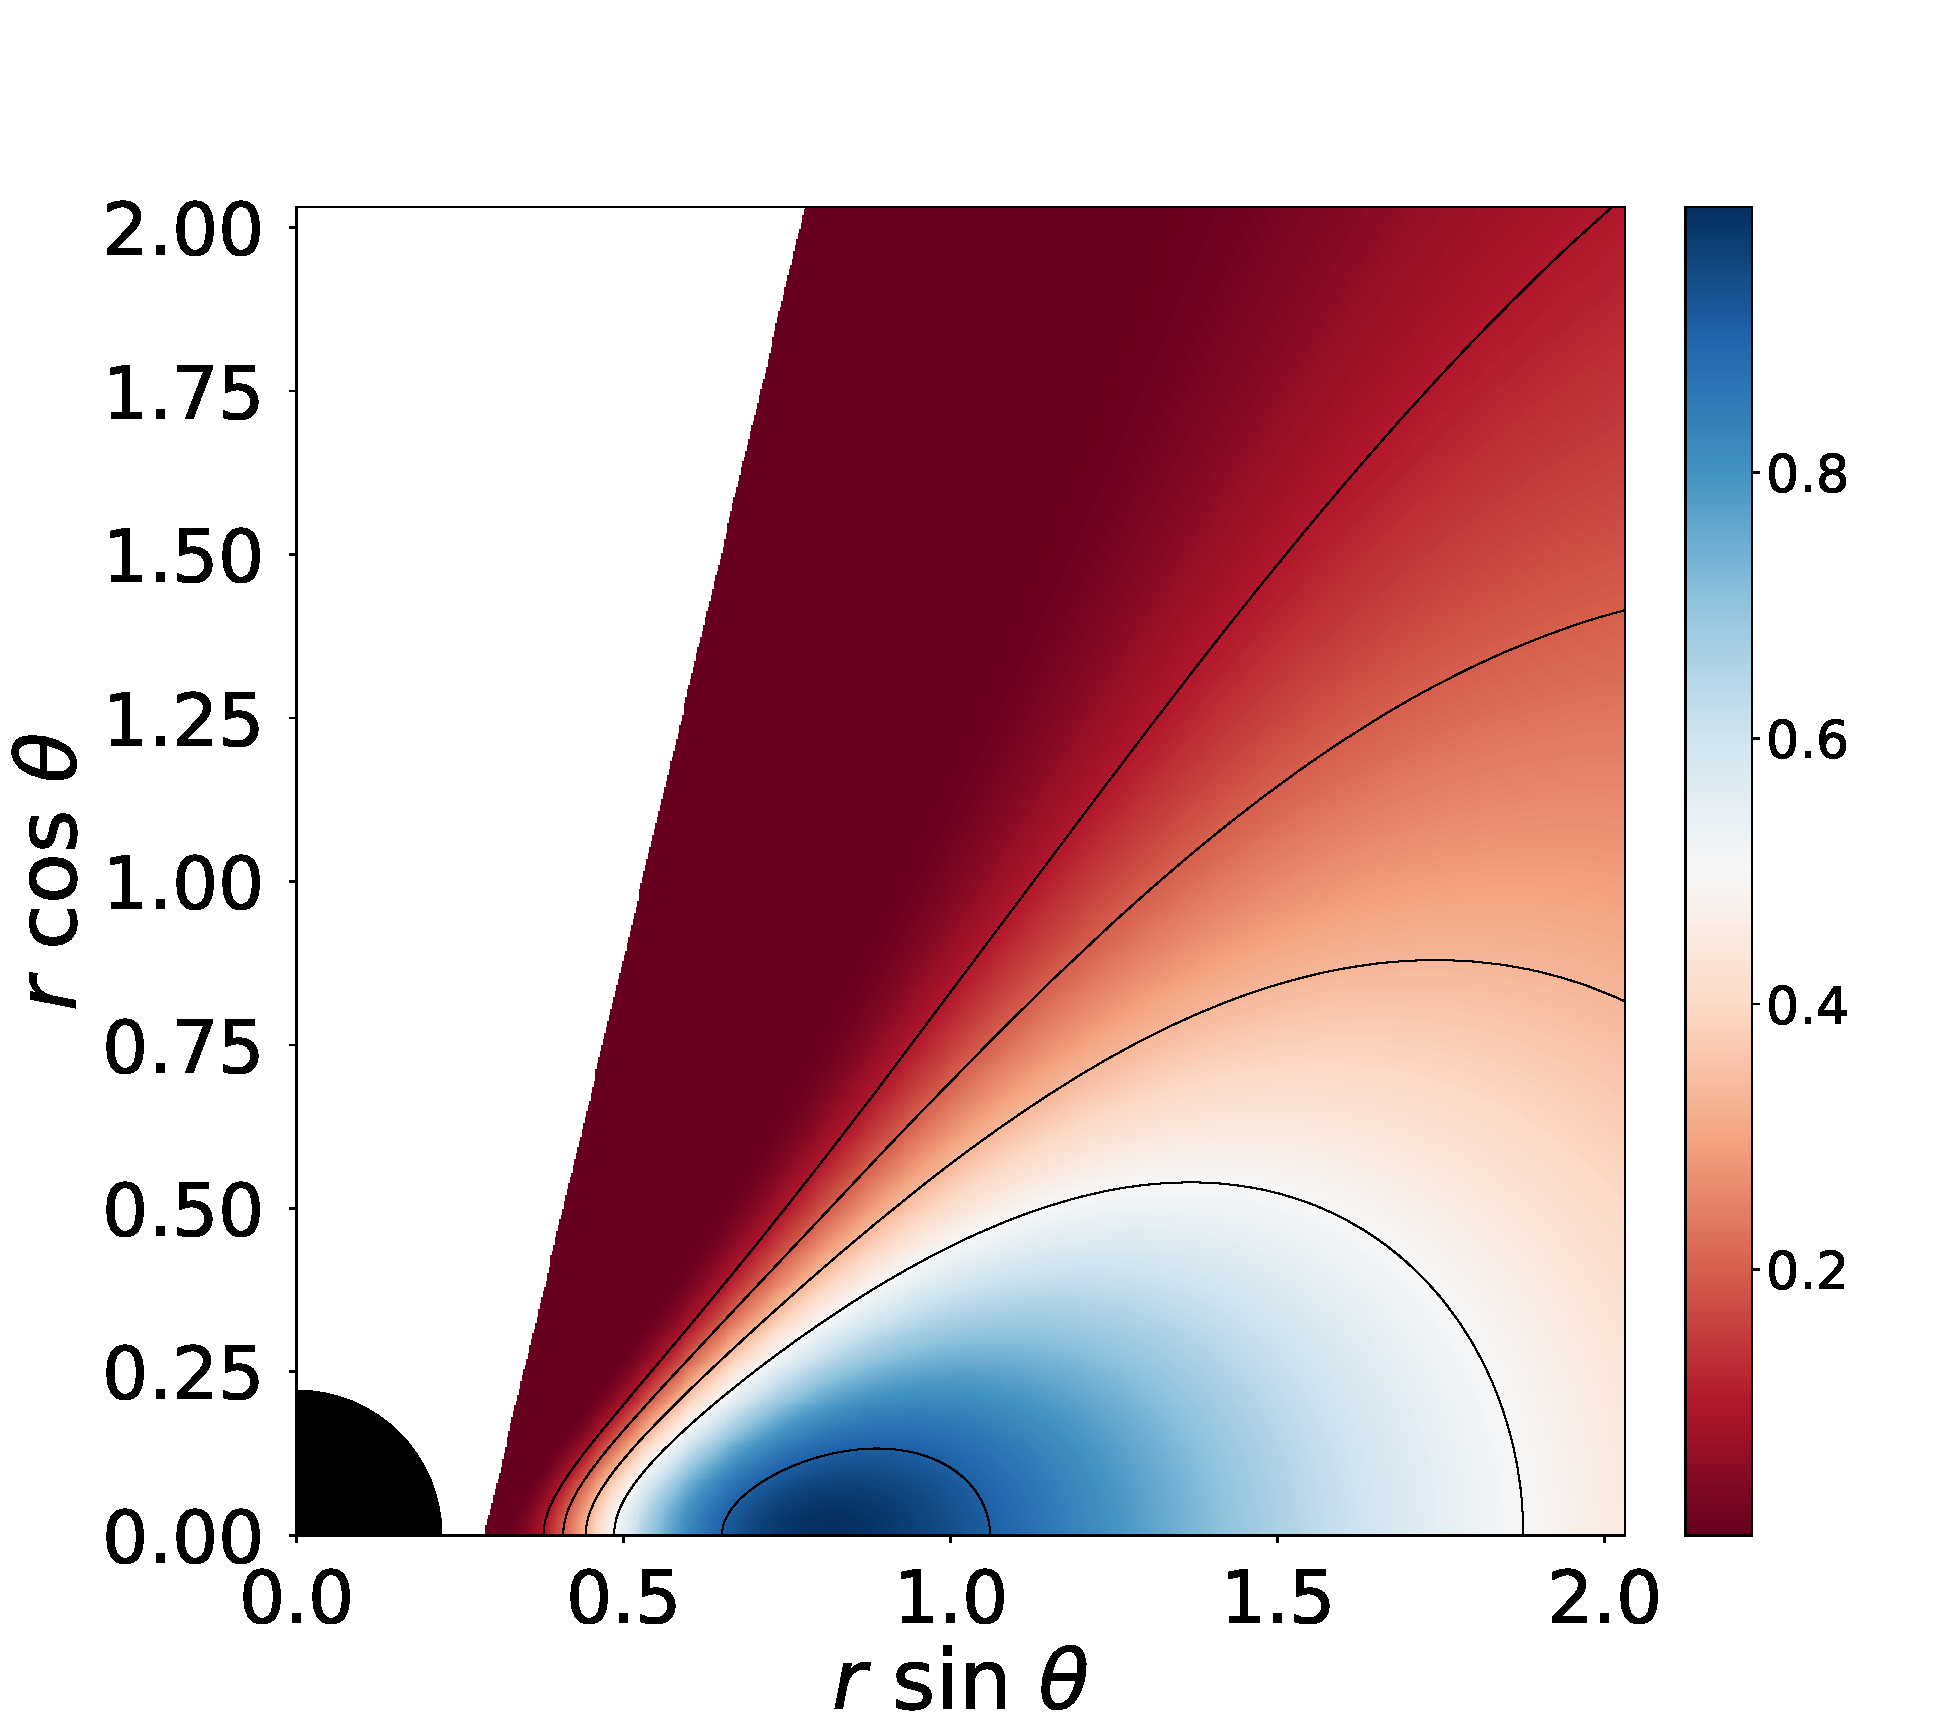
\includegraphics[scale=0.14]{figures/fig1_II_10.pdf}
\hspace{-0.3cm}
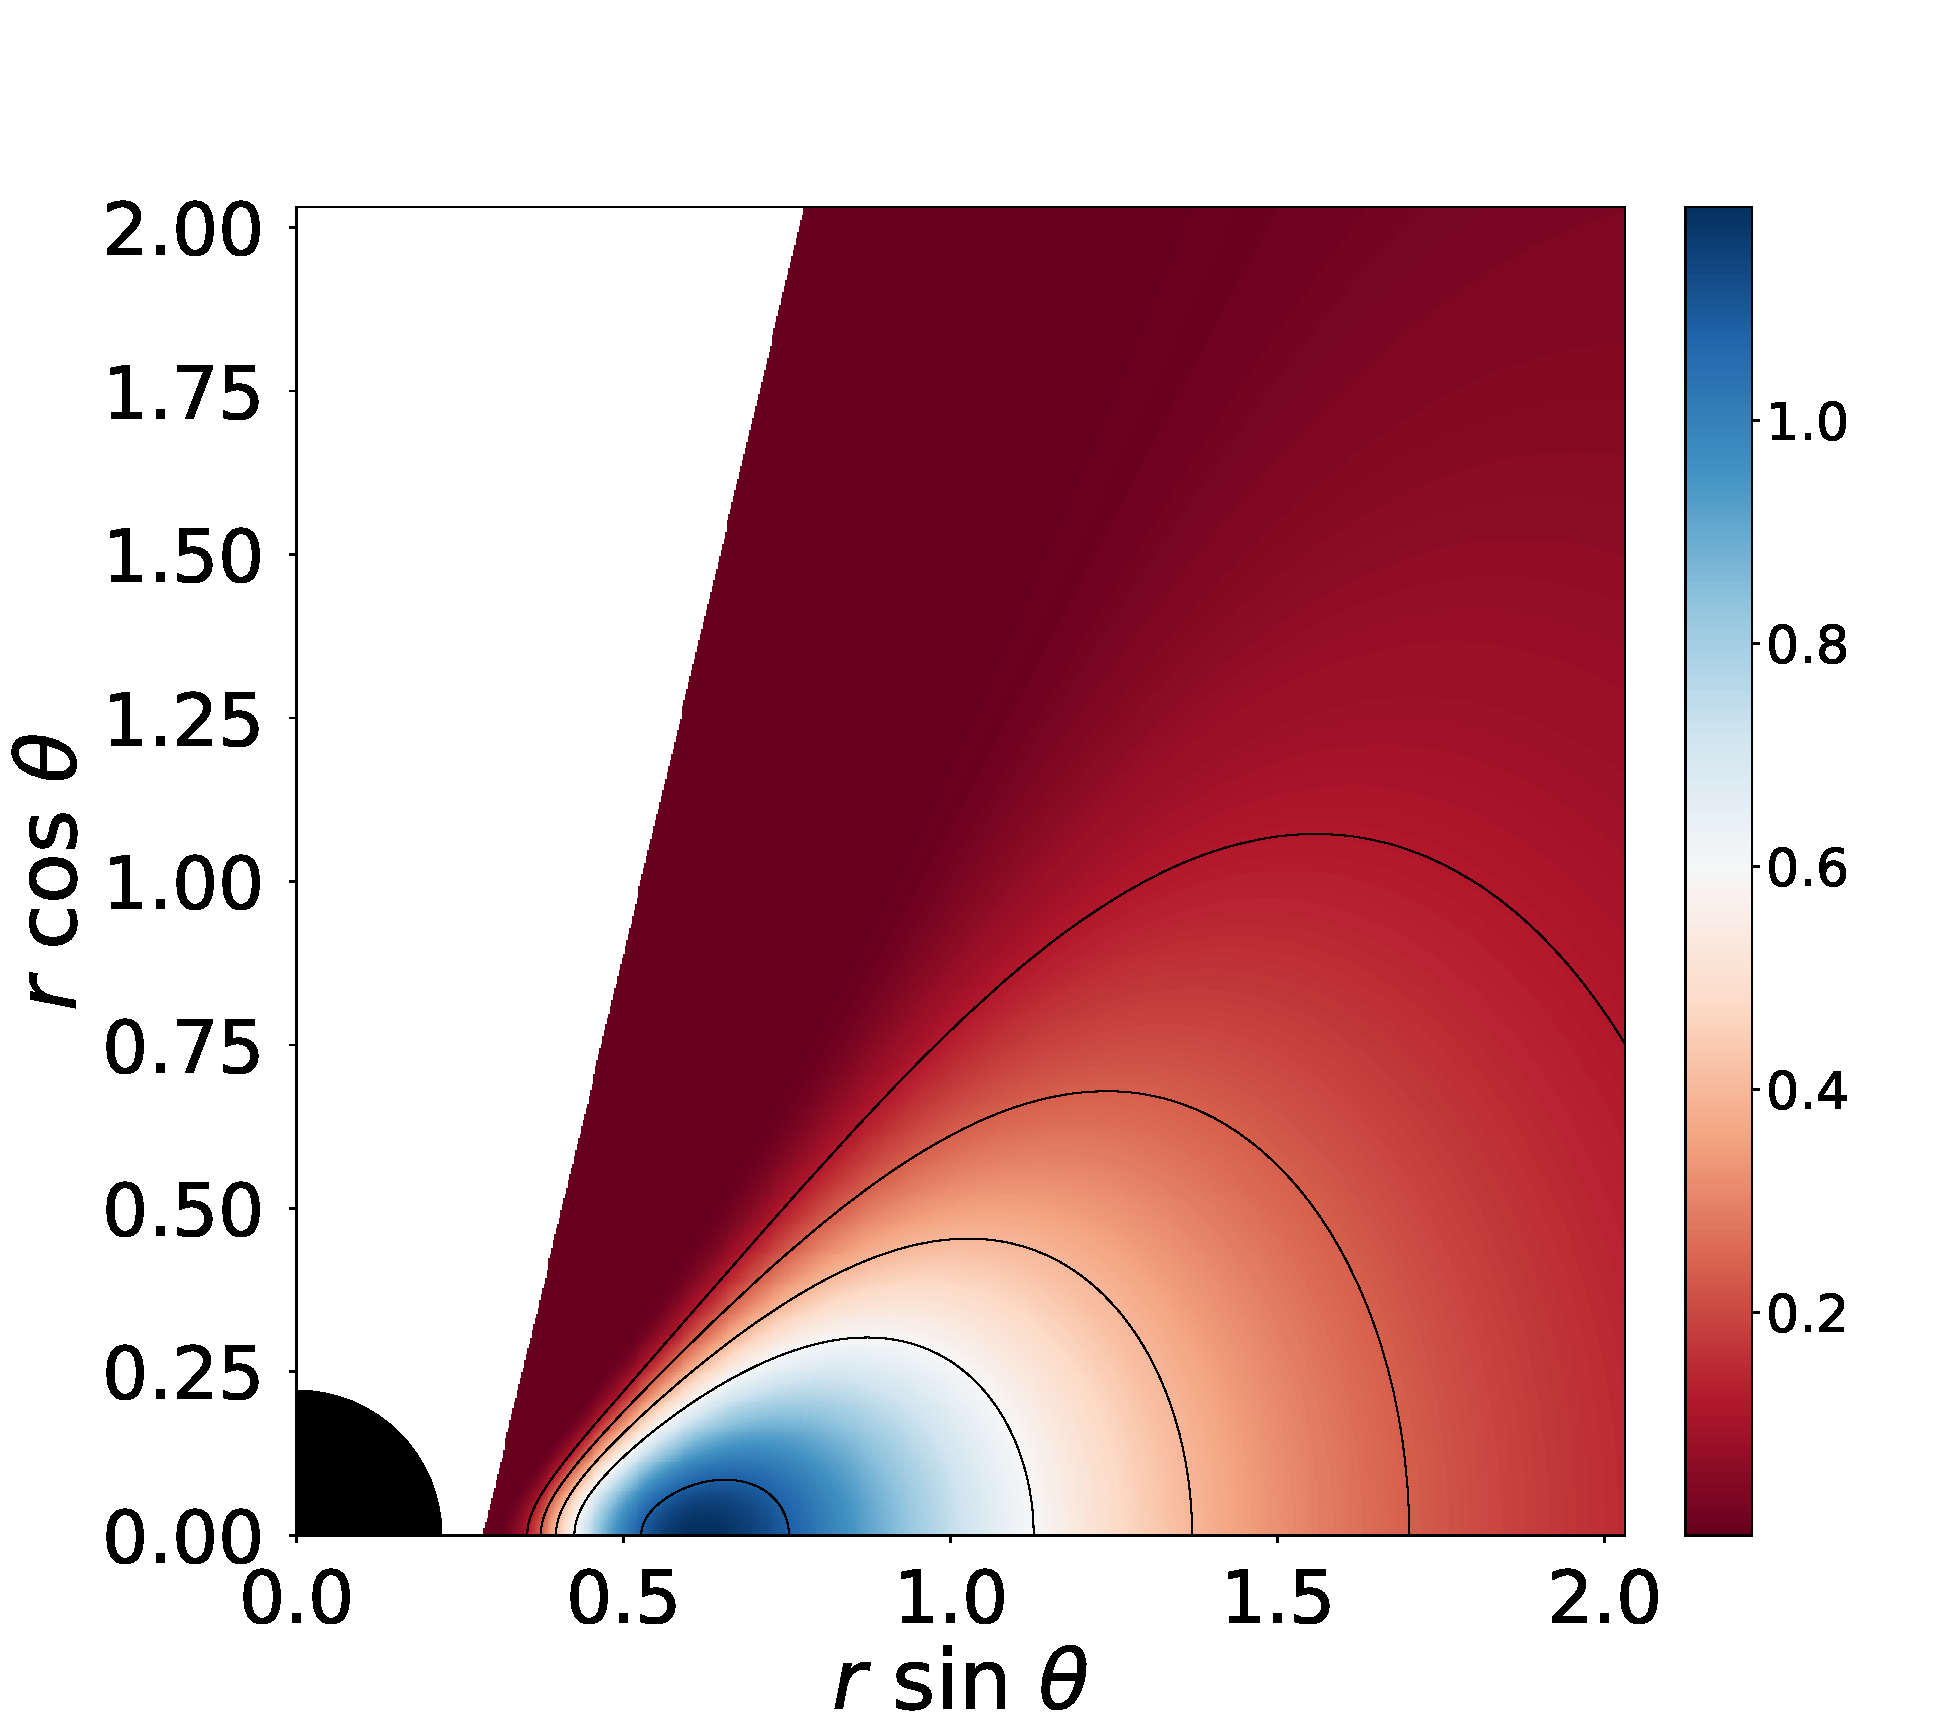
\includegraphics[scale=0.14]{figures/fig1_II_1.pdf}
\hspace{-0.2cm}
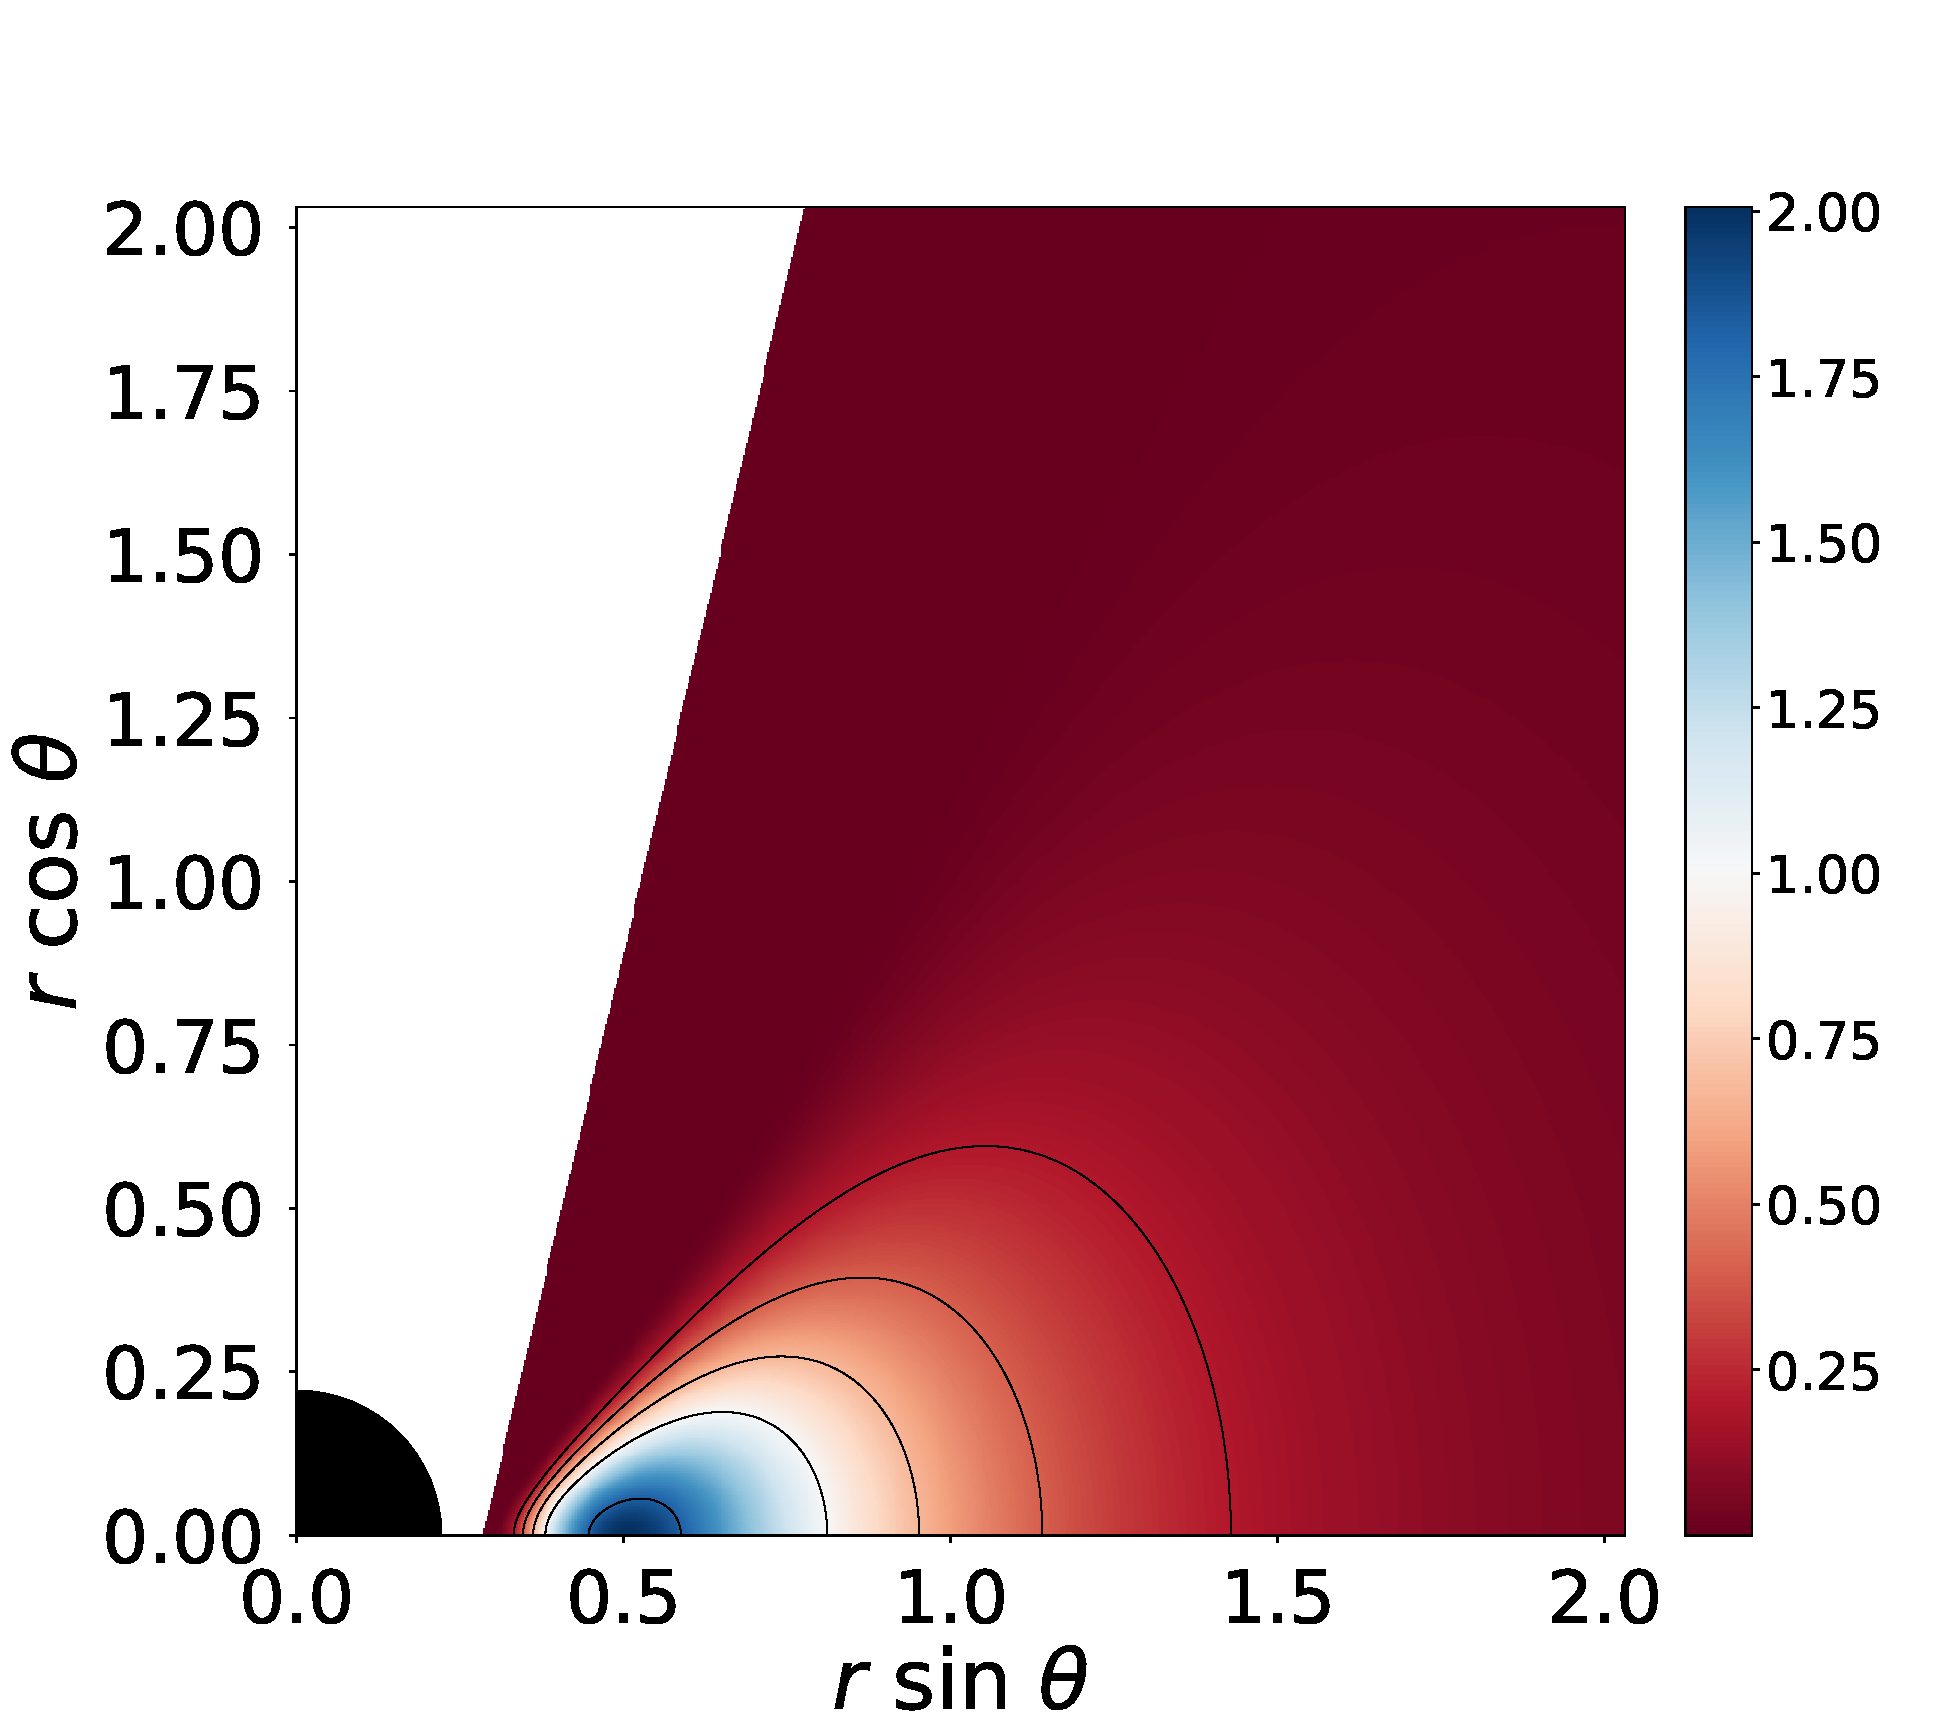
\includegraphics[scale=0.14]{figures/fig1_II__10.pdf}
\\
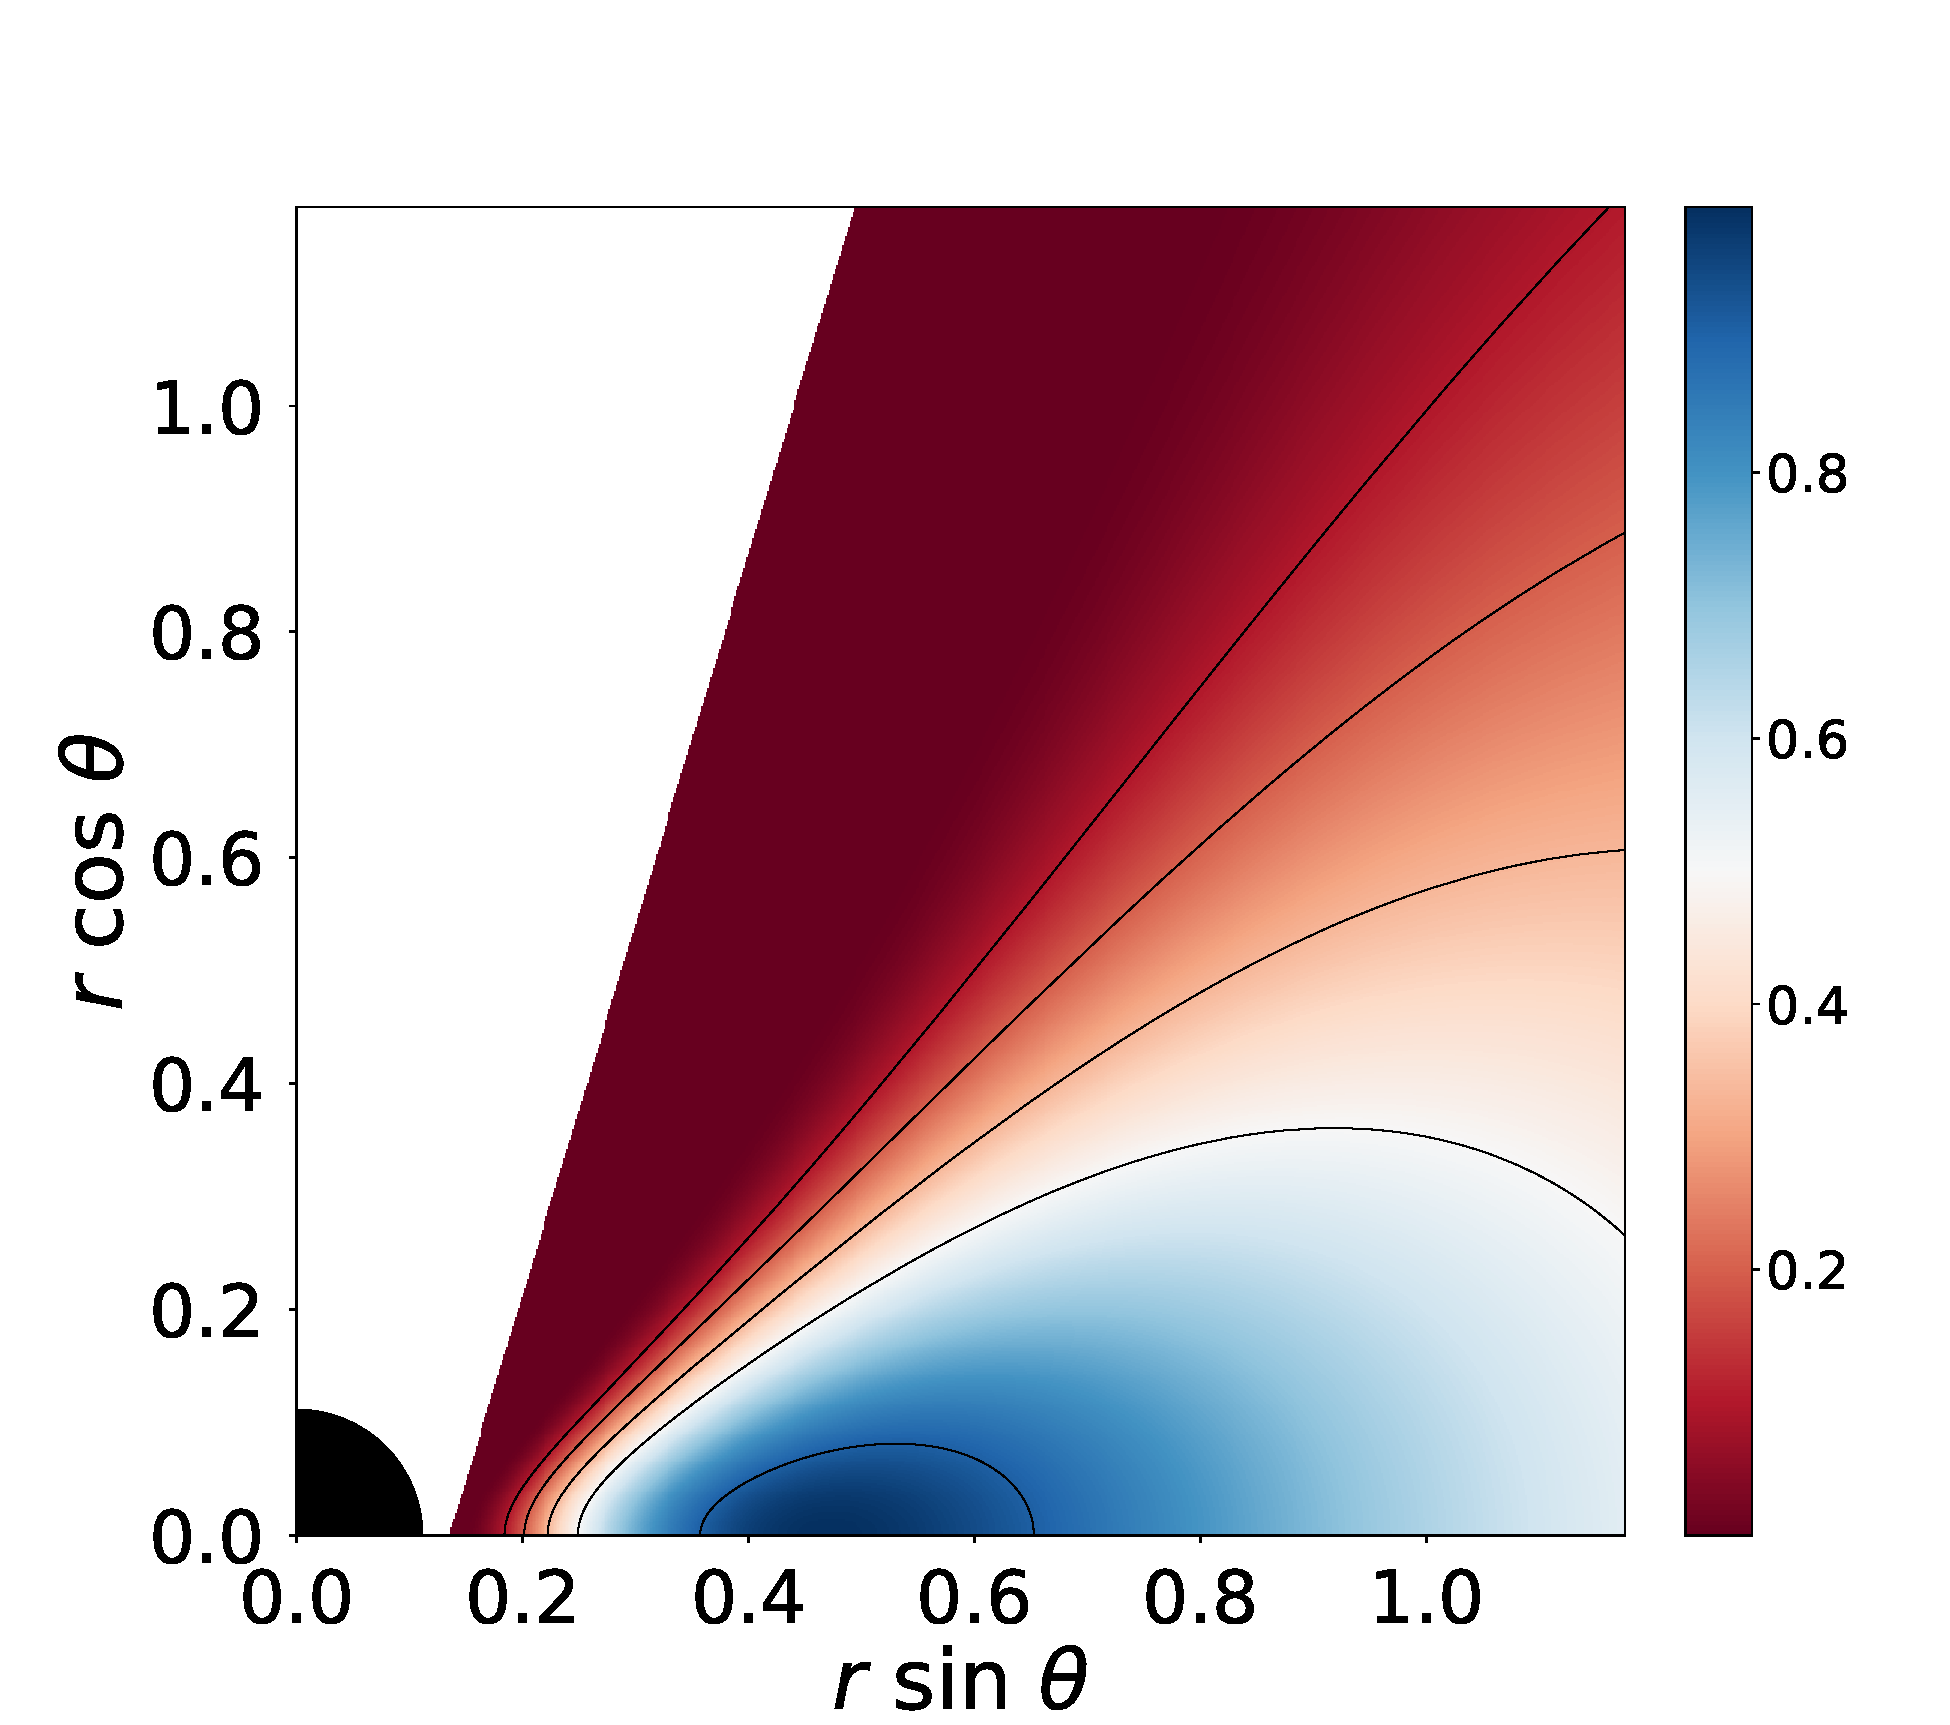
\includegraphics[scale=0.14]{figures/fig1_III_10.pdf}
\hspace{-0.3cm}
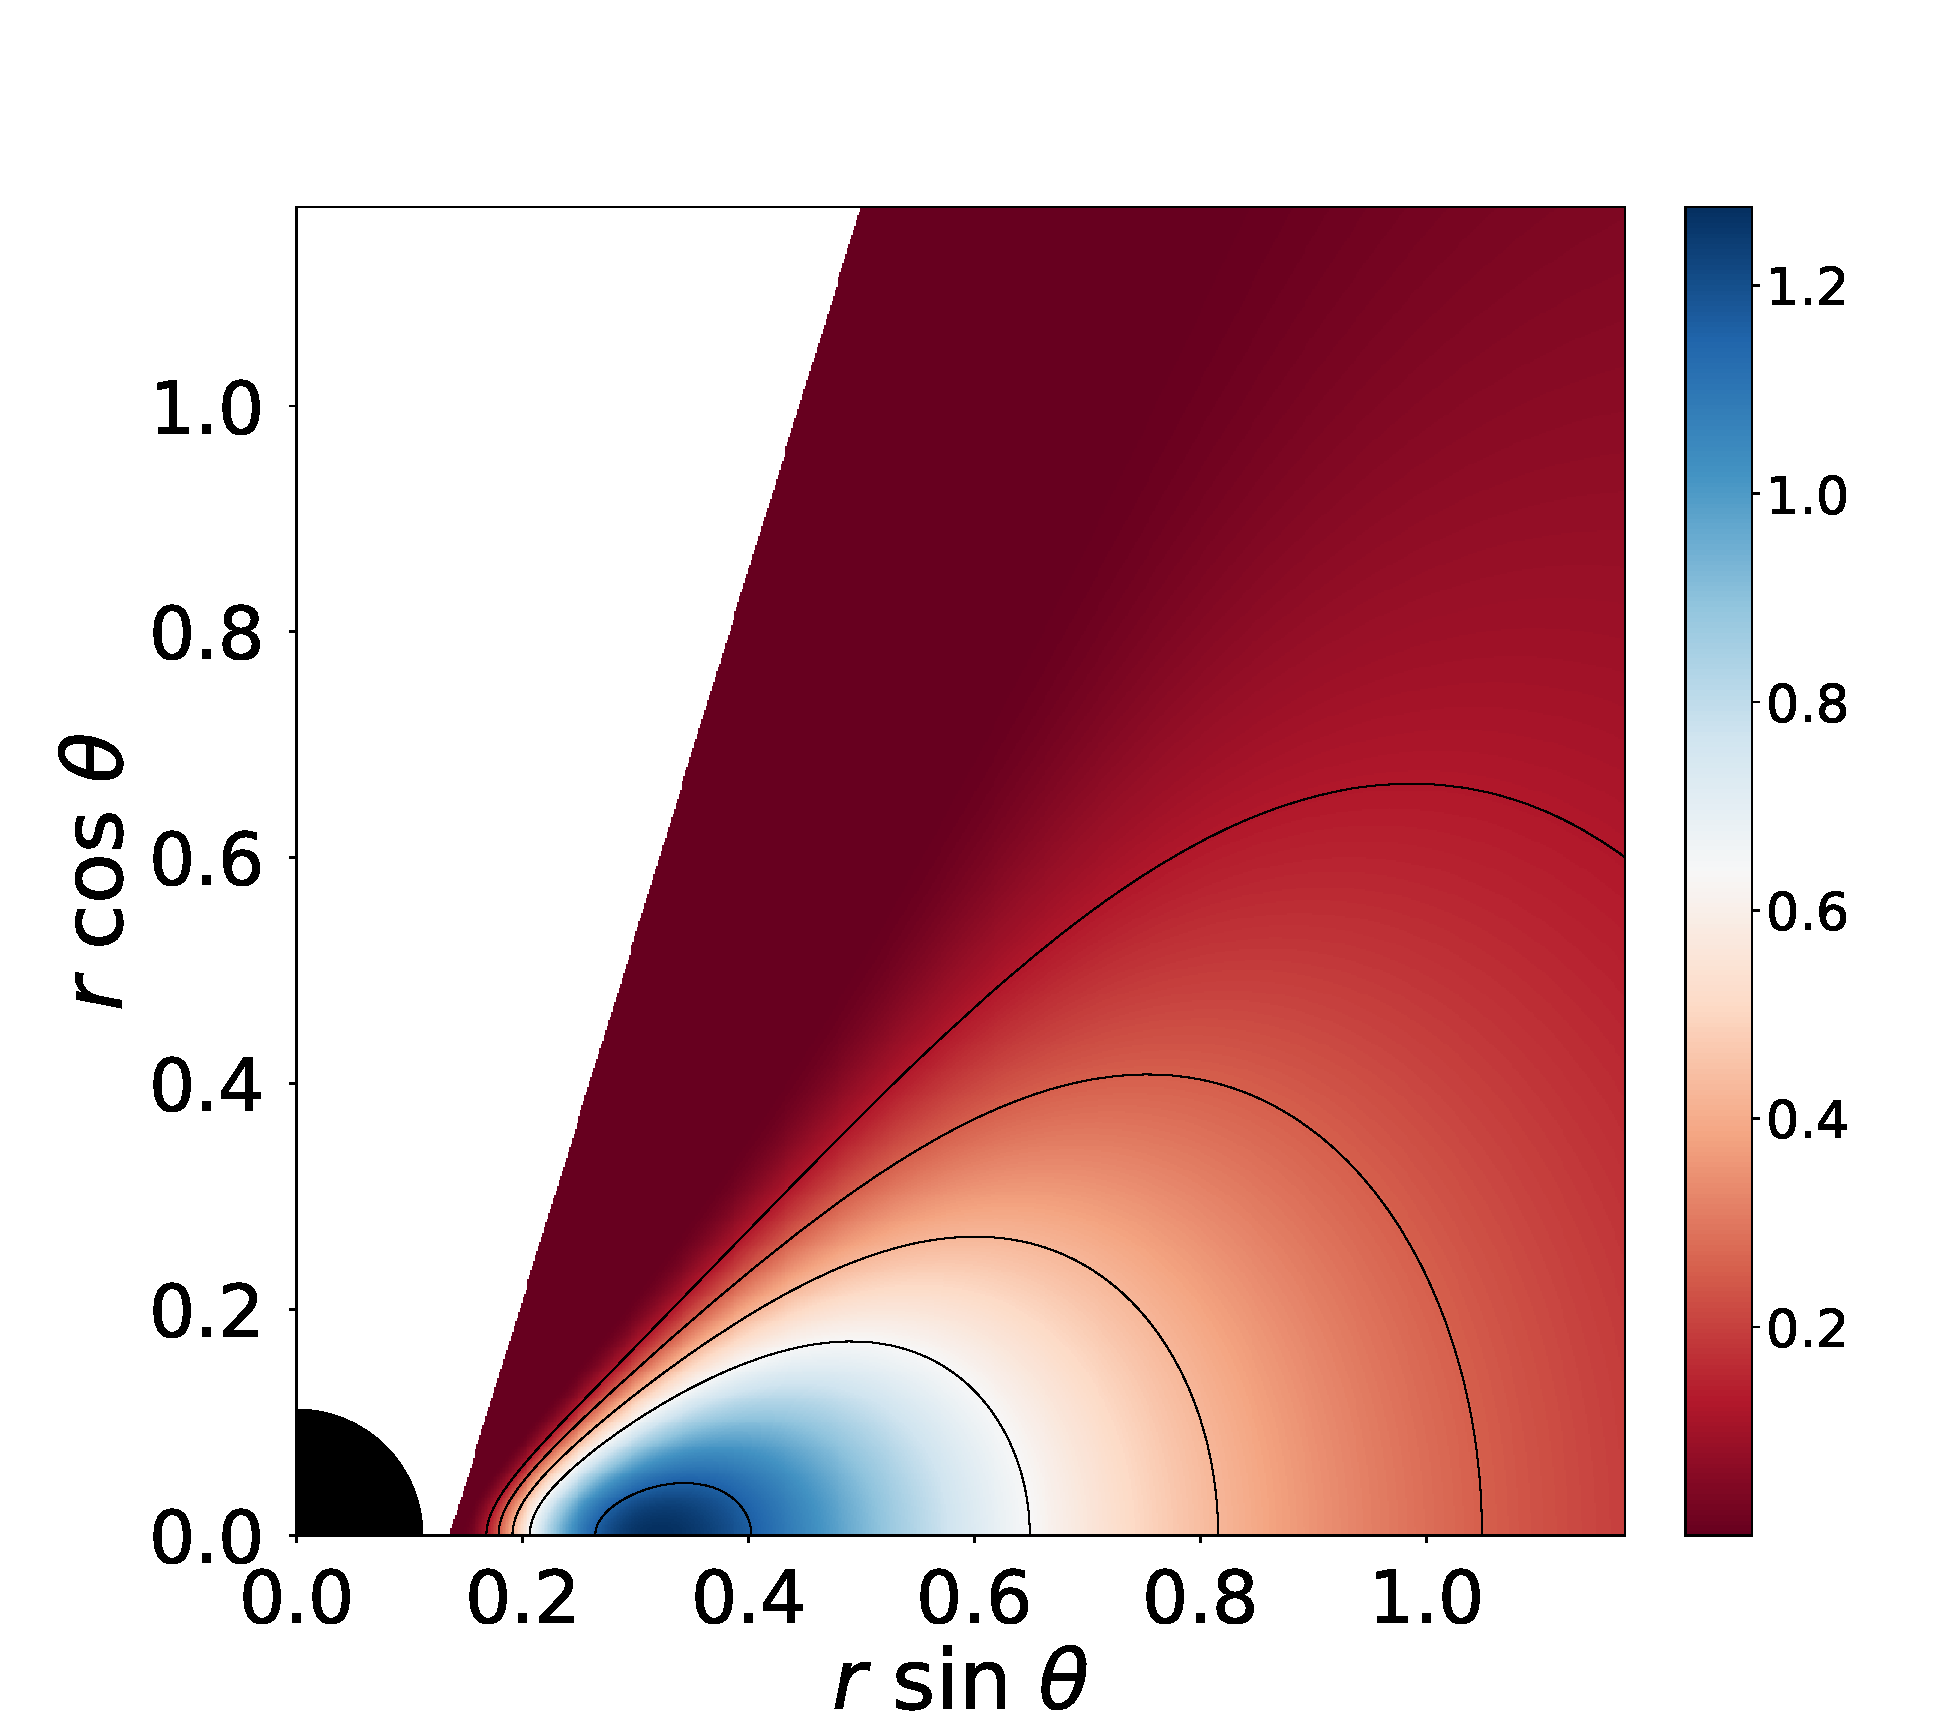
\includegraphics[scale=0.14]{figures/fig1_III_1.pdf}
\hspace{-0.2cm}
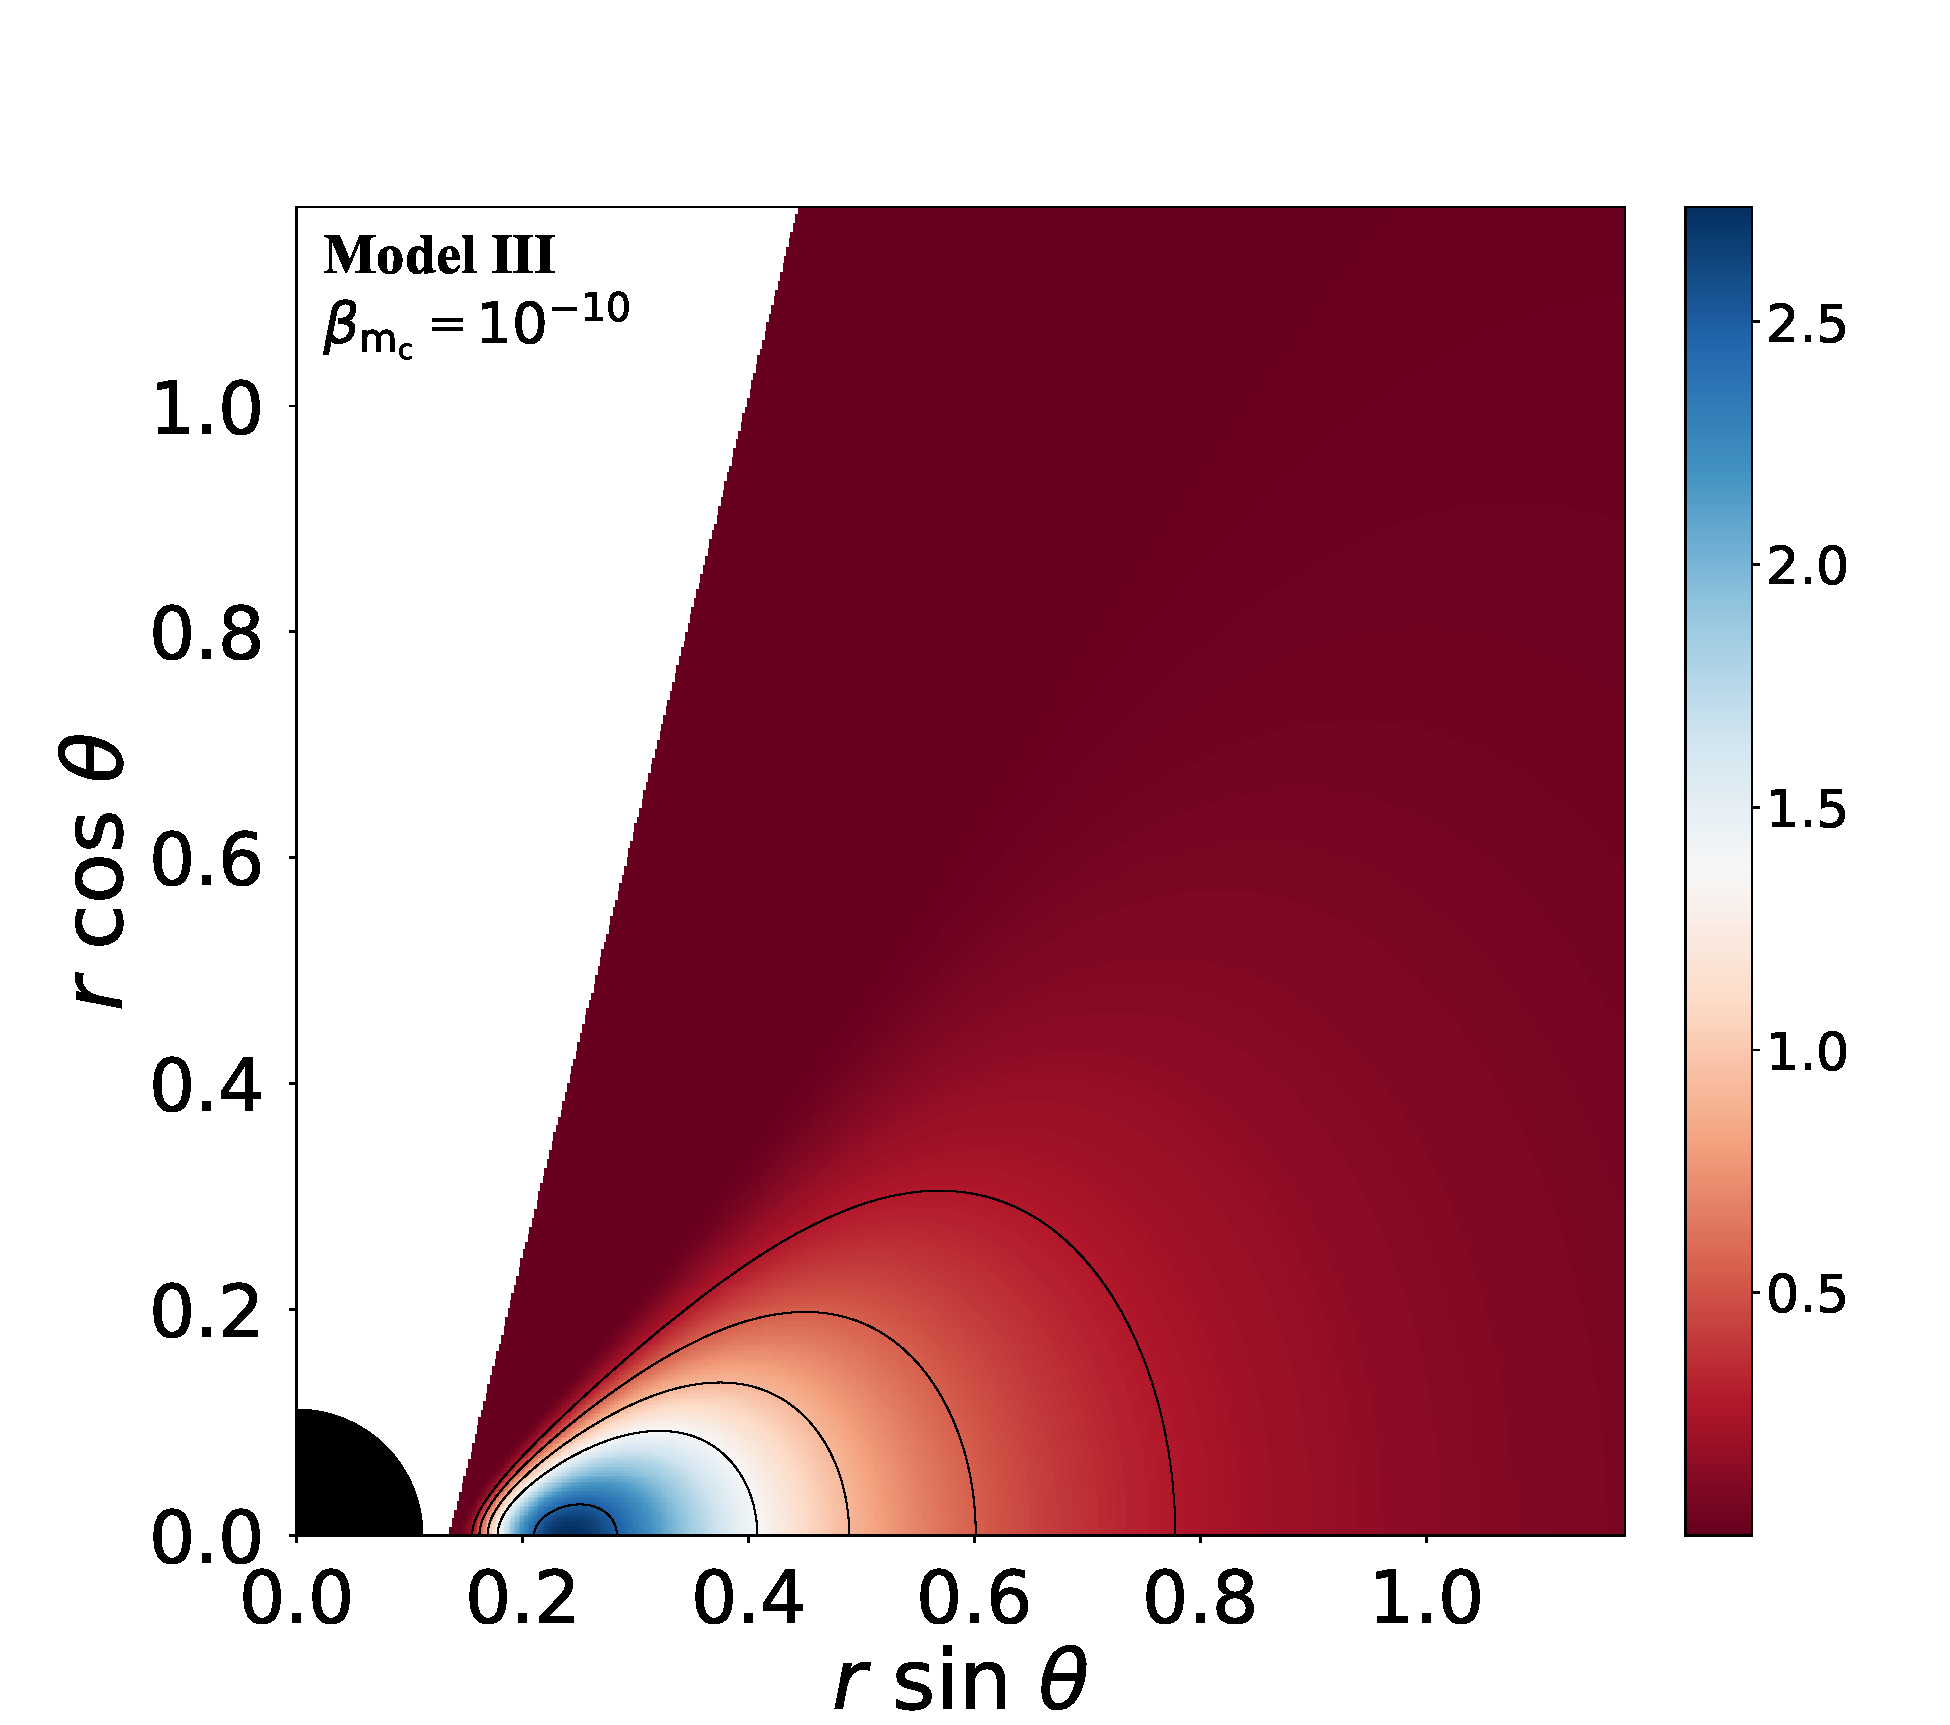
\includegraphics[scale=0.14]{figures/fig1_III__10.pdf}
\\
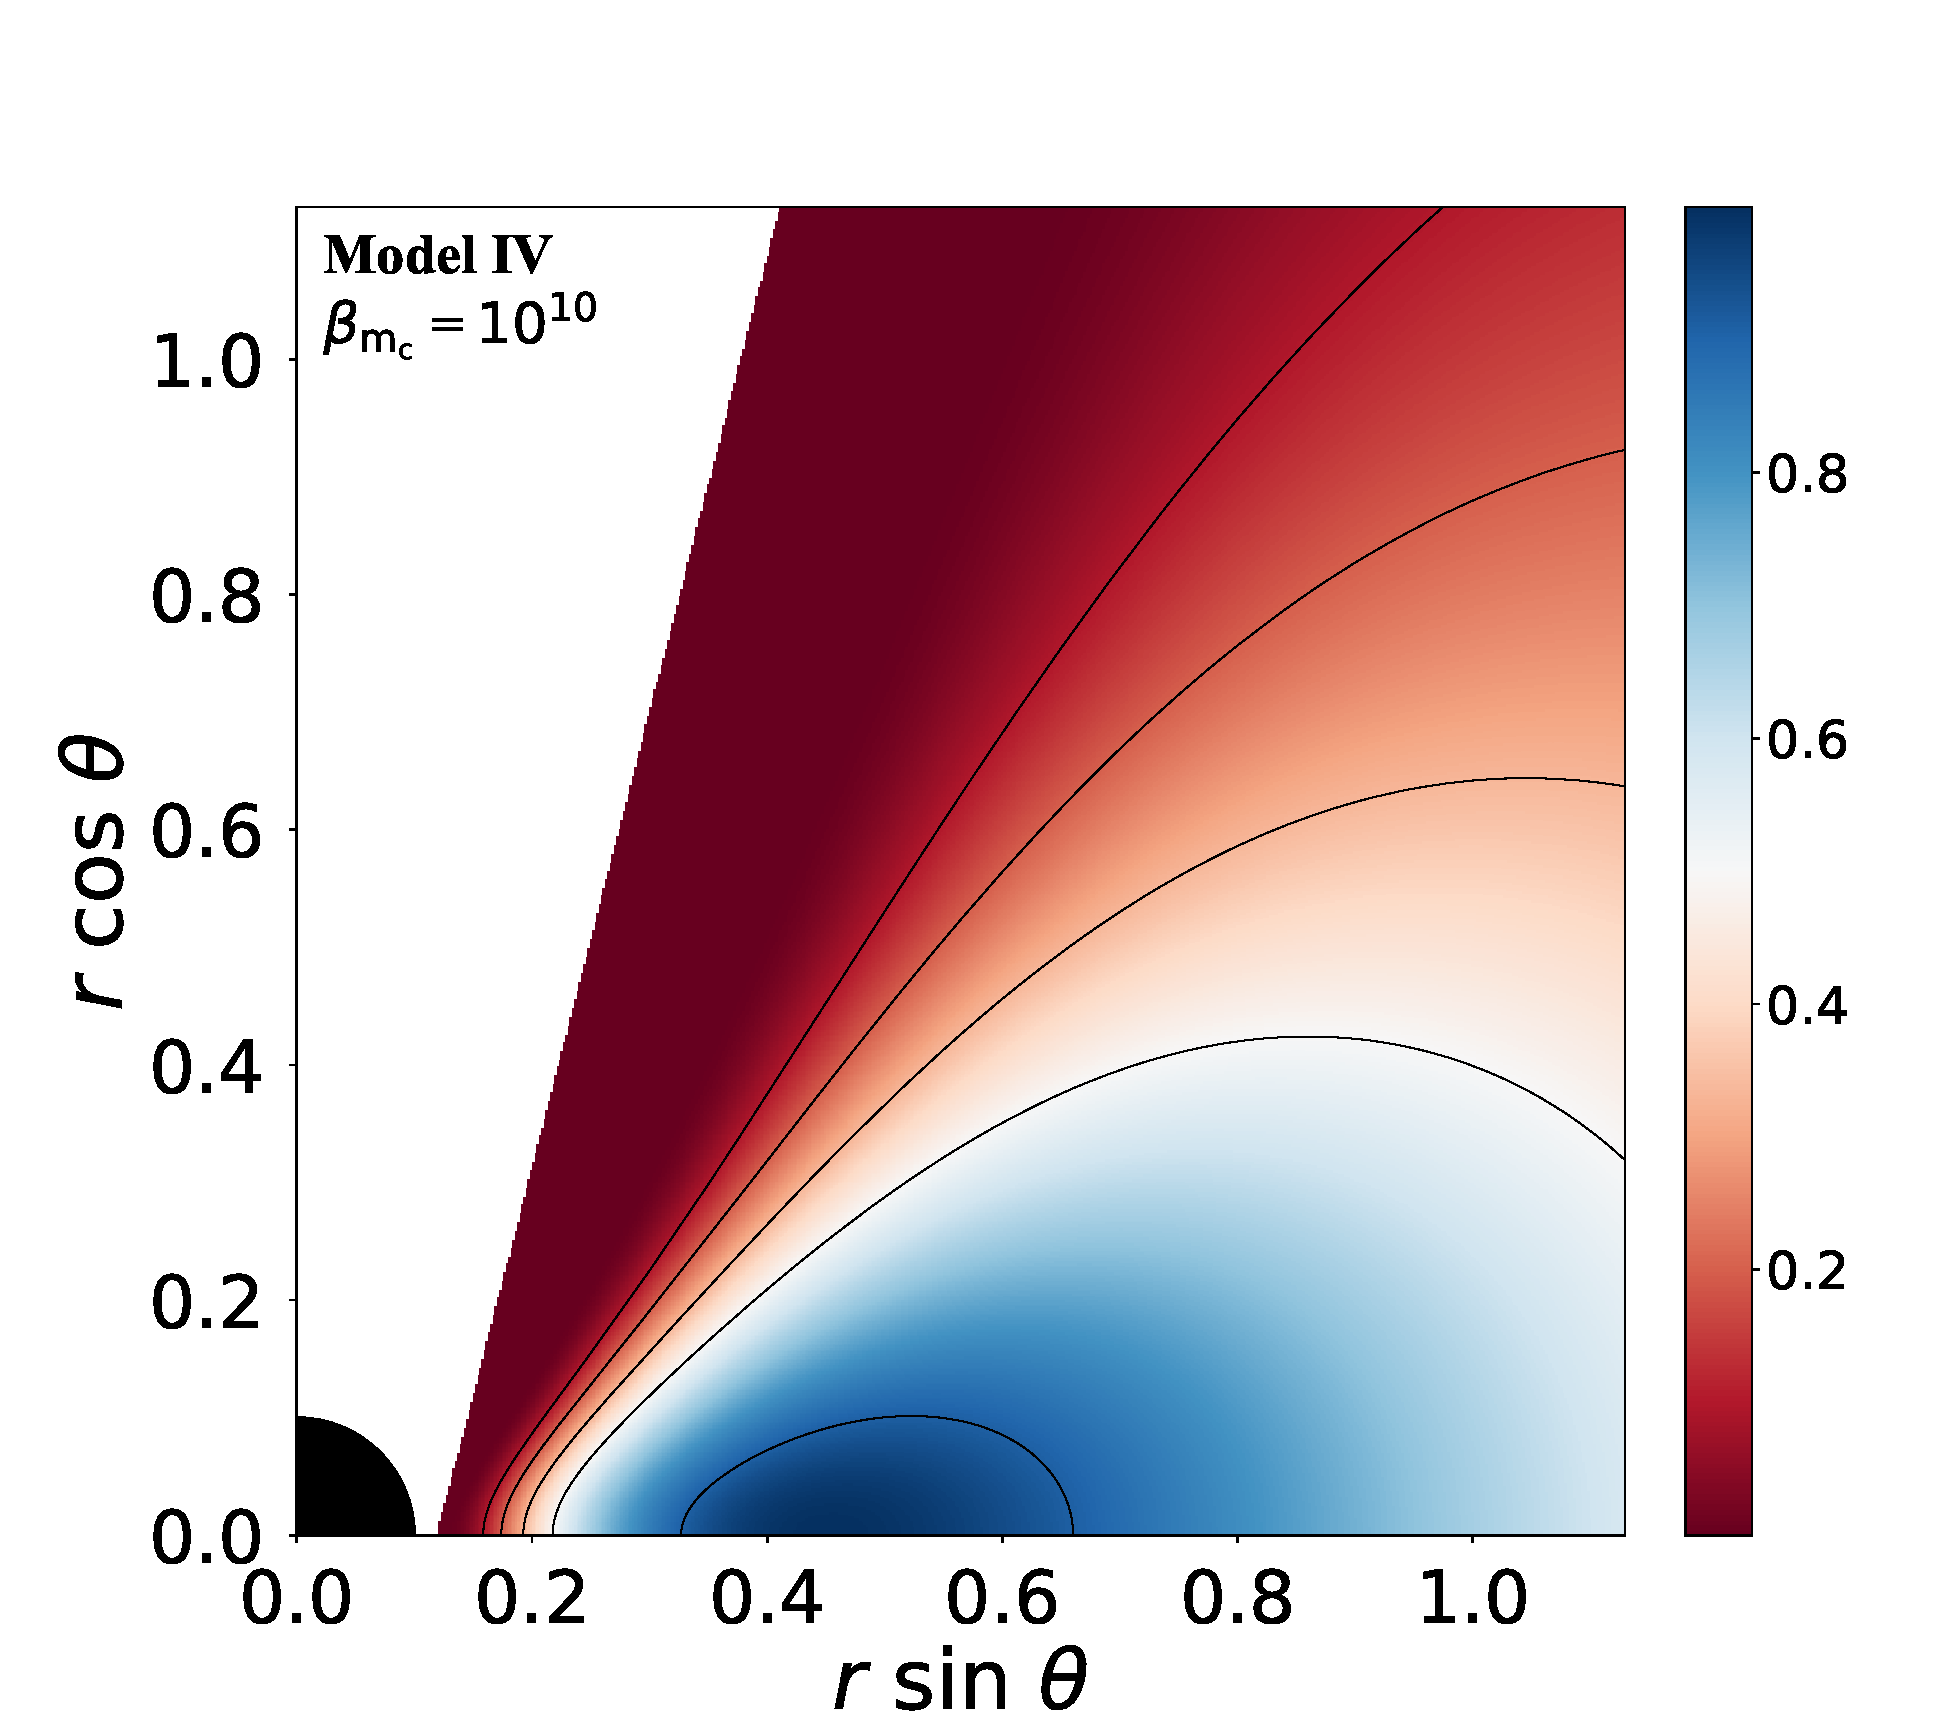
\includegraphics[scale=0.14]{figures/fig1_IV_10.pdf}
\hspace{-0.3cm}
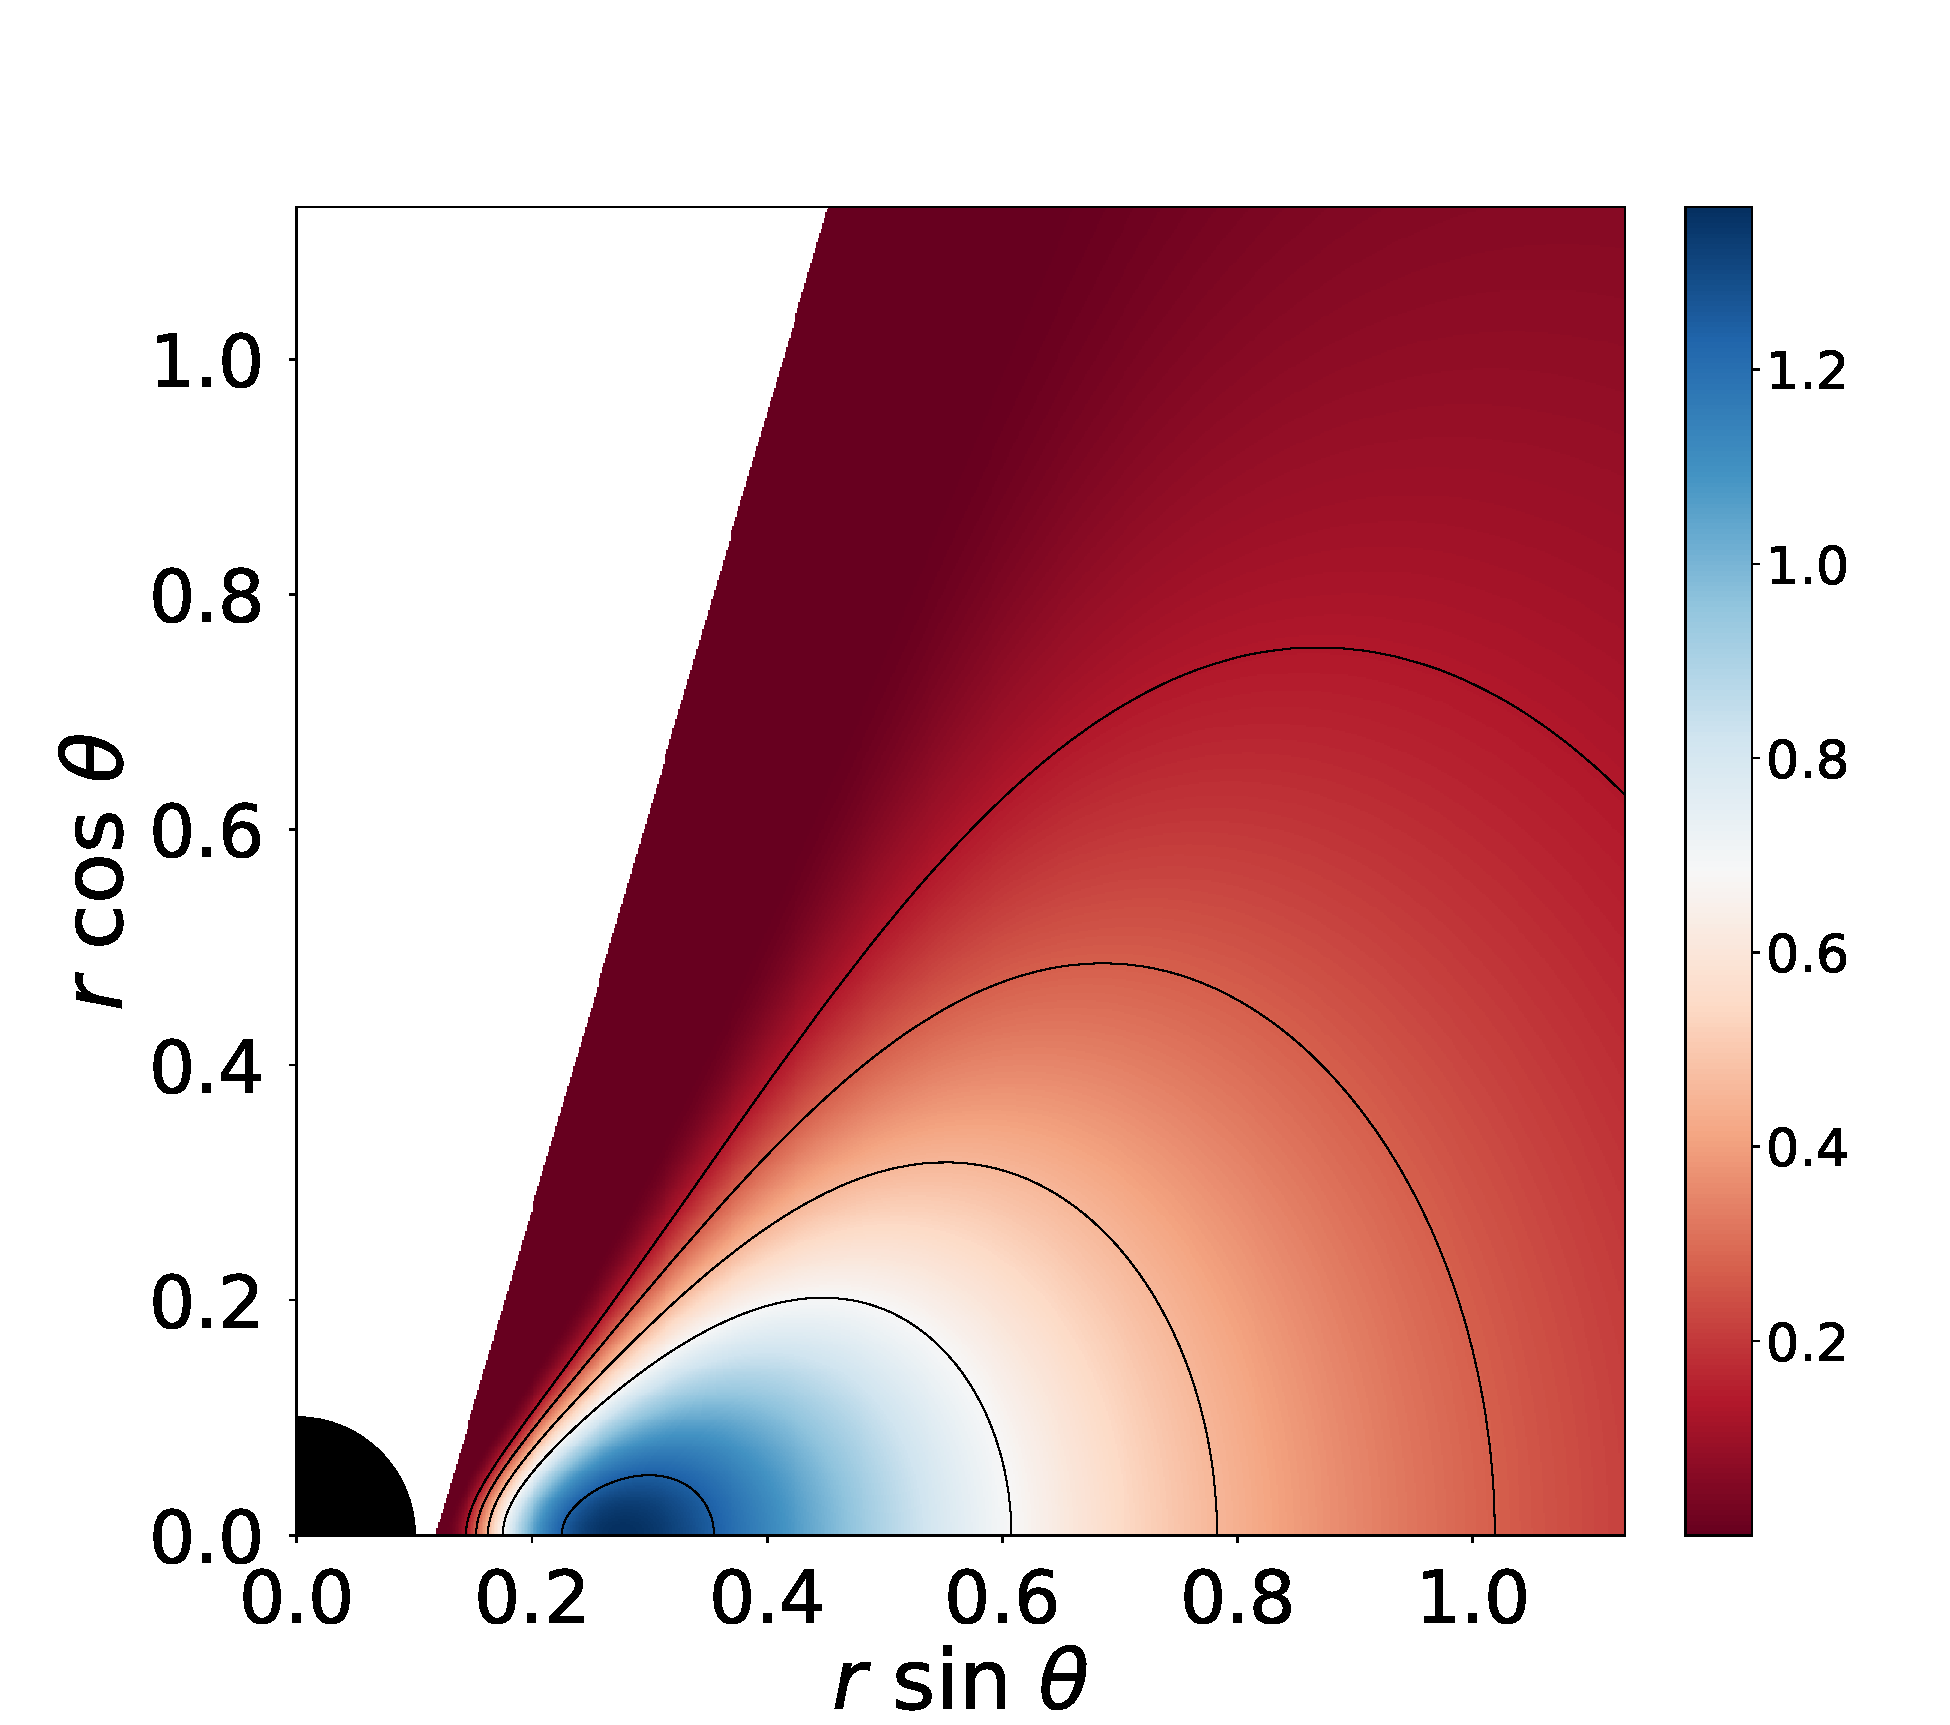
\includegraphics[scale=0.14]{figures/fig1_IV_1.pdf}
\hspace{-0.2cm}
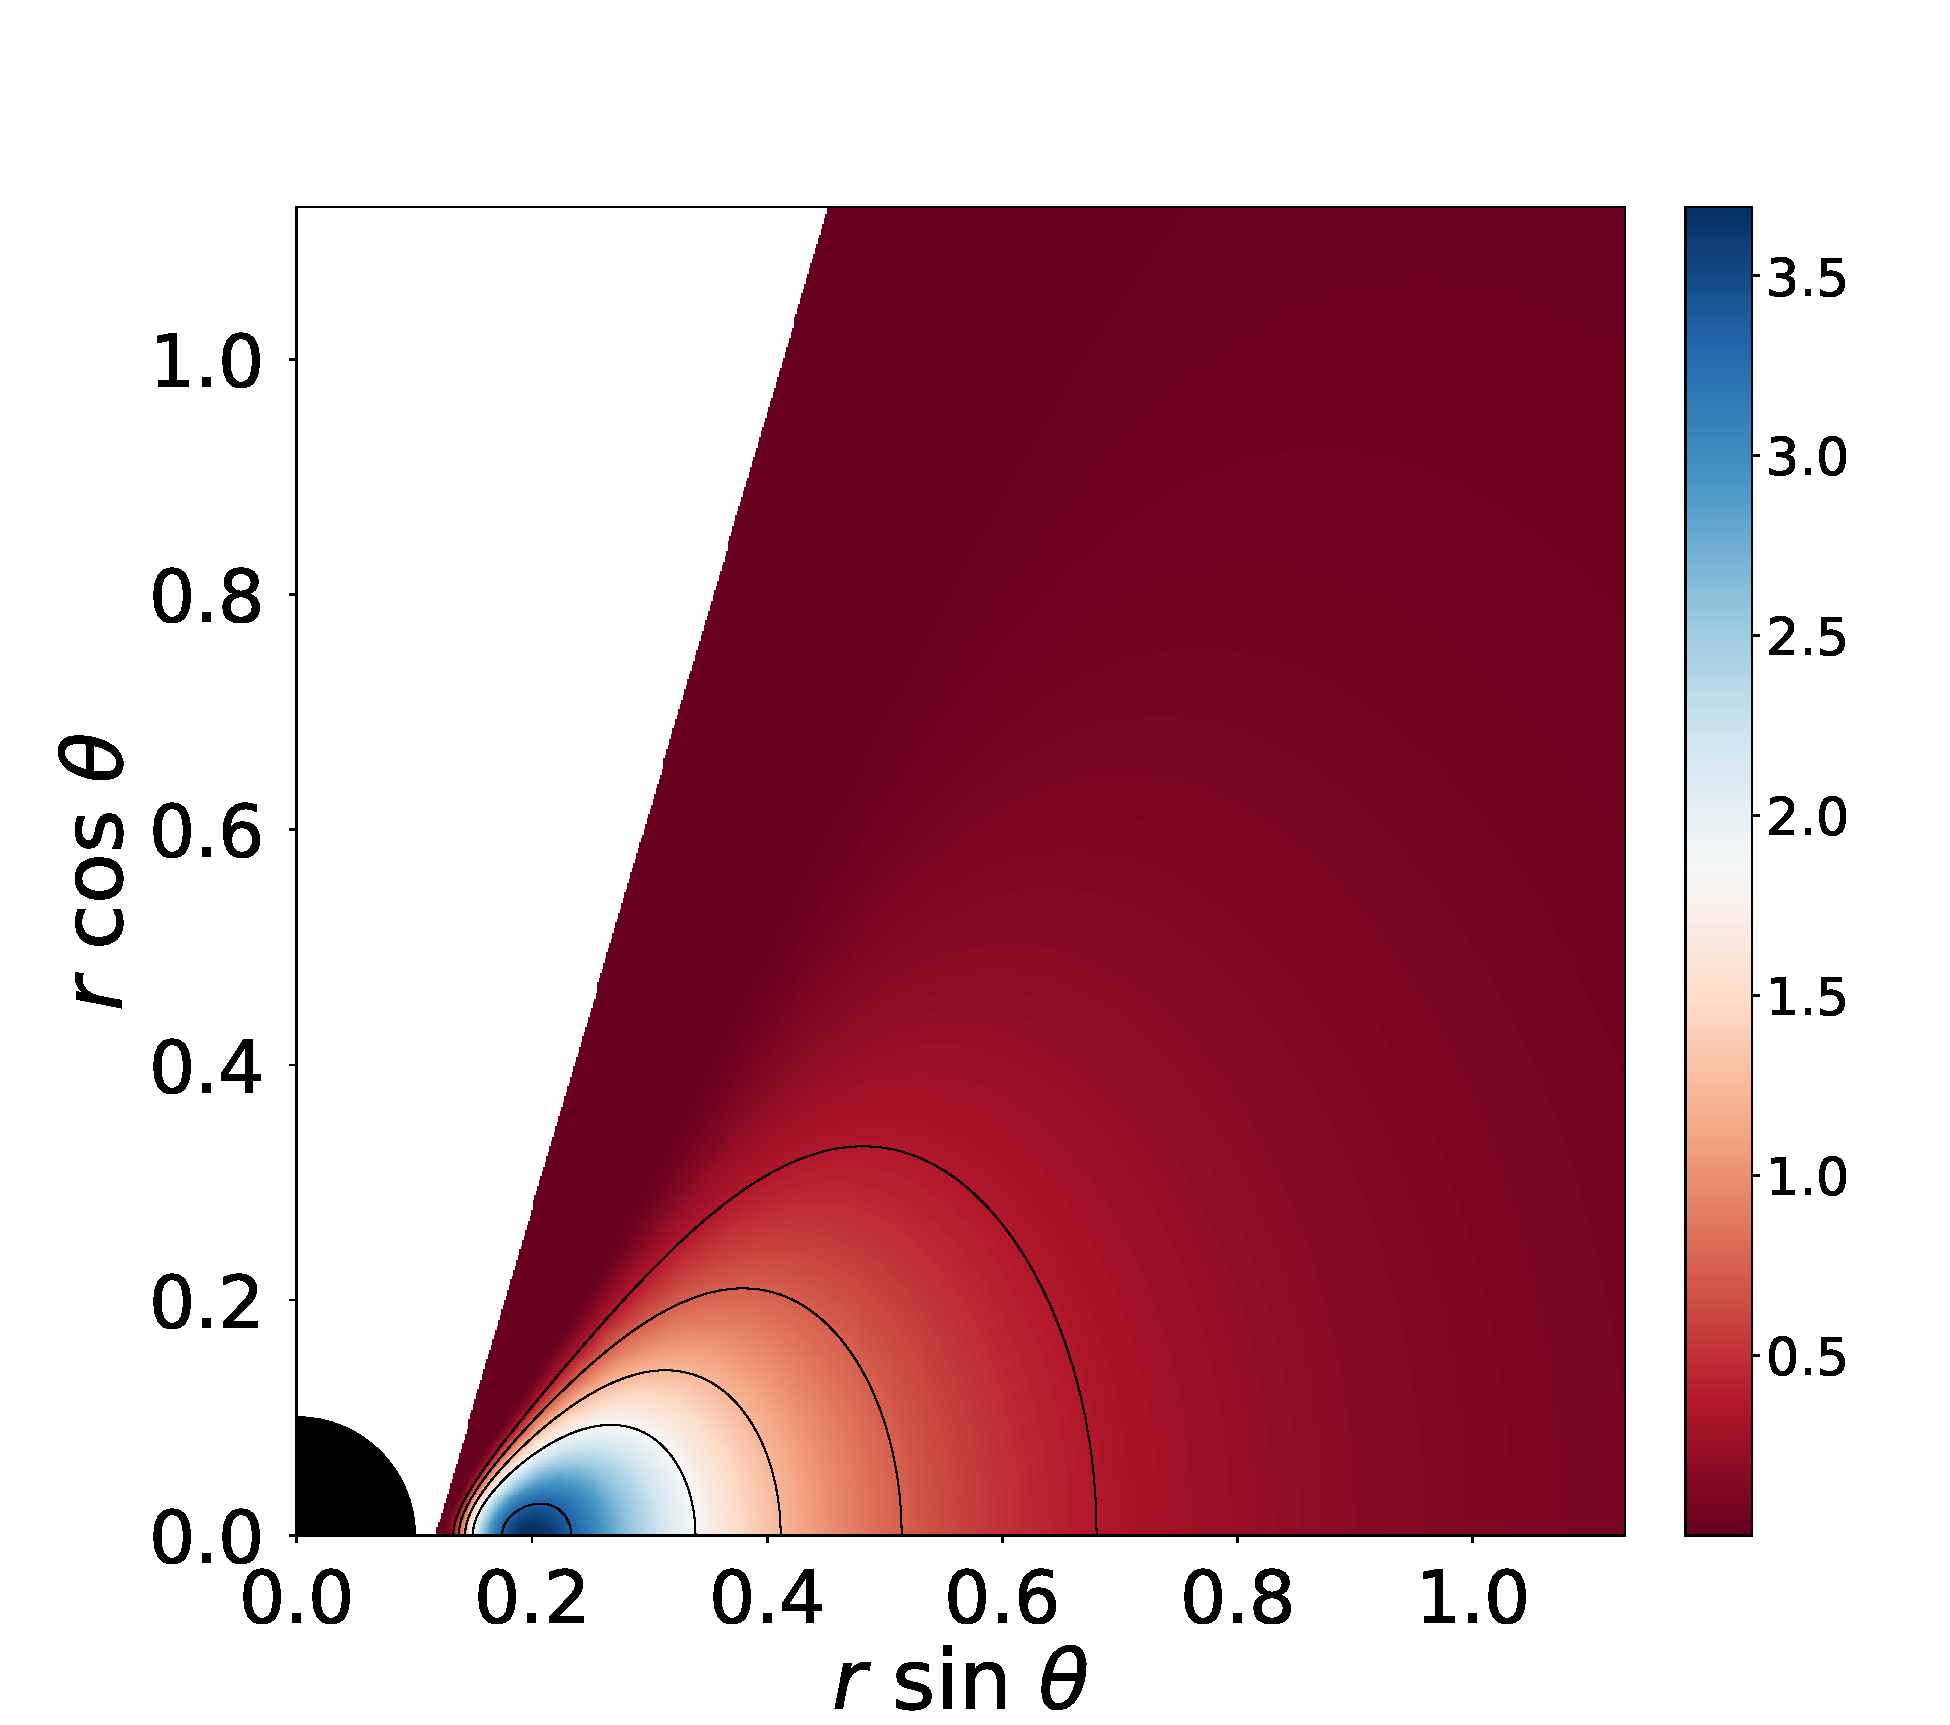
\includegraphics[scale=0.14]{figures/fig1_IV__10.pdf}
\hspace{-0.2cm}
\caption{Distribution of the rest-mass density. From top to bottom the rows correspond to the first four models of KBHsSH (I, II, III and IV). From left to right the columns correspond to different values of the magnetization parameter, namely non-magnetized ($\beta_{\mathrm{m}_{\mathrm{c}}} = 10^{10}$), mildly magnetized ($\beta_{\mathrm{m}_{\mathrm{c}}} = 1$) and strongly magnetized ($\beta_{\mathrm{m}_{\mathrm{c}}} = 10^{-10}$). Note that the range of the colour scale is not the same for all plots.}
\label{models_I}
\end{figure*}

\begin{figure*}
\centering
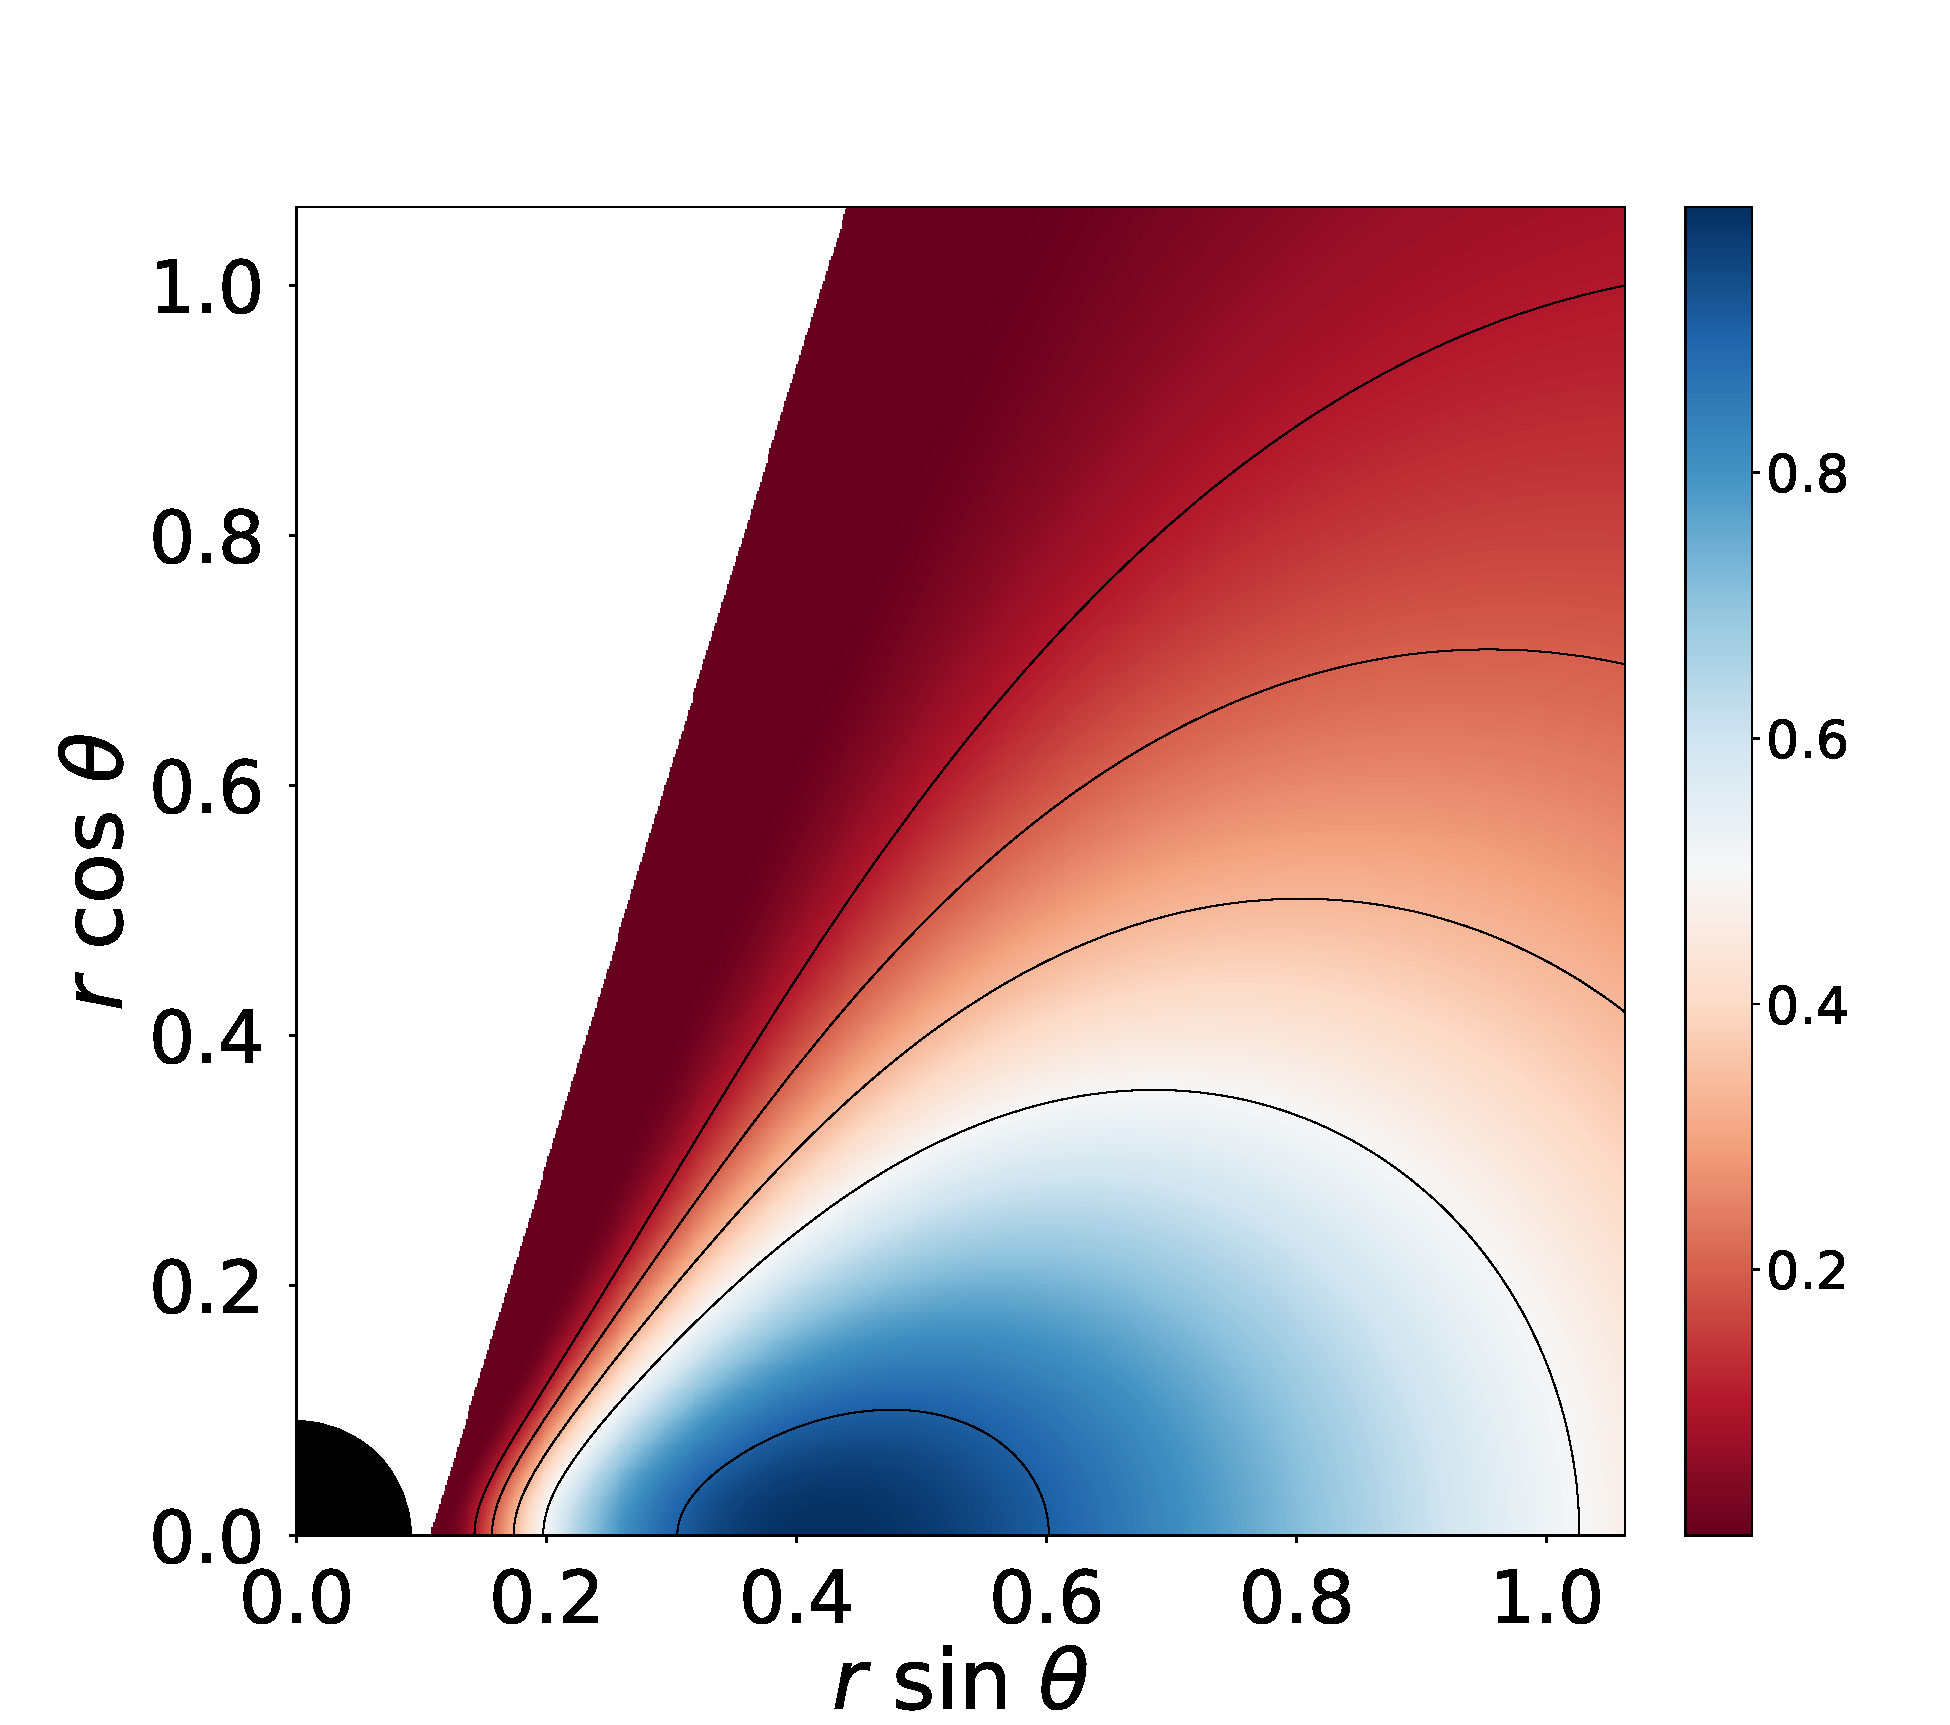
\includegraphics[scale=0.14]{figures/fig2_V_10.pdf}
\hspace{-0.3cm}
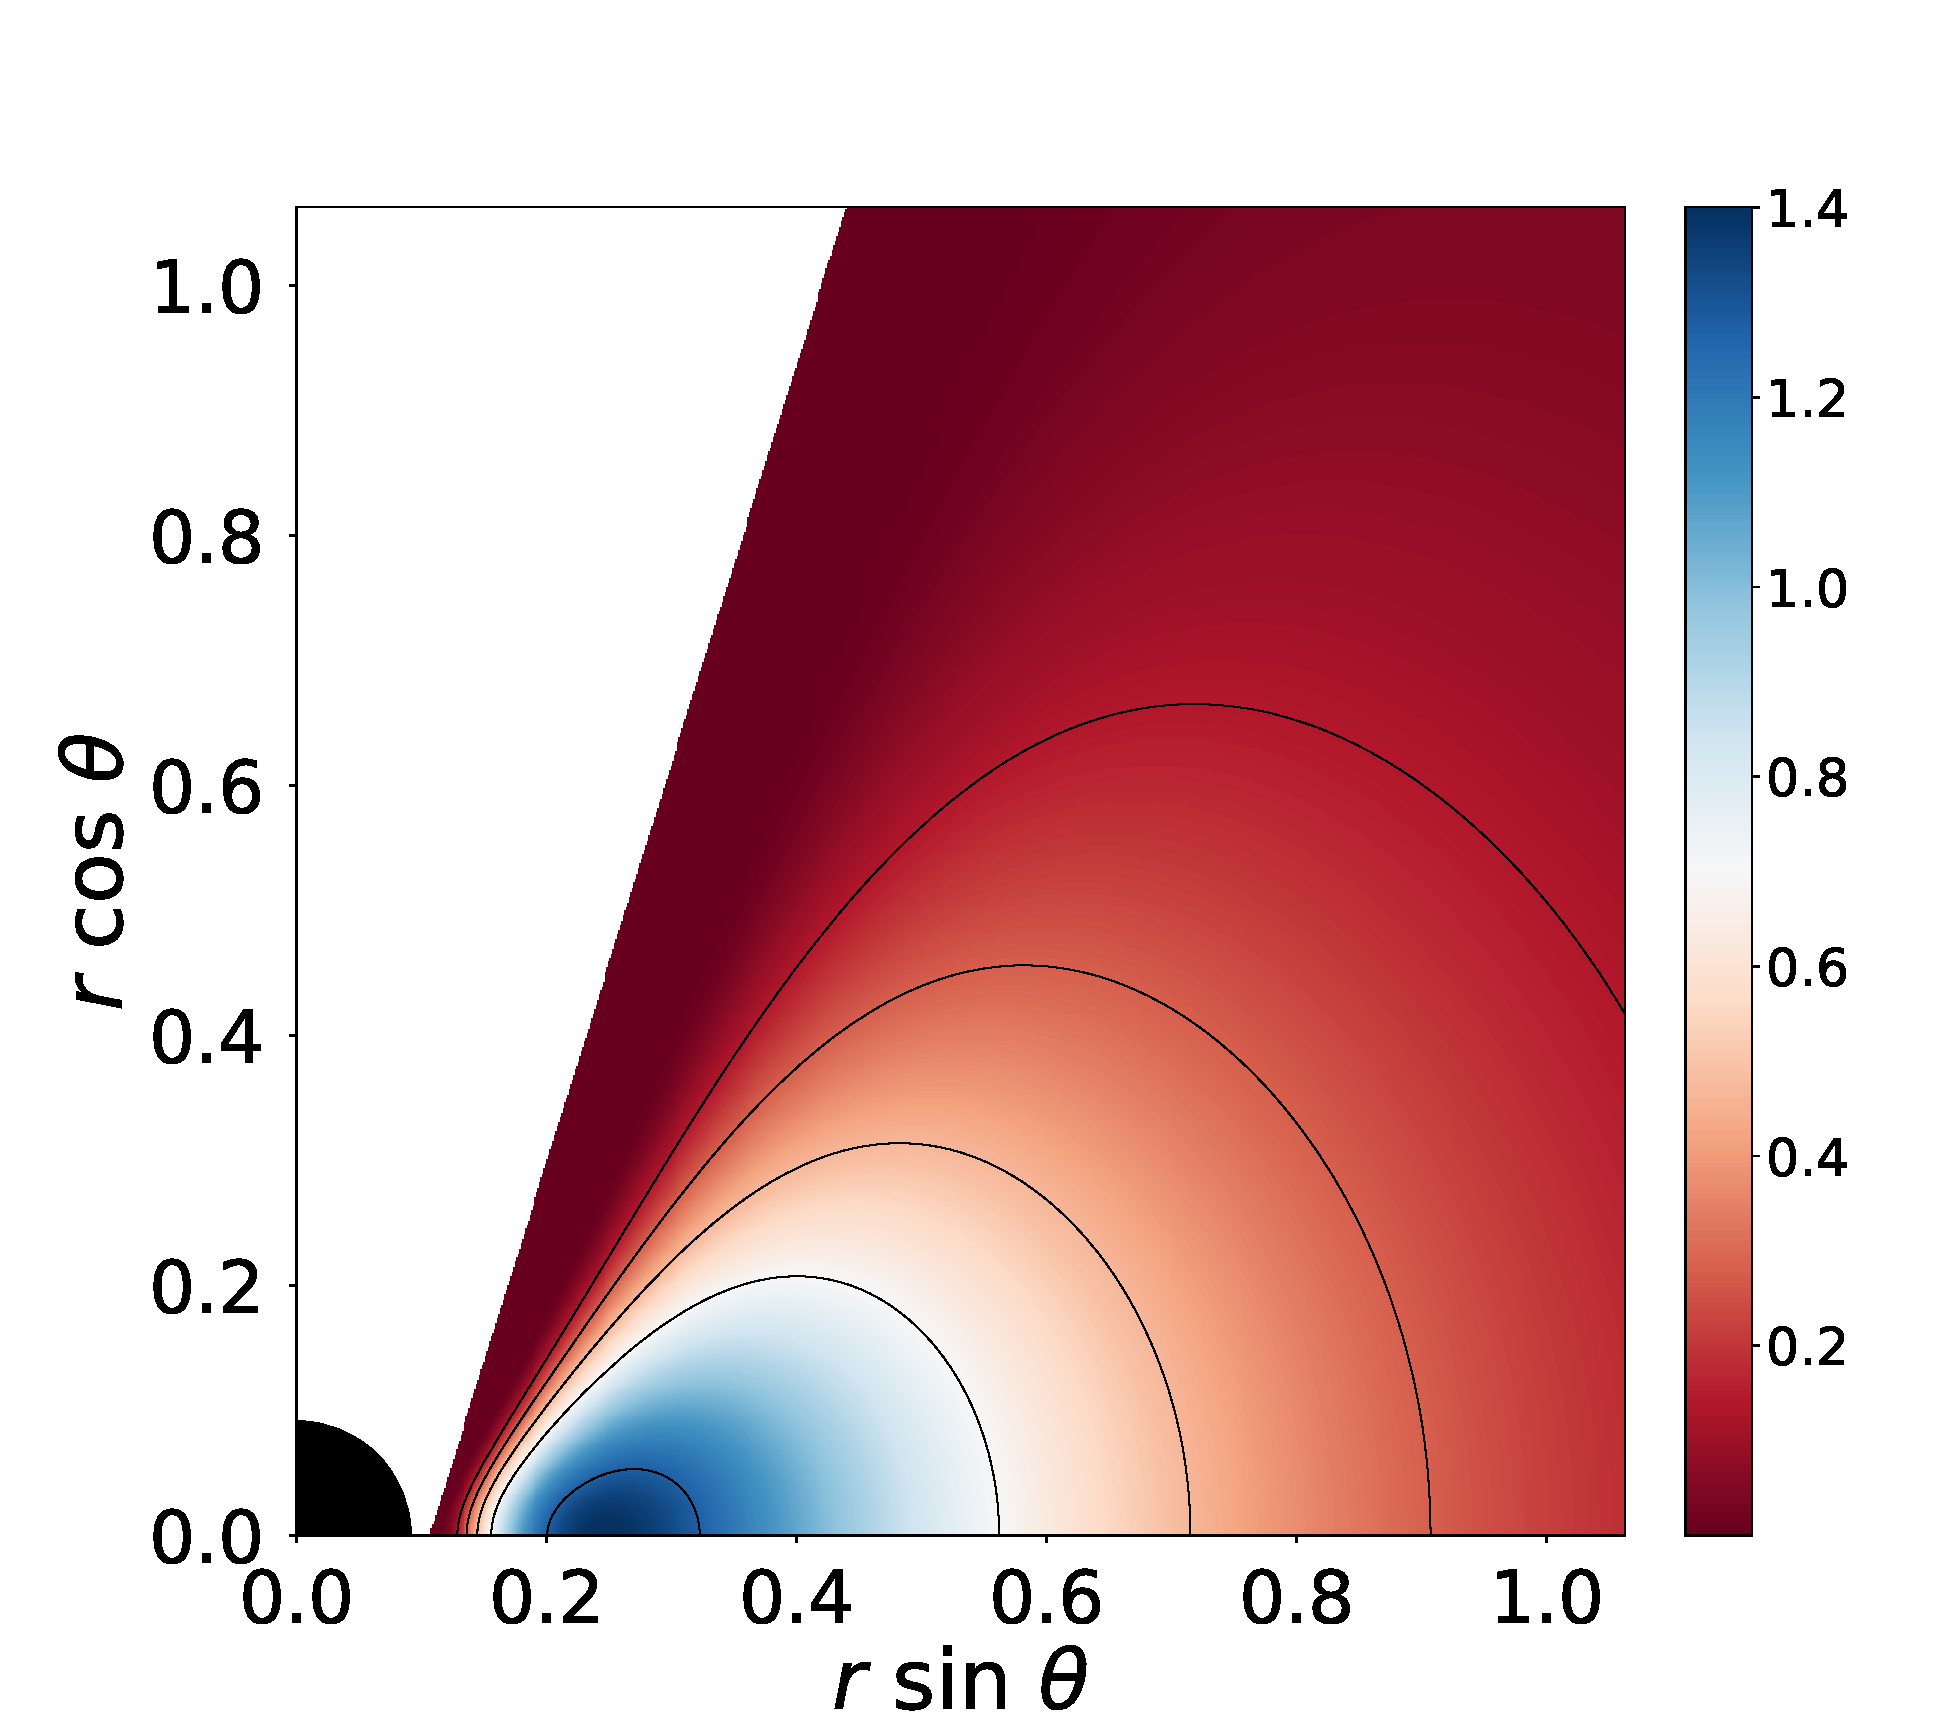
\includegraphics[scale=0.14]{figures/fig2_V_1.pdf}
\hspace{-0.2cm}
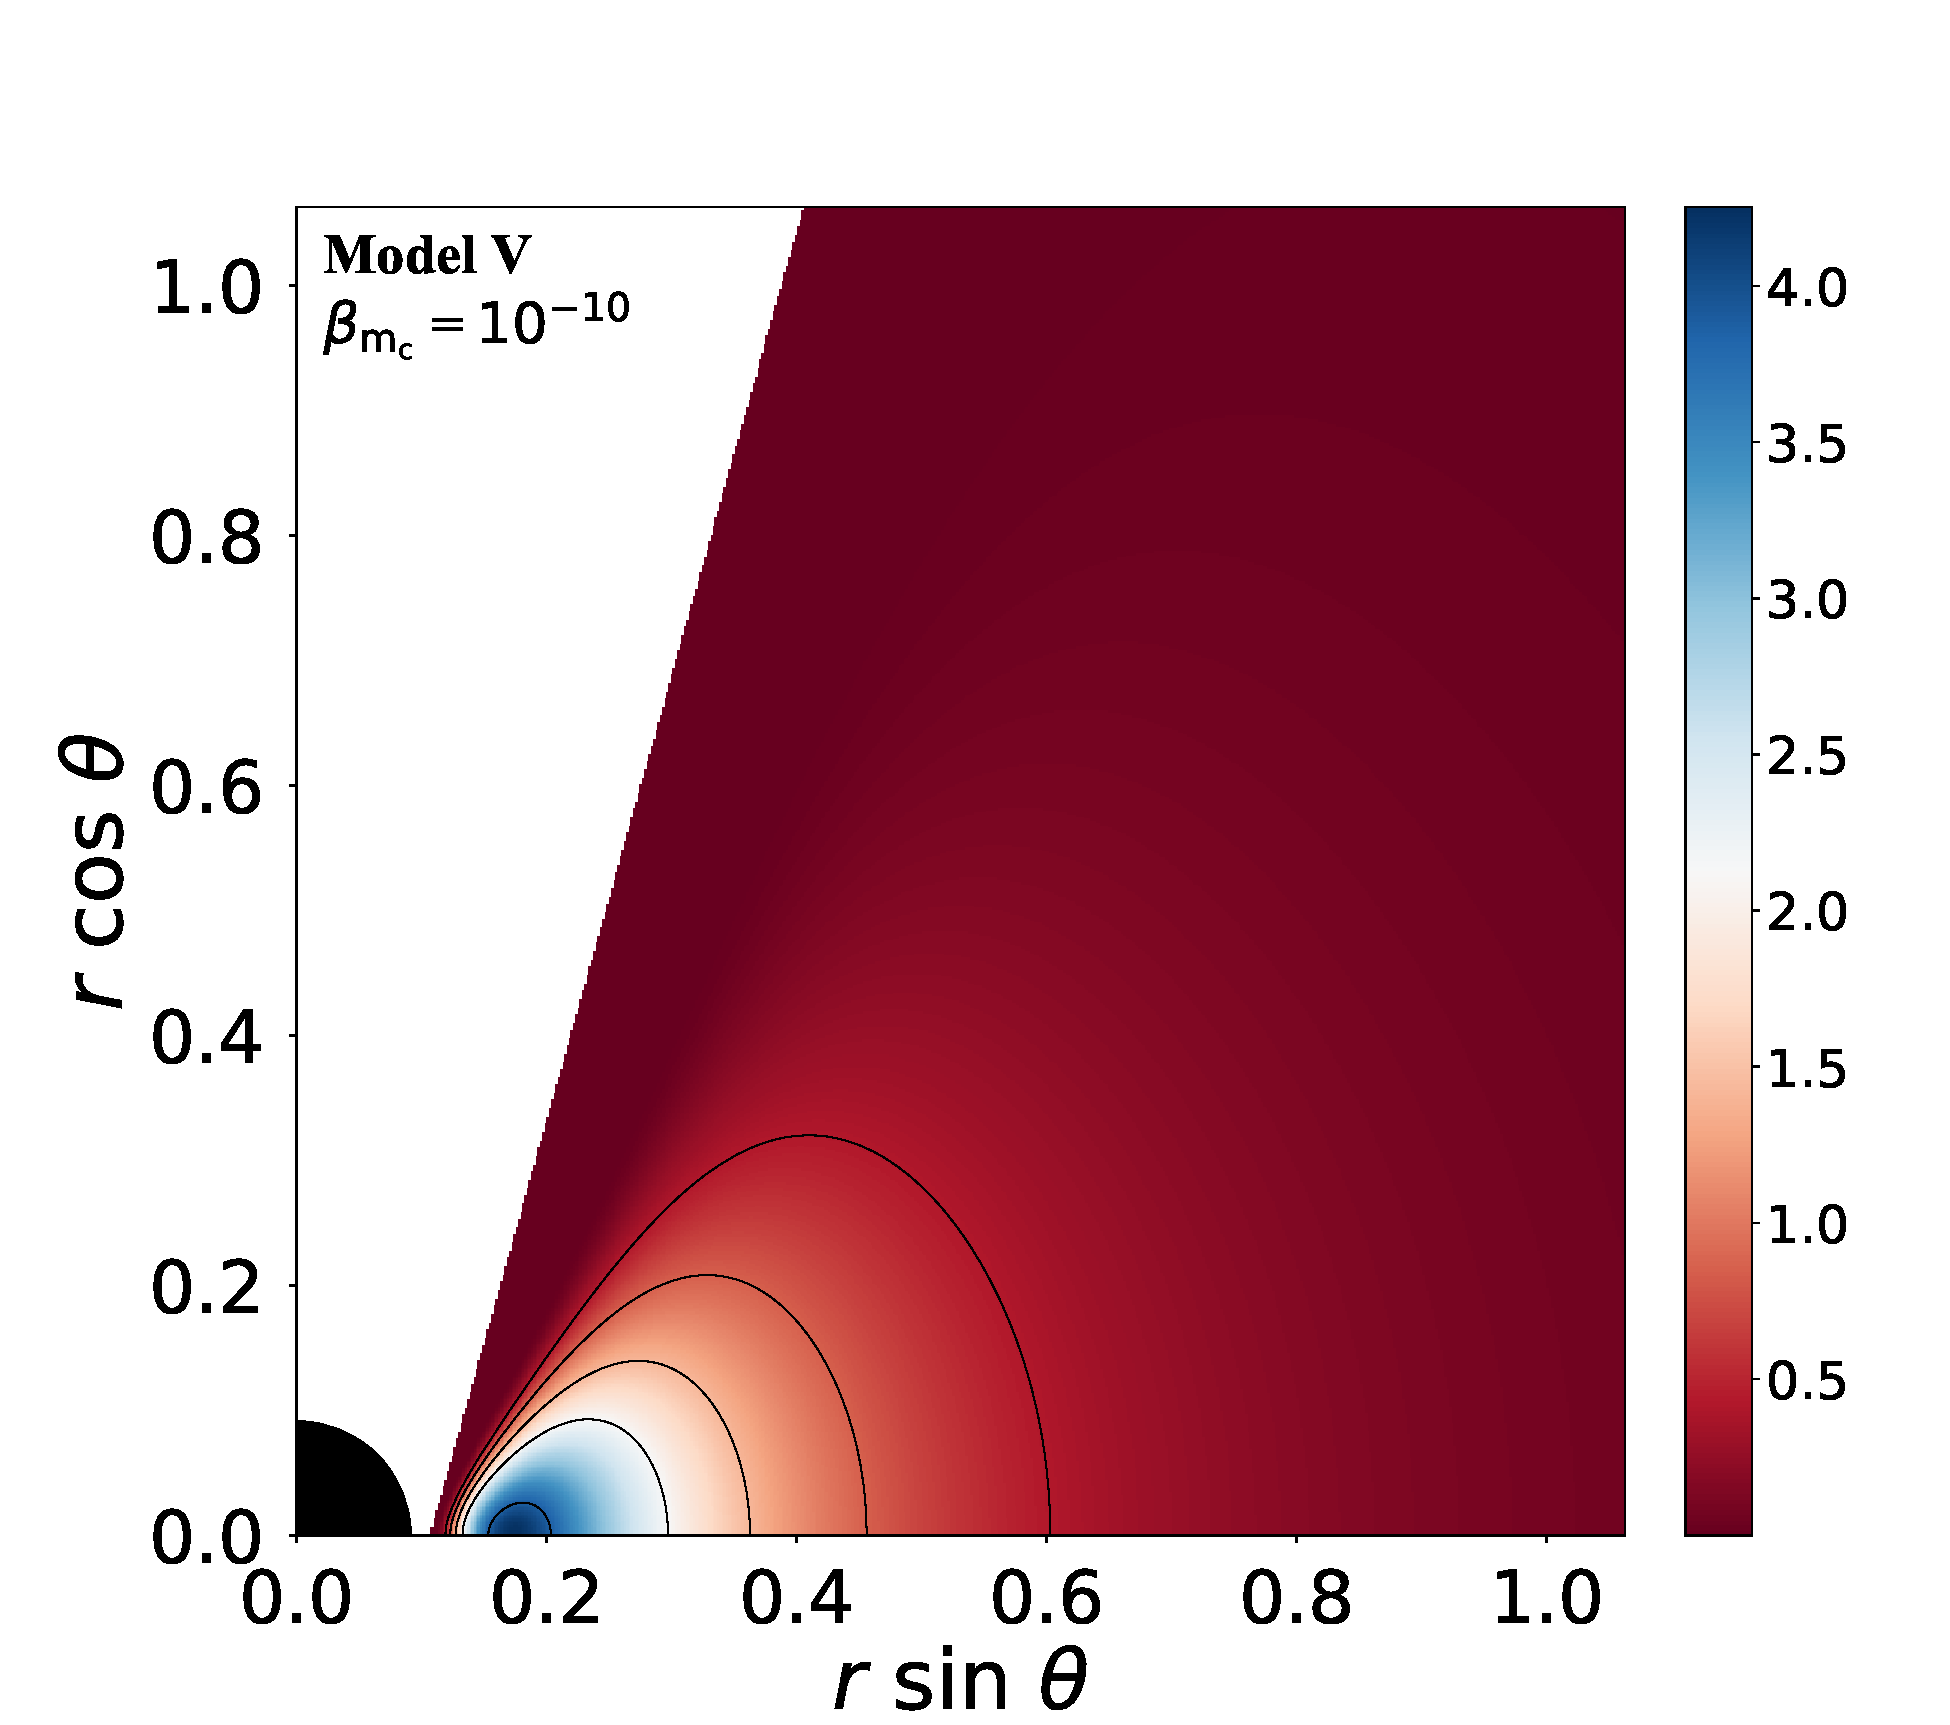
\includegraphics[scale=0.14]{figures/fig2_V__10.pdf}
\\
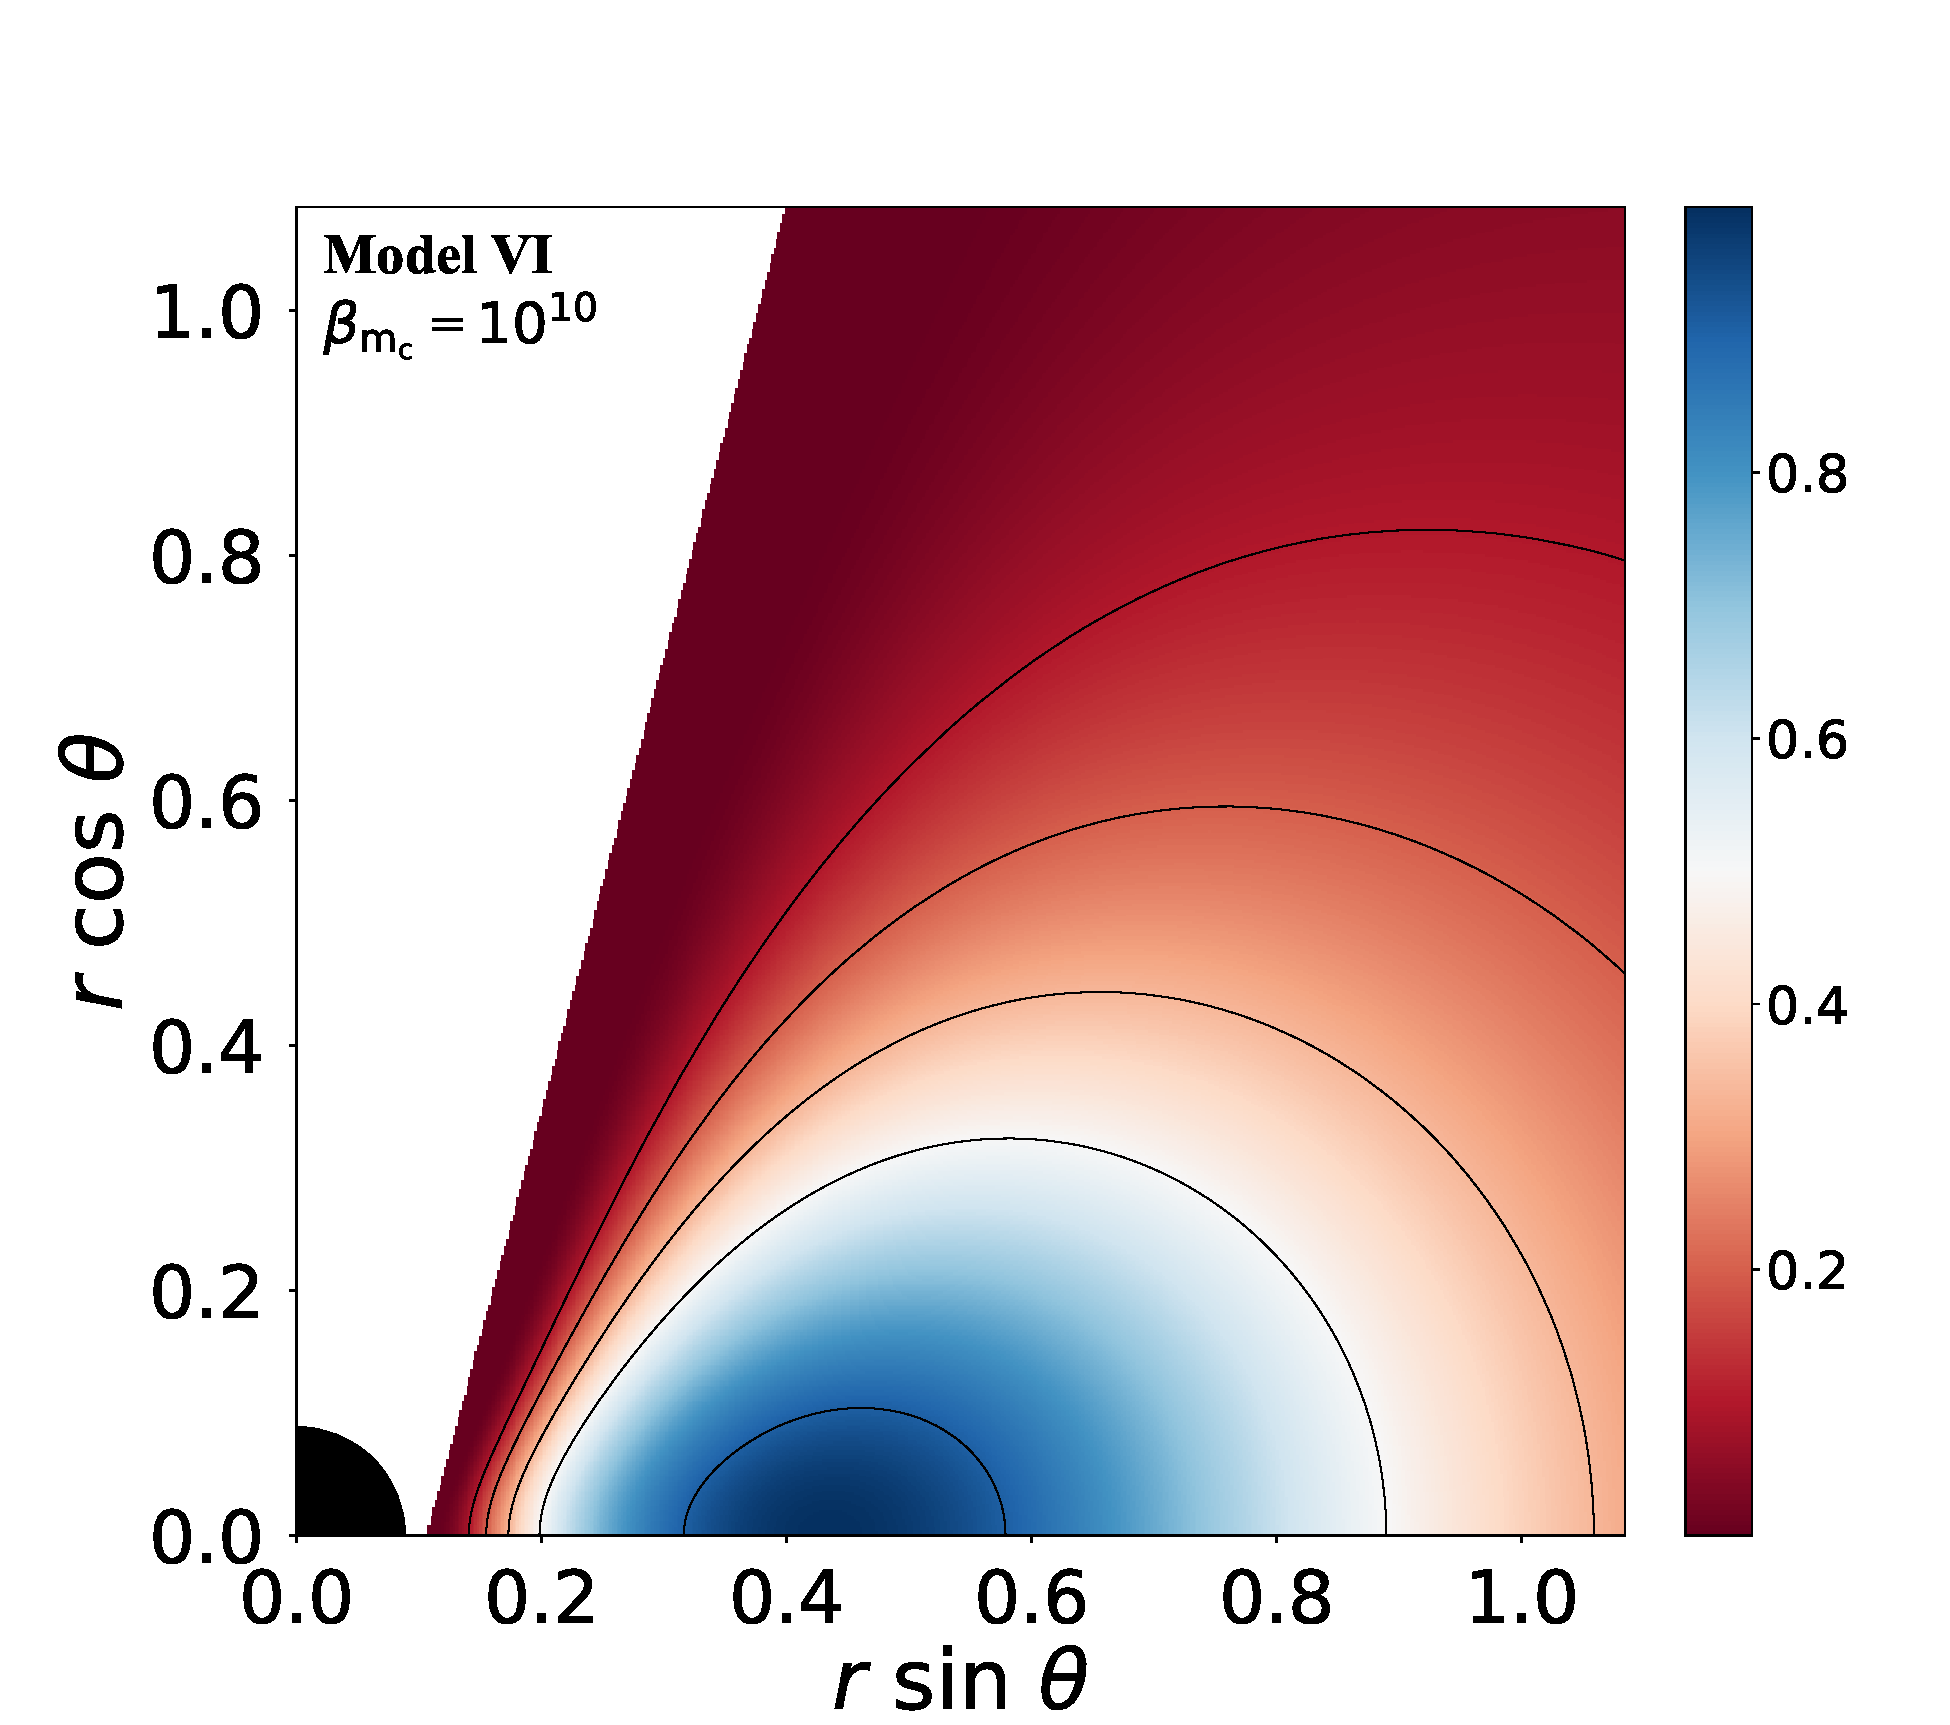
\includegraphics[scale=0.14]{figures/fig2_VI_10.pdf}
\hspace{-0.3cm}
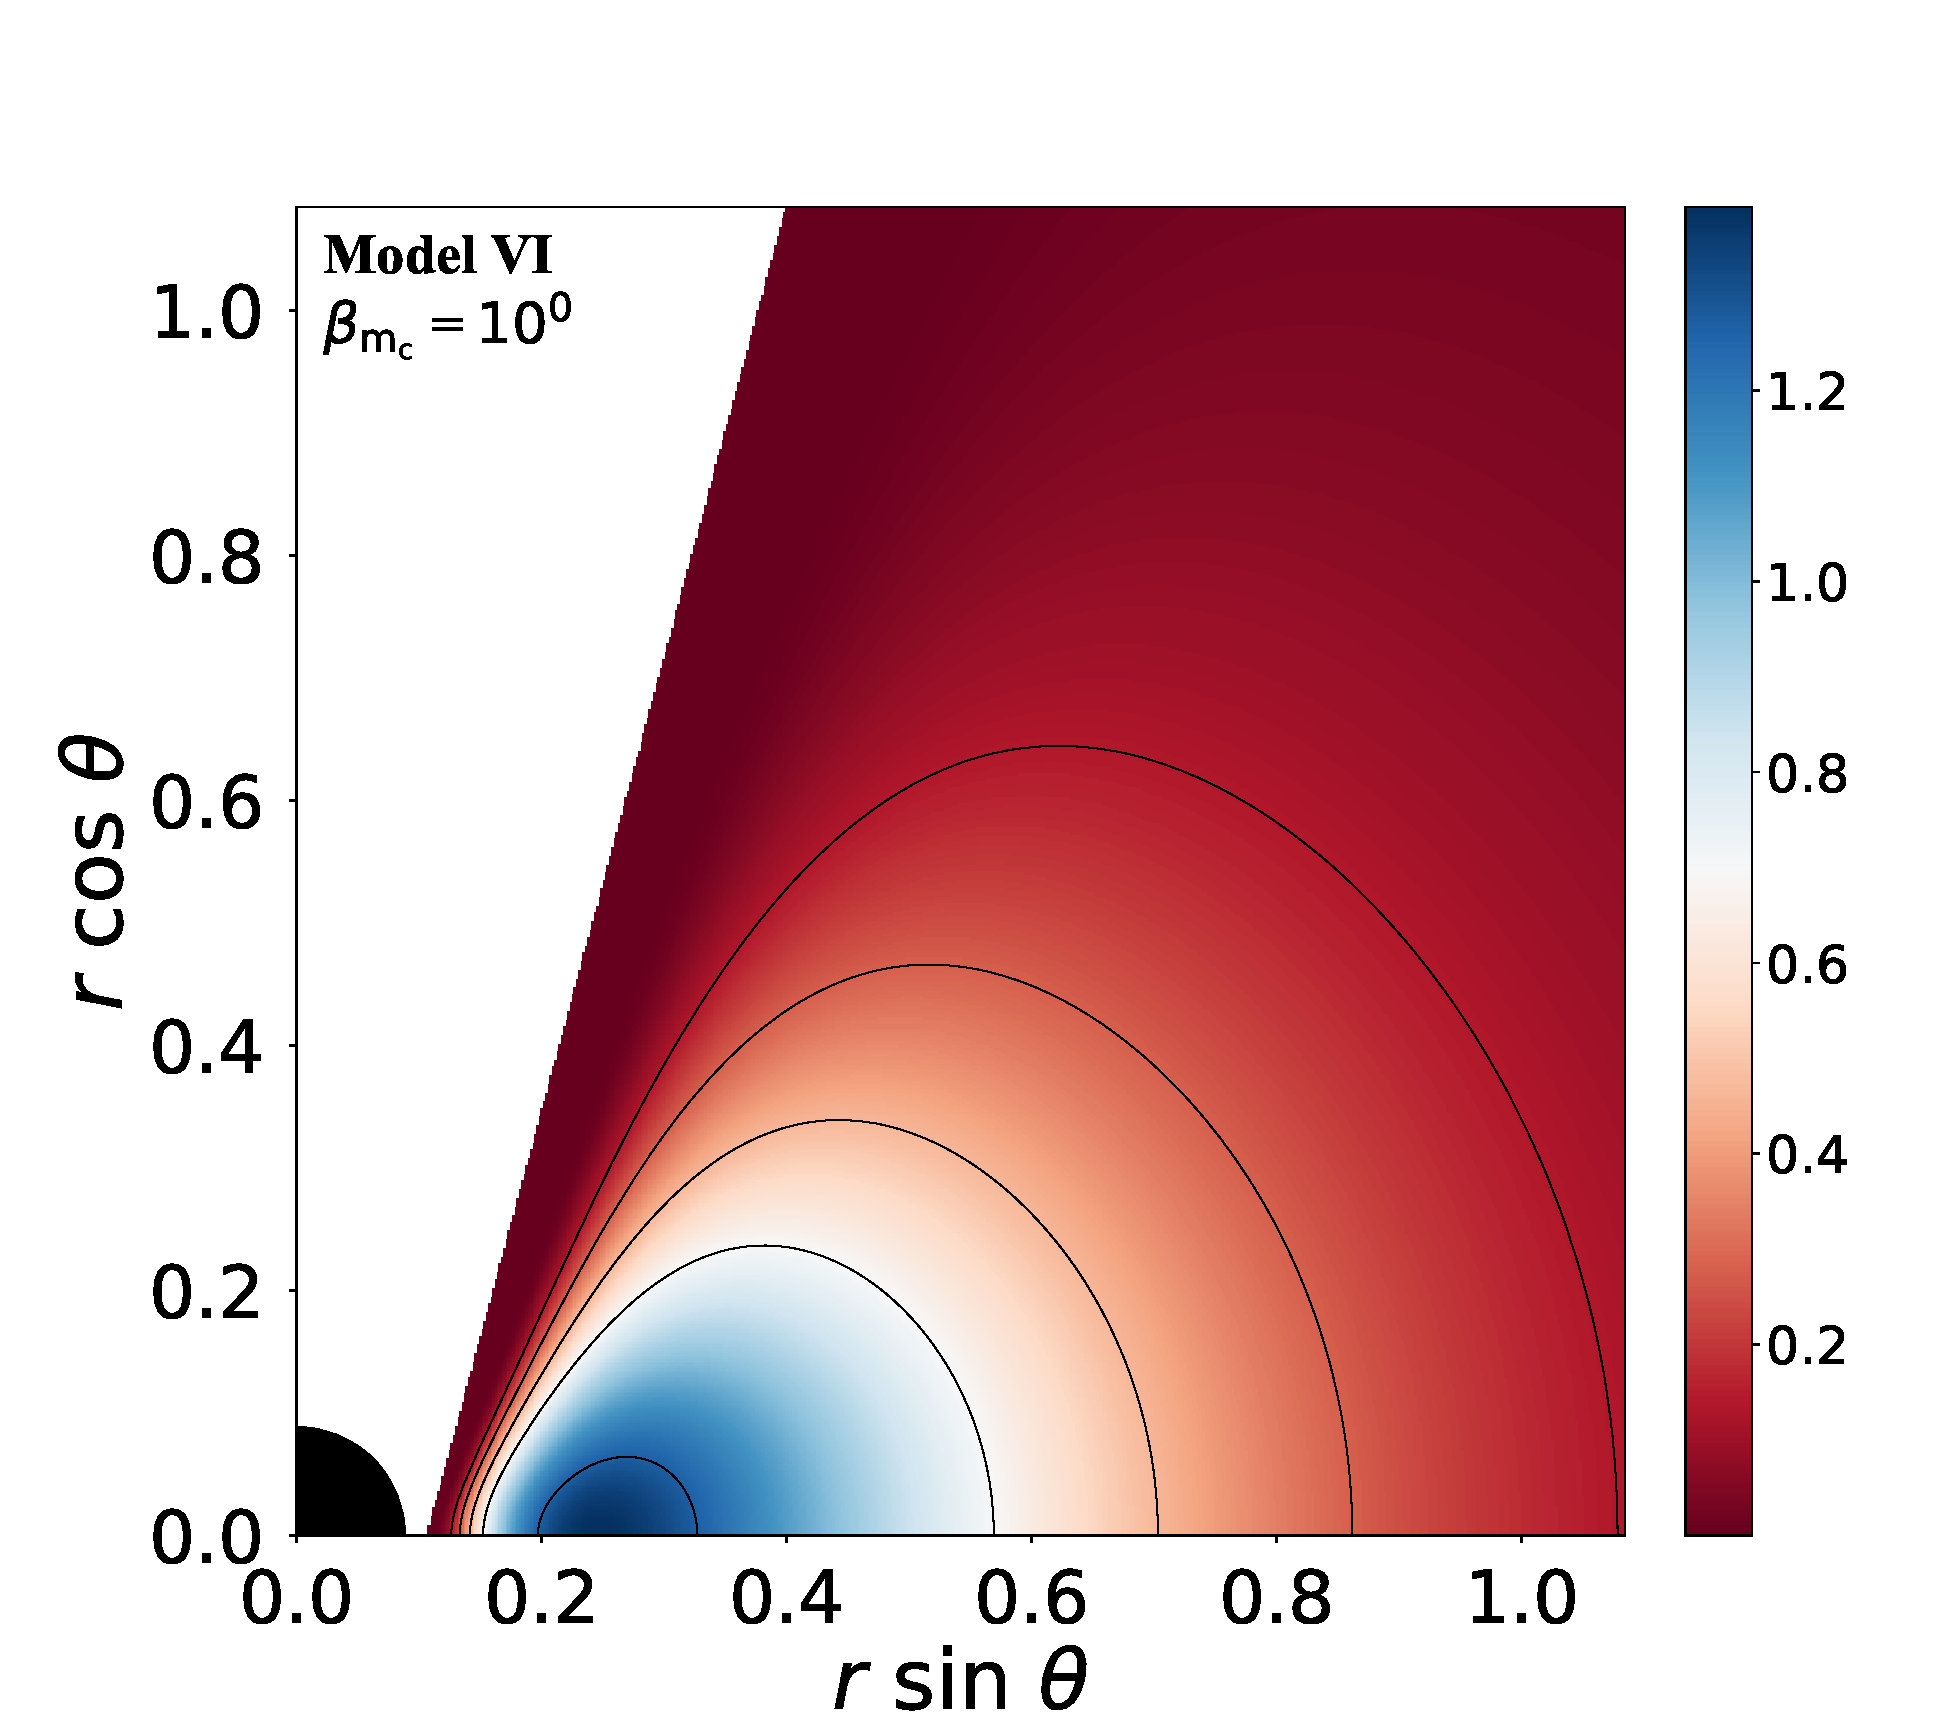
\includegraphics[scale=0.14]{figures/fig2_VI_1.pdf}
\hspace{-0.2cm}
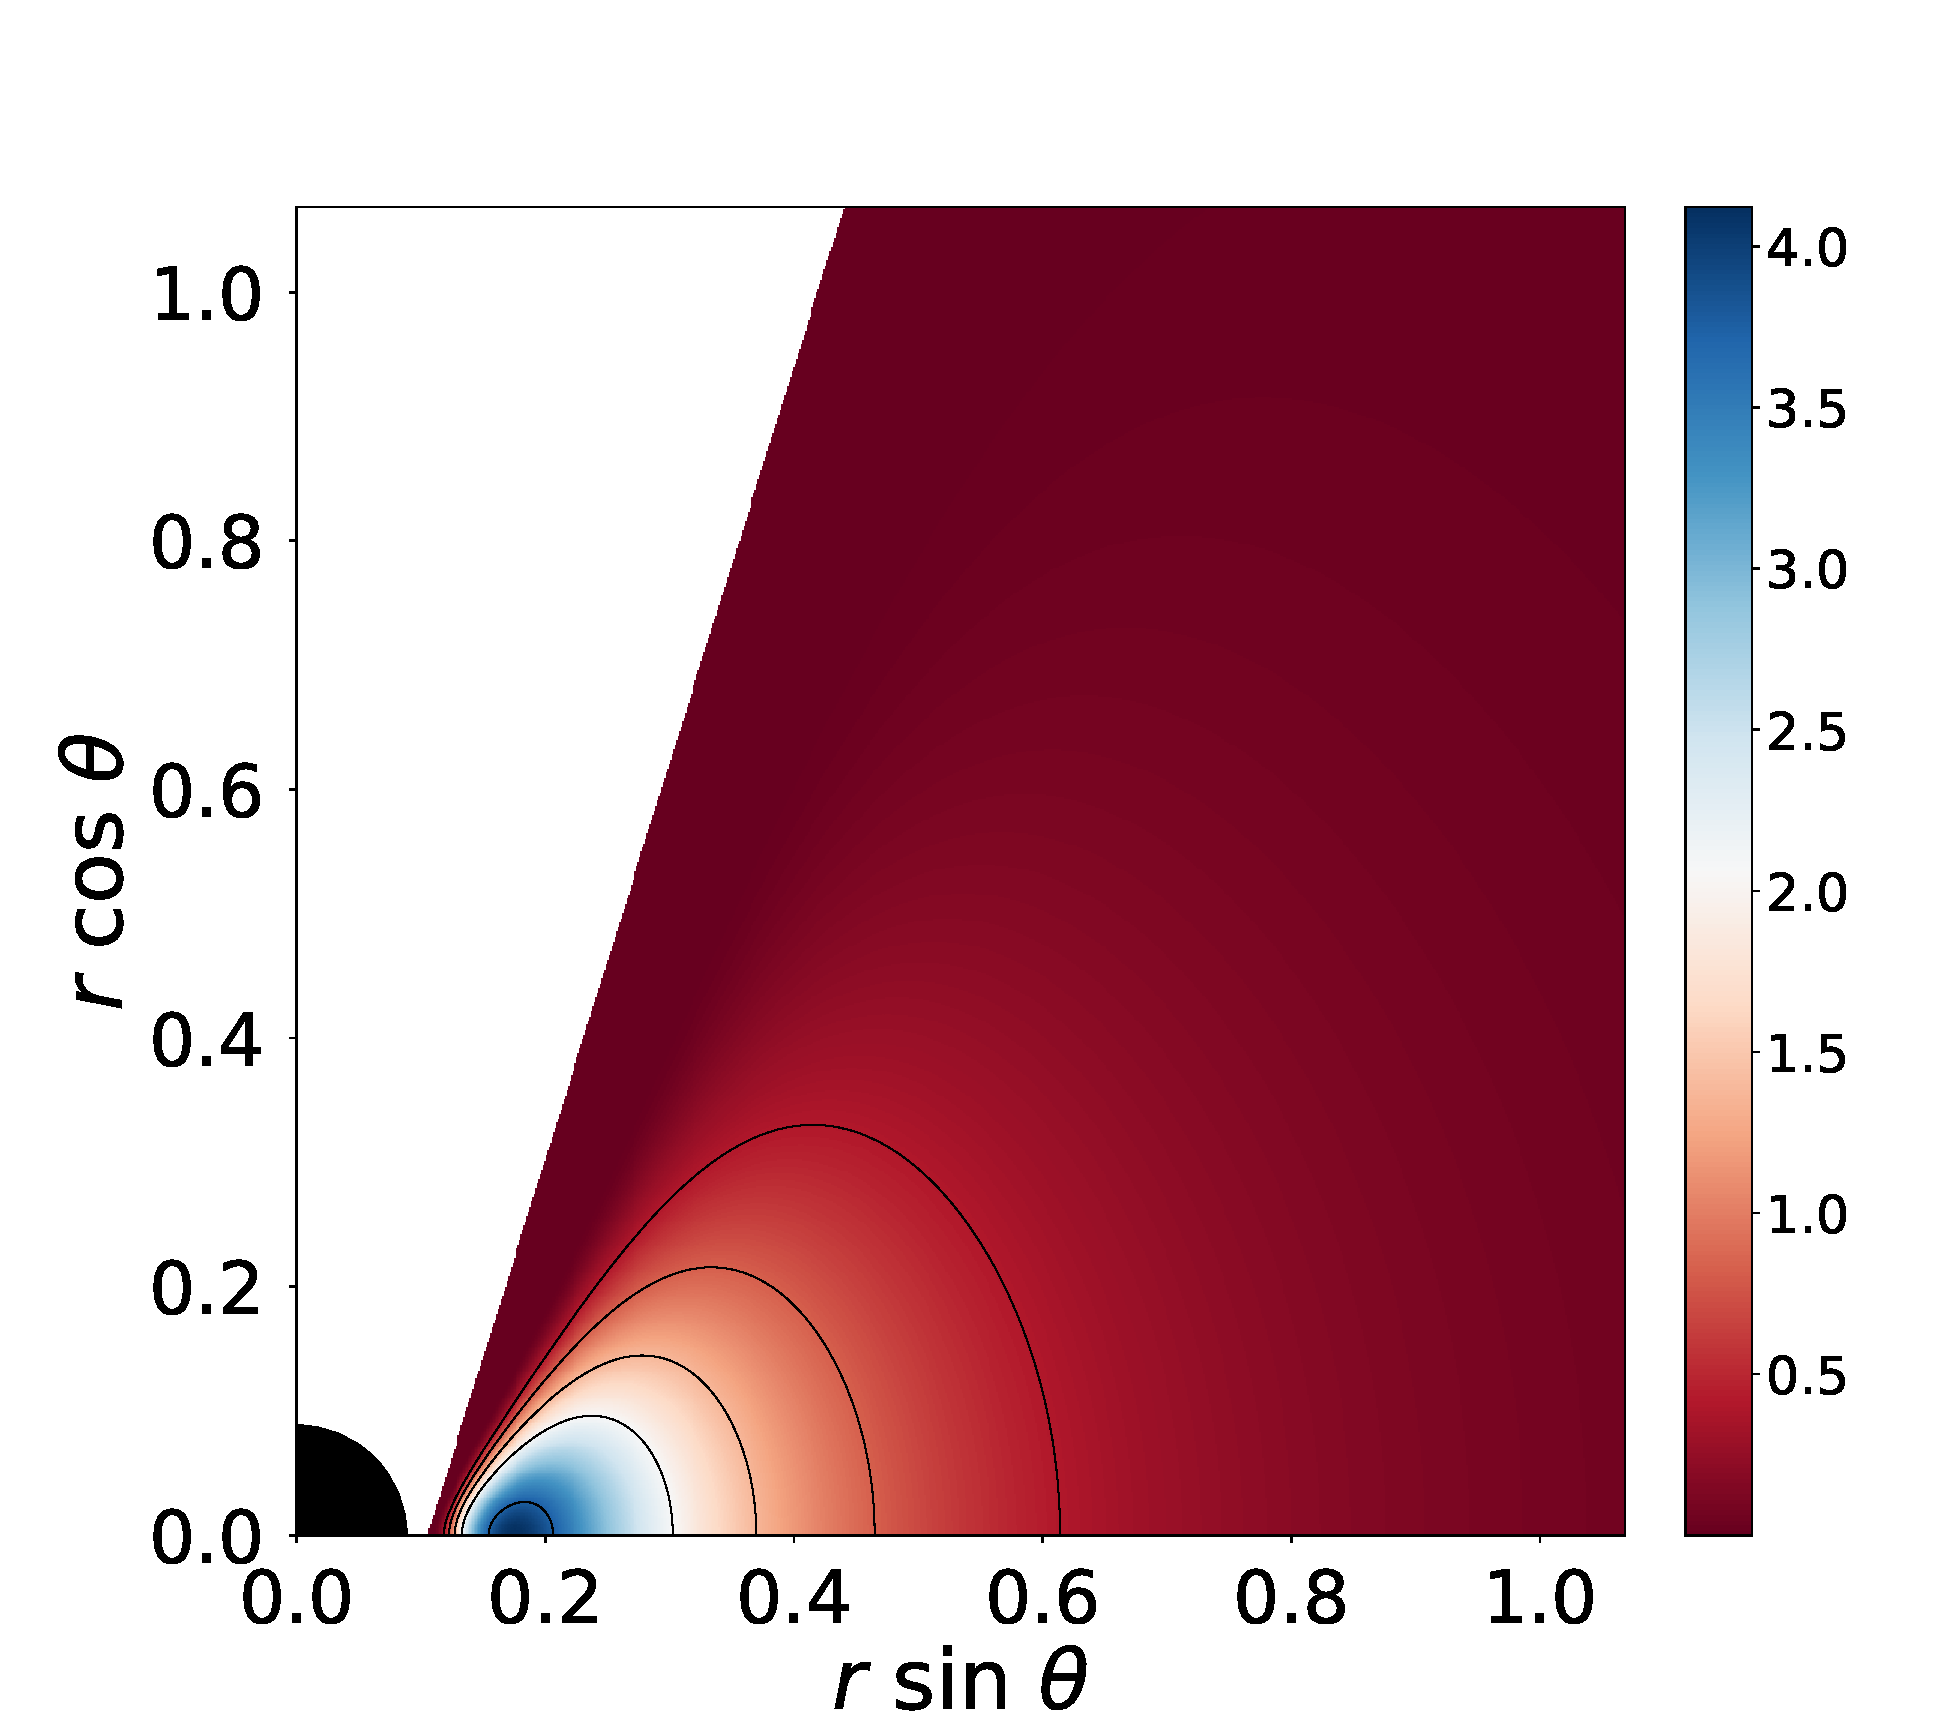
\includegraphics[scale=0.14]{figures/fig2_VI__10.pdf}
\\
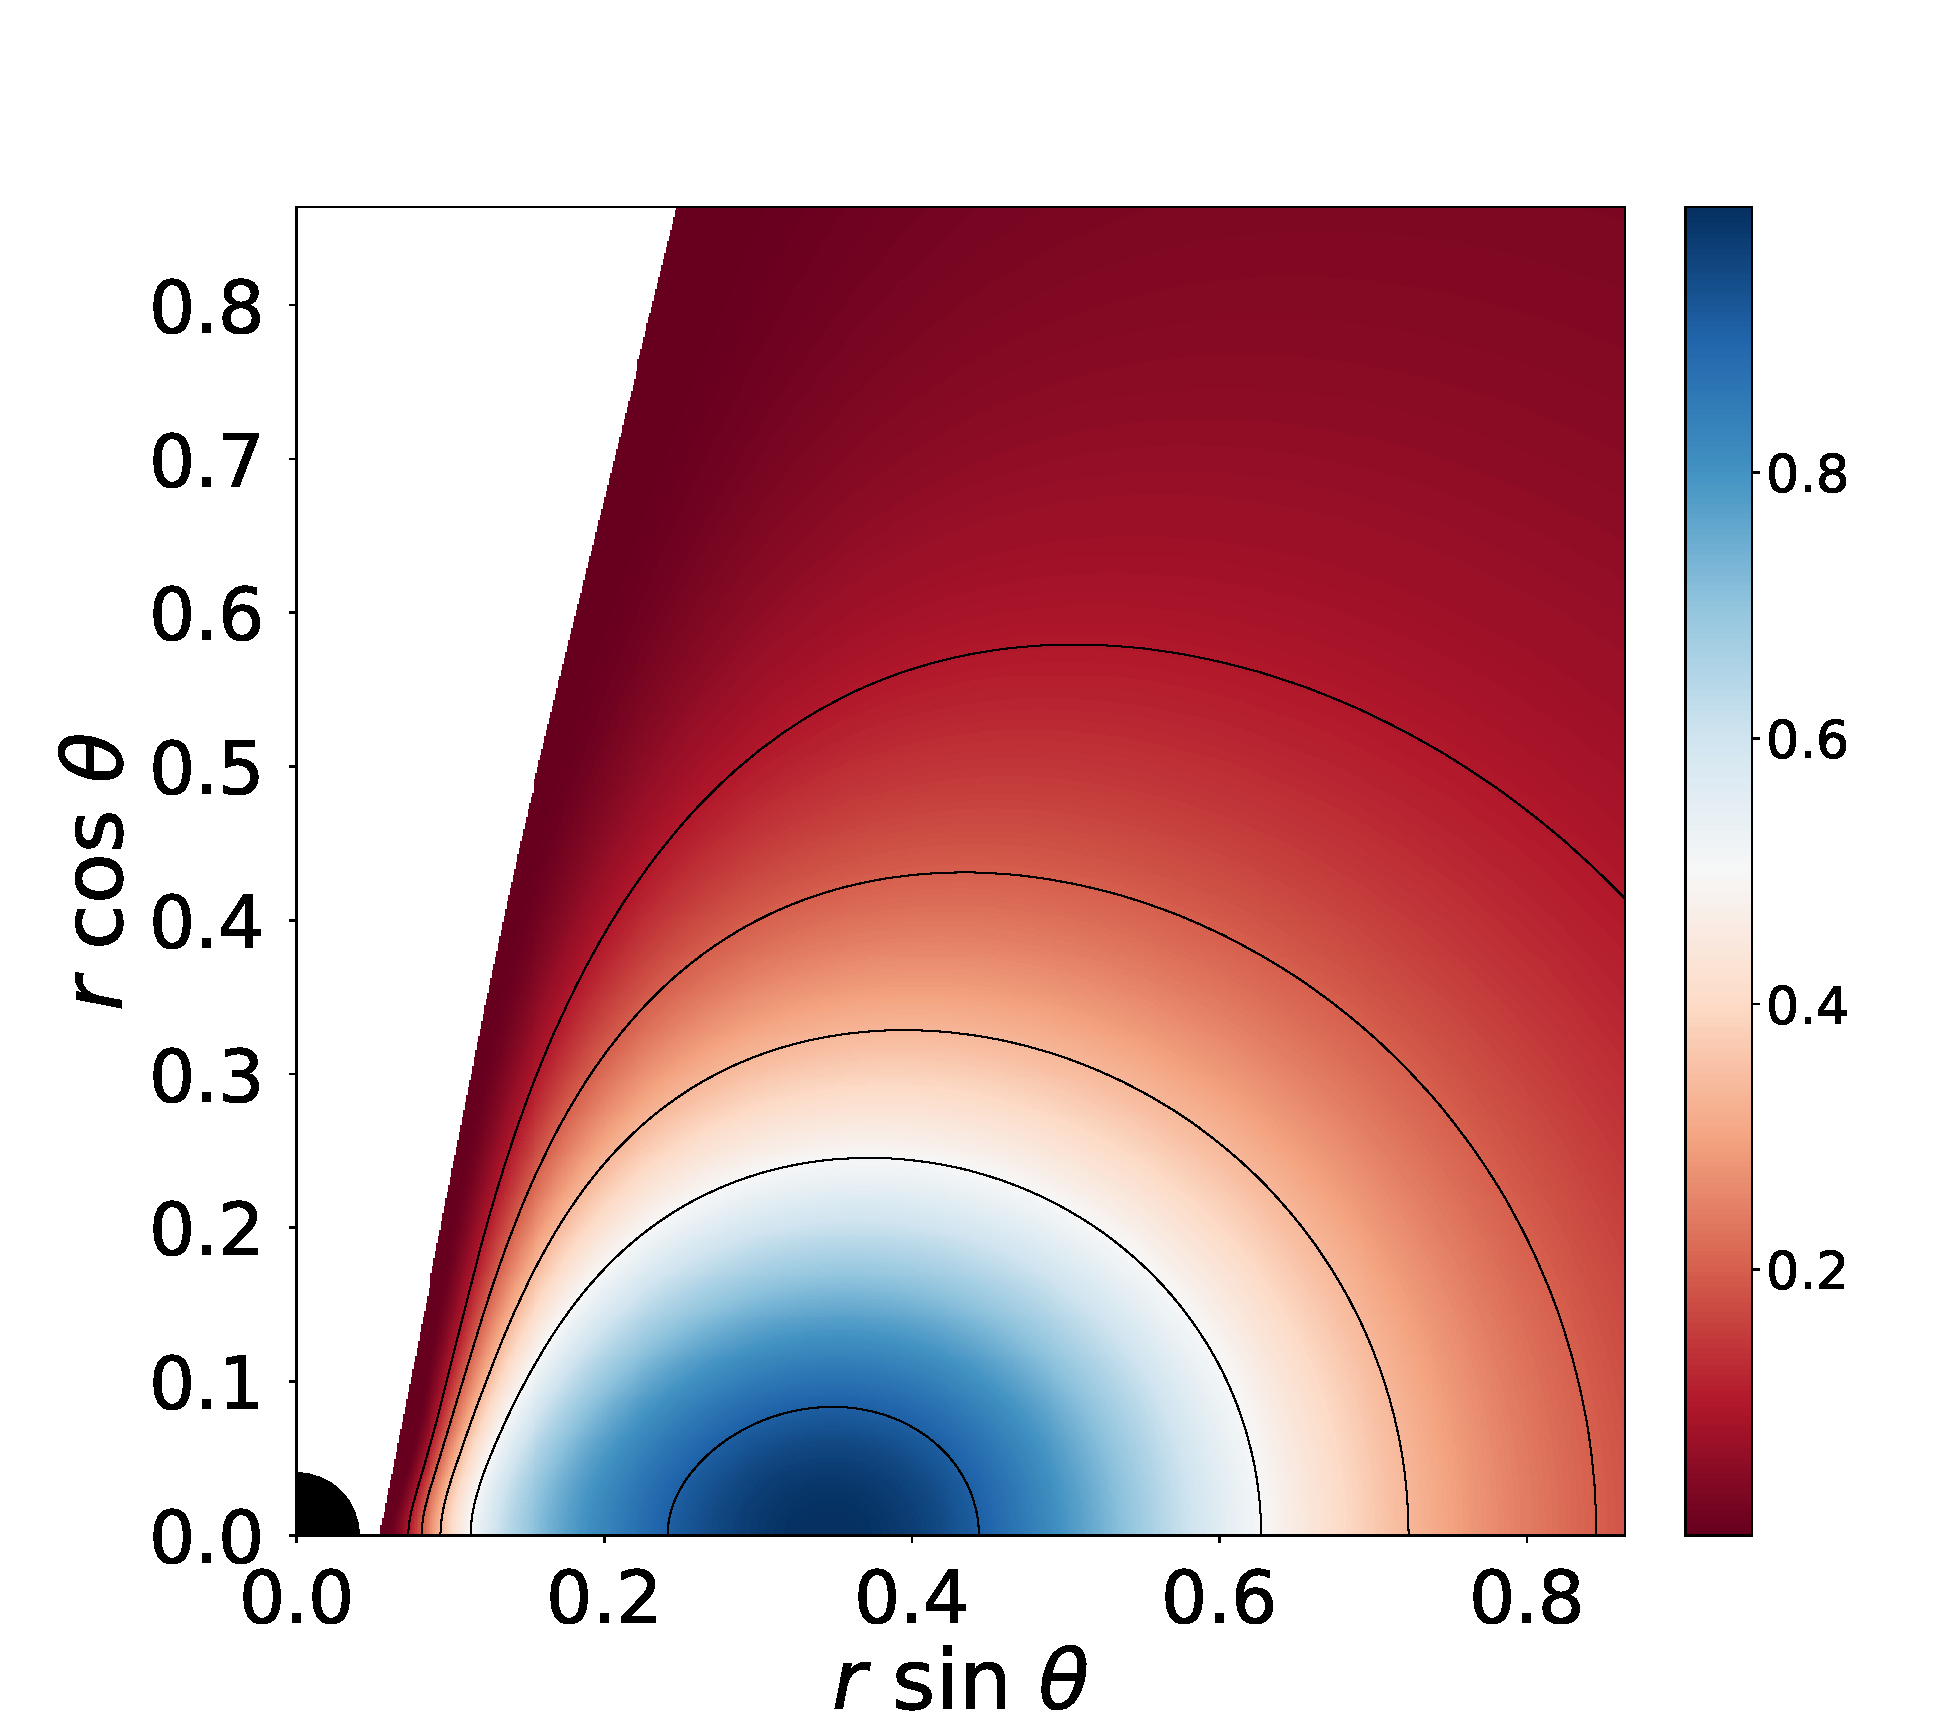
\includegraphics[scale=0.14]{figures/fig2_VII_10.pdf}
\hspace{-0.3cm}
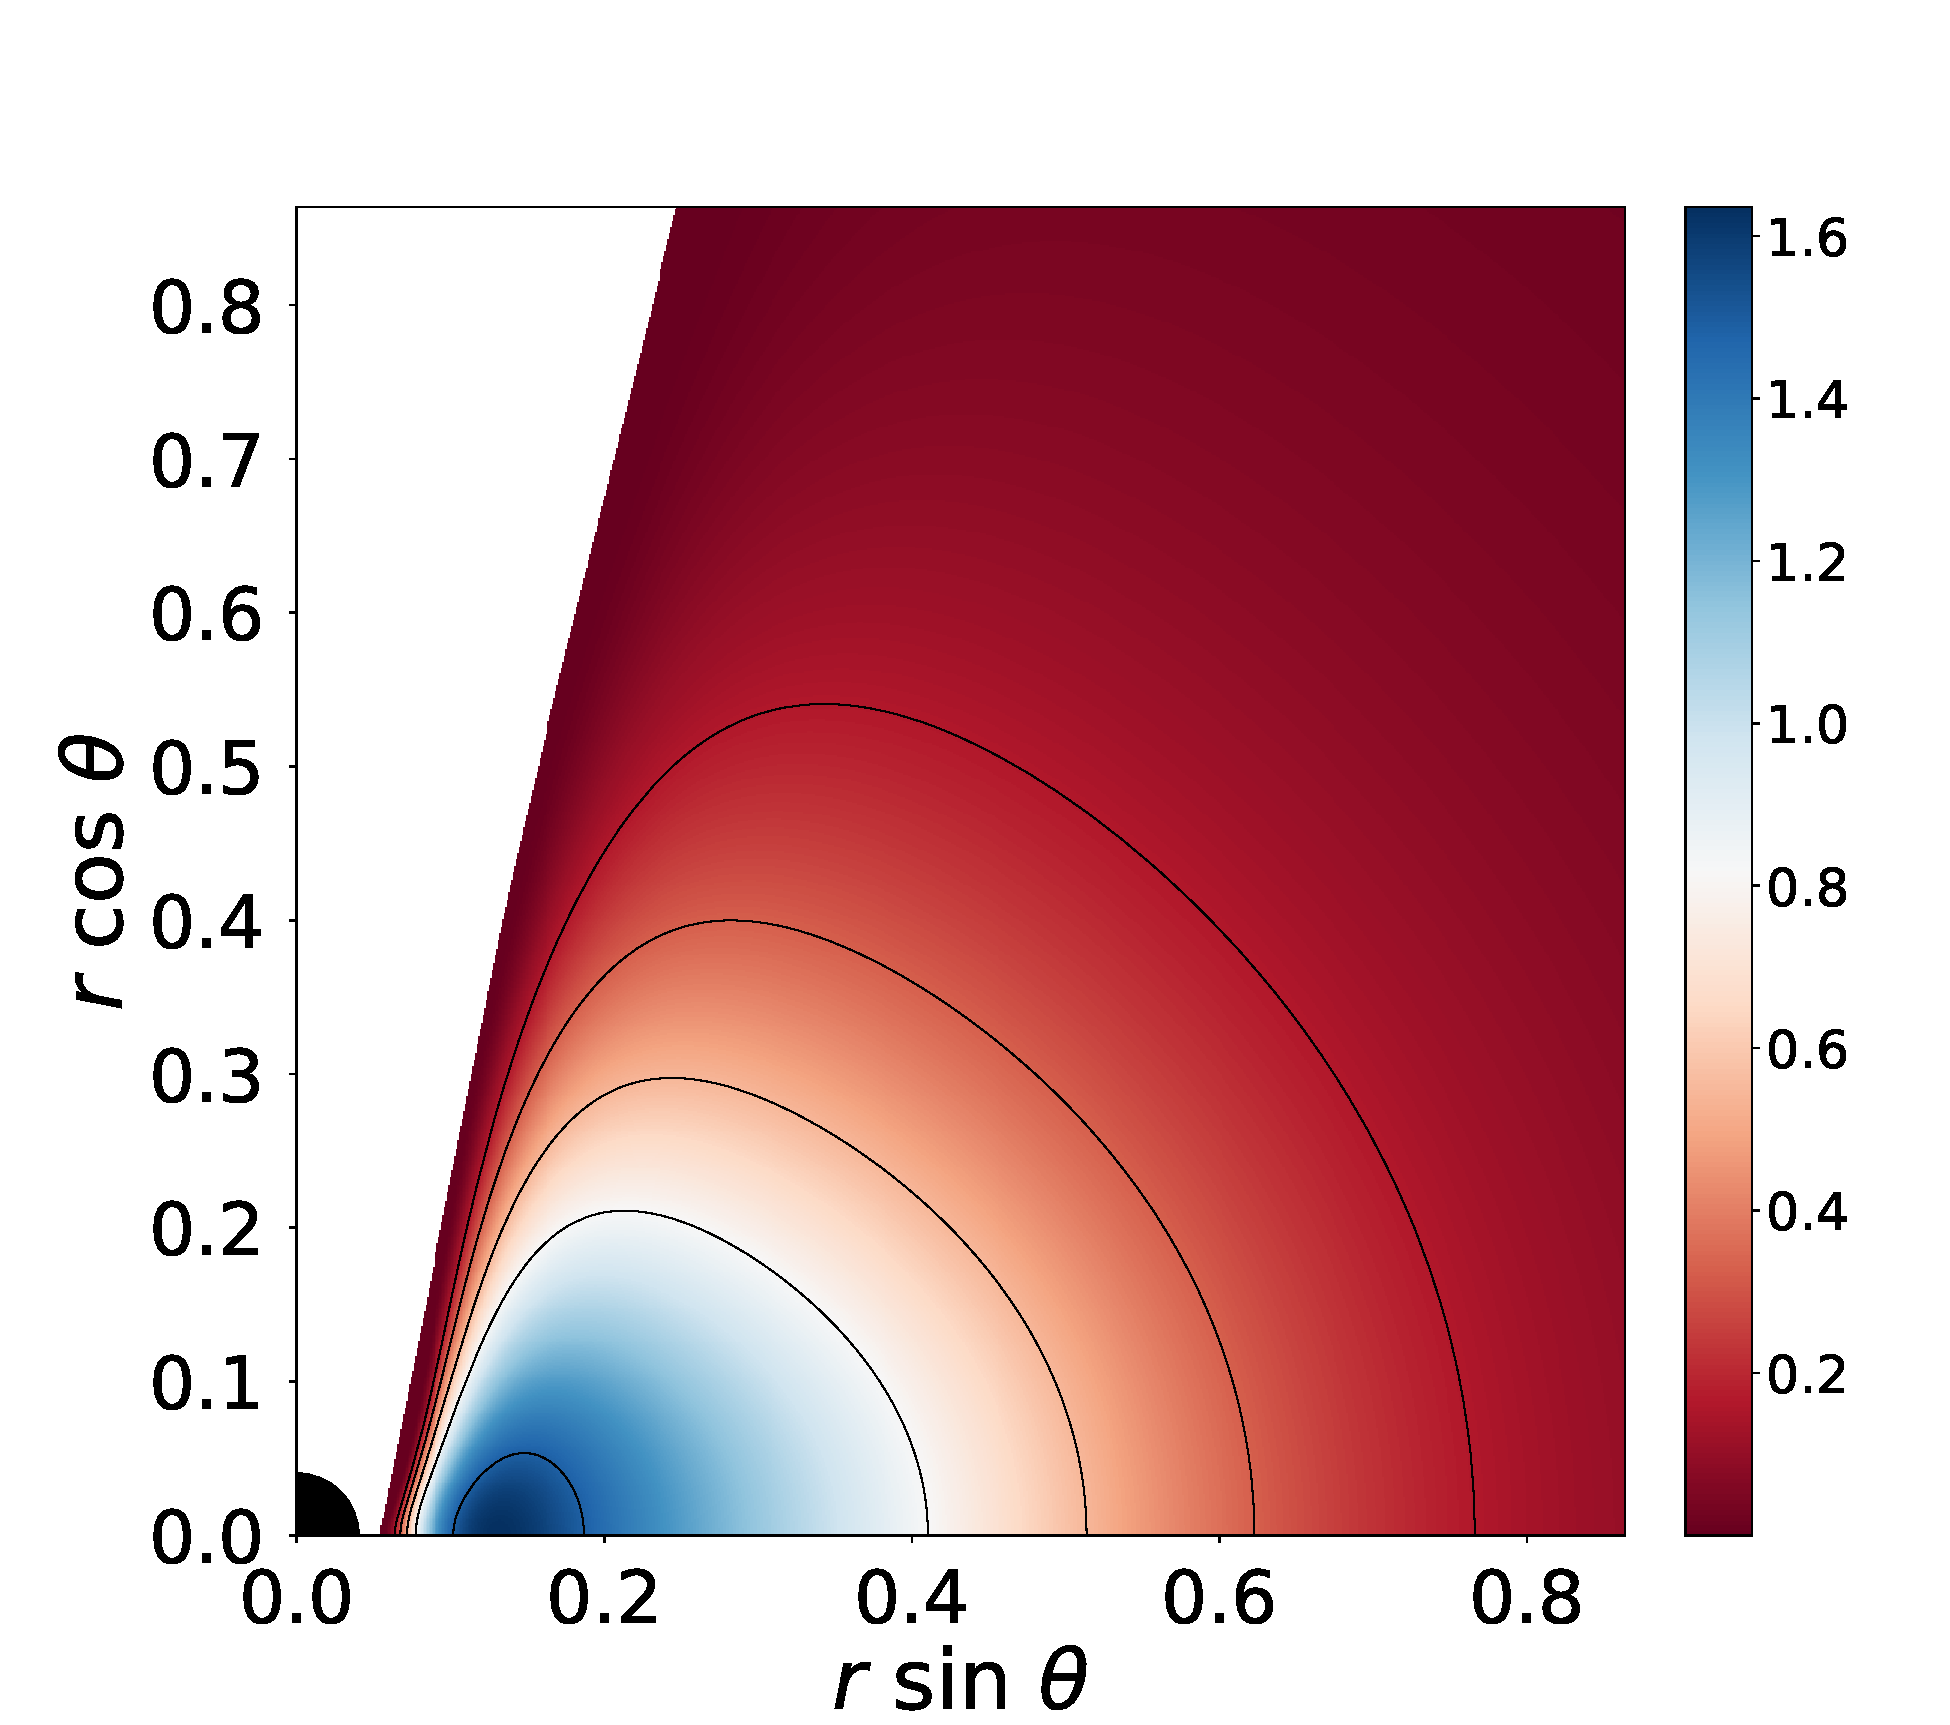
\includegraphics[scale=0.14]{figures/fig2_VII_1.pdf}
\hspace{-0.2cm}
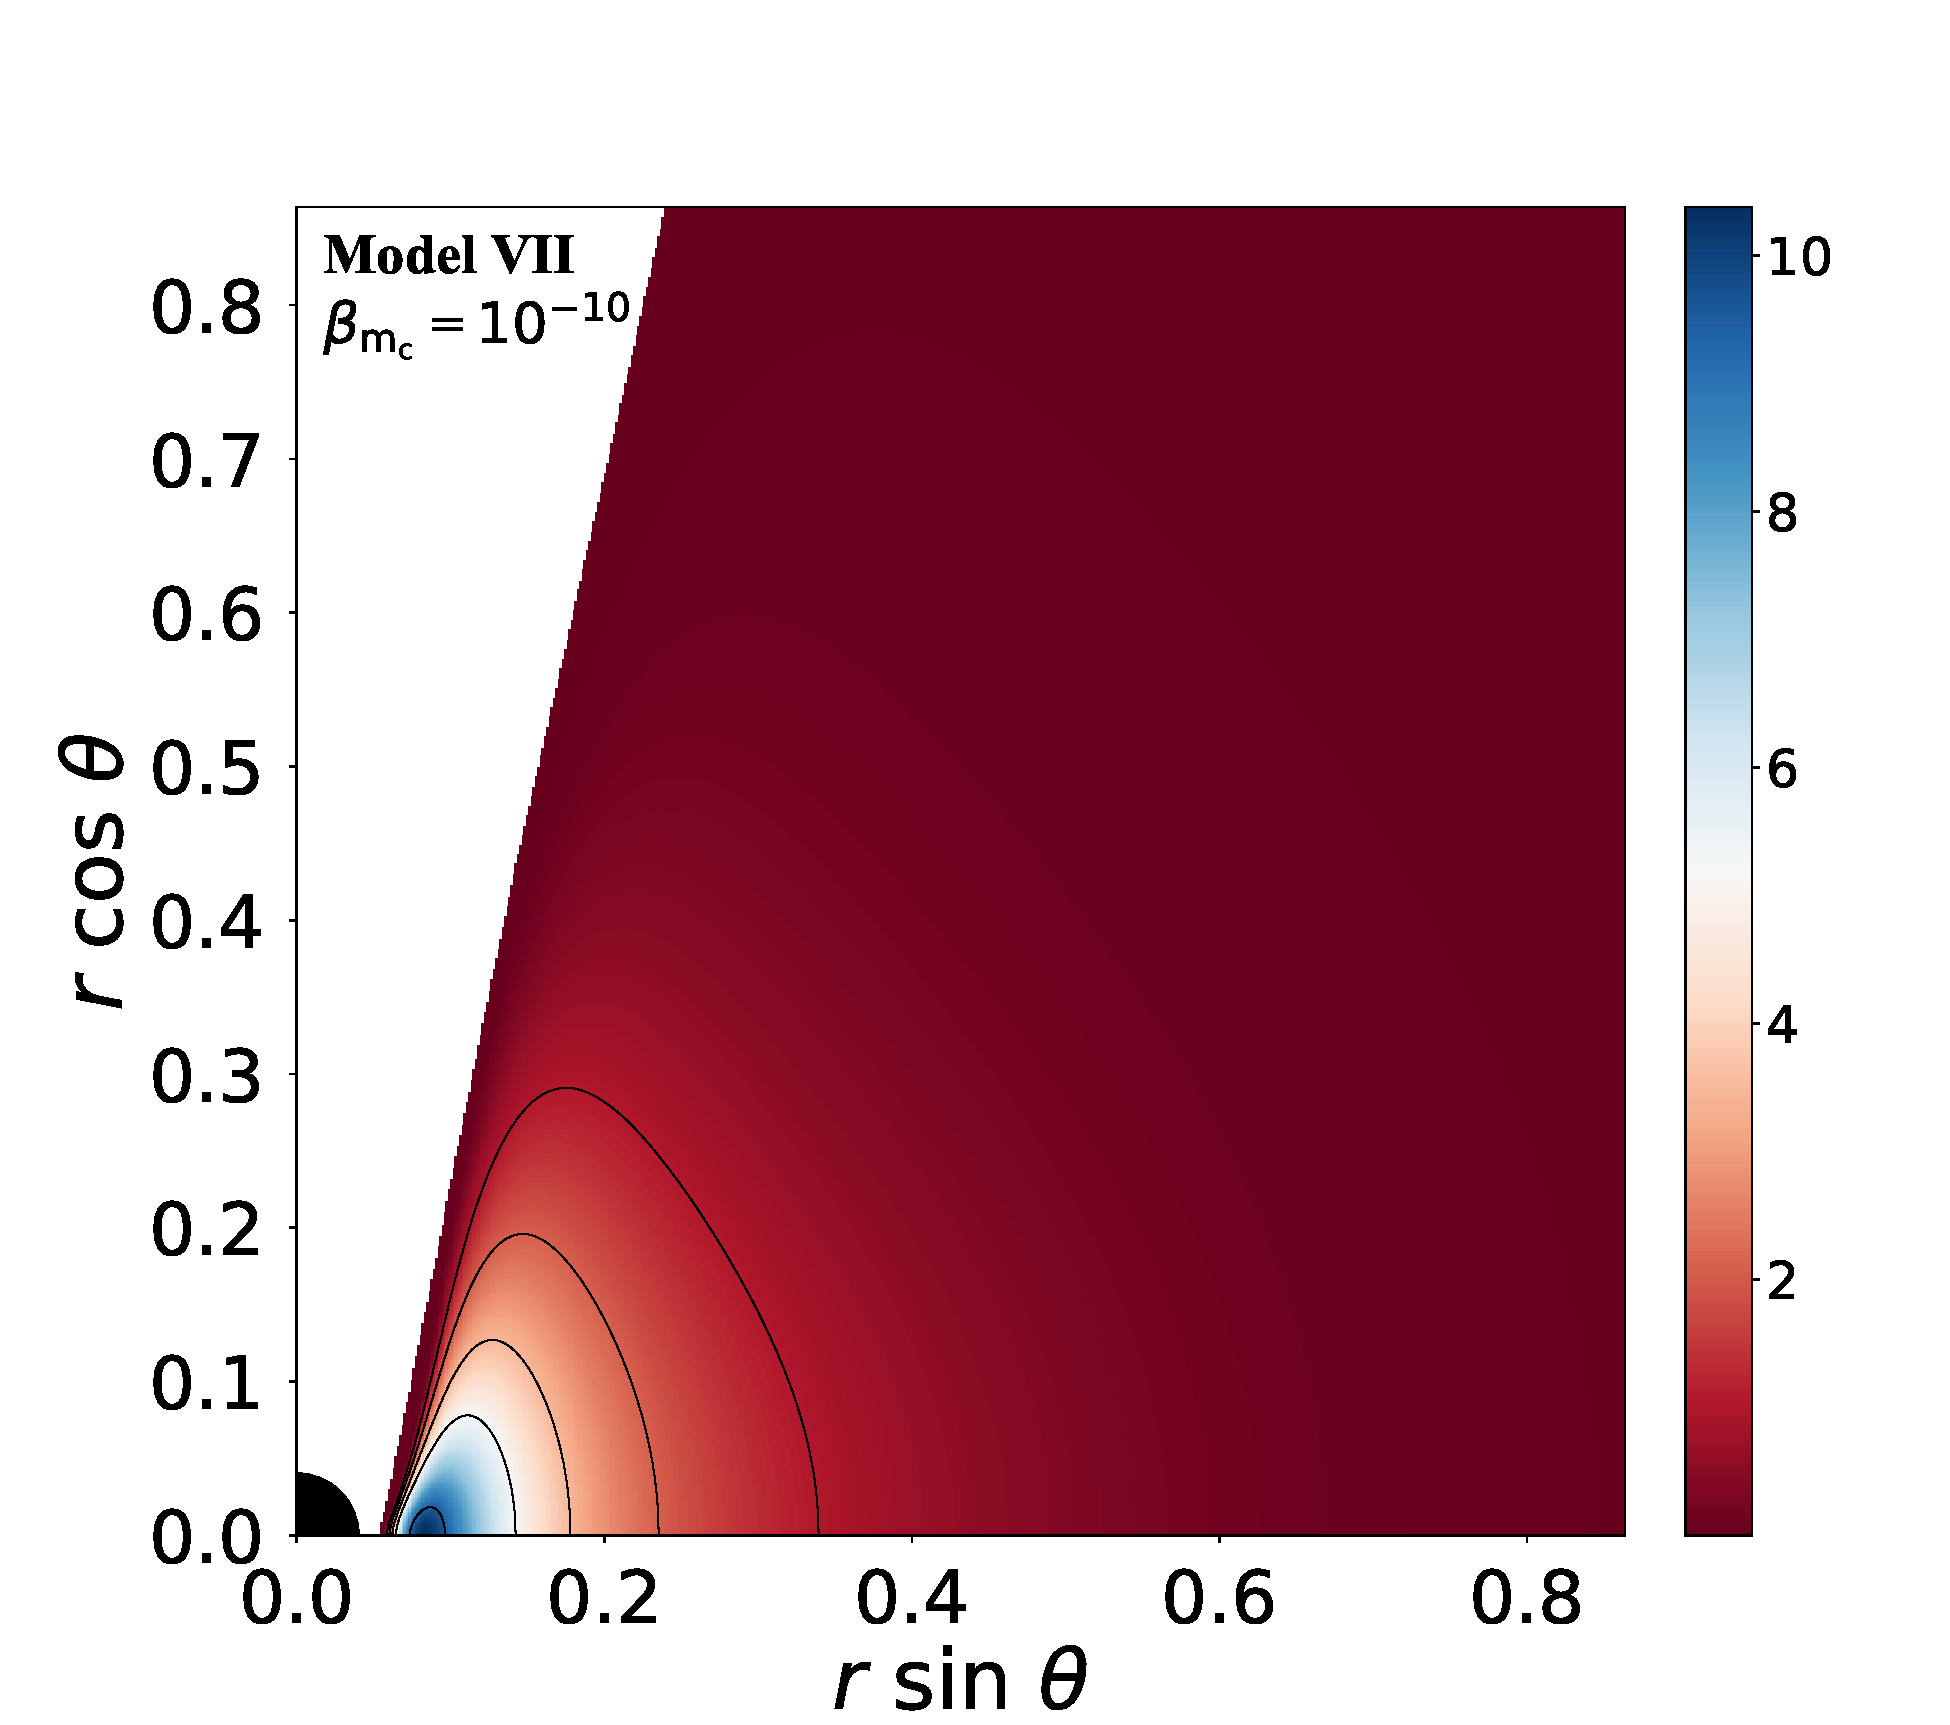
\includegraphics[scale=0.14]{figures/fig2_VII__10.pdf}
\hspace{-0.2cm}
\caption{Same as Fig.~\ref{models_I} but for the last three models of KBHsSH (V, VI, and VII).}
\label{models_II}
\end{figure*}

%%%%%%%%%%%%%%%%%%%%%%%%%%%%%%%%%%%%
\subsection{Distribution of angular momentum in the disk}
%%%%%%%%%%%%%%%%%%%%%%%%%%%%%%%%%%%%

Equilibrium models of thick disks around Kerr BHs are built assuming that the spacetime metric and the fluid fields are stationary and  axisymmetric (see, e.g.~\cite{Font:2002,Daigne:2004,Gimeno-Soler:2017} and references therein). For disks around KBHsSH we can follow the same approach as the metric ansatz given by Eq.~(\ref{metric}) is stationary and axisymmetric.

We start by introducing the specific angular momentum $l$ and the angular velocity $\Omega$ employing the standard definitions,
\begin{equation}
l = - \frac{u_{\phi}}{u_t}, \;\;\; \Omega = \frac{u^{\phi}}{u^t},
\end{equation}
where $u^{\mu}$ is the fluid four-velocity.
The relationship between $l$ and $\Omega$ is given by the equations
\begin{equation}
l = - \frac{\Omega g_{\phi\phi} + g_{t\phi}}{\Omega g_{t\phi} + g_{tt}}, \;\;\; \Omega = - \frac{l g_{tt} + g_{t\phi}}{l g_{t\phi} + g_{\phi\phi}},
\end{equation}
where we are assuming circular motion, i.e.~the four-velocity can be written as
\begin{equation}
u^{\mu} = (u^t, 0, 0, u^{\phi})\,.
\end{equation}

The approach we followed in~\cite{Gimeno-Soler:2017} for the angular momentum distribution of the disks was introduced by~\cite{Qian:2009}, and it is characterized by three free parameters, $\beta$, $\gamma$, and $\eta$ (see Eq.~(7) in~\cite{Gimeno-Soler:2017}). In this work, for simplicity and to reduce the ample space of parameters of the system, we consider a constant angular momentum distribution, $l(r,\theta) = \mathrm{const}$, which corresponds to setting $\beta=\gamma=0$ in~\cite{Gimeno-Soler:2017}. This choice also allows for the presence of a cusp (and hence matter accretion onto the black hole) and a centre. Following~\citep{Daigne:2004}, the specific value of the angular momentum corresponding to bound fluid elements ($-u_t<1$) is computed as the minimum of the following equation
\begin{equation}\label{eq:mb_ang_mom}
l^{\pm}_{\mathrm{b}}(r, \theta) = \frac{g_{t\phi} \pm \sqrt{ (g_{t\phi}^2-g_{tt}g_{\phi\phi})  (1+g_{tt}) } }{-g_{tt}}\,,
\end{equation}
where the plus sign corresponds to prograde orbits and the minus sign to retrograde orbits. Our convention is that the angular momentum of the BH is positive and the matter of the disk rotates in the positive (negative) direction of $\phi$ for a prograde (retrograde) disk.
Equation~(\ref{eq:mb_ang_mom}) is given by~\citep{Daigne:2004} for Kerr BHs, but it is valid for any stationary and axisymmetric spacetime. For prograde motion, the function has a minimum outside the event horizon. The location of this minimum corresponds with the marginally bound orbit $r_{\mathrm{mb}}$, and the angular momentum corresponds to the Keplerian angular momentum $l_{\mathrm{mb}}$ at that point. We show the proof of this statement in Appendix~\ref{ang_mom_appendix}.

%%%%%%%%%%%%%%%%
\subsection{Magnetized disks}
%%%%%%%%%%%%%%%%

To account for the magnetic field in the disks we use the procedure described by~\cite{Komissarov:2006,Montero:2007}. First, we write the equations of ideal general relativistic MHD as the following conservation laws, $\nabla_{\mu} T^{\mu\nu} = 0$, $\nabla_{\mu} \,^\ast F^{\mu\nu} = 0$, and 
$\nabla_{\mu} (\rho u^{\mu}) = 0$, 
where $\nabla_{\mu}$ is the covariant derivative and
\begin{equation}\label{eq:e-m_tensor}
T^{\mu\nu} = (\rho h + b^2)u^{\mu}u^{\nu} + (p + p_{\mathrm{m}})g^{\mu\nu} - b^{\mu}b^{\nu},
\end{equation}
is the energy-momentum tensor of a magnetized perfect fluid, $h$, $\rho$, $p$, and $p_{\mathrm{m}}$ being the fluid specific enthalpy, density, fluid pressure, and magnetic pressure, respectively, the latter defined as $p_{\mathrm{m}} = b^2/2$. The ratio of fluid pressure to magnetic pressure defines the magnetization parameter $\beta_{\mathrm{m}} = p/p_{\mathrm{m}}$.
Moreover, $^\ast F^{\mu\nu} = b^{\mu}u^{\nu} - b^{\nu}u^{\mu}$ is the (dual of the) Faraday tensor relative to an observer with 
four-velocity $u^{\mu}$, and $b^{\mu}$ is the magnetic field in that frame, with
$b^2=b^{\mu}b_{\mu}$ (see~\cite{Anton:2006} for further details). Assuming the magnetic field is purely azimuthal, i.e.~$b^r = b^{\theta} = 0$,
and taking into account that the flow is stationary and axisymmetric, the conservation of the current density and of the Faraday tensor follow. Contracting the divergence of Eq.~\eqref{eq:e-m_tensor} with the projection tensor $h^{\alpha}_{\,\,\beta} = \delta^{\alpha}_{\,\,\beta} + u^{\alpha}u_{\beta}$, we arrive at
\begin{equation}
(\rho h + b^2)u_{\nu}\partial_i u^{\nu} + \partial_i\left(p + \frac{b^2}{2}\right) - b_{\nu}\partial_i b^{\nu}=0\,,
\end{equation}
where $i = r, \theta$. This equation can be rewritten in terms of the specific angular momentum $l$ and of the angular velocity $\Omega$, 
\begin{equation}\label{eq:diff_ver}
\partial_i(|\ln u_t|) - \frac{\Omega \partial_i l}{1-l\Omega} + \frac{\partial_i p}{\rho h} + \frac{\partial_i(\mathcal{L}b^2)}{2\mathcal{L}\rho h} = 0\,,
\end{equation}
where $\mathcal{L} = g_{t\phi}^2 - g_{tt}g_{\phi\phi}$.

To integrate Eq.~\eqref{eq:diff_ver} we need to assume an equation of state (EOS). We assume a polytropic EOS of the form
\begin{equation}\label{eq:eos_fluid}
p = K \rho^{\Gamma},
\end{equation}
with $K$ and $\Gamma$ constants.
 By introducing the definitions $\tilde{p}_{\mathrm{m}} = \mathcal{L} p_{\mathrm{m}}$, $w = \rho h$ and $\tilde{w} = \mathcal{L} (w)$, we can write equations equivalent to Eq.~\eqref{eq:eos_fluid} for both $\tilde{p}_{\mathrm{m}}$ and $p_{\mathrm{m}}$
\begin{eqnarray}
\label{eq:eos_mag_tilde}
\tilde{p}_{\mathrm{m}} &=& K_{\rm m} \tilde{w}^q,
\\
p_{\mathrm{m}} &=& K_{\rm m} \mathcal{L}^{q-1} (\rho h)^q,
\end{eqnarray}
where $K_{\rm m}$ and $q$ are constants. Then we can integrate Eq.~\eqref{eq:diff_ver} as
\begin{equation}\label{eq:final}
W - W_{\mathrm{in}} + \ln \left(1 + \frac{\Gamma K}{\Gamma +1}\rho^{\Gamma -1}\right) + \frac{q}{q-1}K_{\rm m}(\mathcal{L}\rho h)^{q-1}=0,
\end{equation}
where $W \equiv \ln |u_t|$ stands for the (gravitational plus centrifugal) potential and $W_{\mathrm{in}}$ is the potential at the inner edge of the disk.

We can also define the total energy density for the torus, $\rho_{\mathrm{T}}=-T^t_t + T^i_i$, and for the scalar field, $\rho_{\mathrm{SF}}=-(T_{\mathrm{SF}})^t_t + (T_{\mathrm{SF}})^i_i$. These are given by
\begin{eqnarray}\label{eq:torus_energy_density}
\rho_{\mathrm{T}} &=&  \frac{\rho h (g_{\phi\phi} - g_{tt} l^2)}{g_{\phi\phi} + 2 g_{t\phi} l + g_{tt} l^2} + 2 (p + p_{\mathrm{m}}),
\\
\rho_{\mathrm{SF}} &=&  2 \left(\frac{2 e^{-2 F_0} w (w-m W)}{N} - \mu^2\right) \phi^2.
\end{eqnarray}
Using these expressions, we can compute the total gravitational mass of the torus and the scalar field as the following expression
\begin{equation}\label{eq:mass_integral}
\mathcal{M} = \int  \rho \sqrt{-g}\,\mathrm{d}^3x\,,
\end{equation}
where $g$ is the determinant of the metric tensor and $\rho\equiv \rho_{\mathrm{T}}, \rho_{\mathrm{SF}}$.

In this work we take an approach to construct the magnetized disks different to the one proposed by~\citep{Komissarov:2006} and used by~\cite{Vincent:2016} for building disks around KBHsSH. As noted by~\cite{Gimeno-Soler:2017}, the approach of~\citep{Komissarov:2006} implicitly assumes that the specific enthalpy of the fluid is close to unity ($w = \rho h \simeq \rho$). This means that the polytropic EOS Eq.~\eqref{eq:eos_fluid} can be written as $p = K w^{\Gamma}$ (see Eq.~(27) of~\cite{Komissarov:2006}). We do not make this assumption here. To better understand the differences between these two approaches, we consider their behaviour in two limiting cases, namely the non-magnetised case and the extremely magnetised case.

For the former, we can rewrite Eq.~\eqref{eq:final} in the limiting case of $\beta_{\mathrm{m_c}} \rightarrow \infty$ ($K_{\rm m} \rightarrow 0$) as
\begin{equation}
W - W_{\mathrm{in}} + \ln \left(1 + \frac{\Gamma K}{\Gamma +1}\rho^{\Gamma -1}\right) = 0.
\end{equation}
Then, we can solve this equation for the specific enthalpy
\begin{equation}\label{eq:rel_non_mag_enth}
h = e^{W_{\mathrm{in}} - W}.
\end{equation}
Now, we want to obtain an analogous equation for the $h \simeq 1$ case. We start by considering Eq.~(20) of~\cite{Gimeno-Soler:2017} and taking the limit $\beta_{\mathrm{m_c}} \rightarrow \infty$ (in this equation, this means $K_{\mathrm{m}} \rightarrow 0$), to obtain
\begin{equation}
W - W_{\mathrm{in}} + \frac{\Gamma K}{\Gamma +1}w^{\Gamma -1}.
\end{equation}
If we consider the $h \simeq 1$ approximmation, we can use the definition of $h$ and solve the equation to arrive at
\begin{equation}\label{eq:non_rel_non_mag_enth}
h = 1 + (W_{\mathrm{in}} - W).
\end{equation}
If we compare both results, we can see that Eq.~\eqref{eq:non_rel_non_mag_enth} is the first-order Taylor series expansion of Eq.~\eqref{eq:rel_non_mag_enth} for a sufficiently small value of $W_{\mathrm{in}} - W$.

\begin{figure*}
\centering
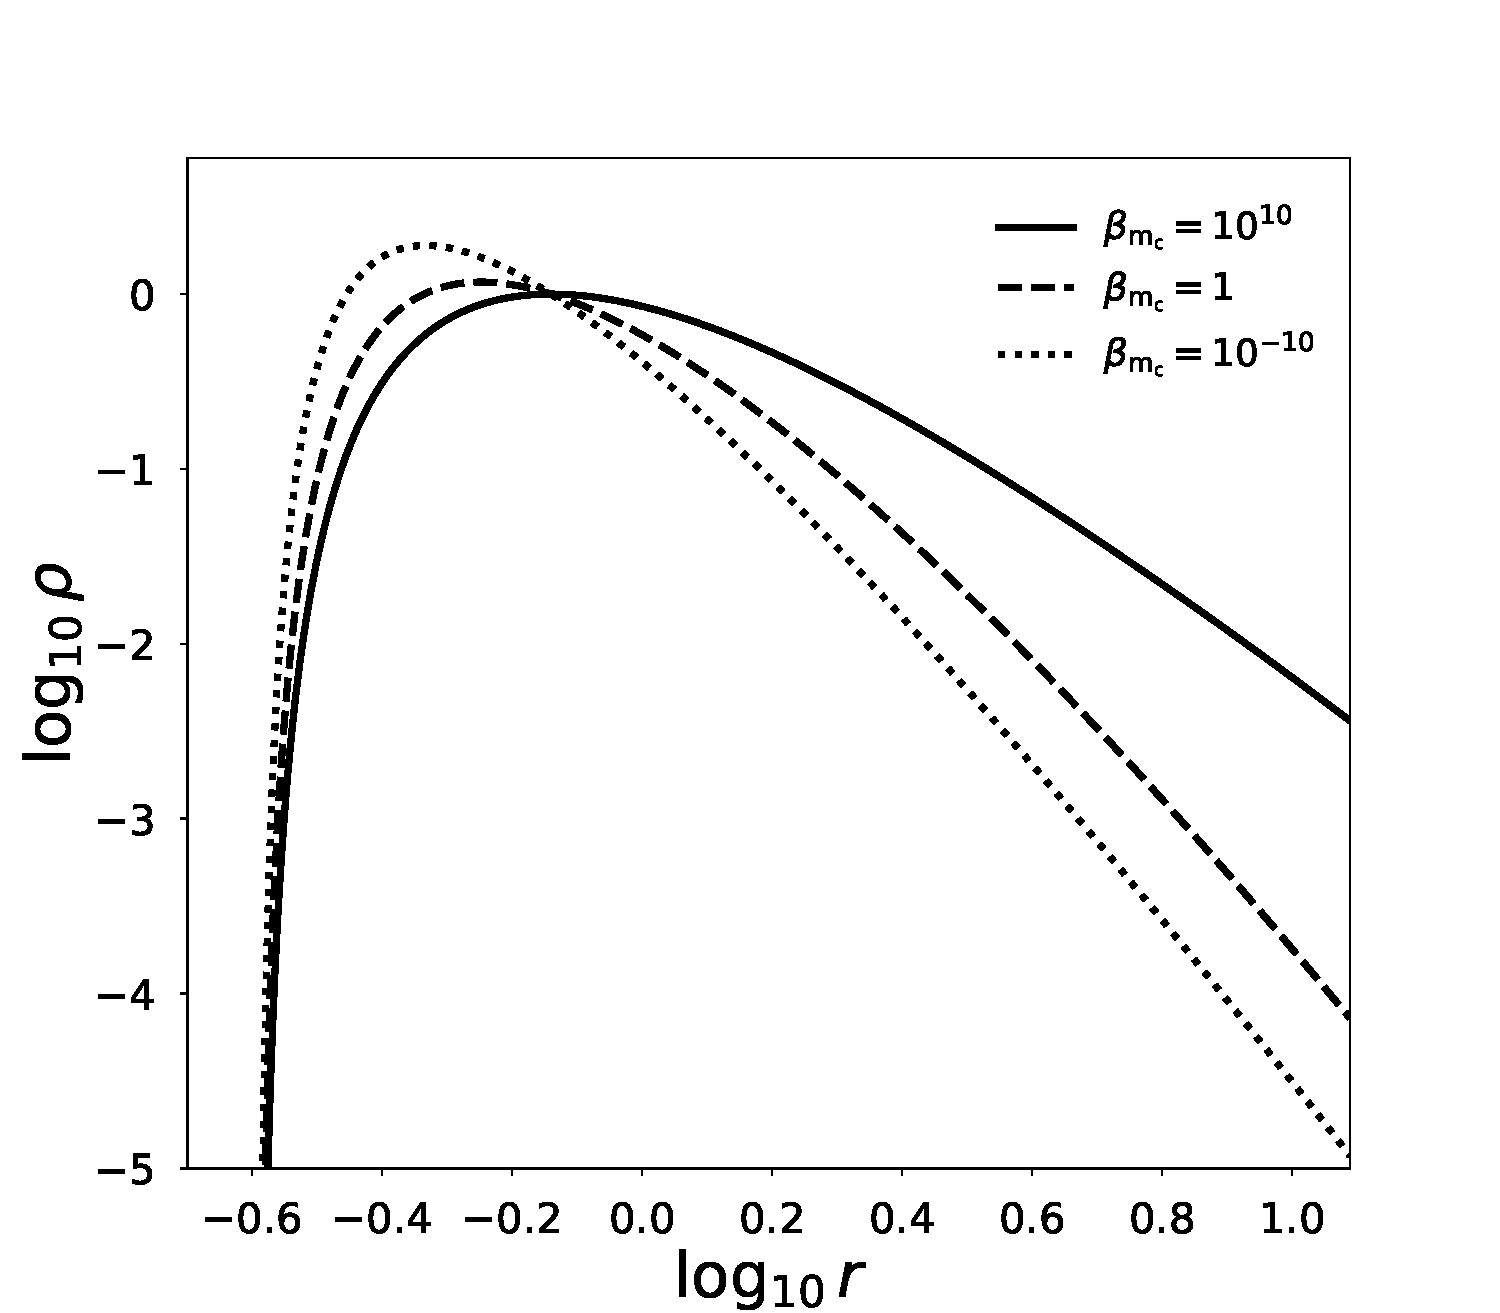
\includegraphics[scale=0.37]{figures/radial_log_rho_model_I.pdf}
\hspace{-0.6cm}
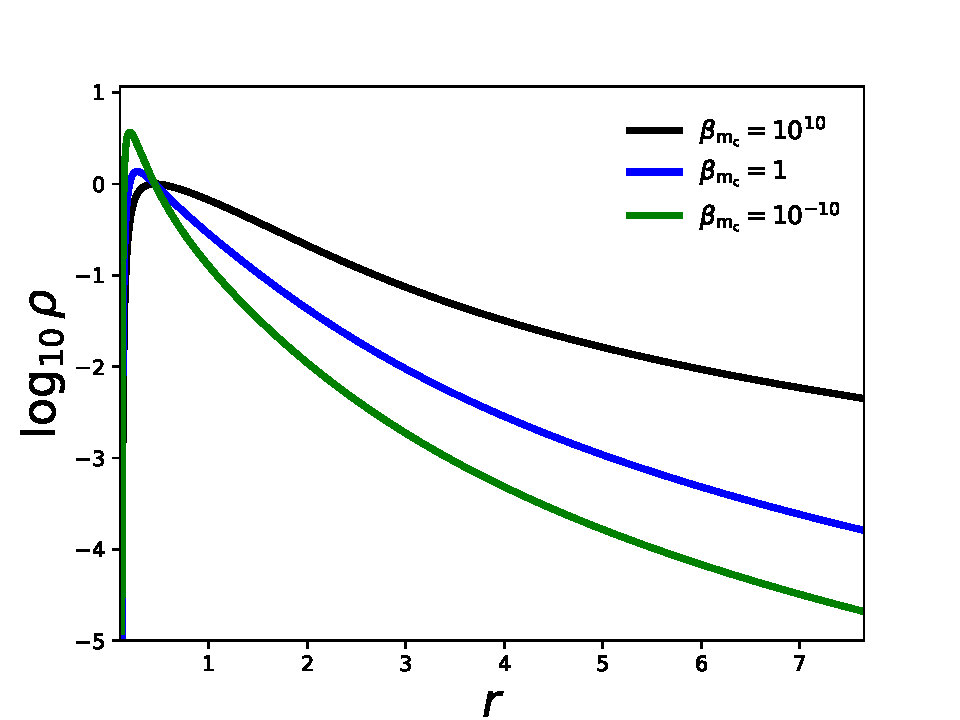
\includegraphics[scale=0.37]{figures/radial_log_rho_model_IV.pdf}
\hspace{-0.6cm}
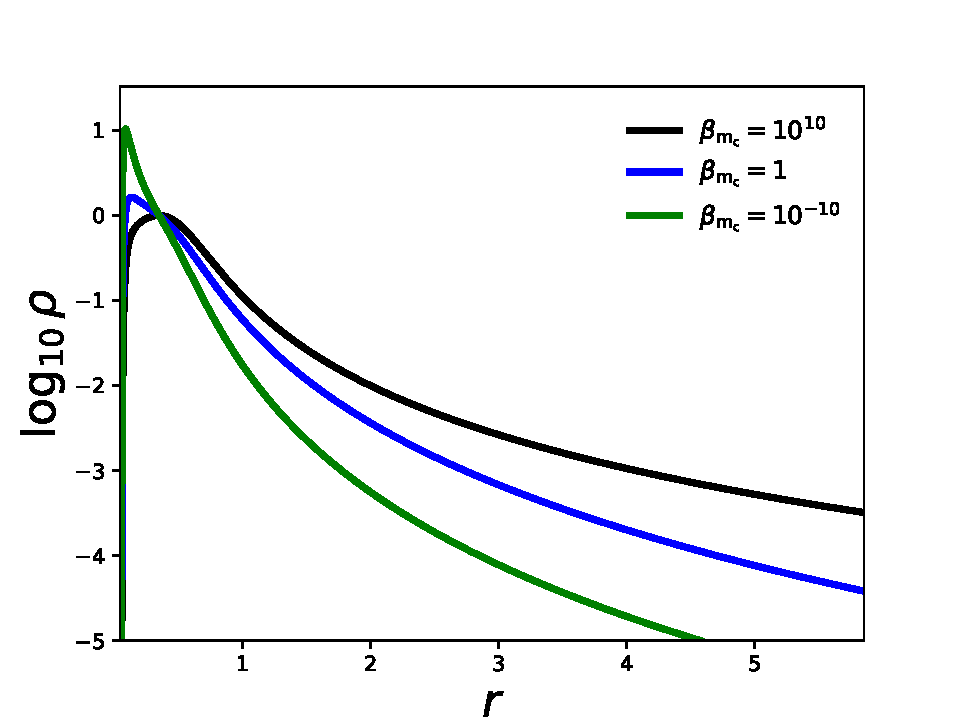
\includegraphics[scale=0.37]{figures/radial_log_rho_model_VII.pdf}
\hspace{-0.6cm}
\caption{Size of the disks. Effects of the magnetisation on the radial profiles of the logarithm of the density at the equatorial plane for different KBHsSH models. From left to right we show model I, IV, and VII, respectively.}
\label{radial_profiles_HBH}
\end{figure*}

For the extremely magnetised case, we consider again Eq.~\eqref{eq:final} and Eq.~(20) of~\cite{Gimeno-Soler:2017}, but this time around we take $\beta_{\mathrm{m_c}} \rightarrow 0$ ($K \rightarrow 0$). This yields the same result for both equations
\begin{equation}
W - W_{\mathrm{in}} + \frac{q}{q-1}K_{\rm m}(\mathcal{L}\rho h)^{q-1}=0.
\end{equation}
In addition, we could consider the expression for the specific enthalpy in terms of the density $h = 1 + \frac{K\Gamma\rho^{\Gamma-1}}{\Gamma - 1}$ to 
see that we will have $h \rightarrow 1$. This shows that, for the extremely magnetised limit, the two approaches coincide.

Taking into account these two limits we can obtain the range of validity of the $h \simeq 1$ approximation: As magnetised disks exist between the two considered cases, for disks with a sufficiently small value of the potential well, $\Delta W \equiv W_{\mathrm{in}} - W_{\mathrm{c}}$, the $h \simeq 1$ approximation is valid. On the contrary, if the value of $\Delta W$ is large enough, the approximation does not hold even for disks with a fairly low value of magnetisation.

\begin{figure*}
\centering
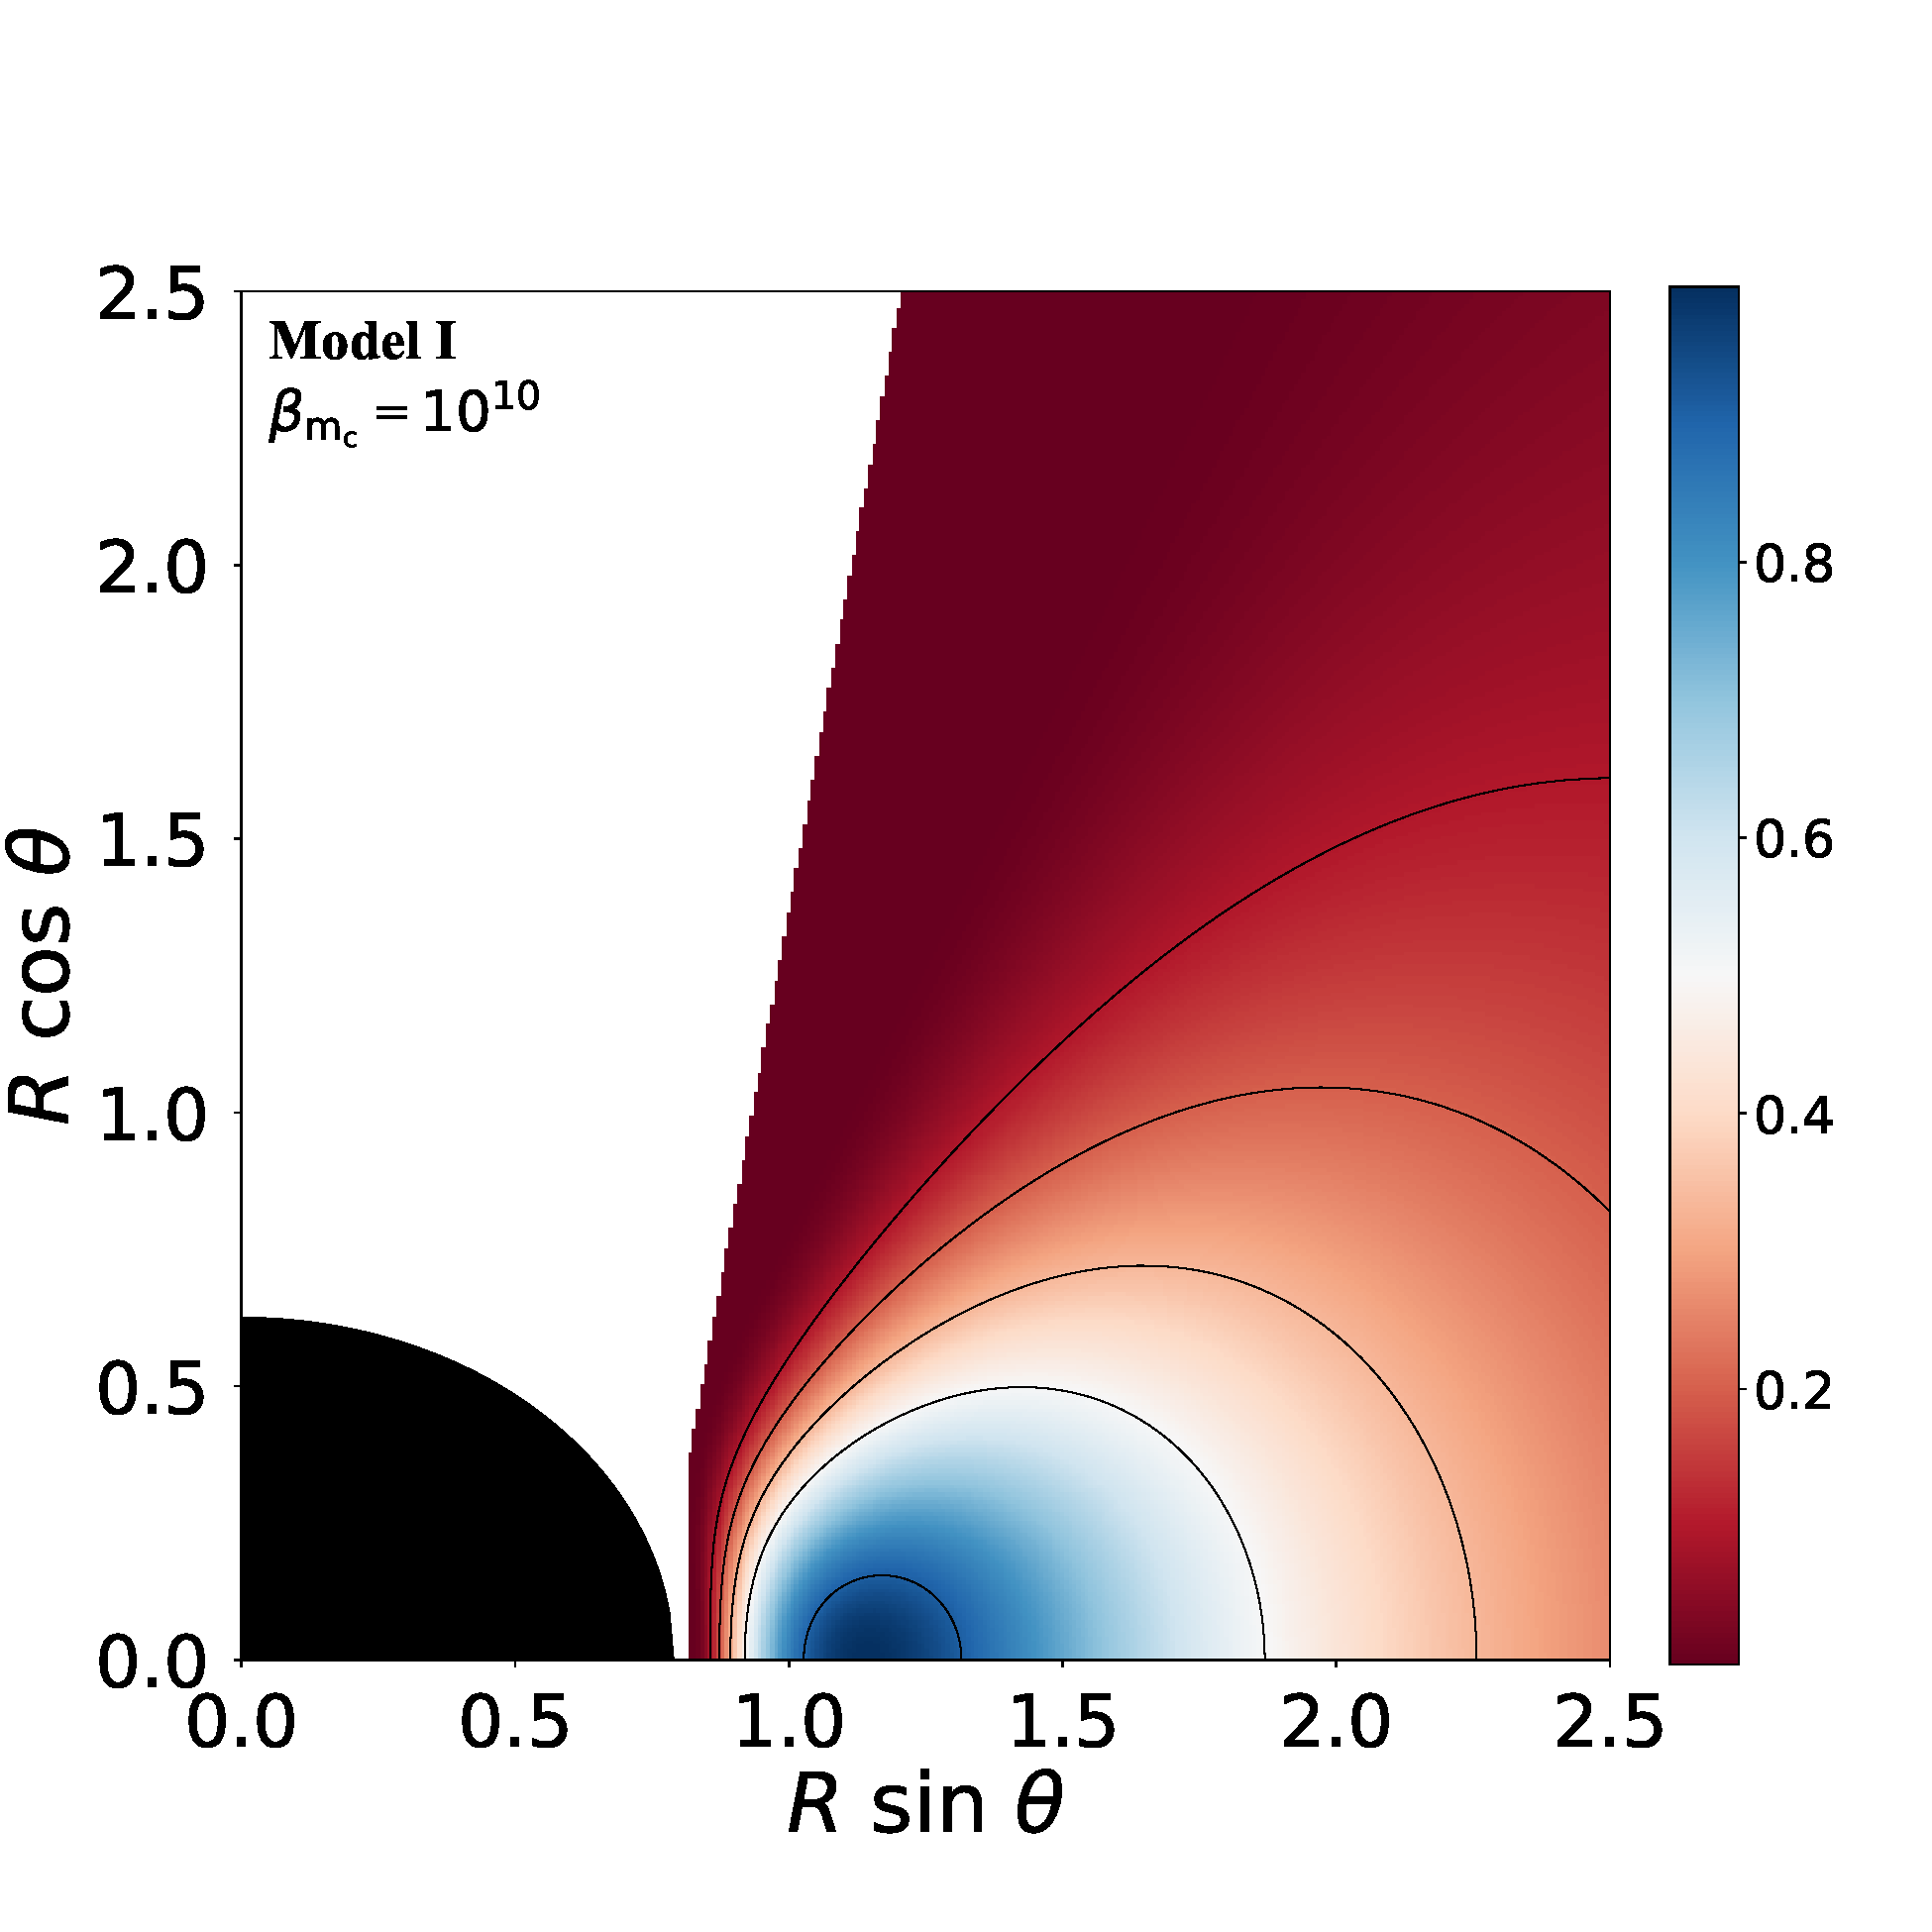
\includegraphics[scale=0.14]{figures/fig3_I_10.pdf}
\hspace{-0.3cm}
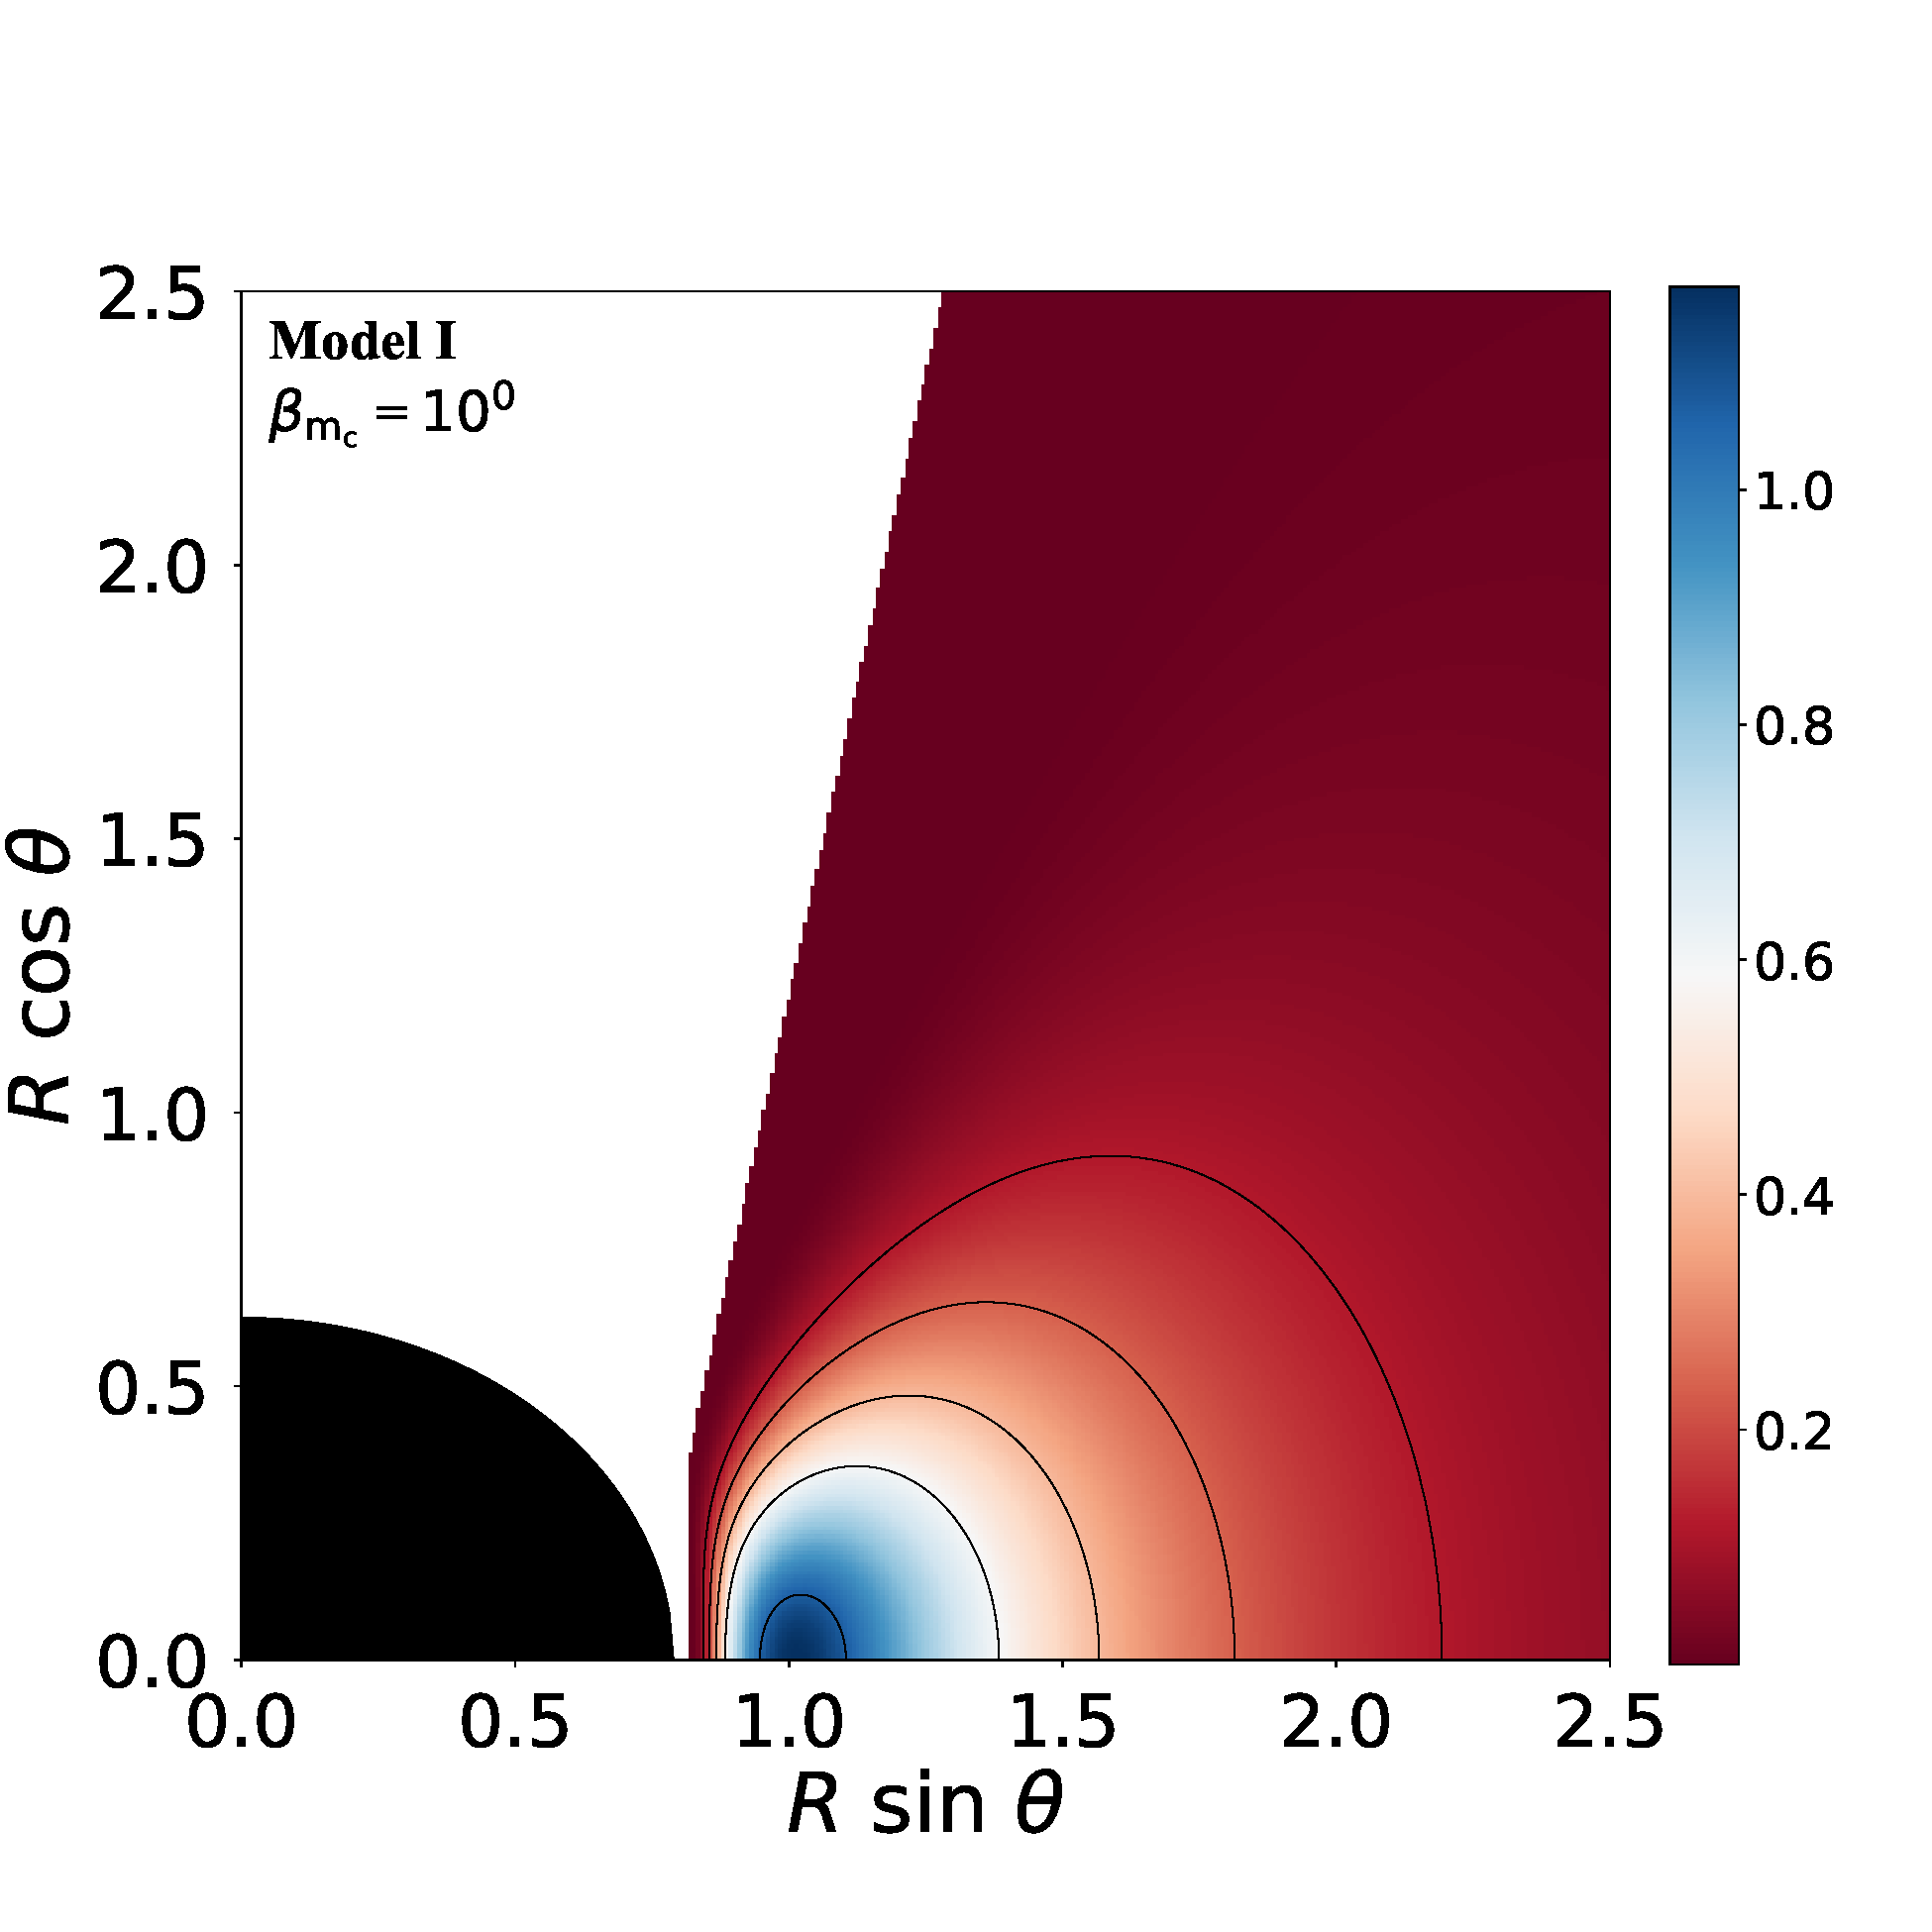
\includegraphics[scale=0.14]{figures/fig3_I_1.pdf}
\hspace{-0.2cm}
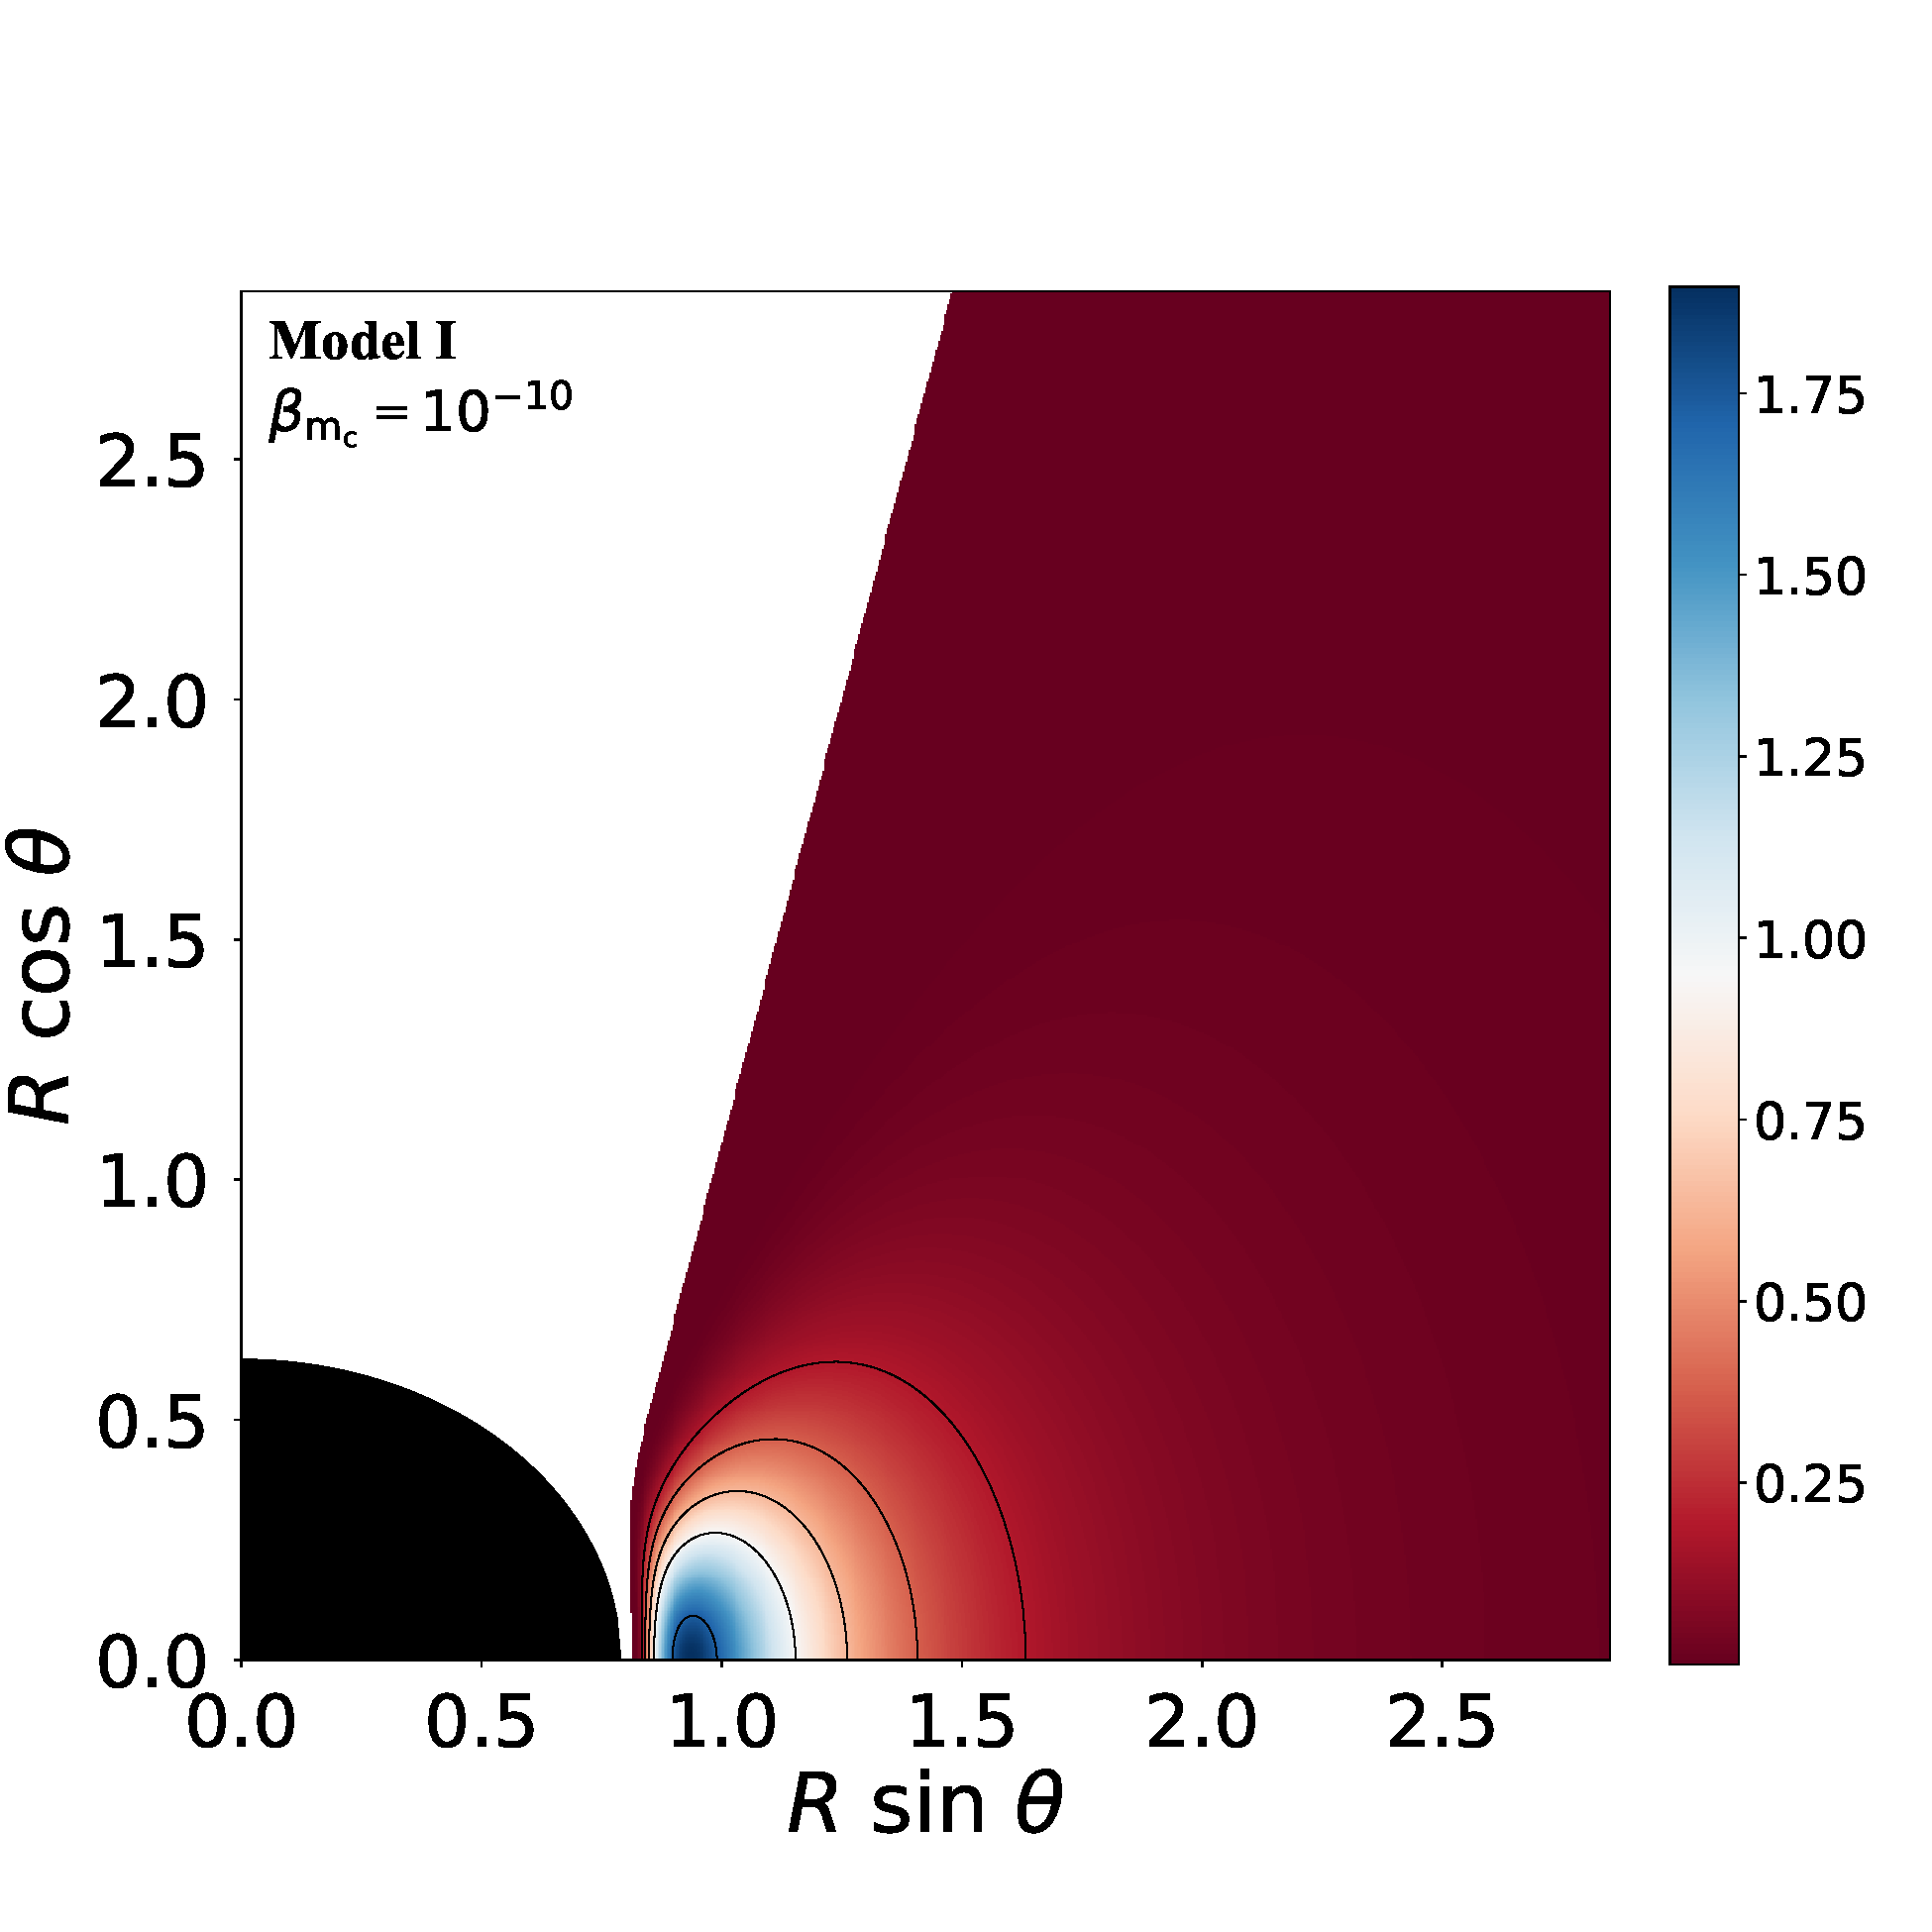
\includegraphics[scale=0.14]{figures/fig3_I__10.pdf}
\\
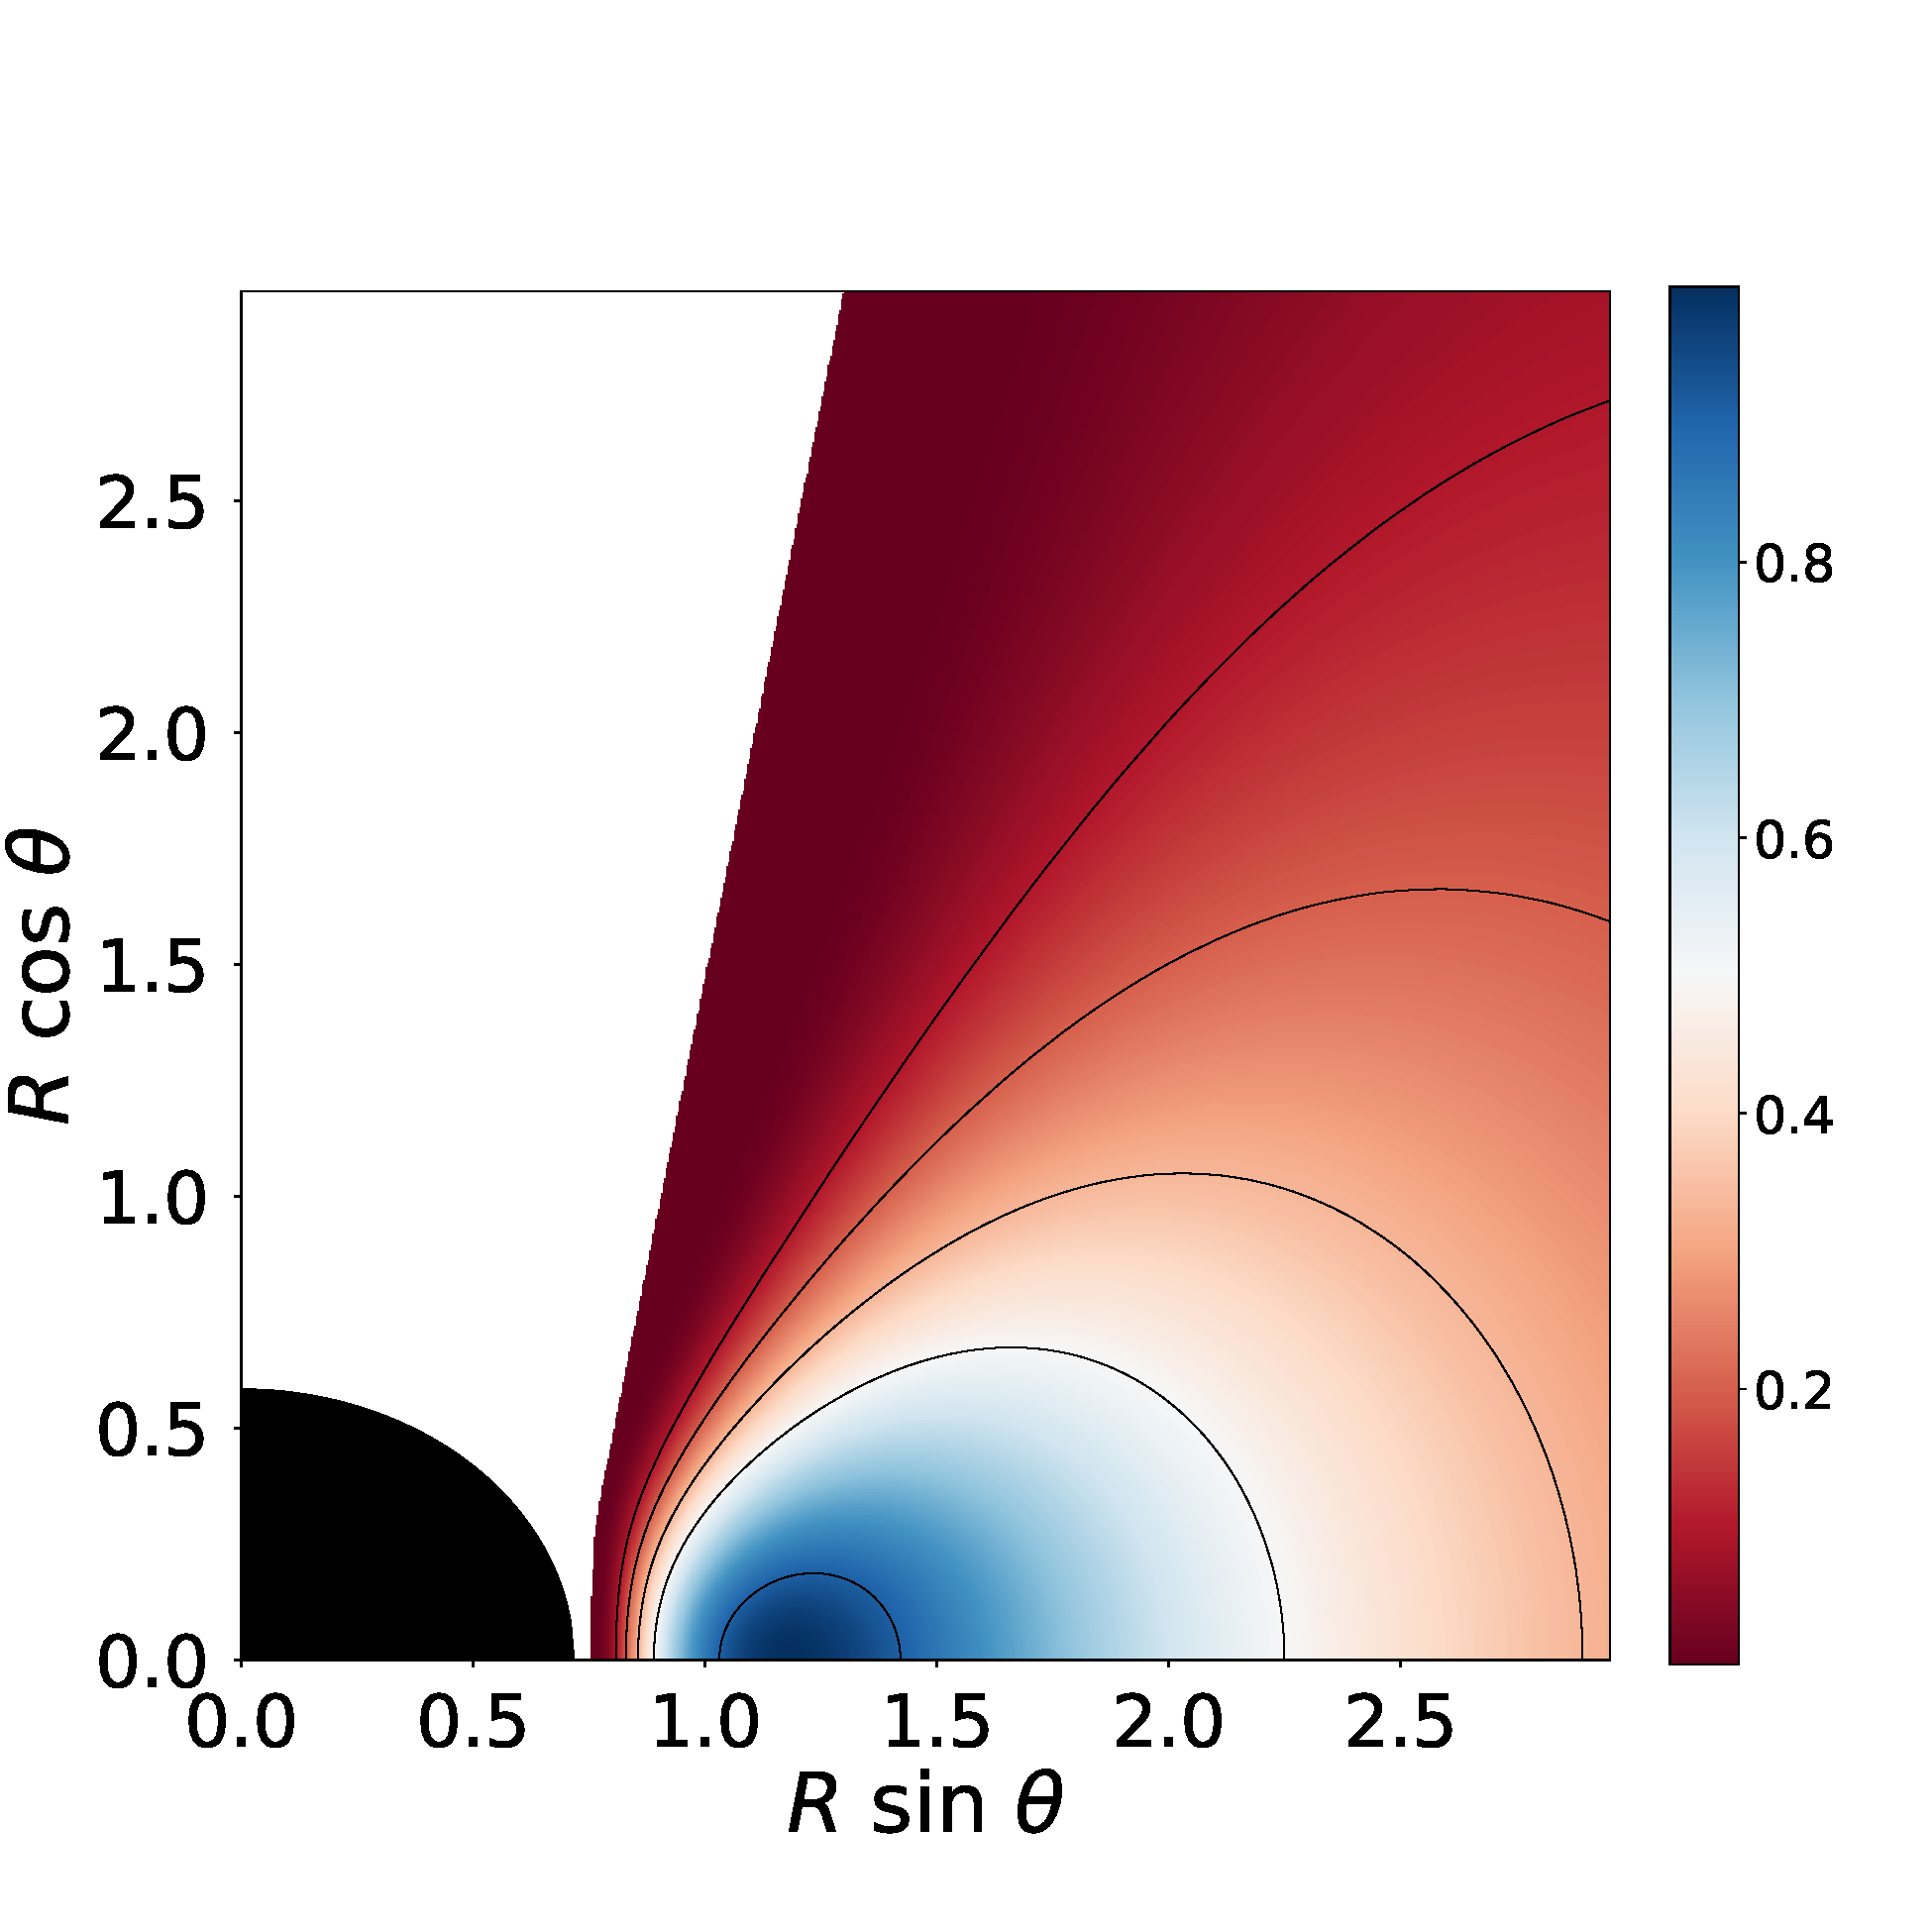
\includegraphics[scale=0.14]{figures/fig3_II_10.pdf}
\hspace{-0.3cm}
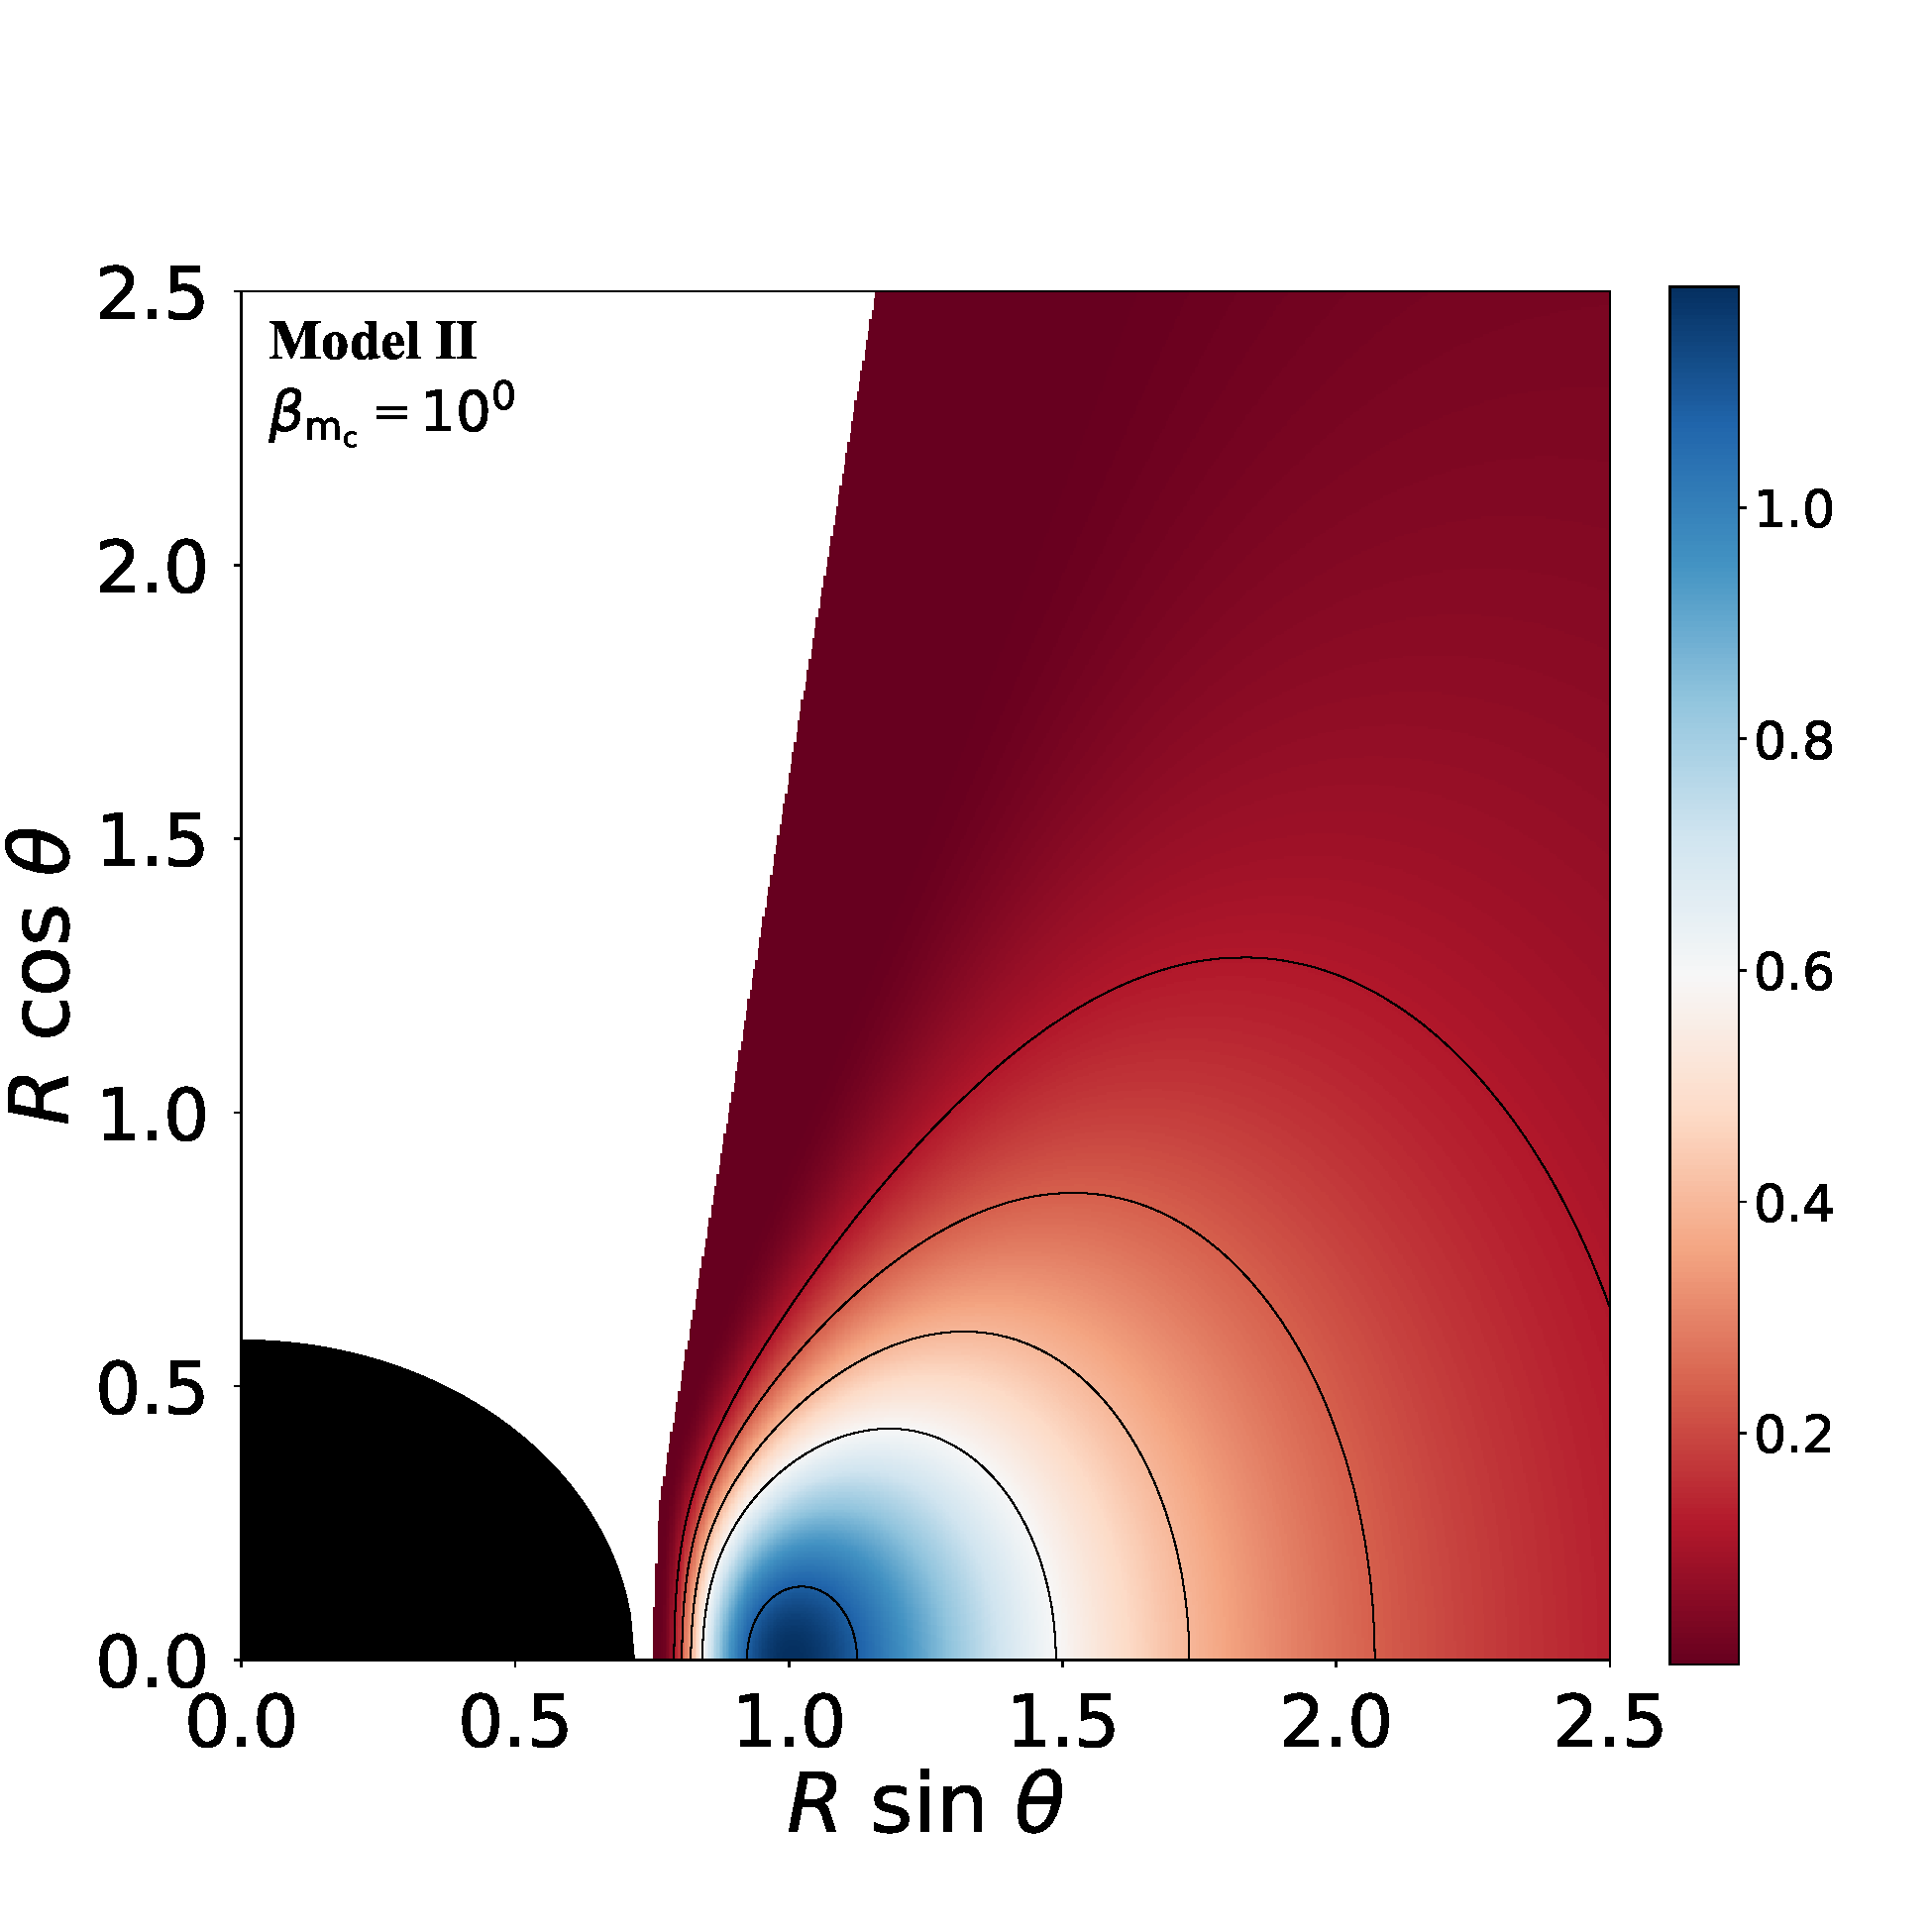
\includegraphics[scale=0.14]{figures/fig3_II_1.pdf}
\hspace{-0.2cm}
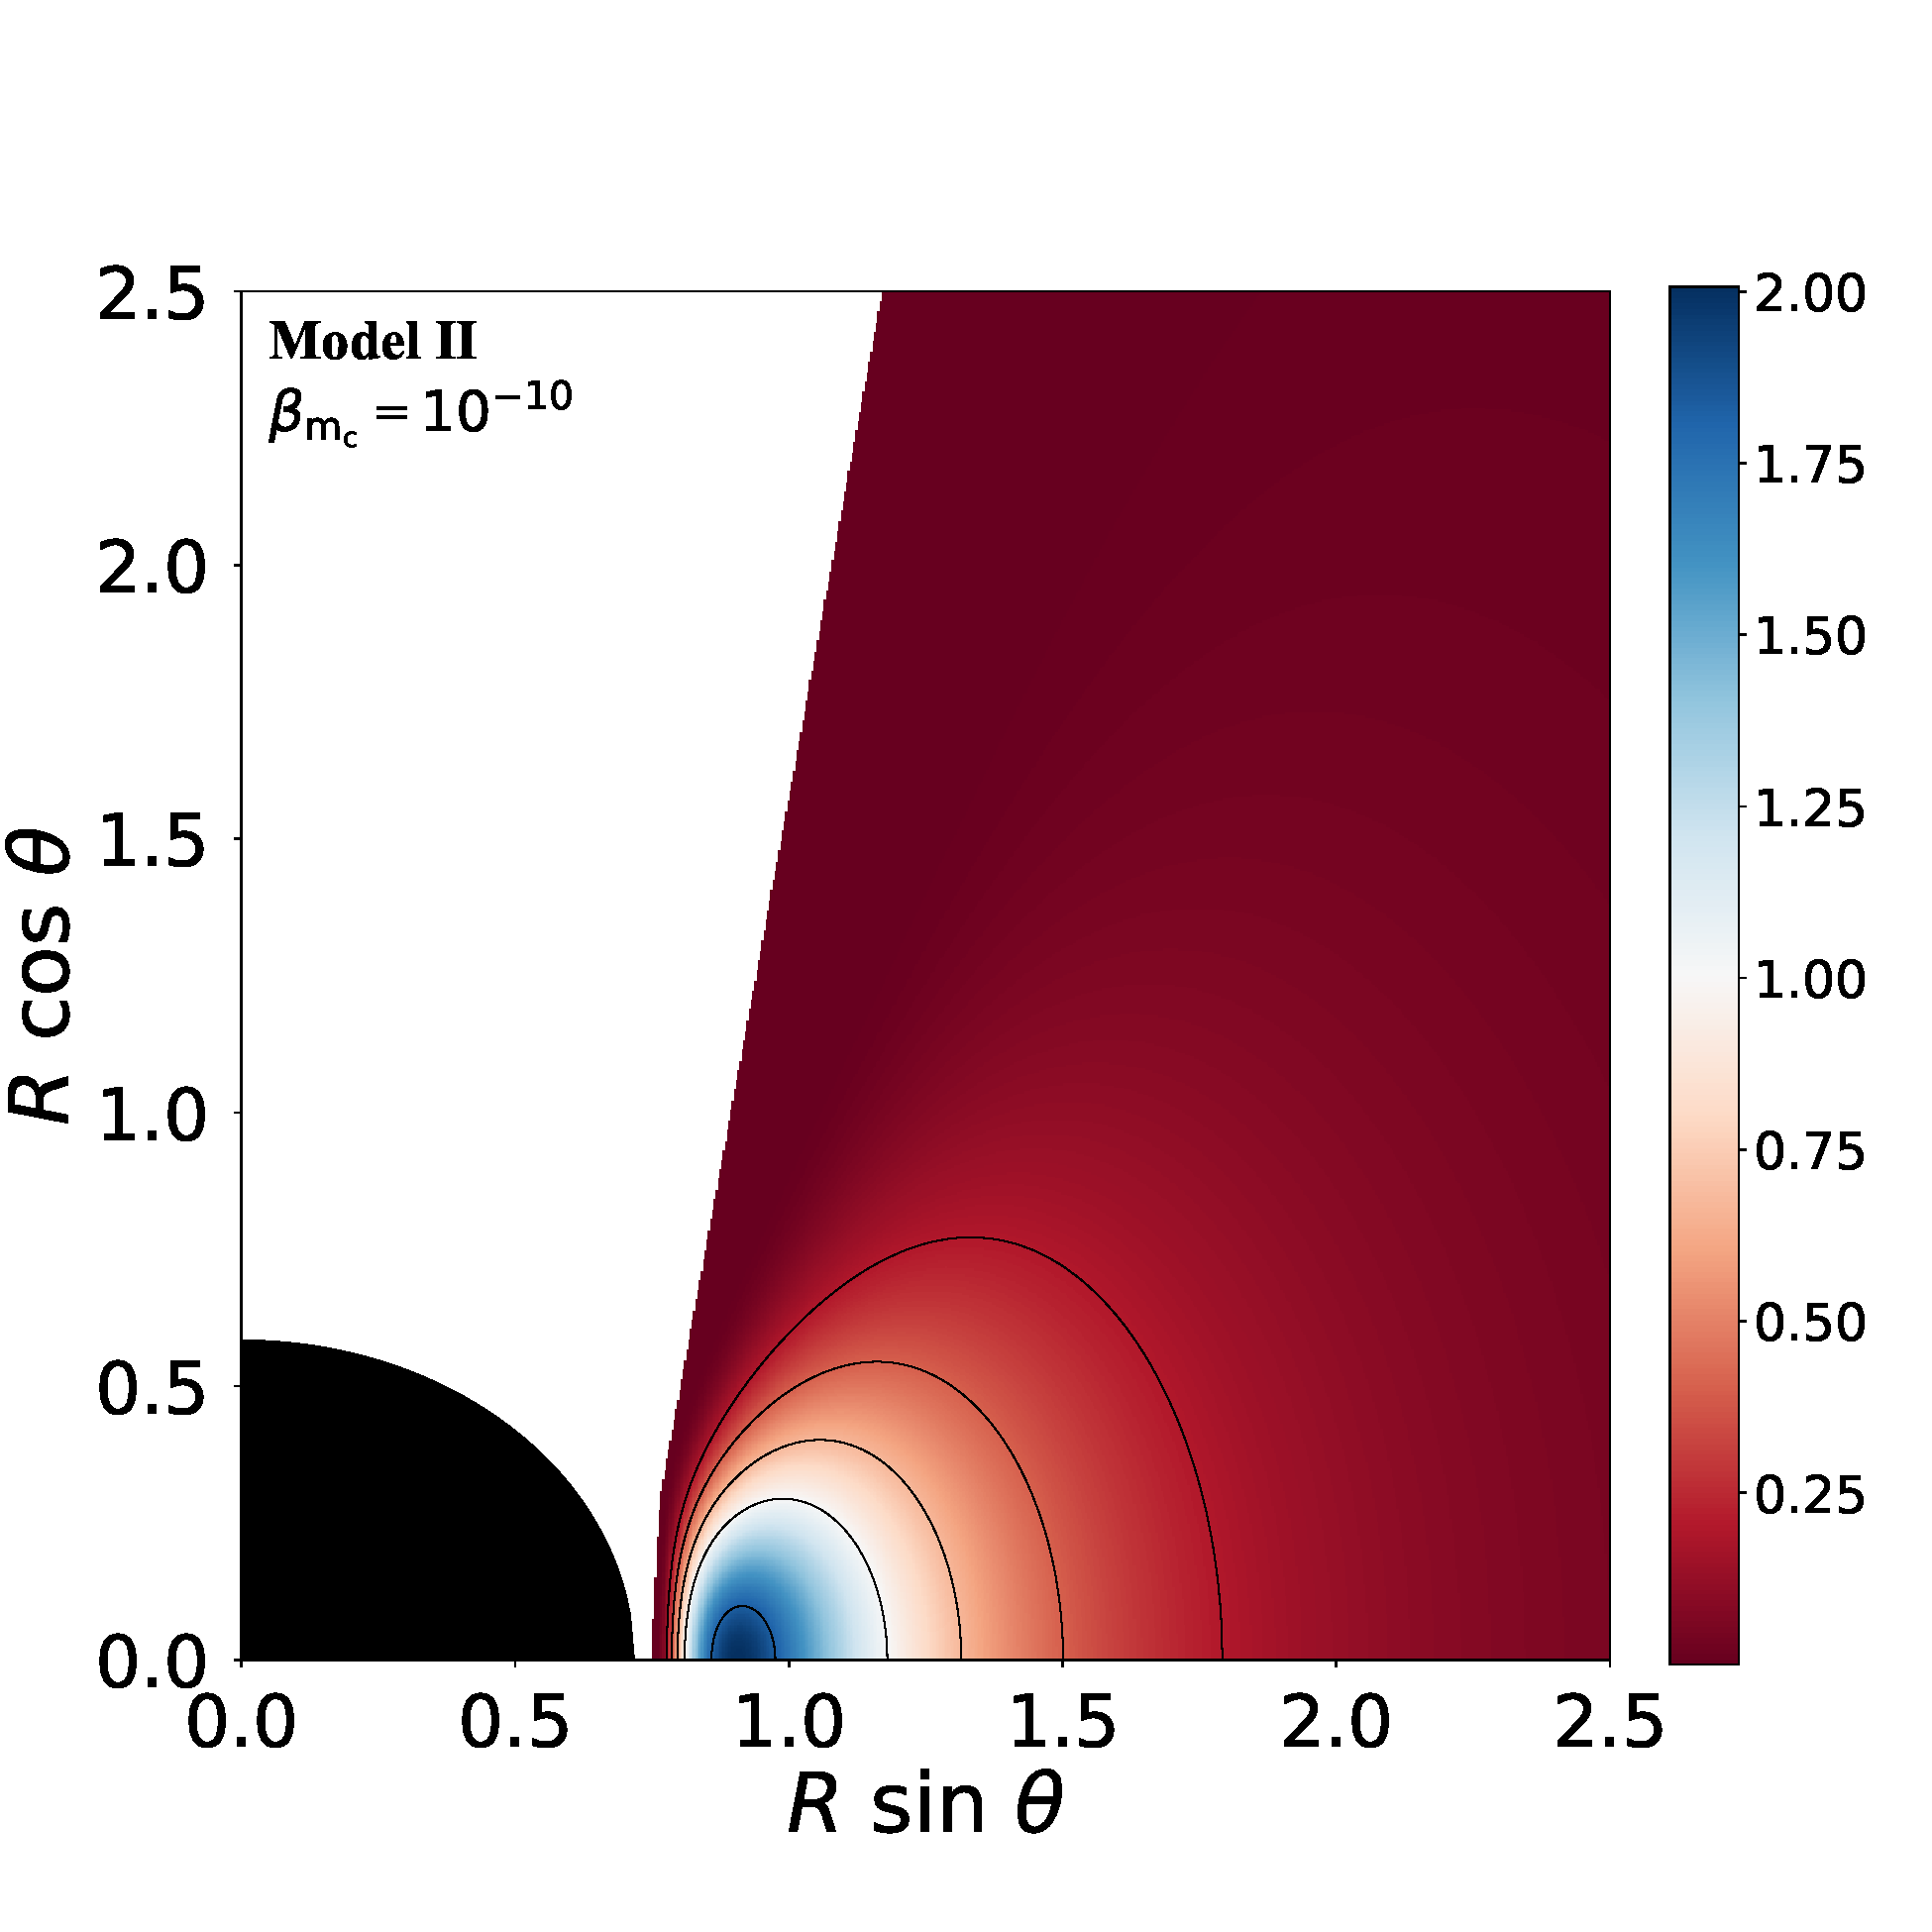
\includegraphics[scale=0.14]{figures/fig3_II__10.pdf}
\\
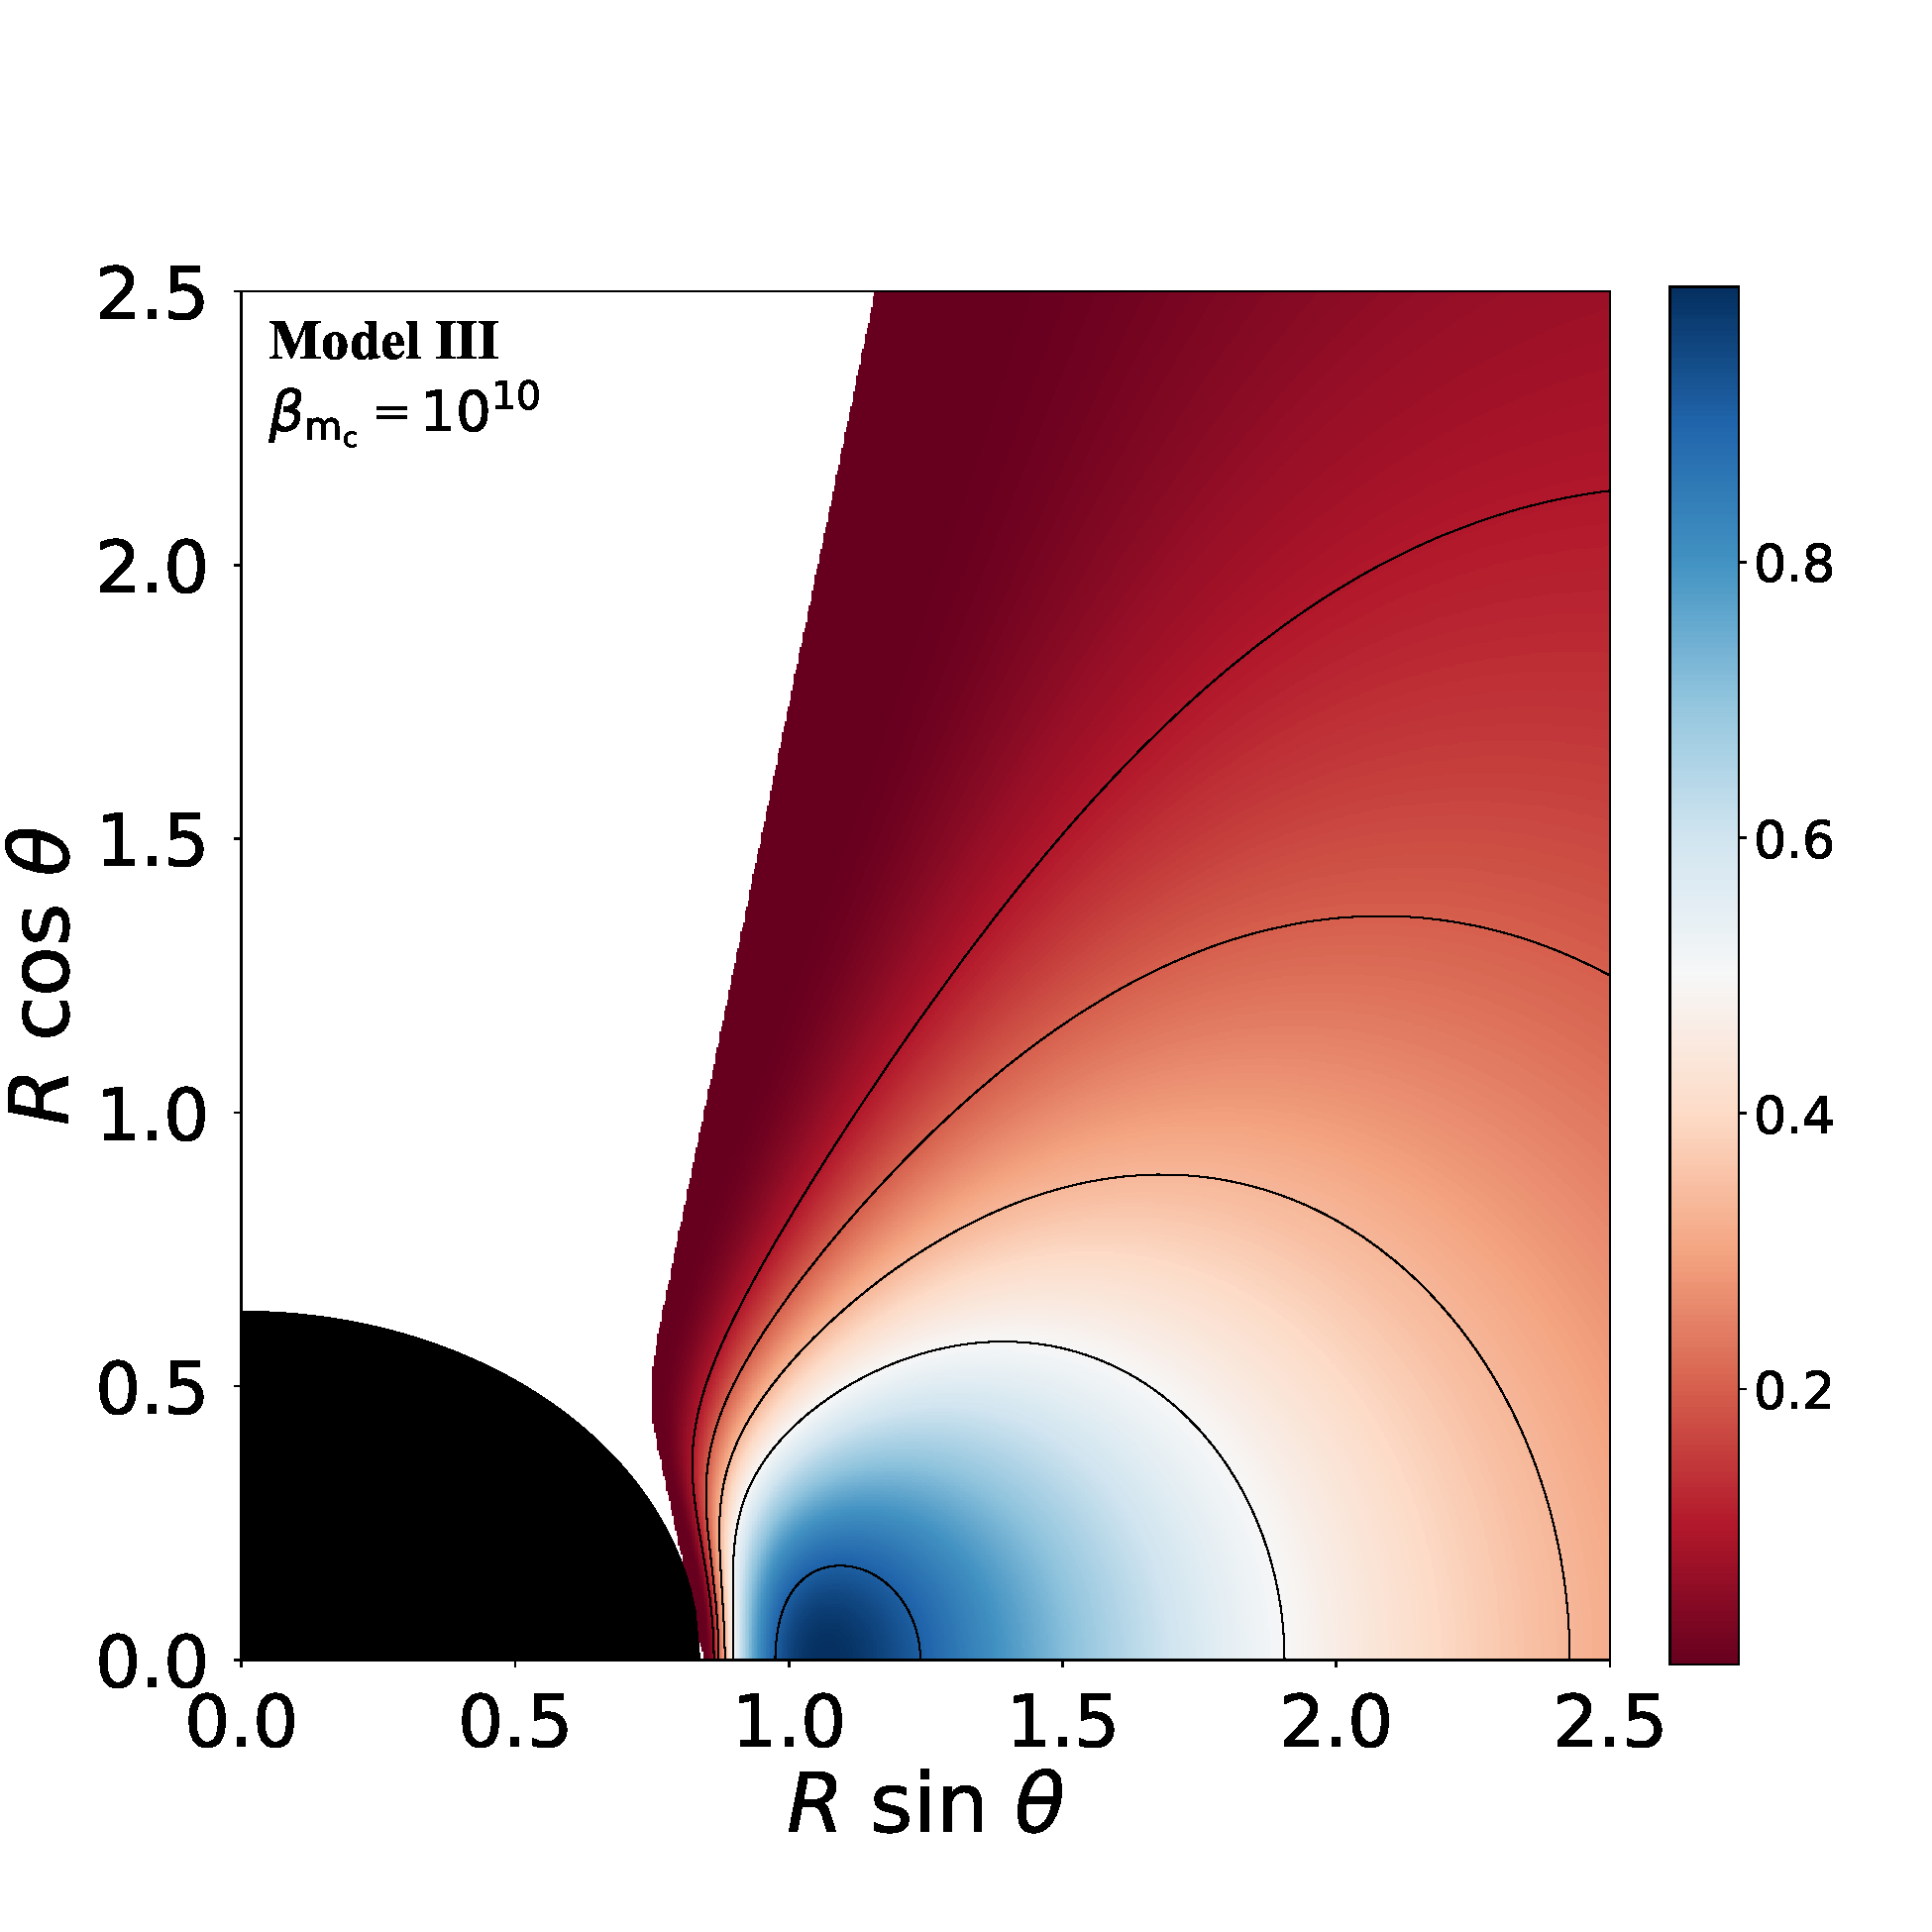
\includegraphics[scale=0.14]{figures/fig3_III_10.pdf}
\hspace{-0.3cm}
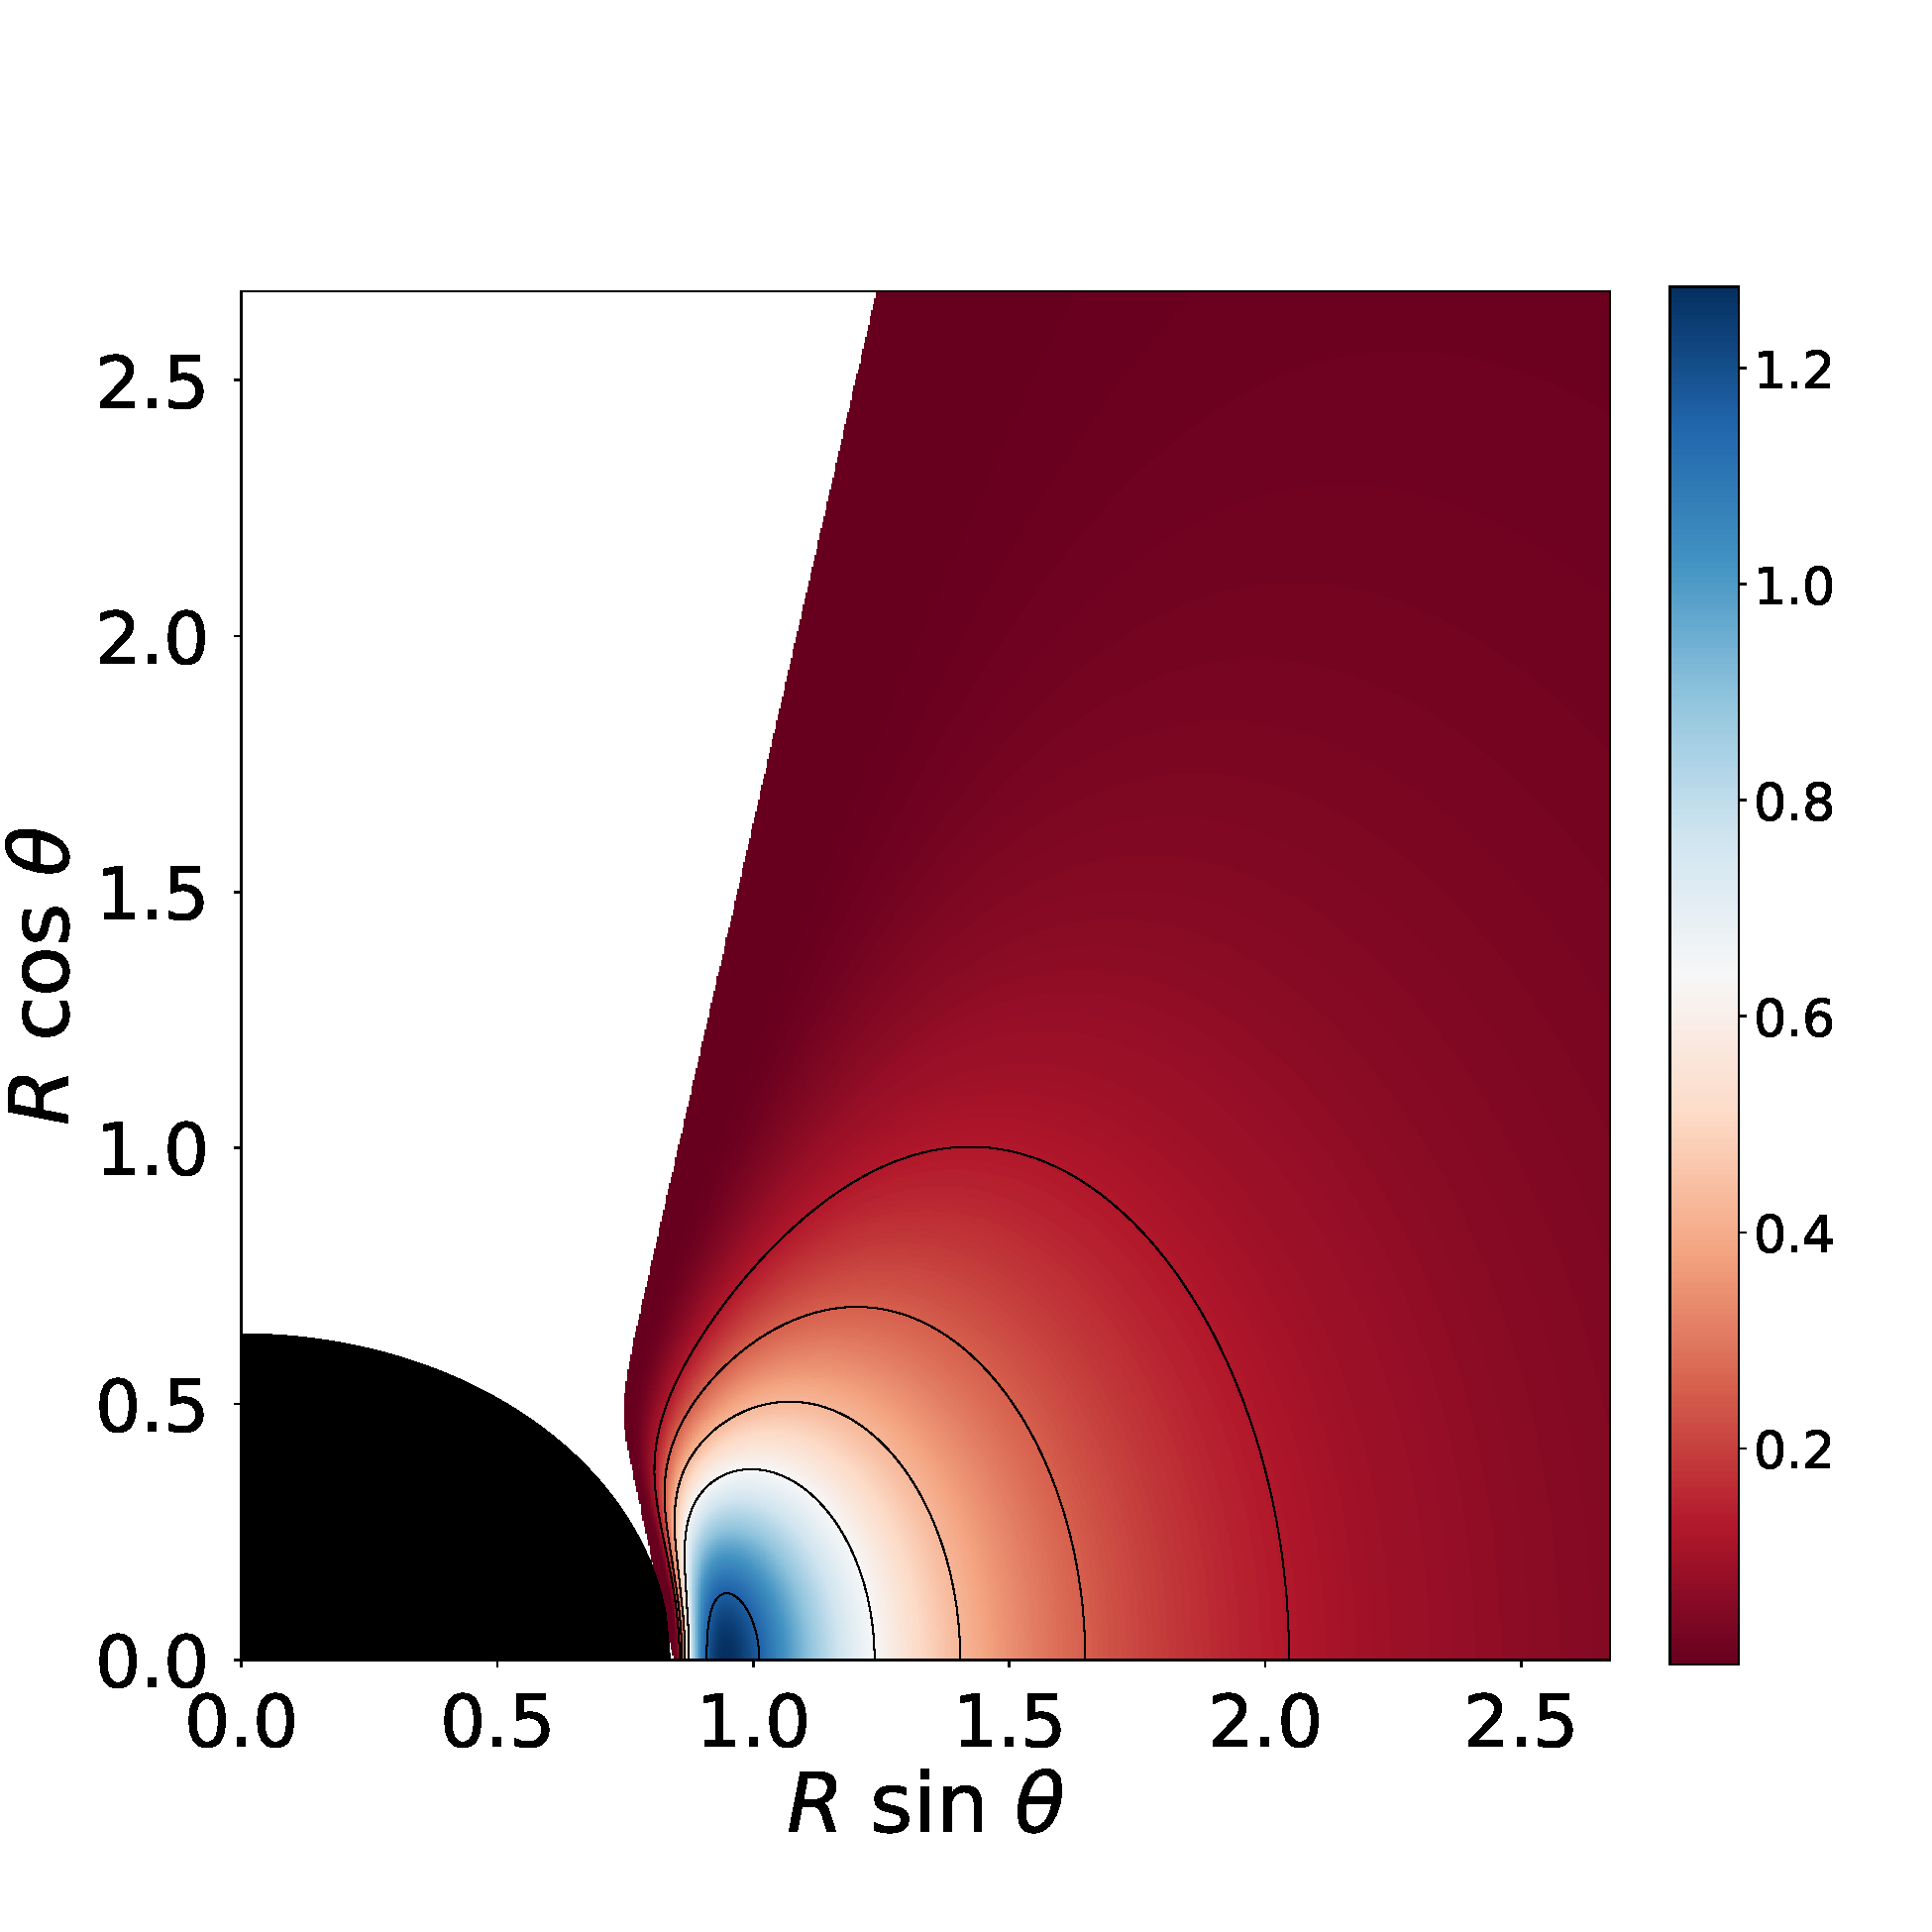
\includegraphics[scale=0.14]{figures/fig3_III_1.pdf}
\hspace{-0.2cm}
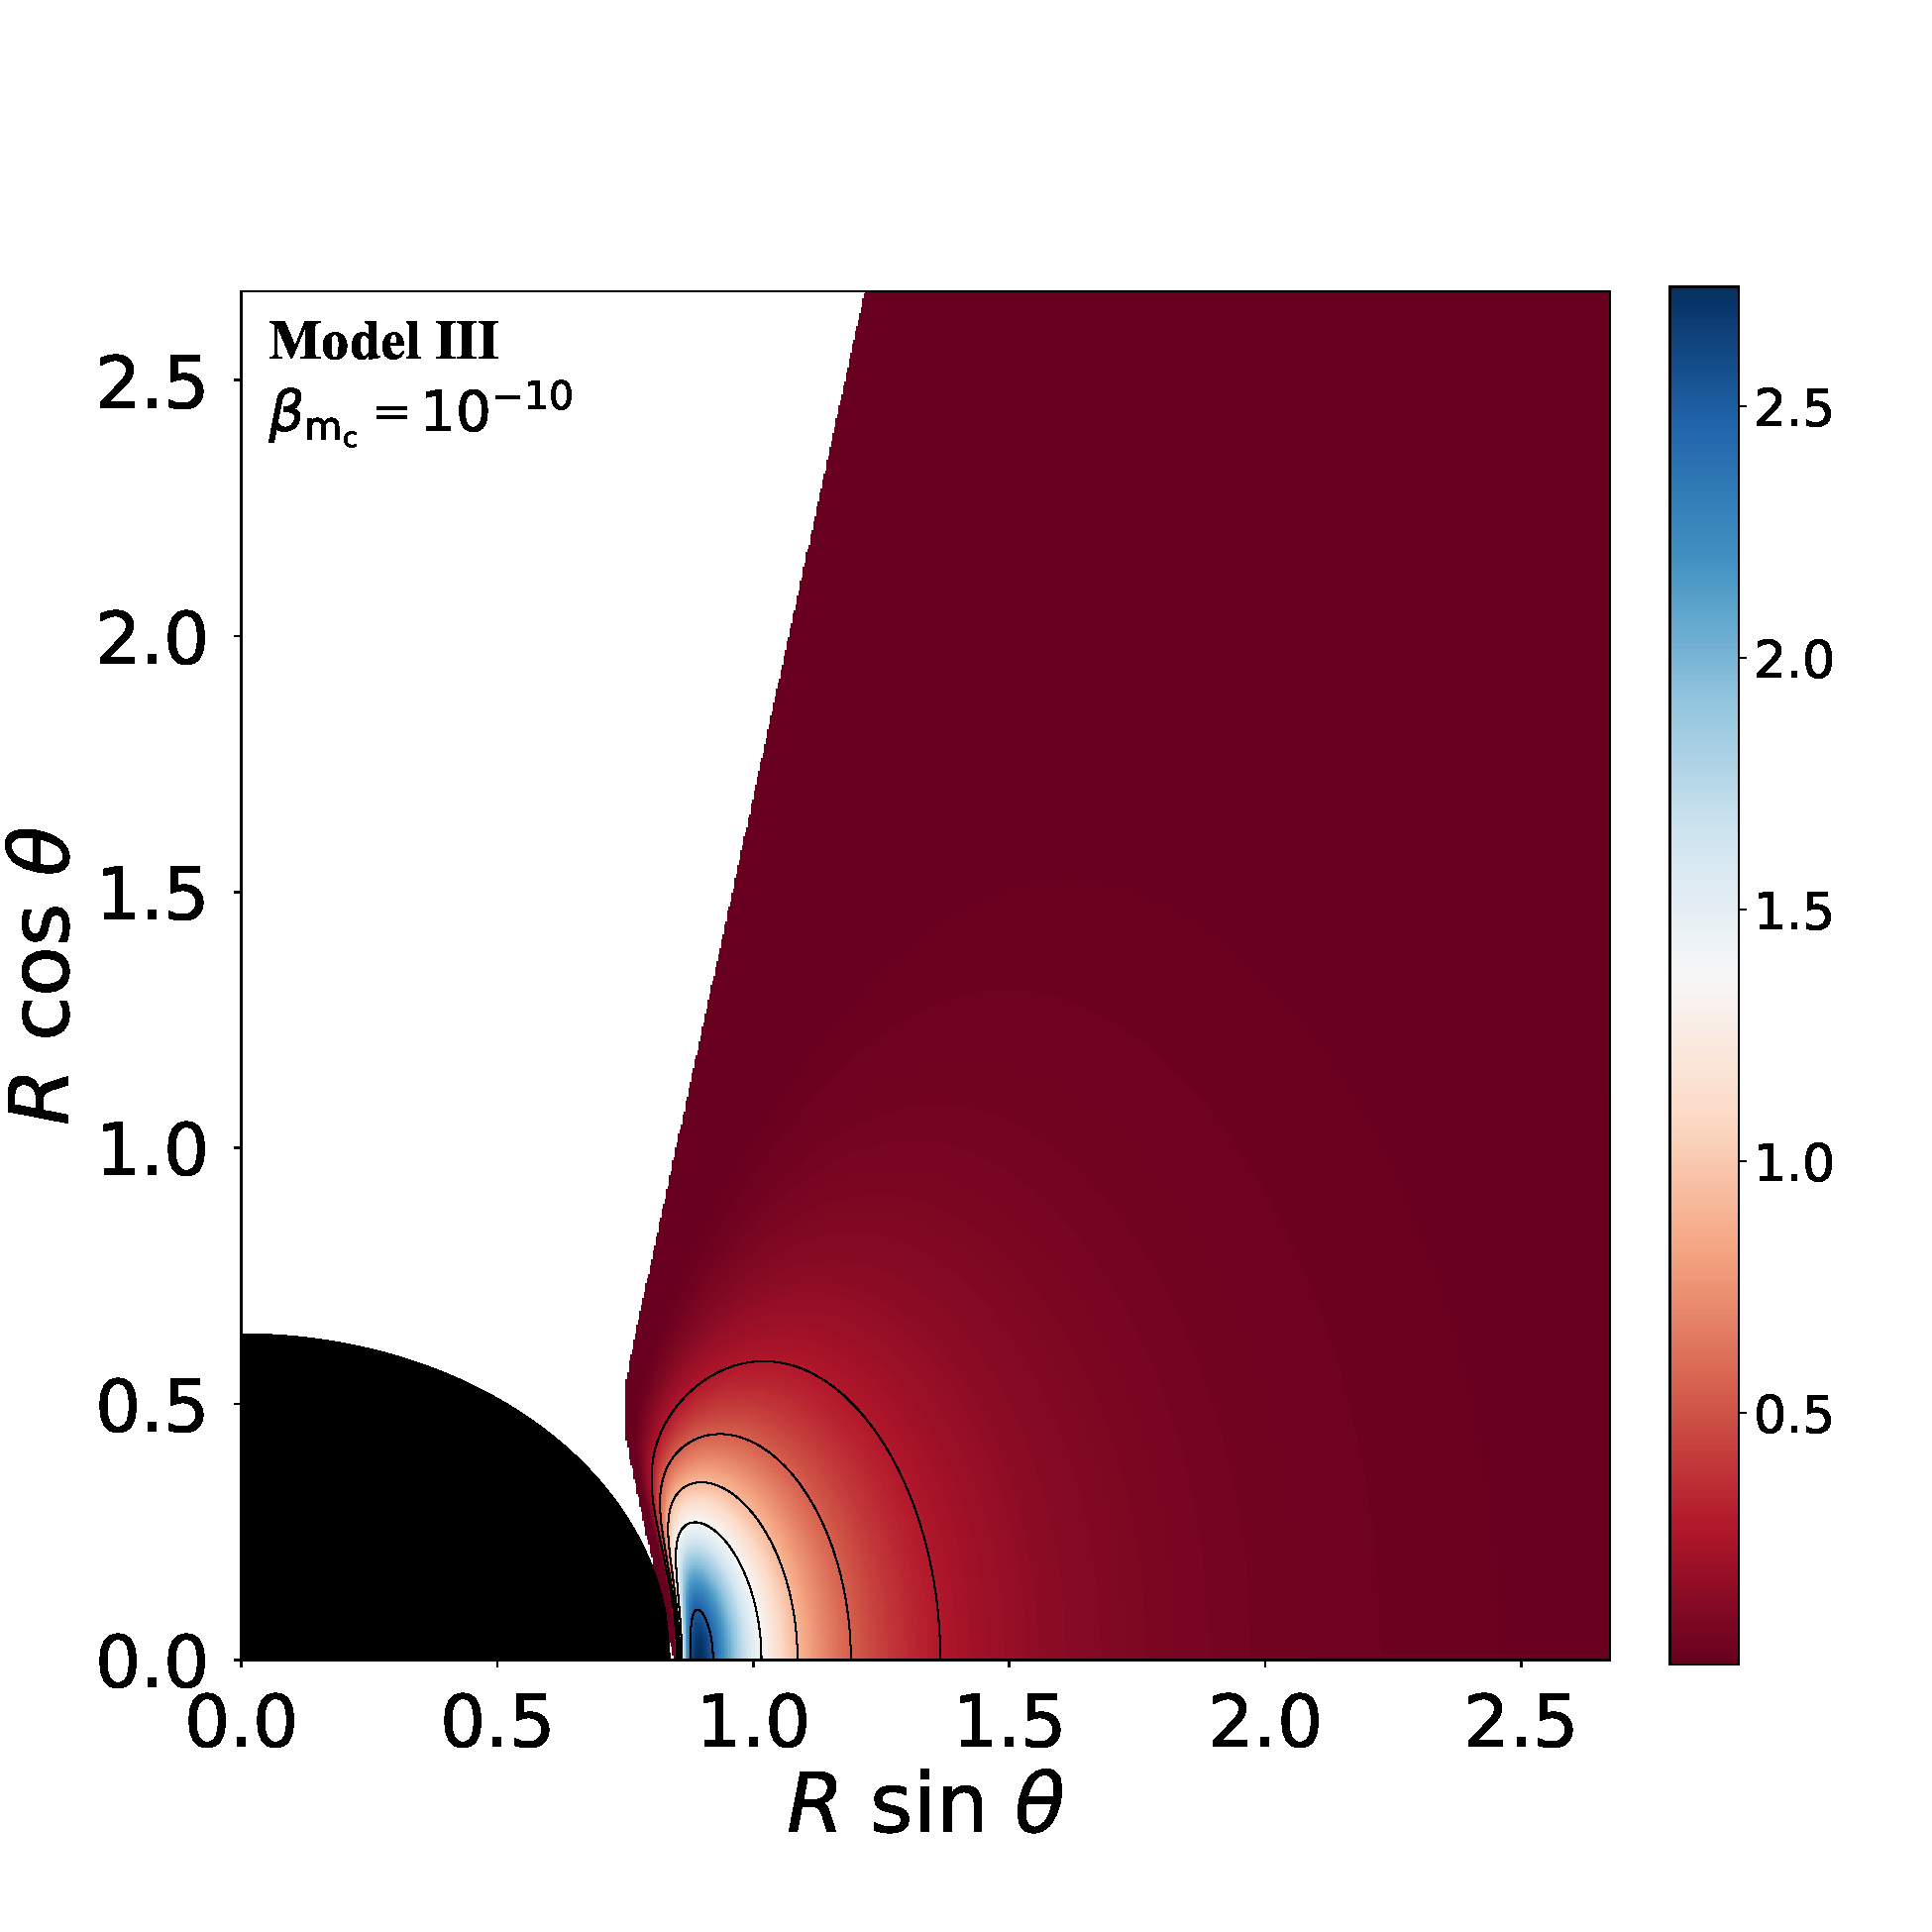
\includegraphics[scale=0.14]{figures/fig3_III__10.pdf}
\\
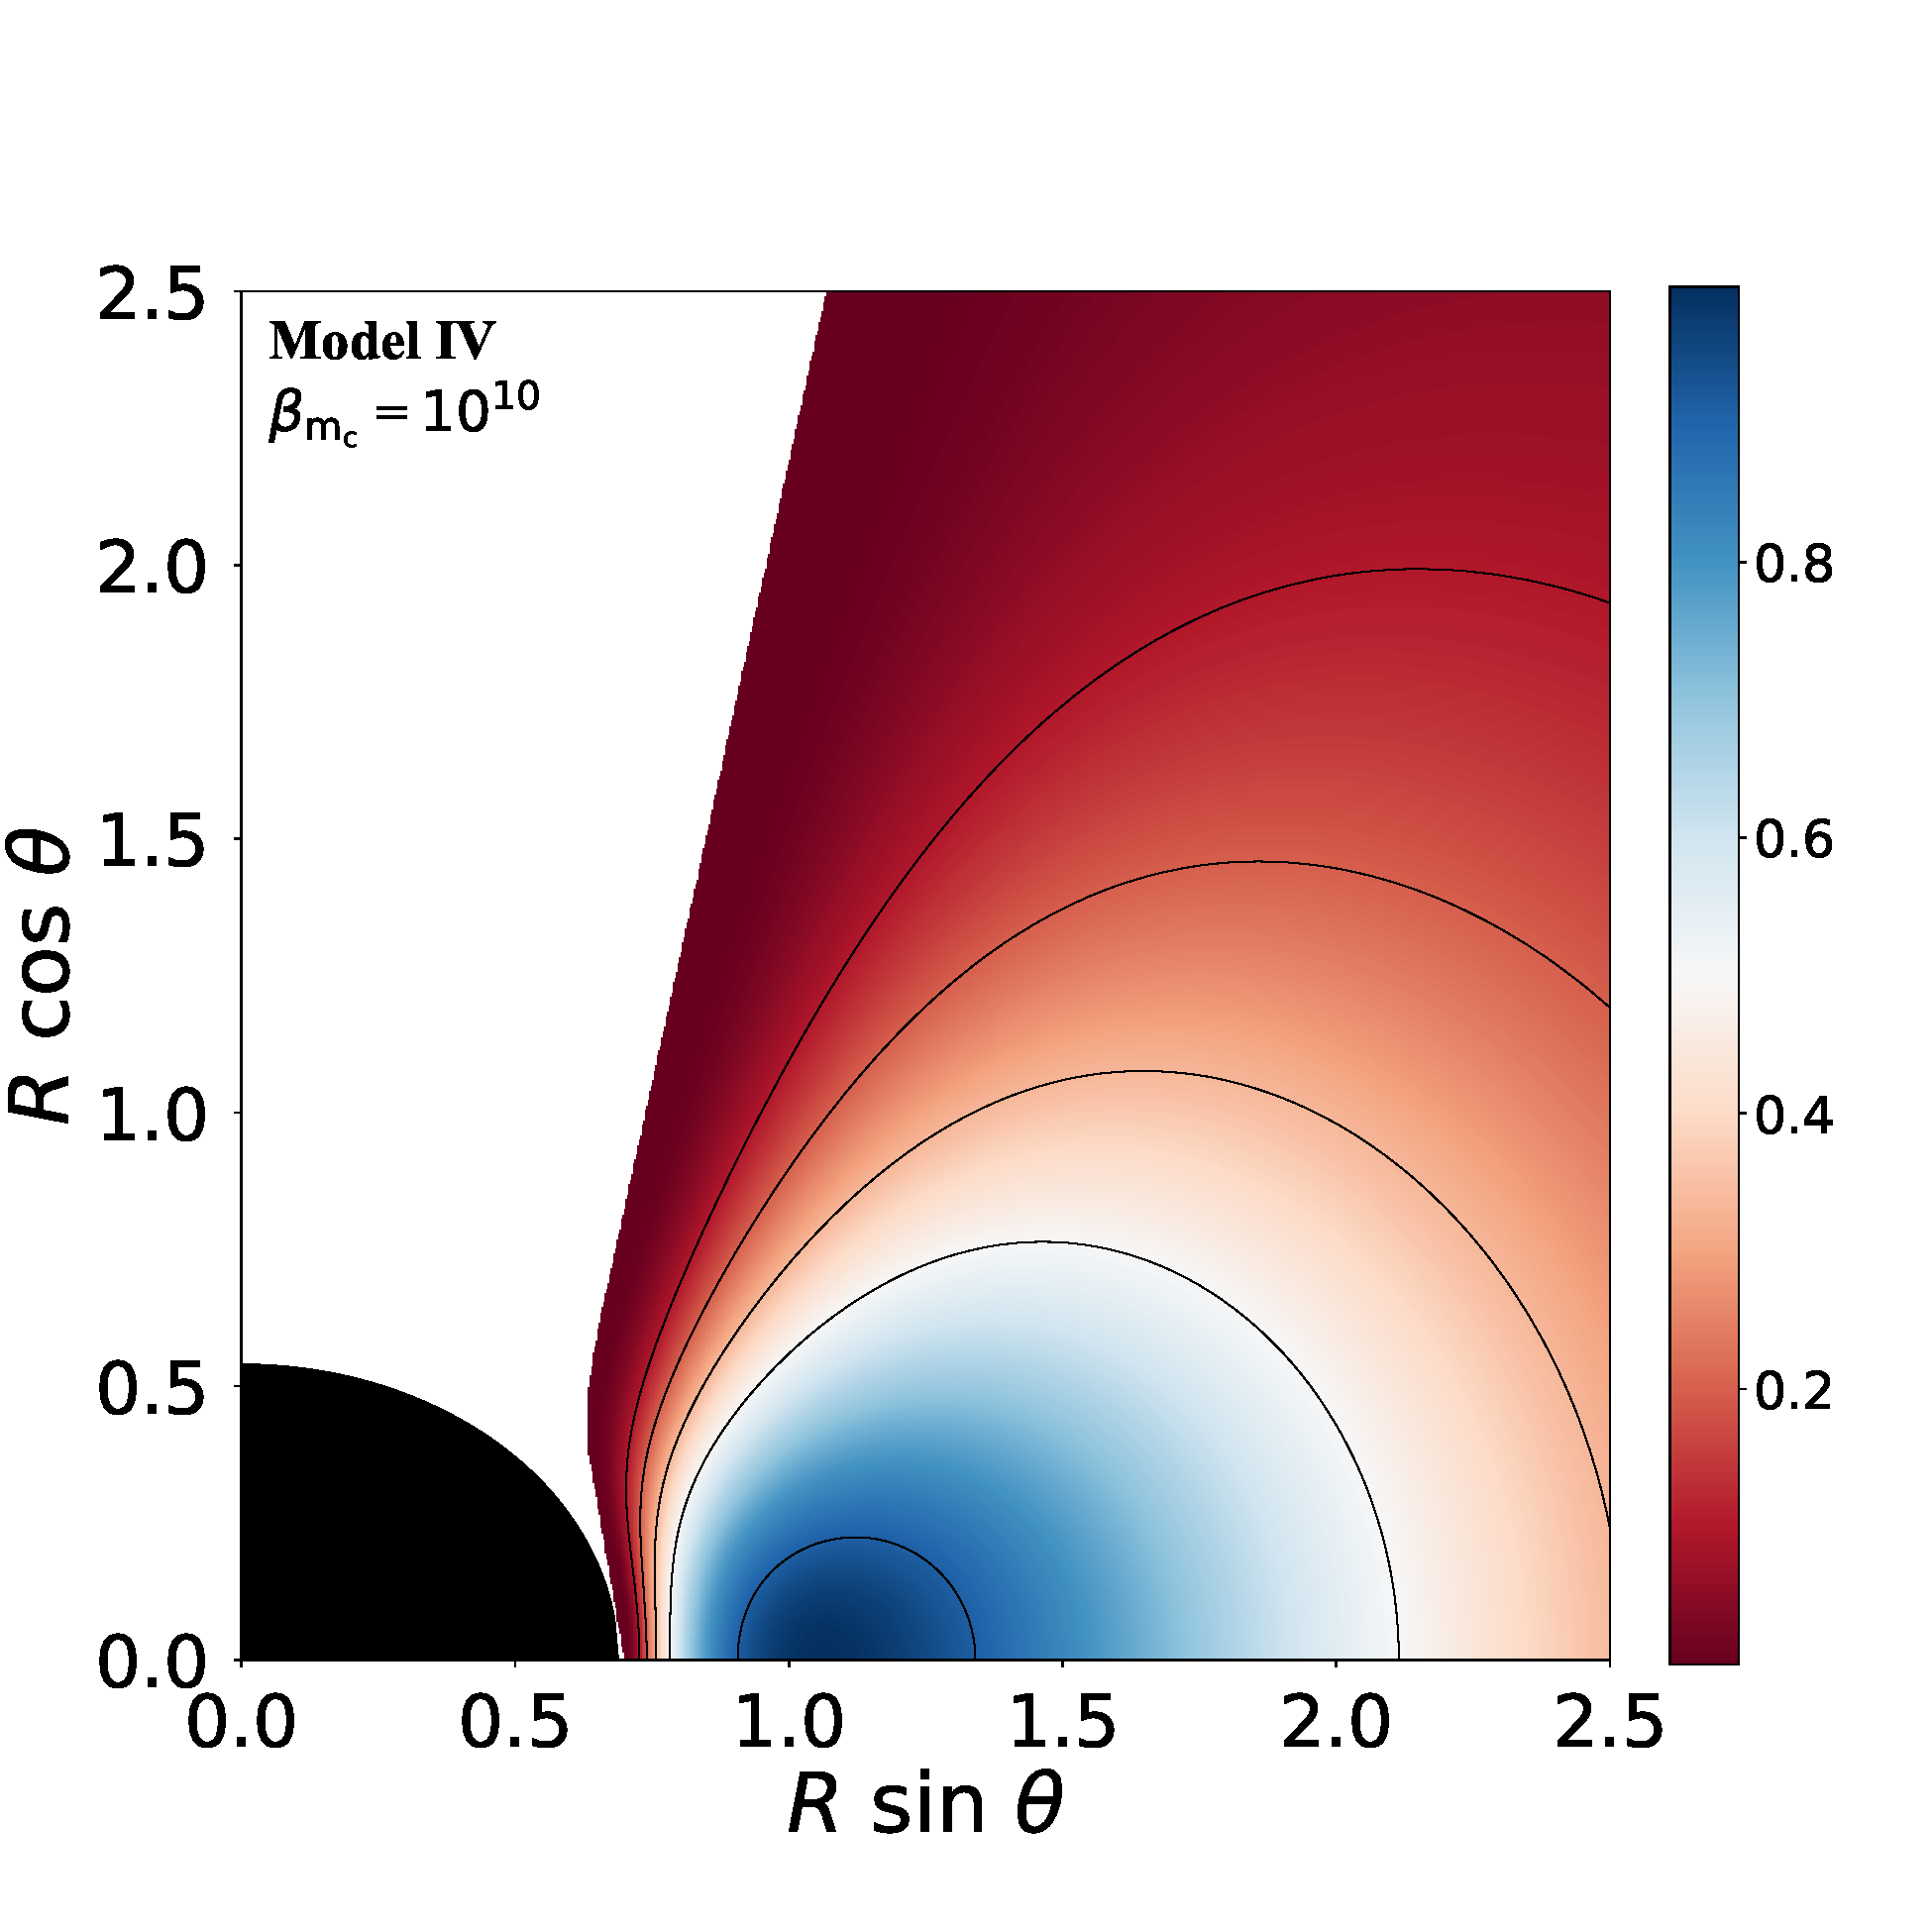
\includegraphics[scale=0.14]{figures/fig3_IV_10.pdf}
\hspace{-0.3cm}
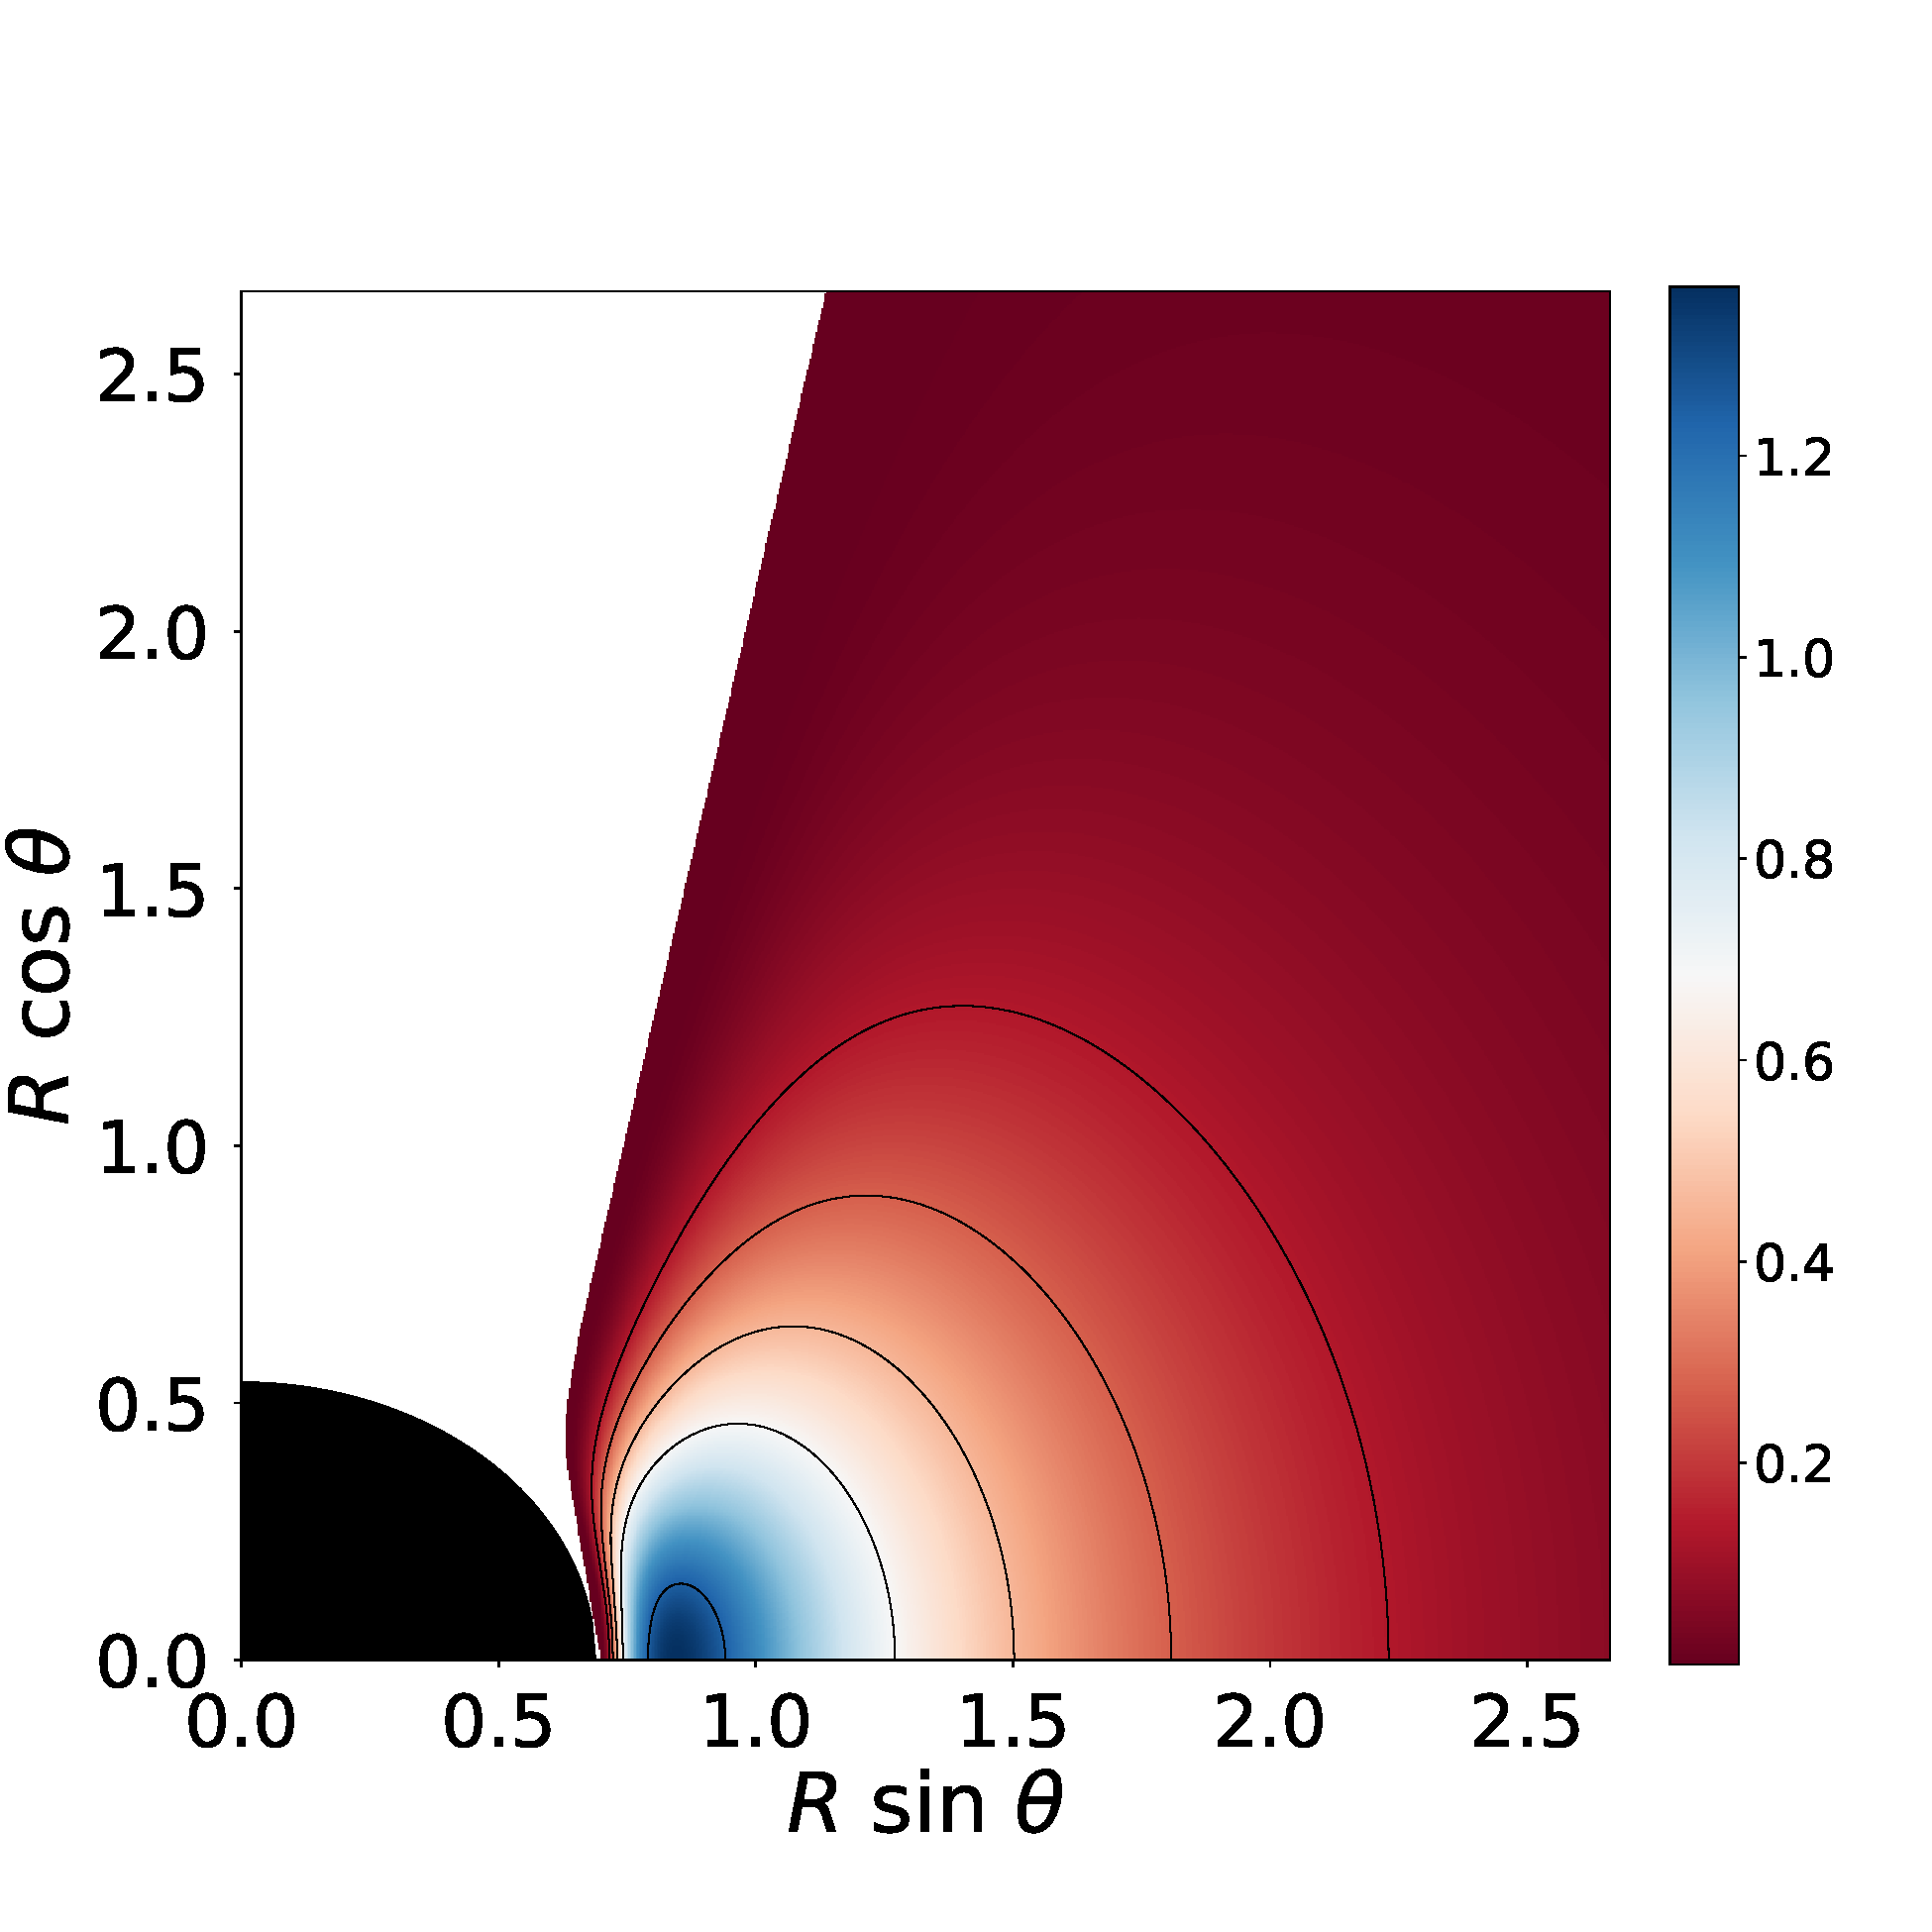
\includegraphics[scale=0.14]{figures/fig3_IV_1.pdf}
\hspace{-0.2cm}
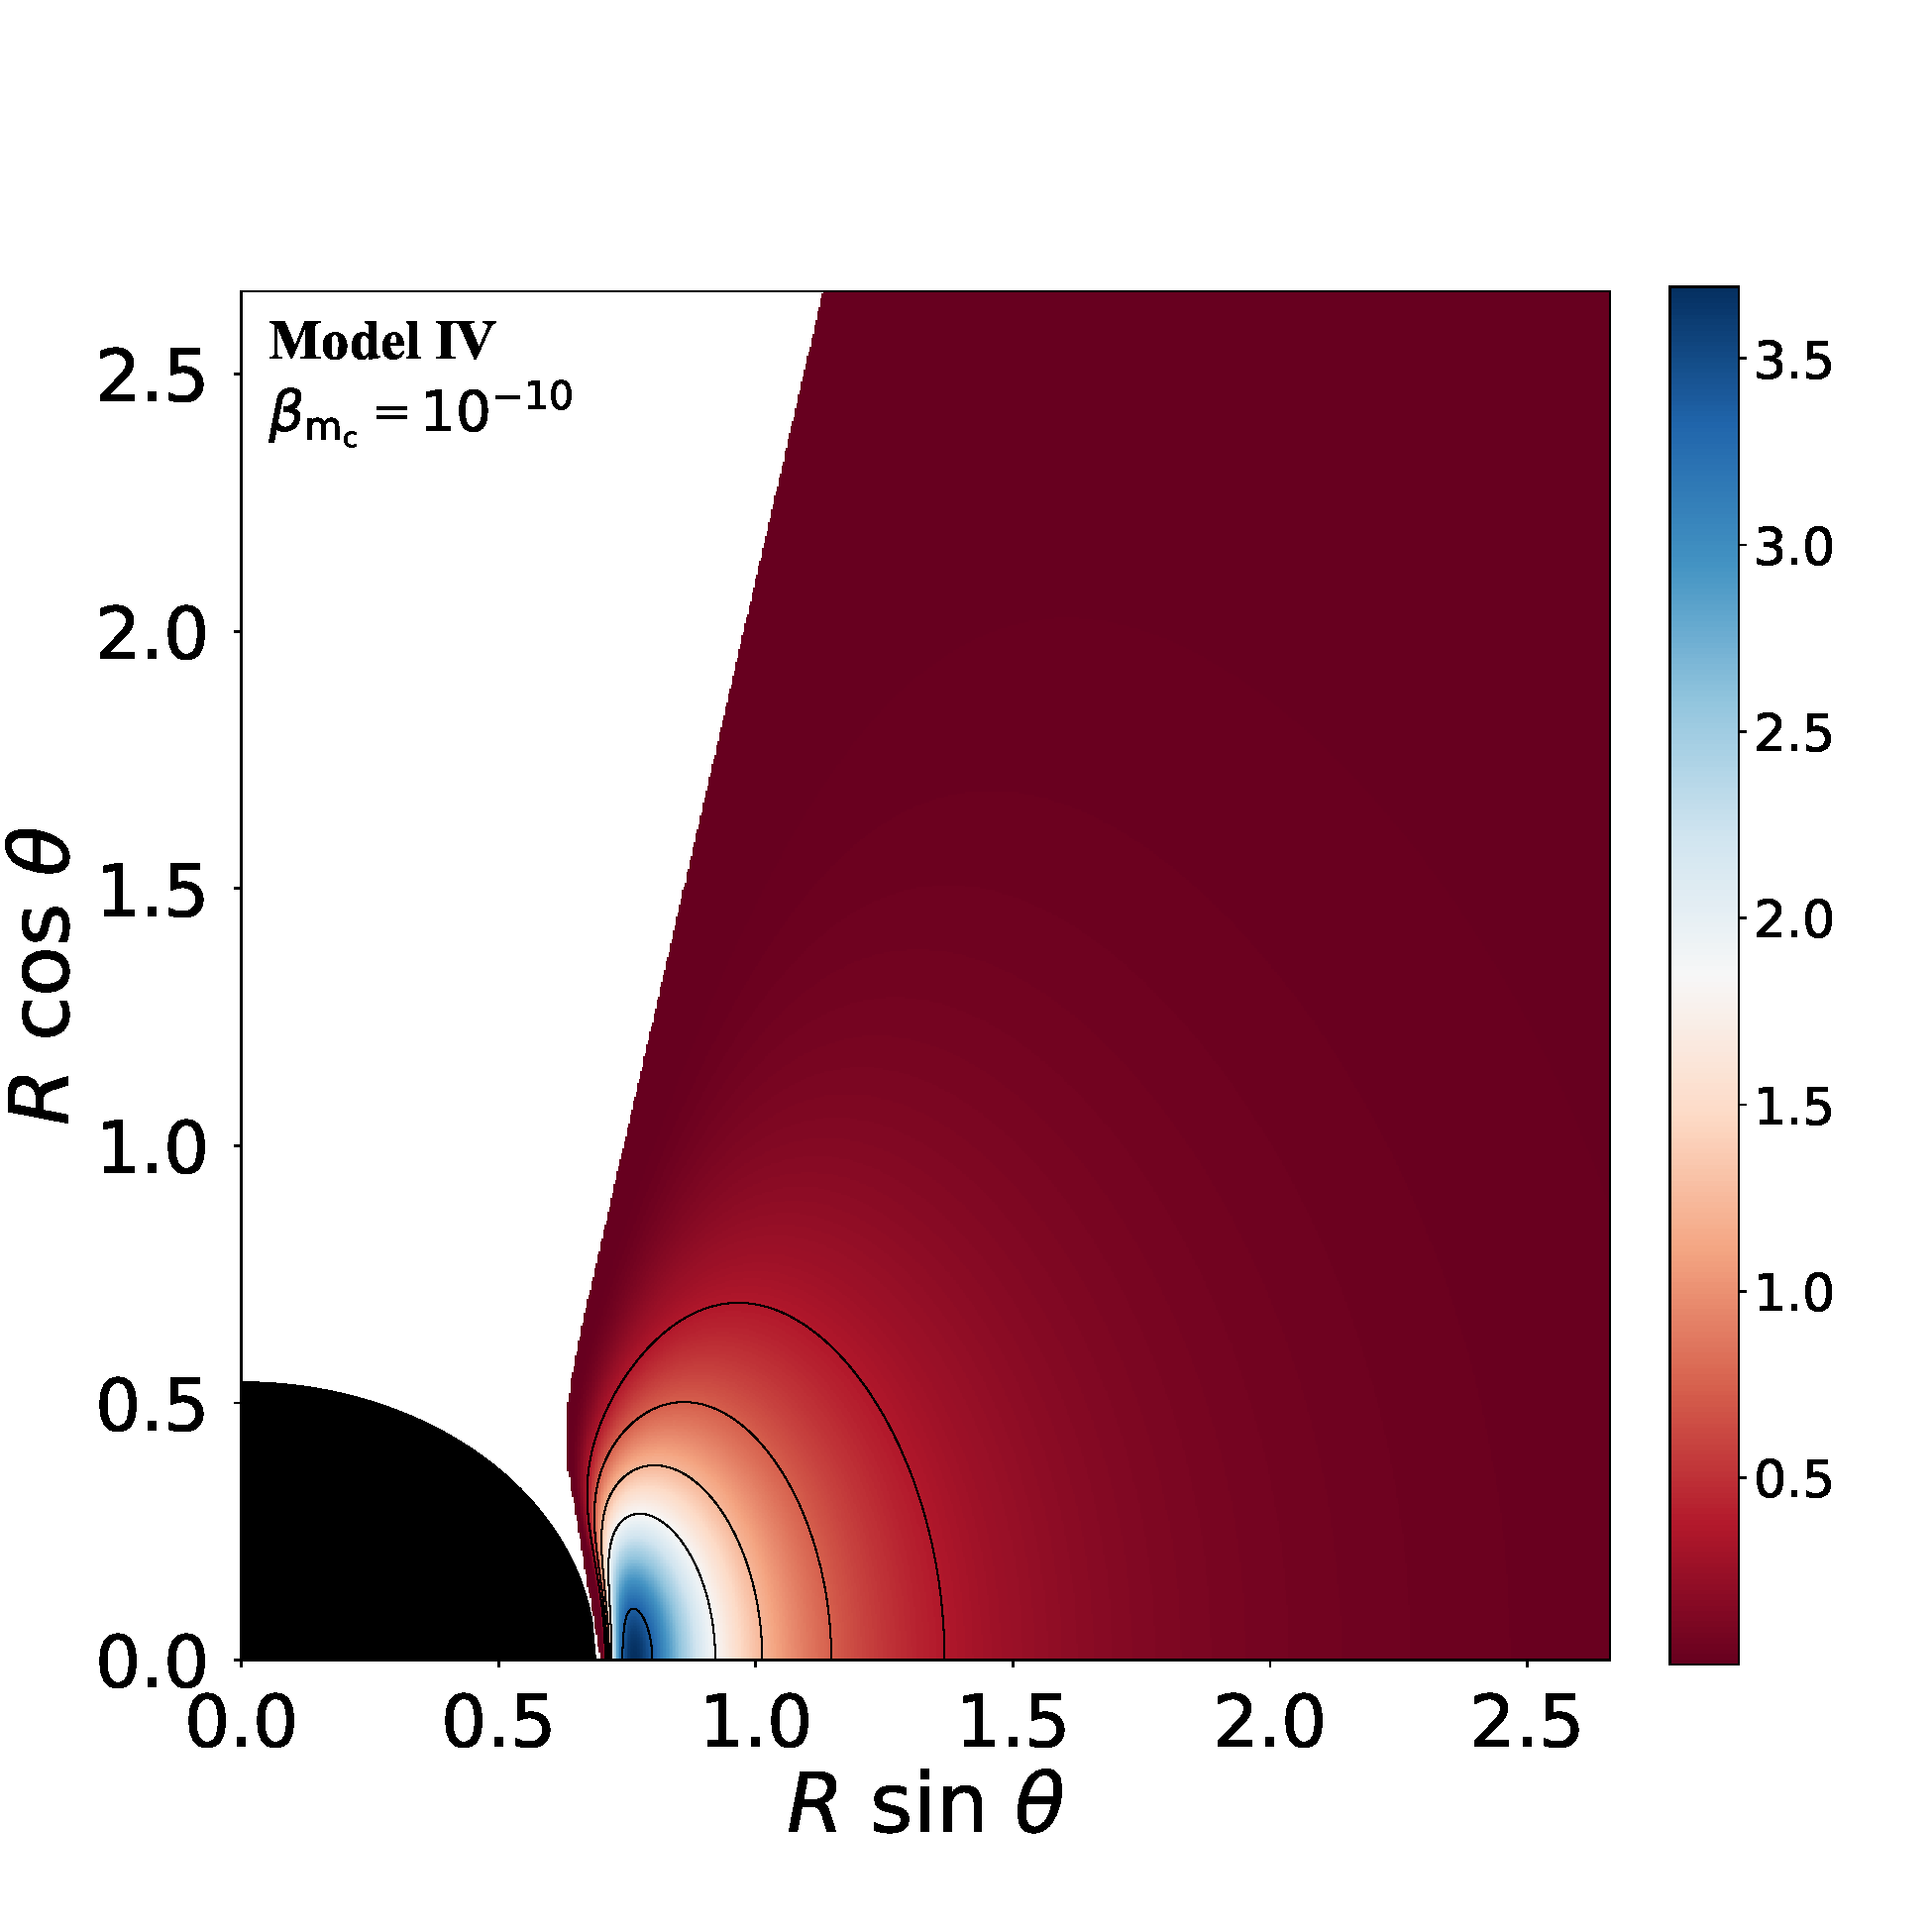
\includegraphics[scale=0.14]{figures/fig3_IV__10.pdf}
\hspace{-0.2cm}
\caption{Same as Fig.~\ref{models_I} but using the perimetral radial coordinate $R$.}
\label{models_peri_I}
\end{figure*}

\begin{figure*}
\centering
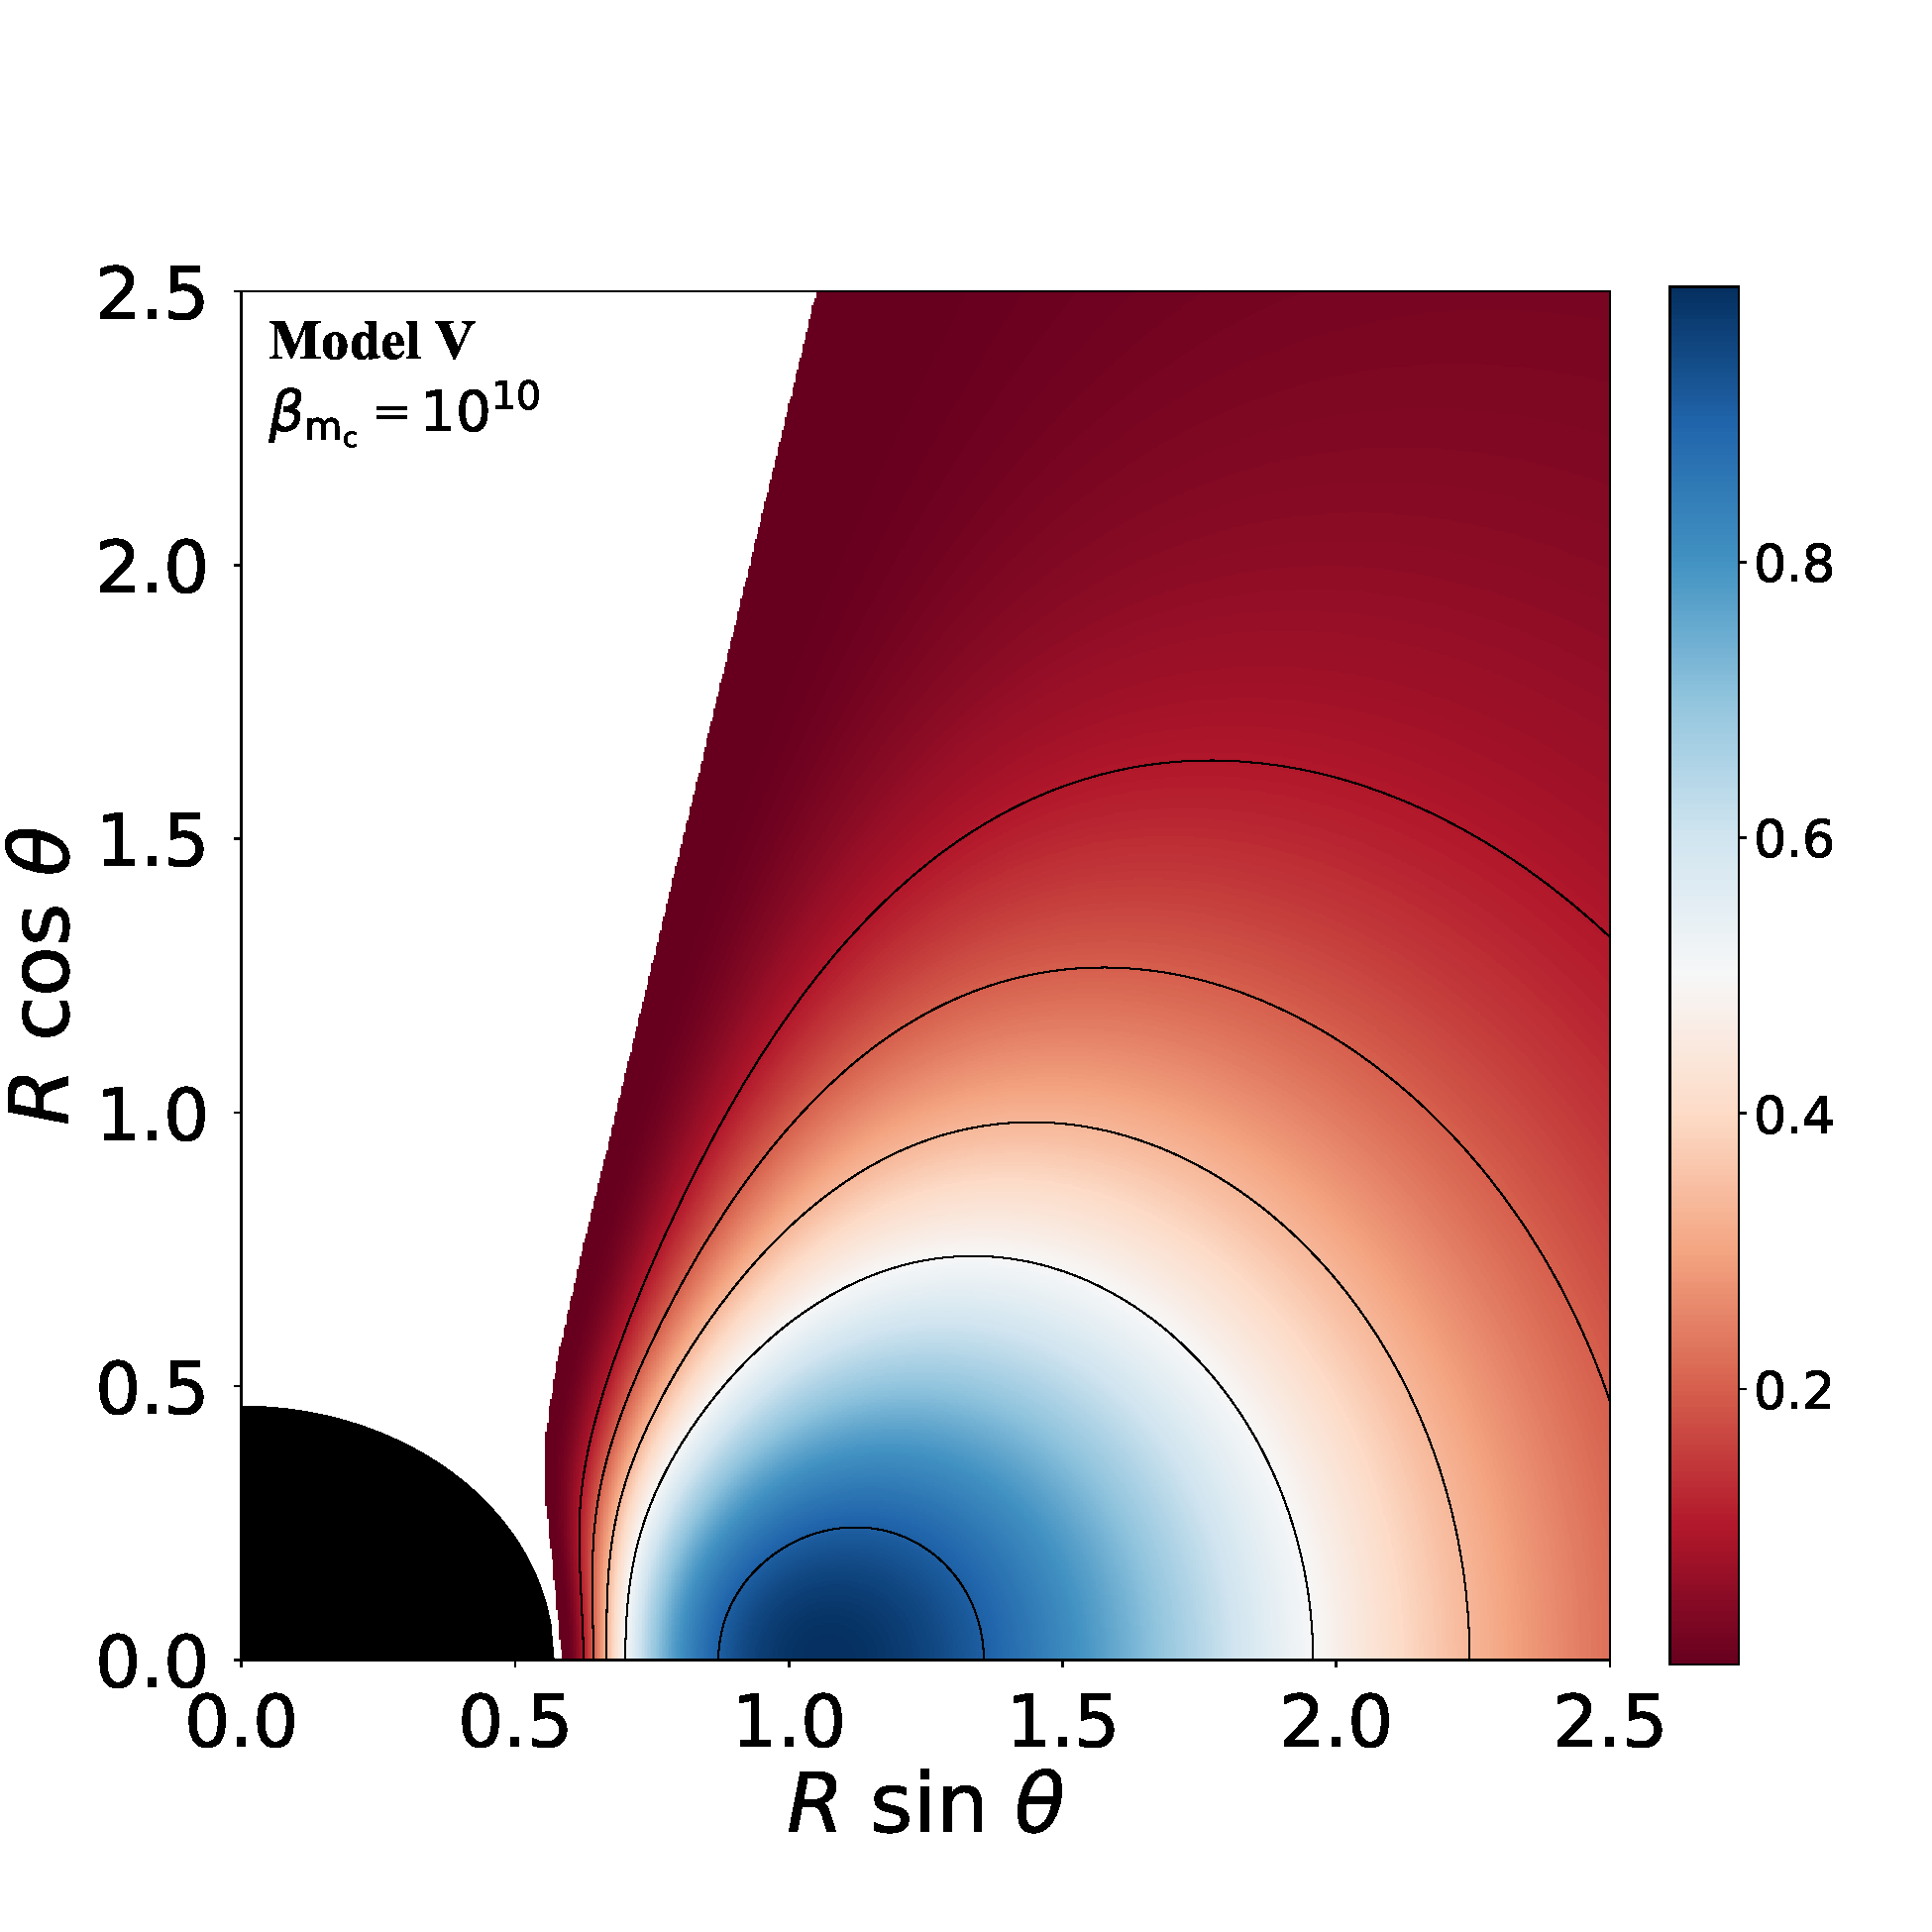
\includegraphics[scale=0.14]{figures/fig4_V_10.pdf}
\hspace{-0.3cm}
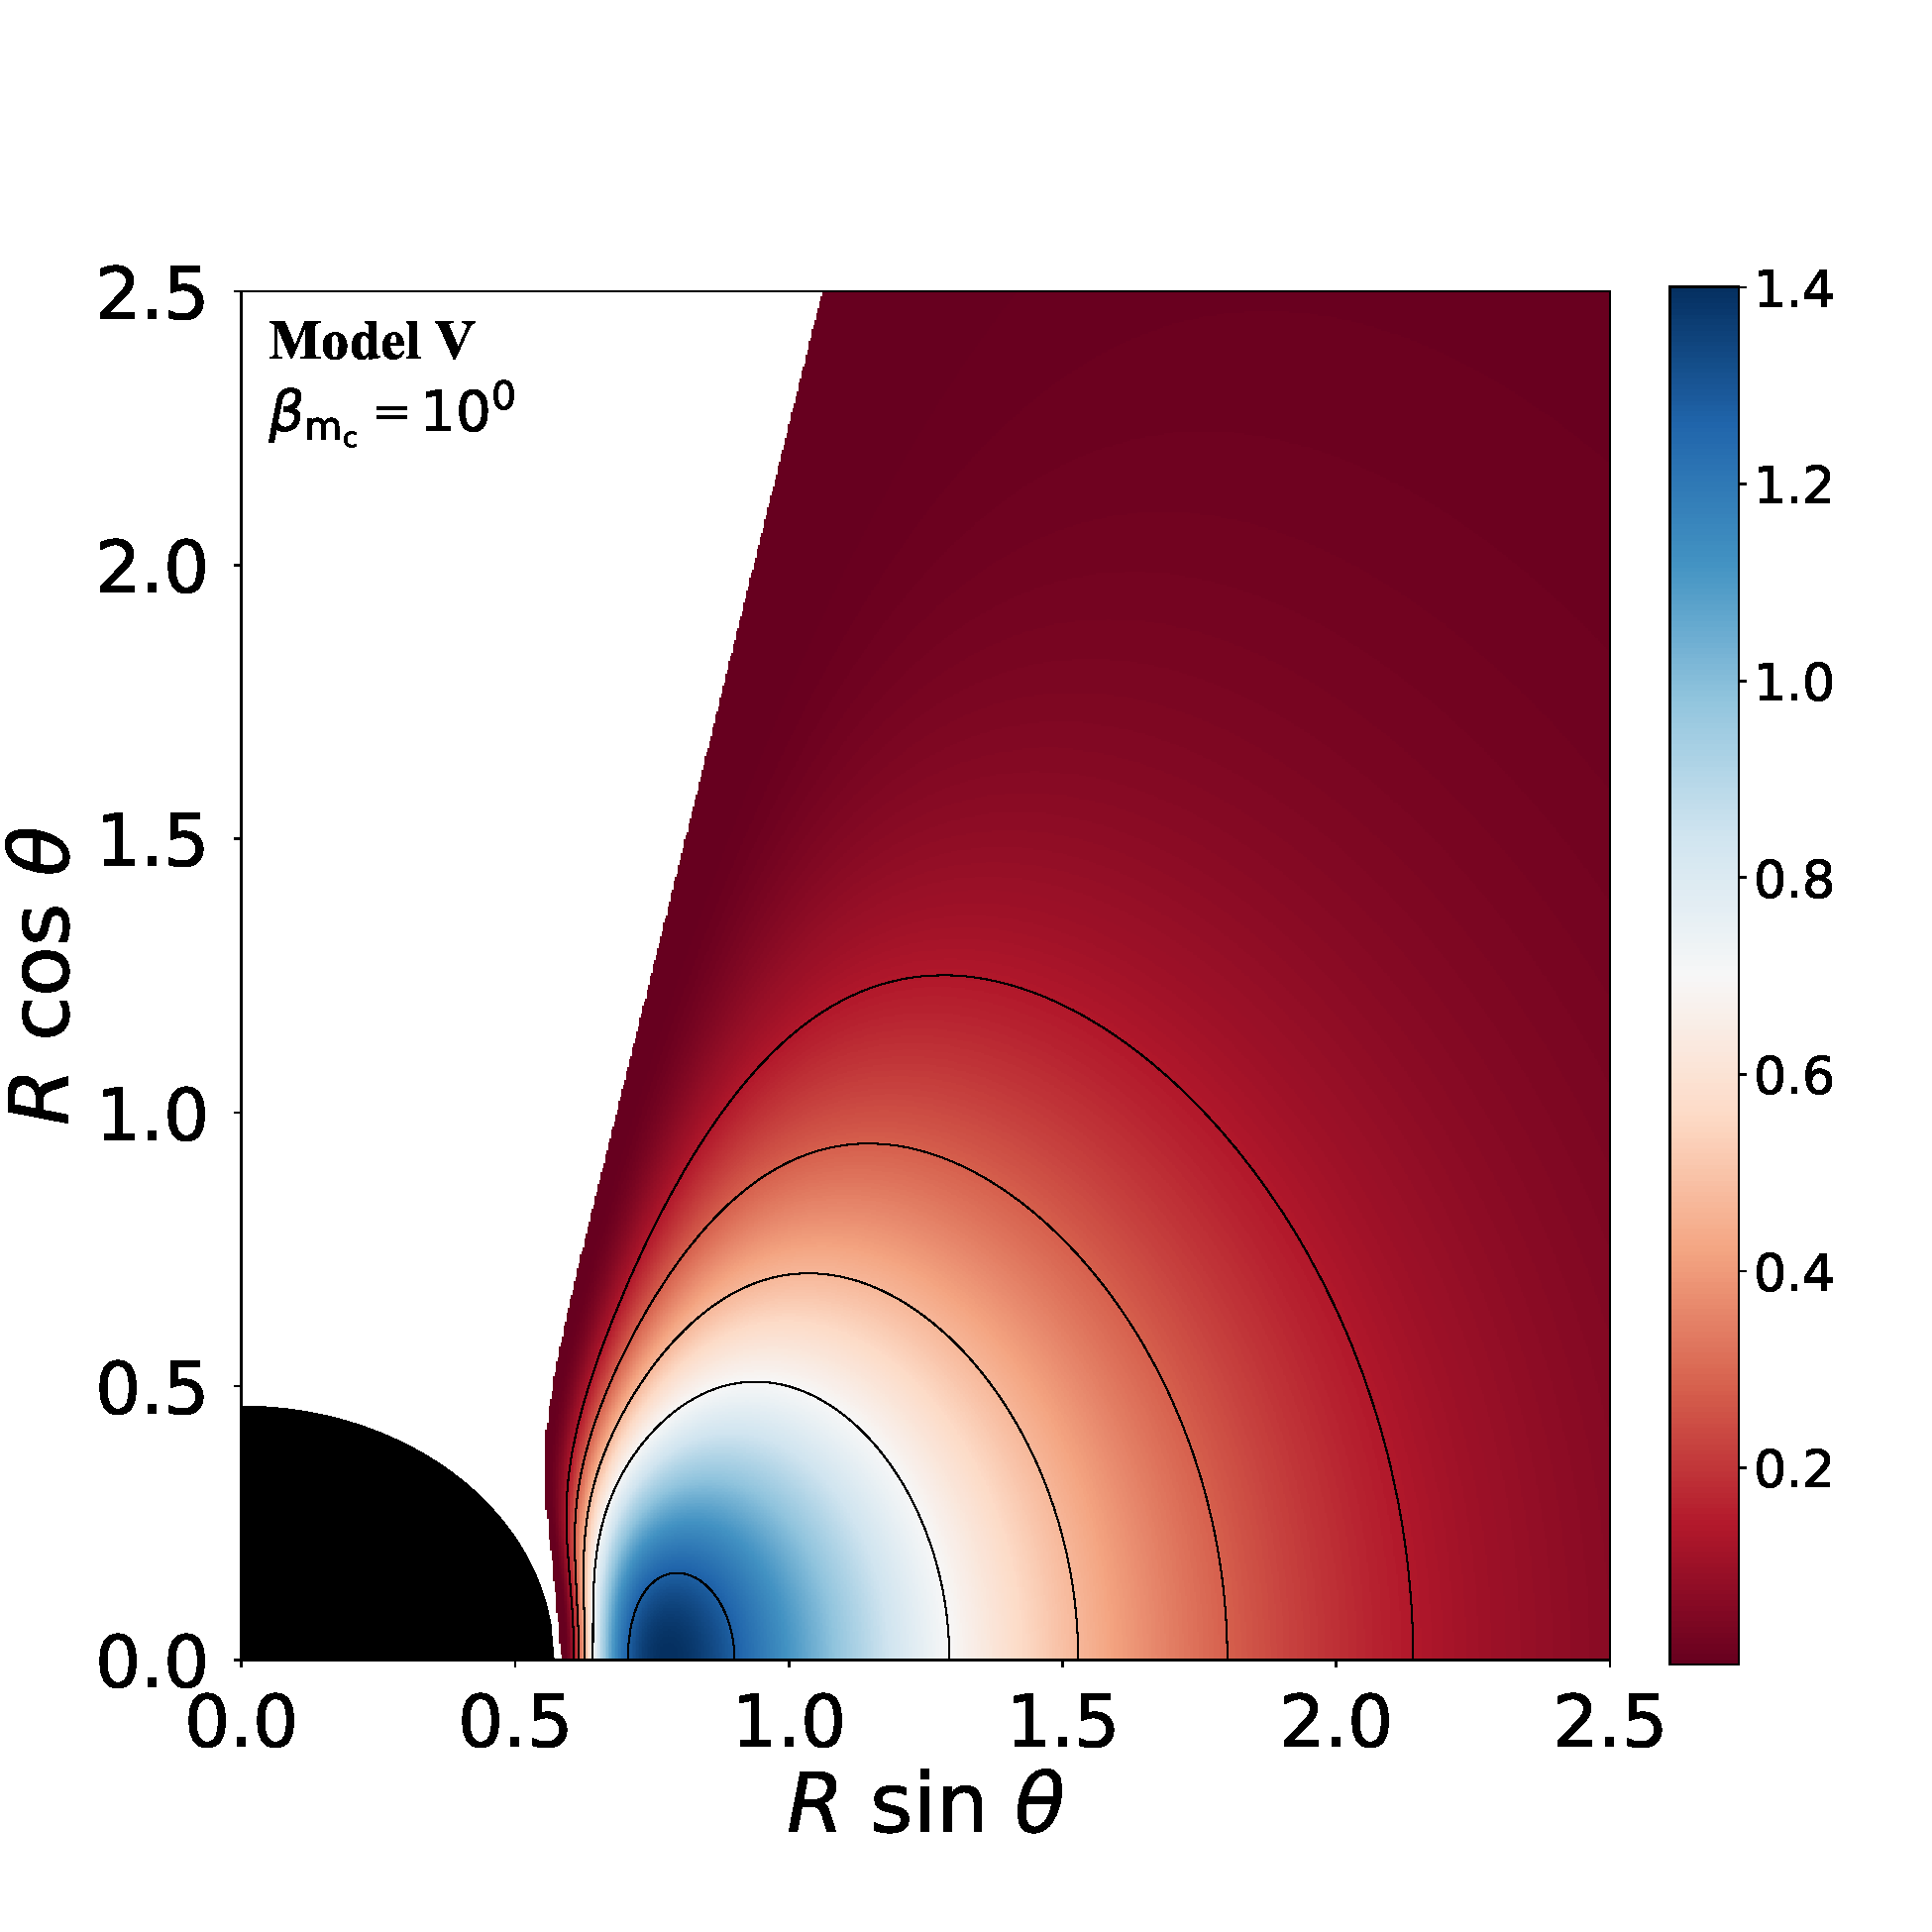
\includegraphics[scale=0.14]{figures/fig4_V_1.pdf}
\hspace{-0.2cm}
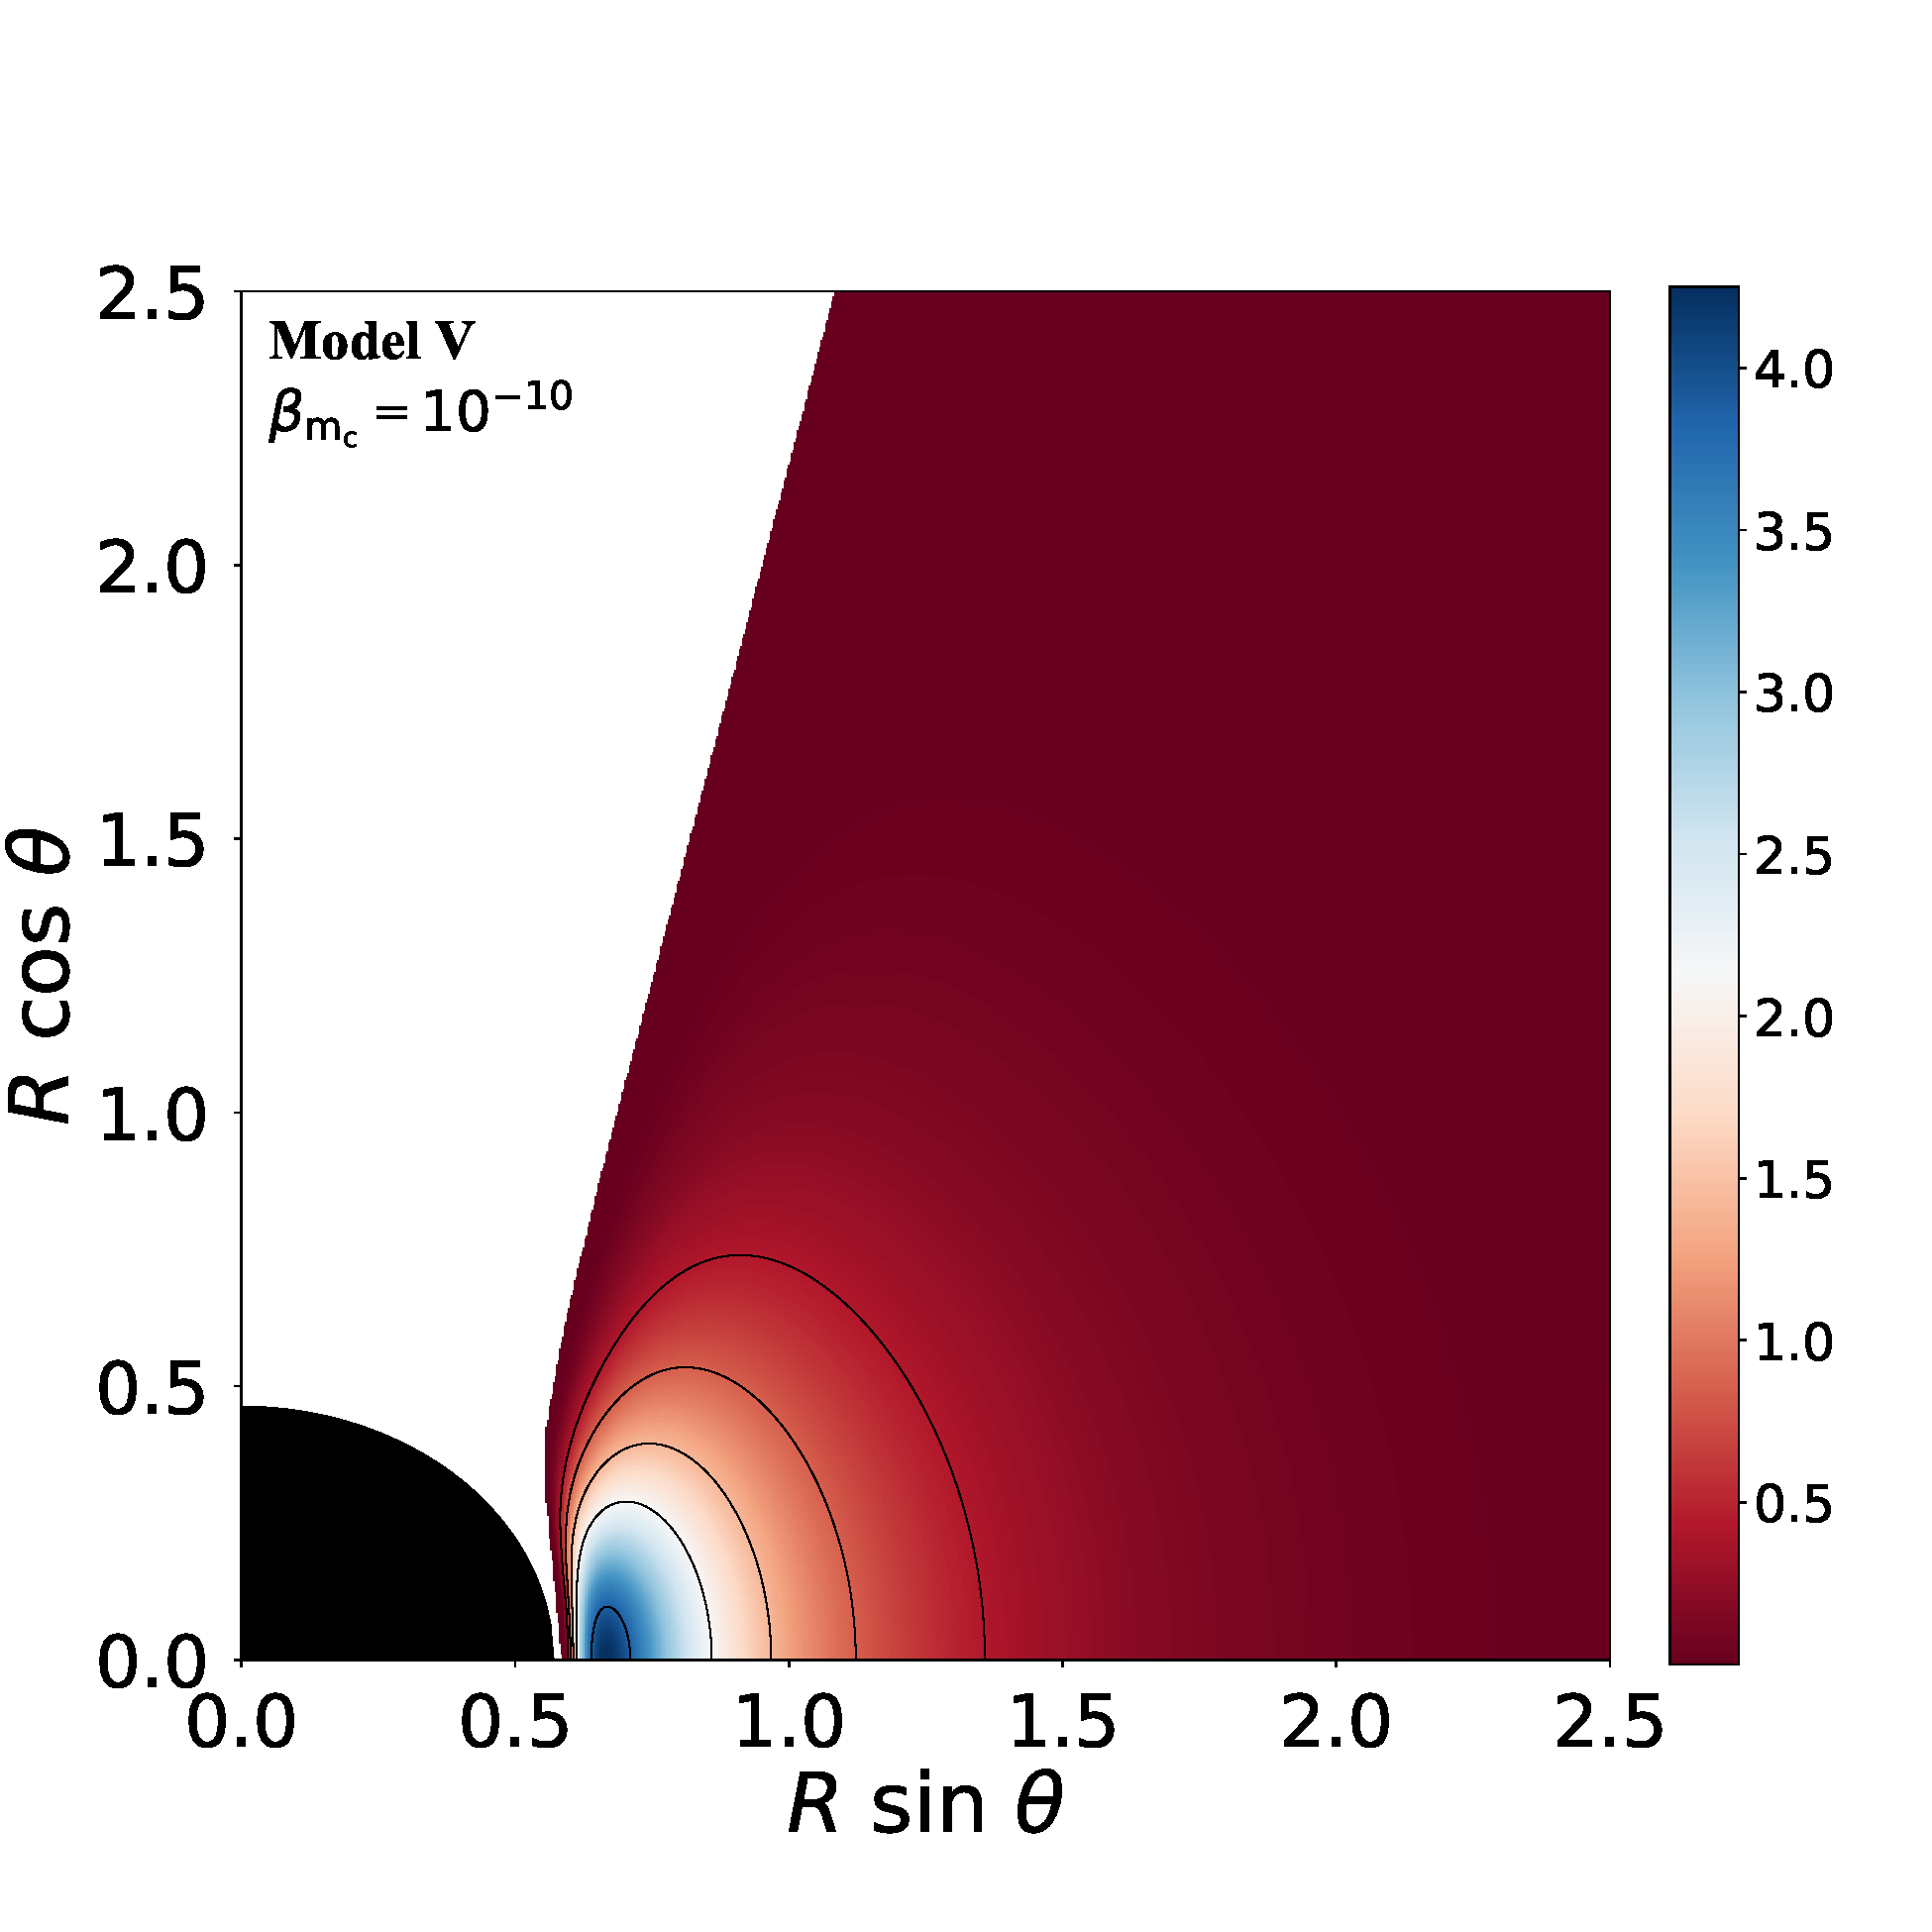
\includegraphics[scale=0.14]{figures/fig4_V__10.pdf}
\\
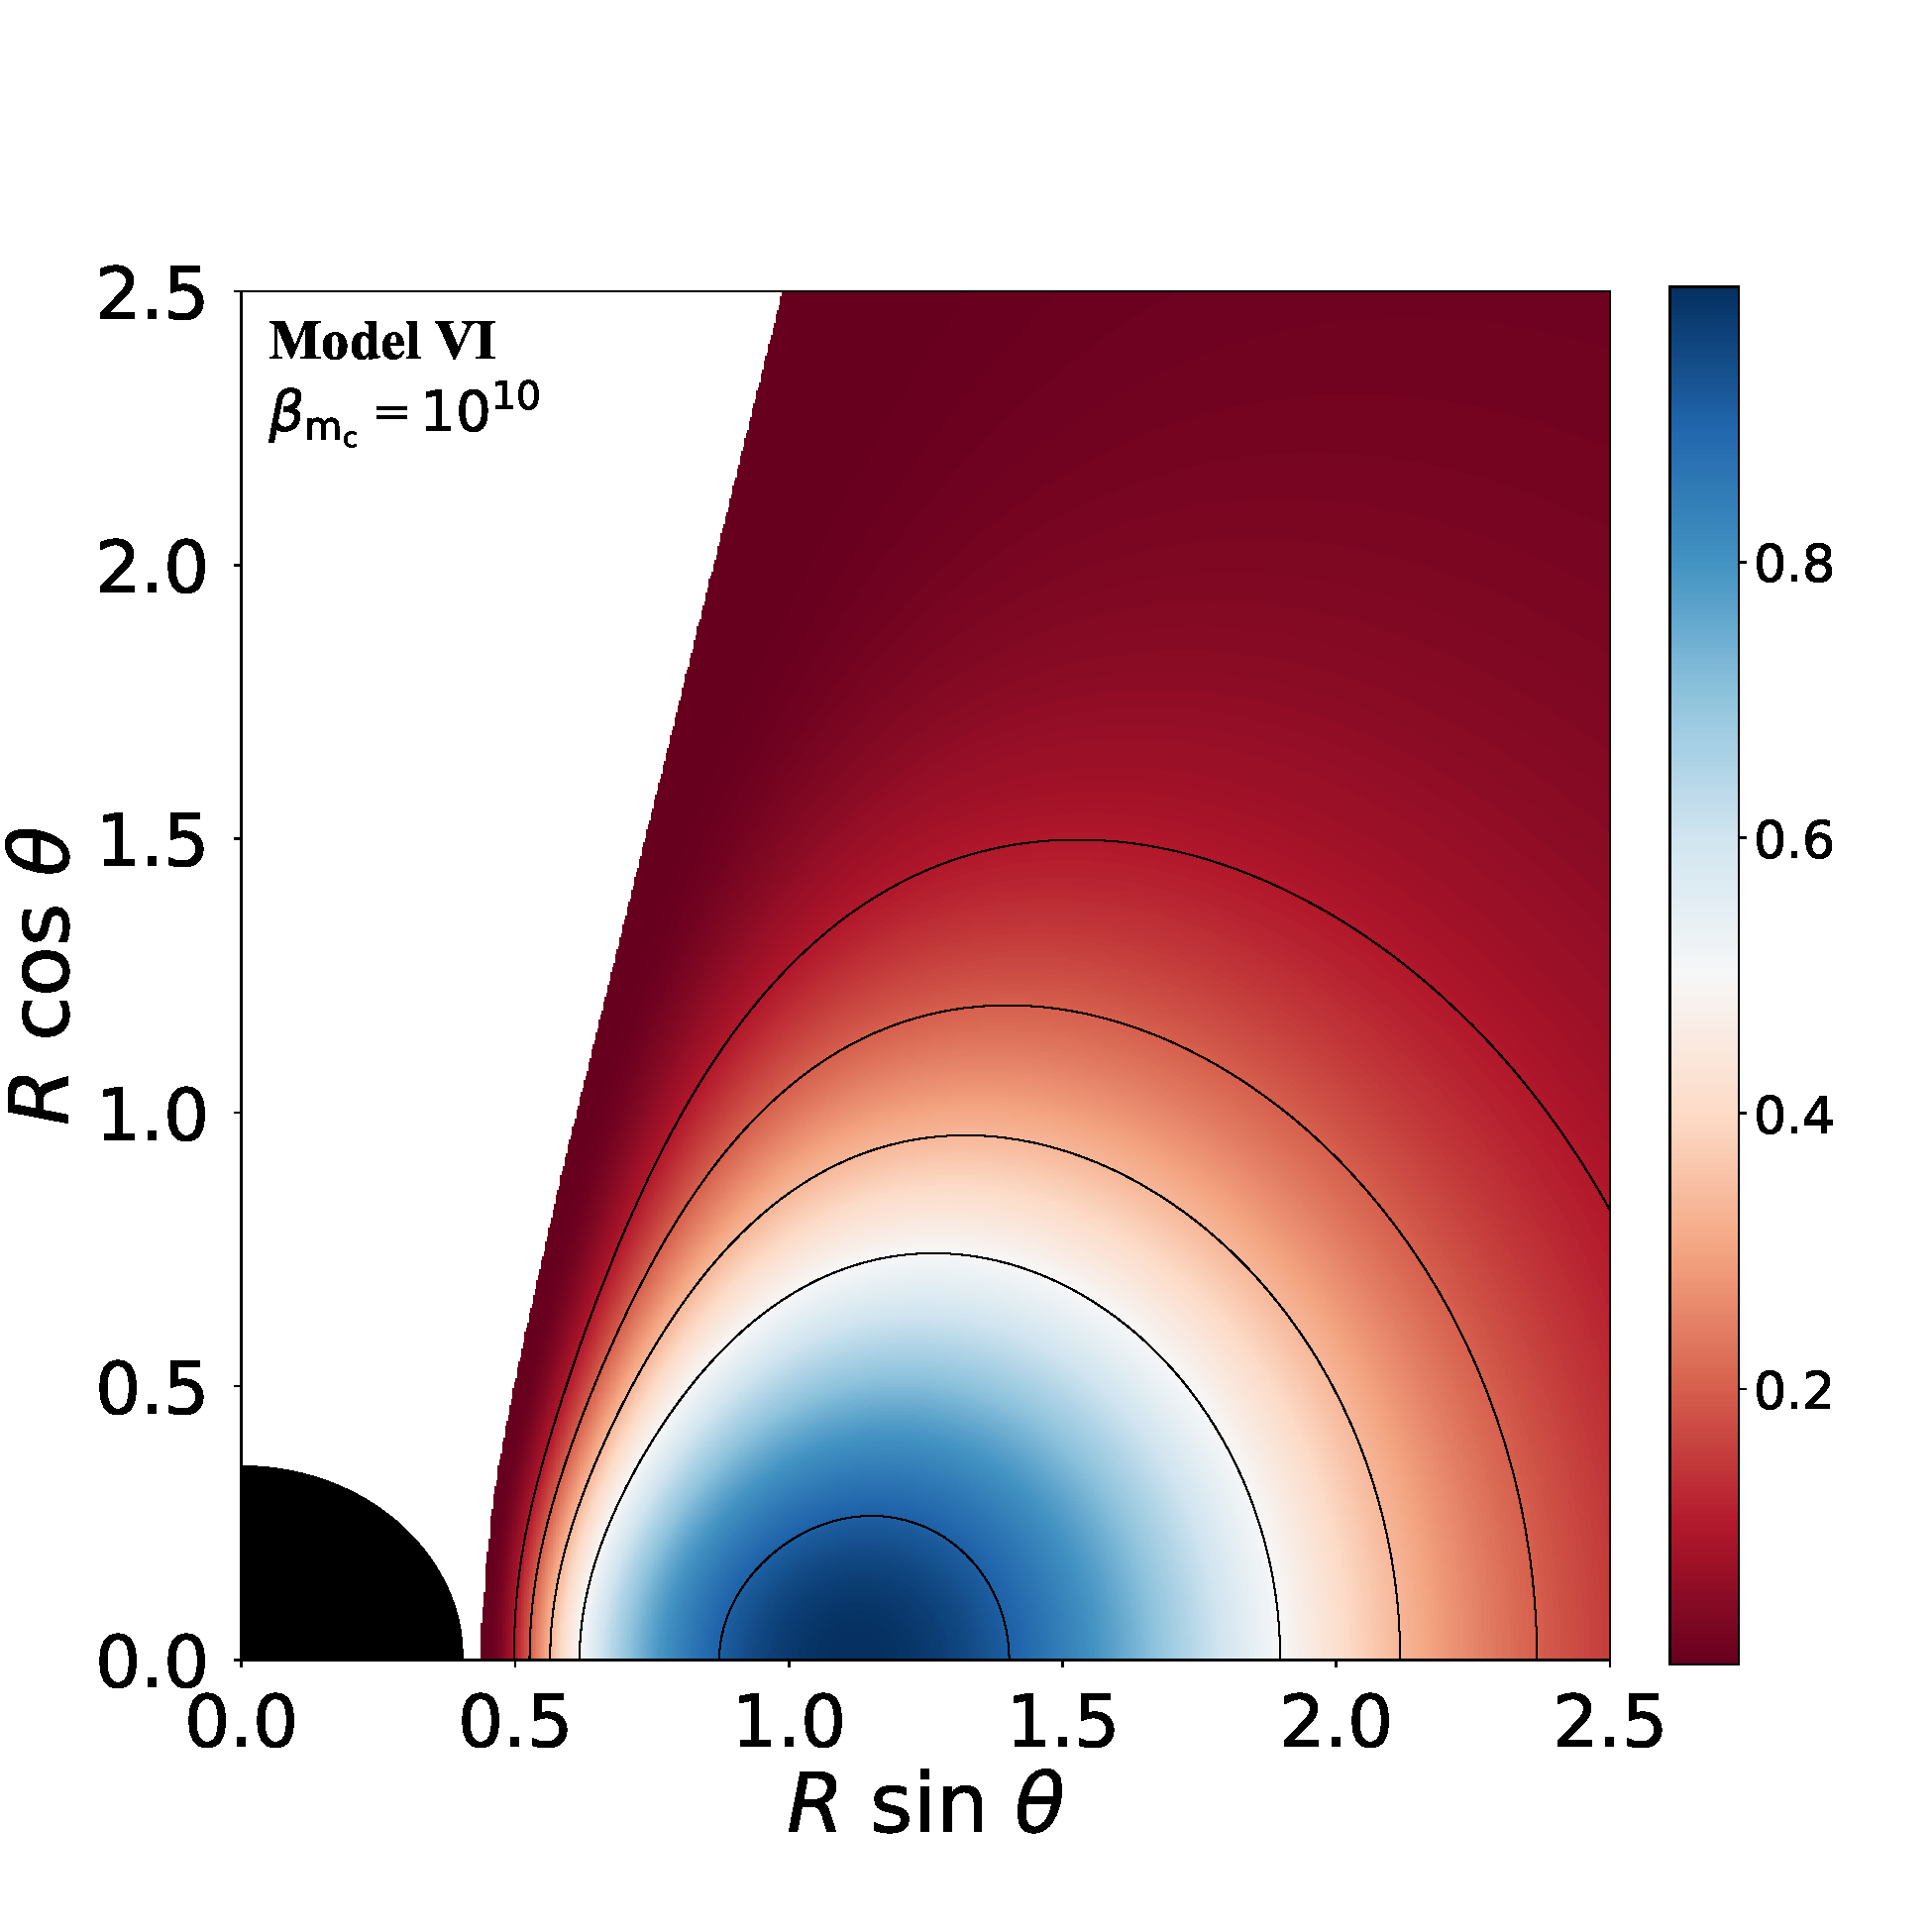
\includegraphics[scale=0.14]{figures/fig4_VI_10.pdf}
\hspace{-0.3cm}
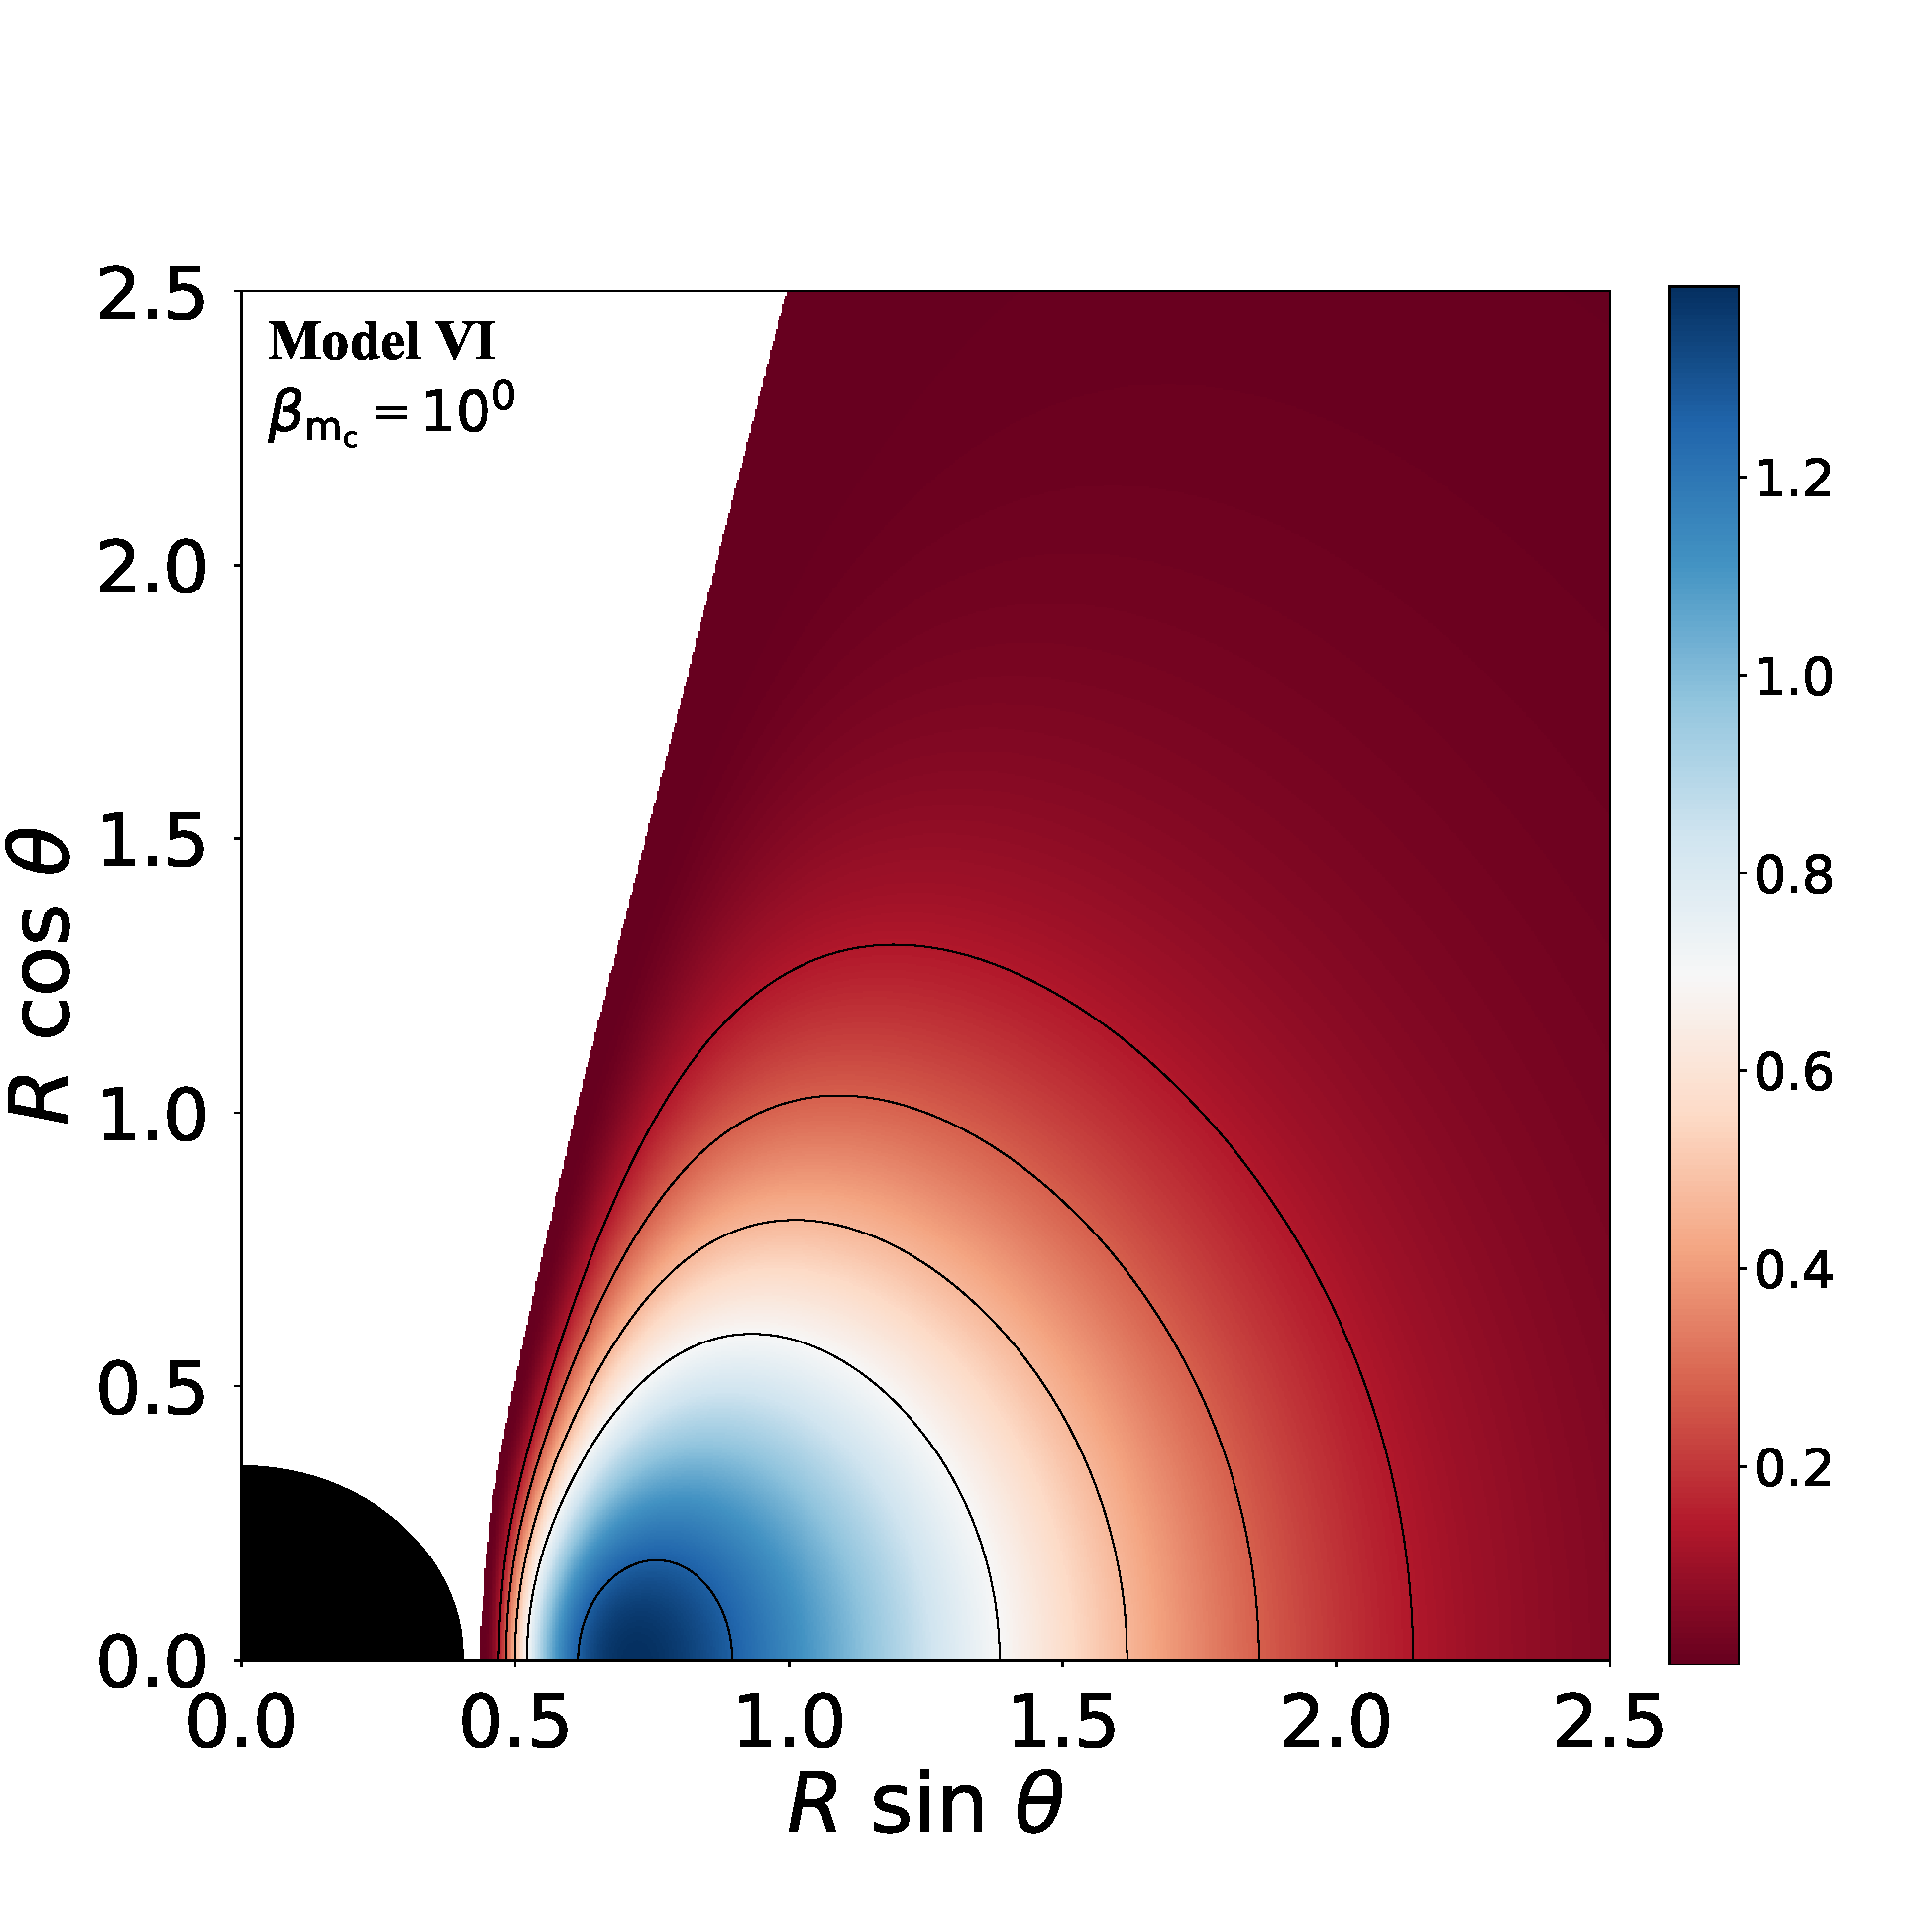
\includegraphics[scale=0.14]{figures/fig4_VI_1.pdf}
\hspace{-0.2cm}
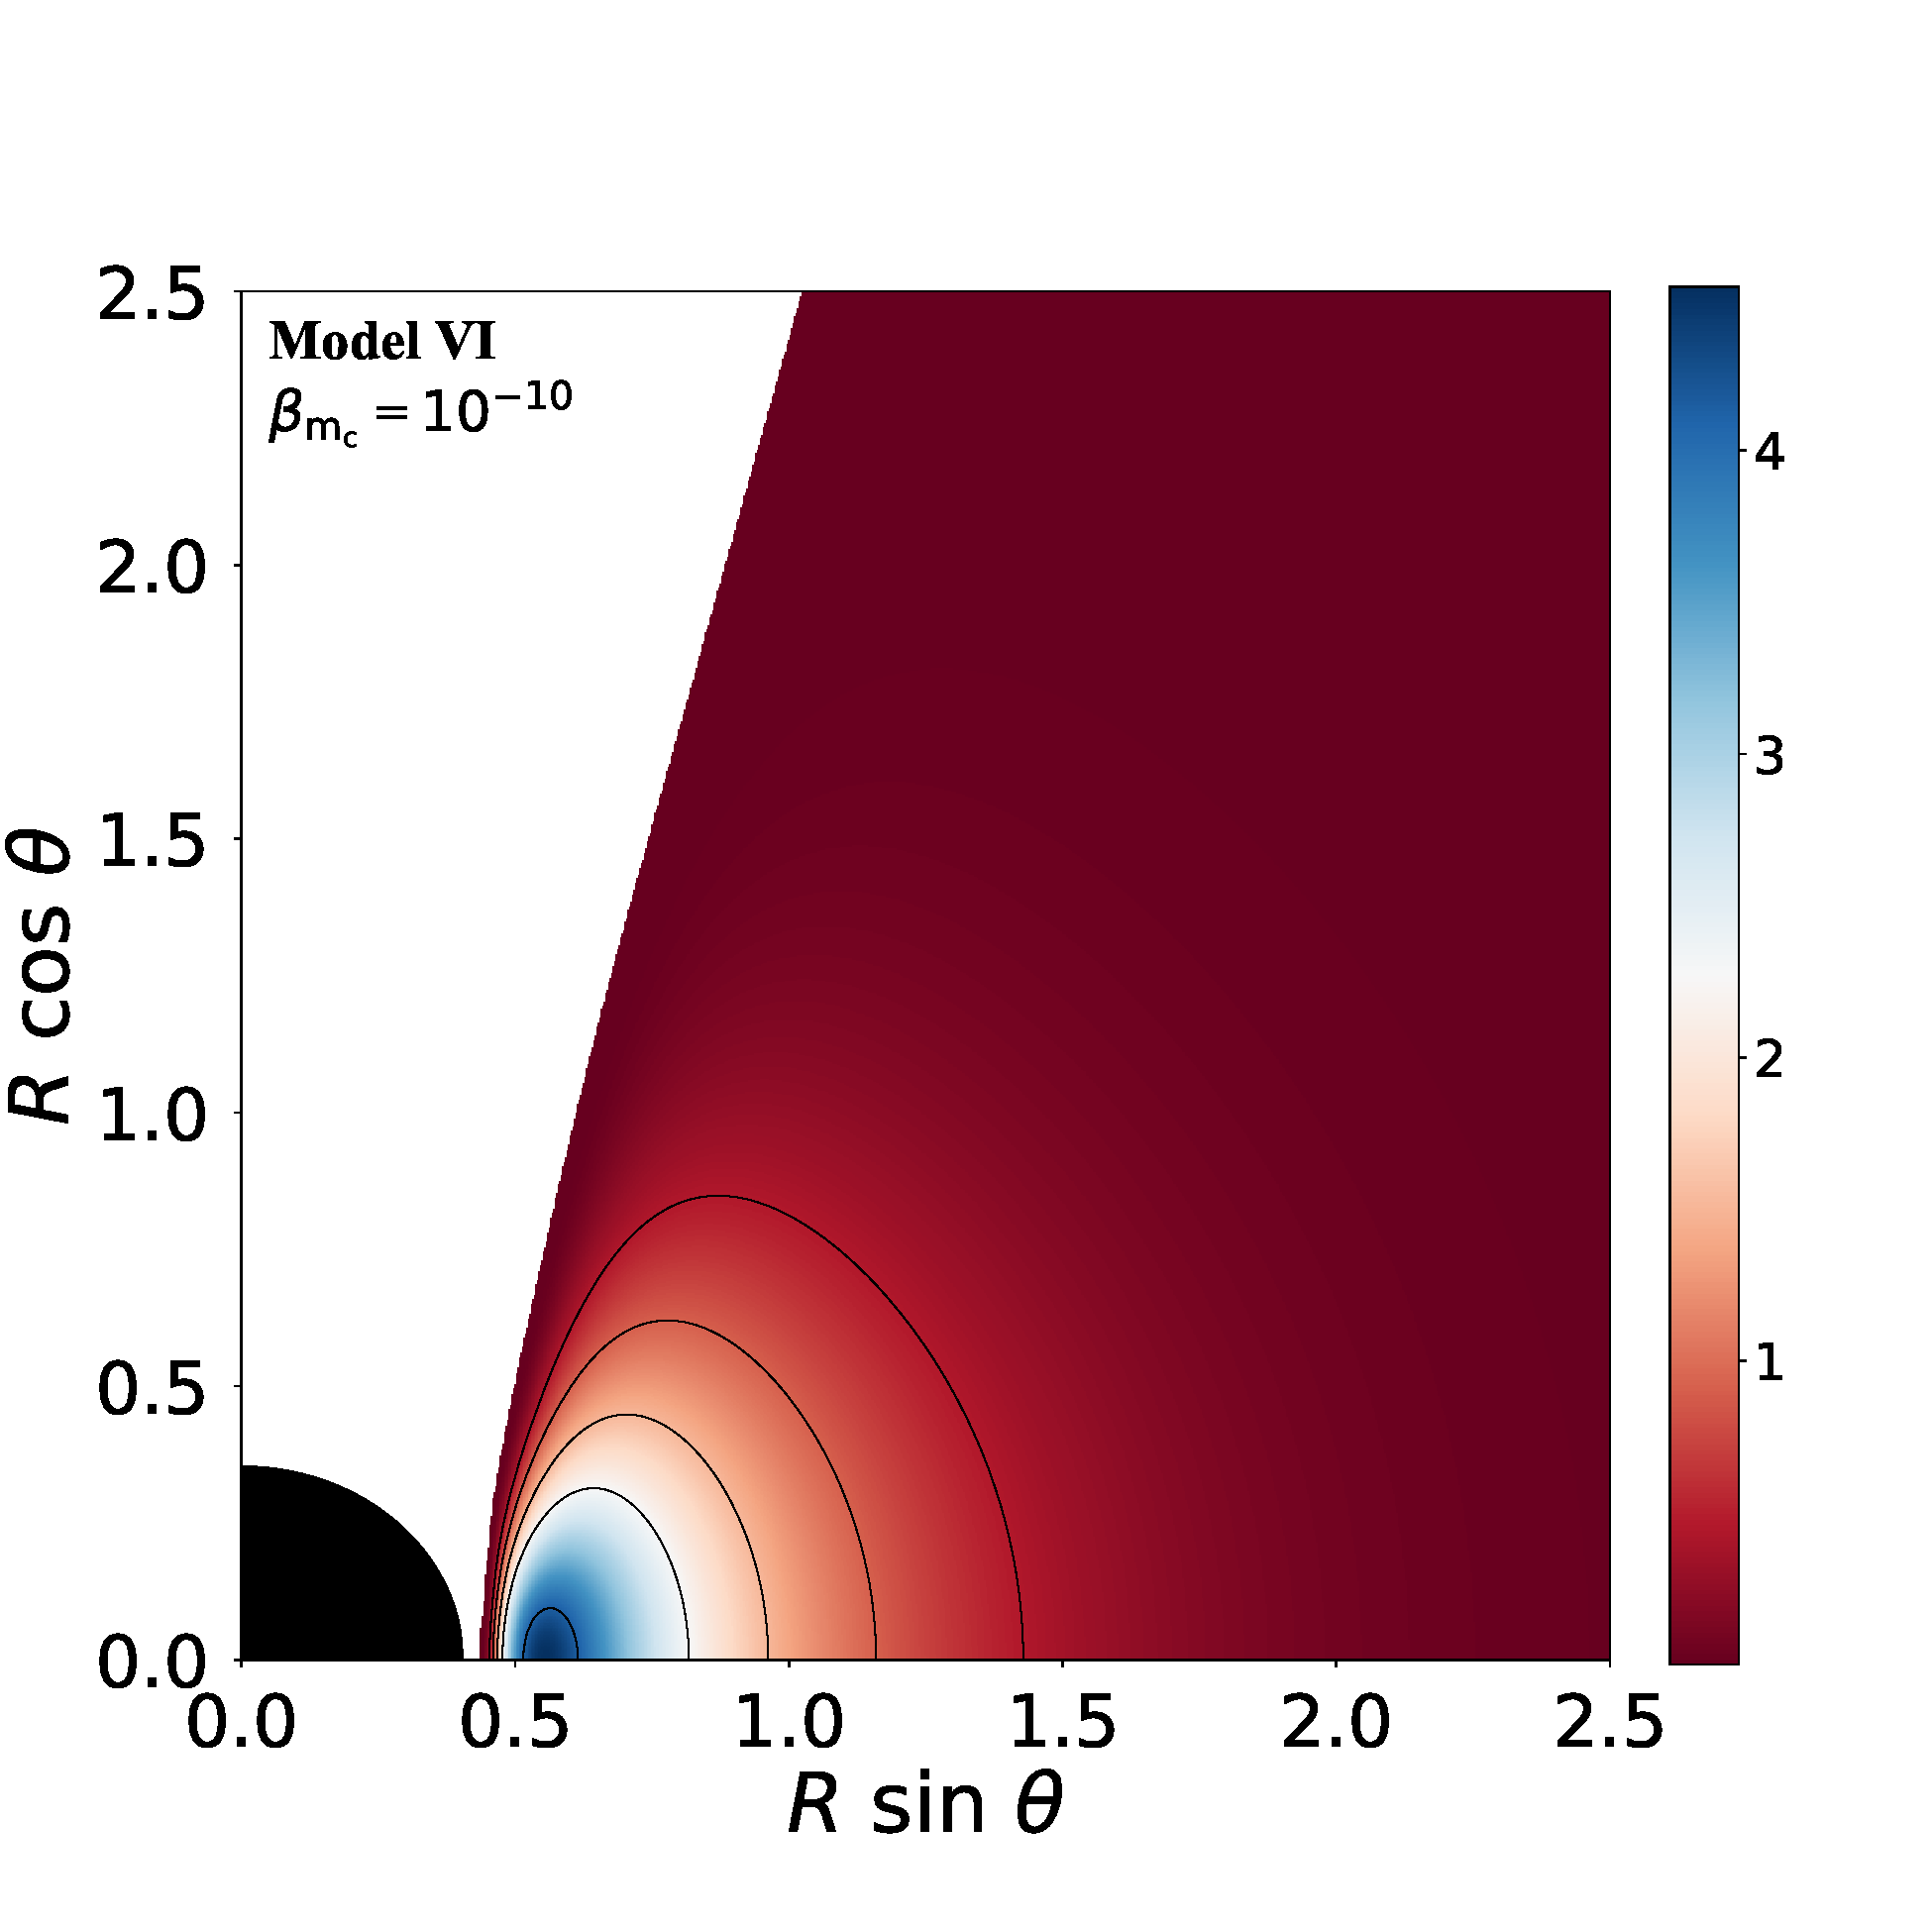
\includegraphics[scale=0.14]{figures/fig4_VI__10.pdf}
\\
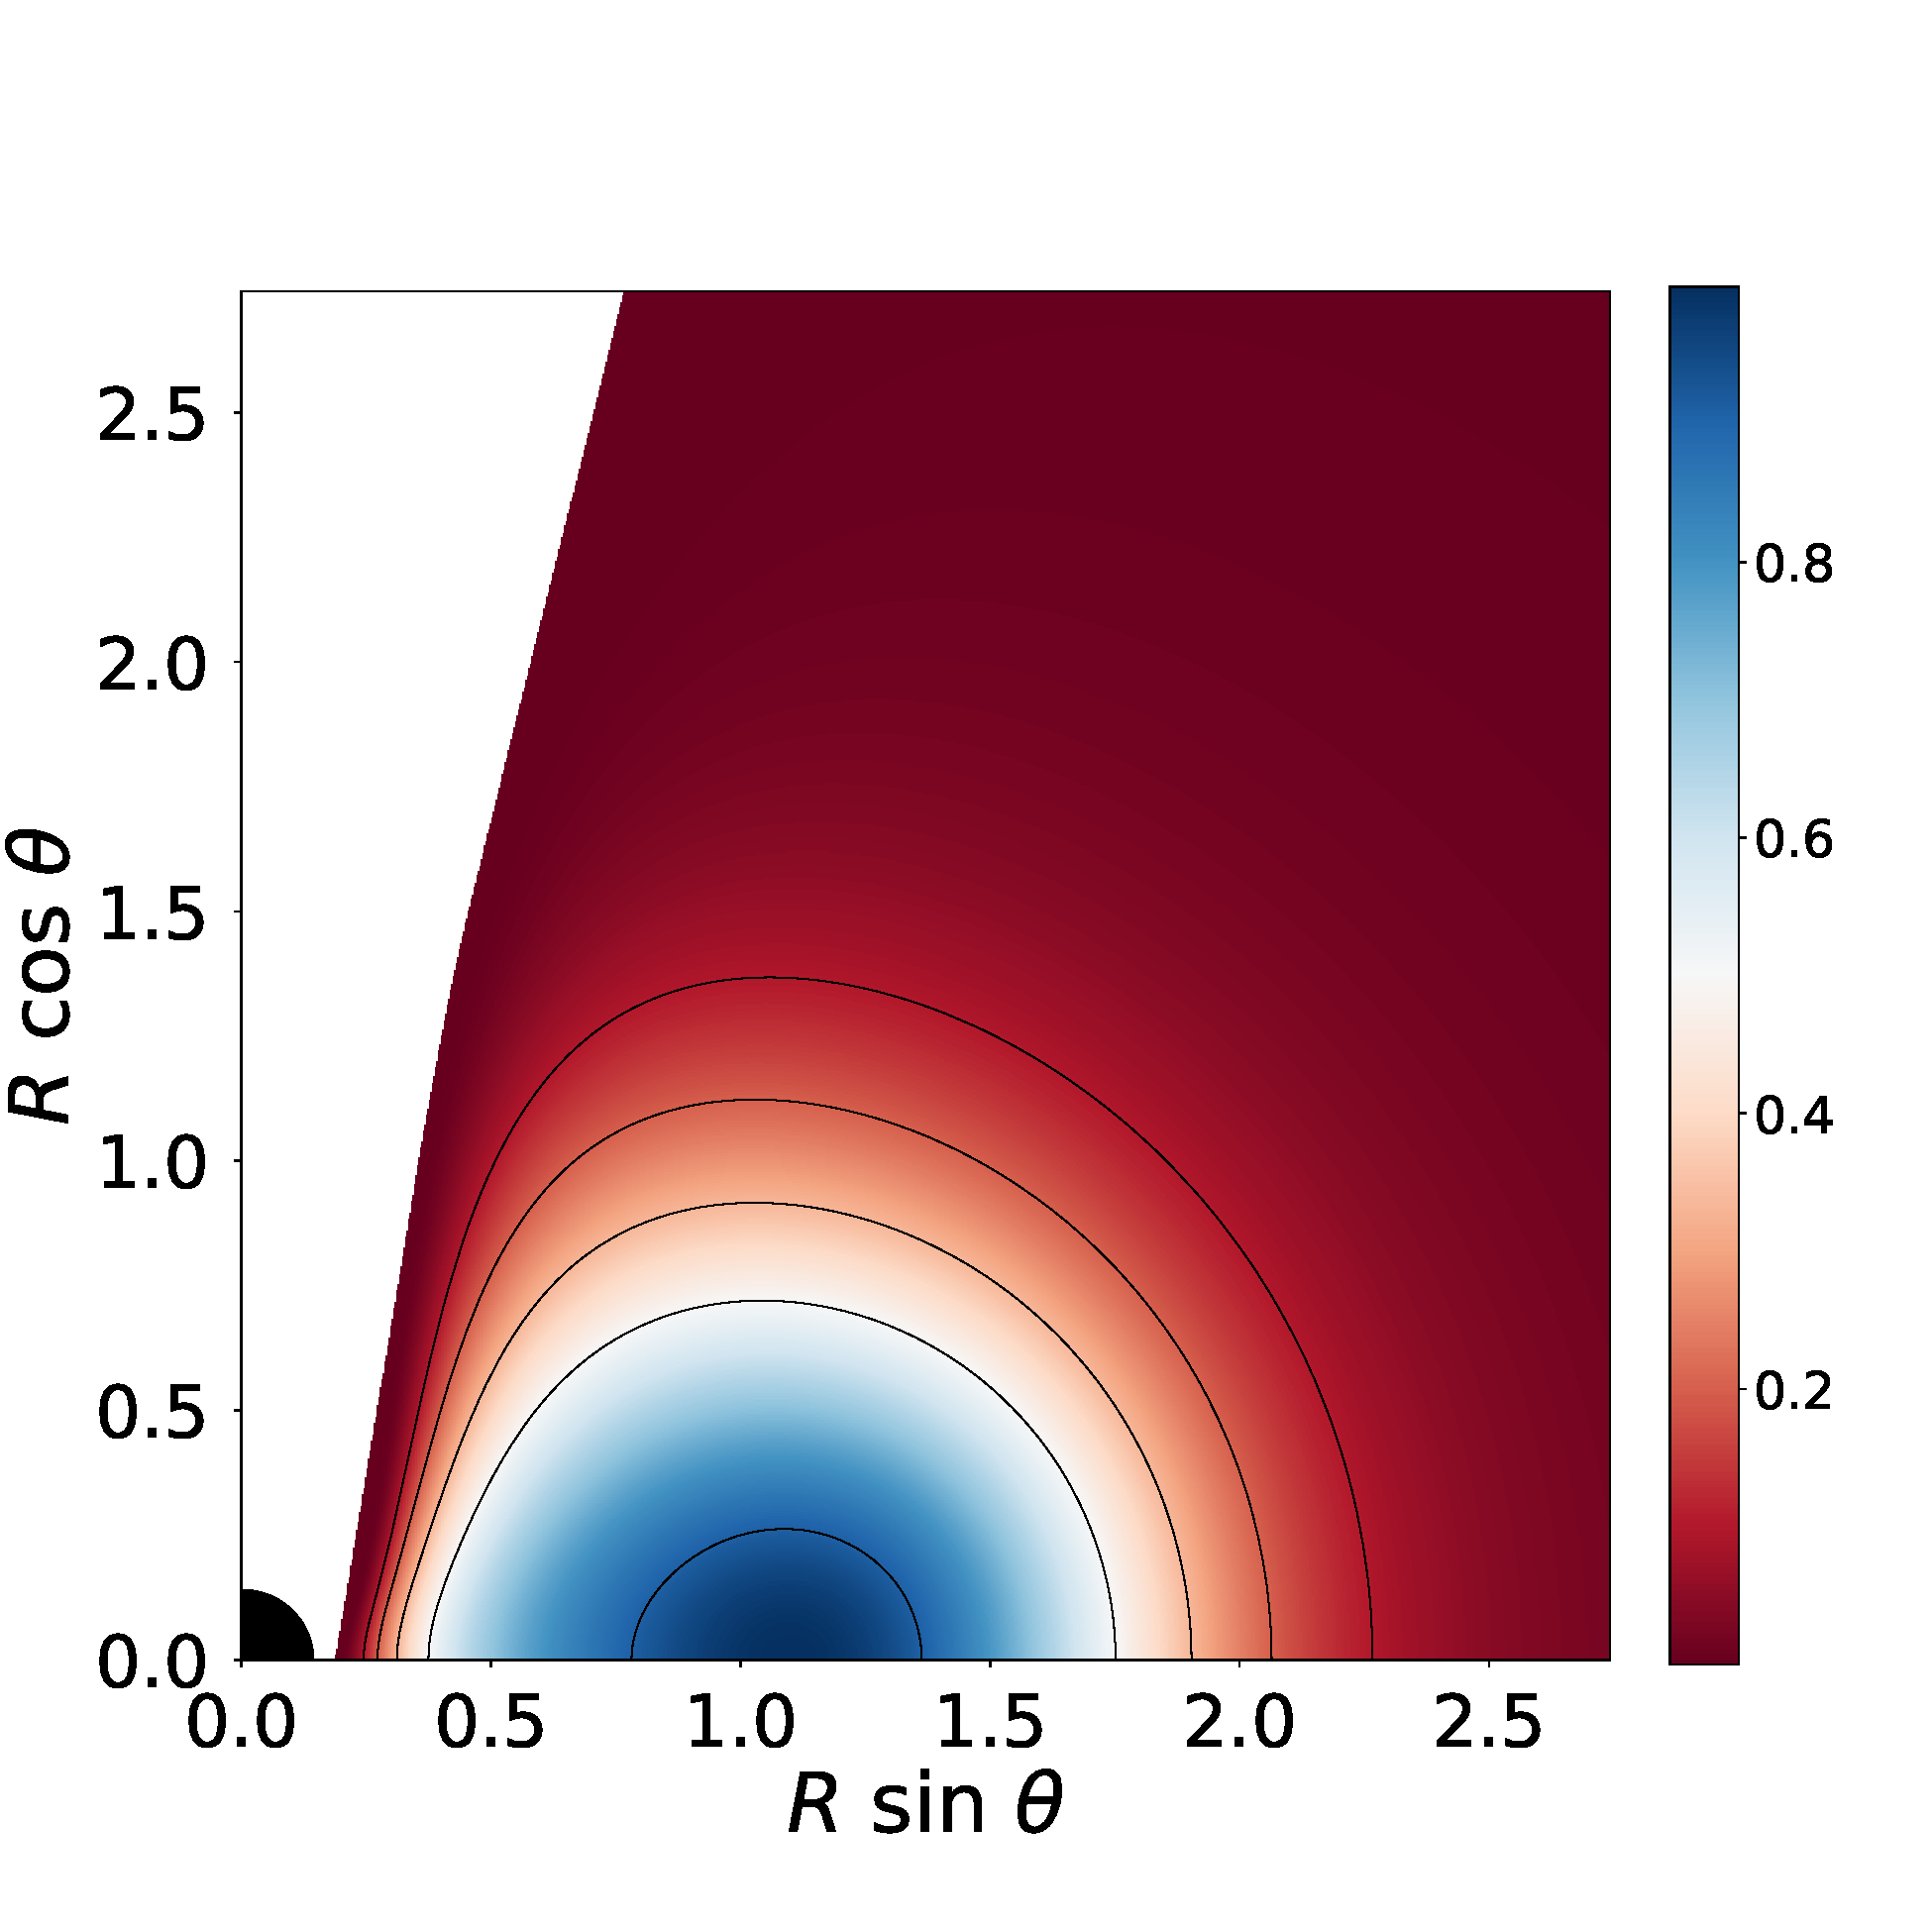
\includegraphics[scale=0.14]{figures/fig4_VII_10.pdf}
\hspace{-0.3cm}
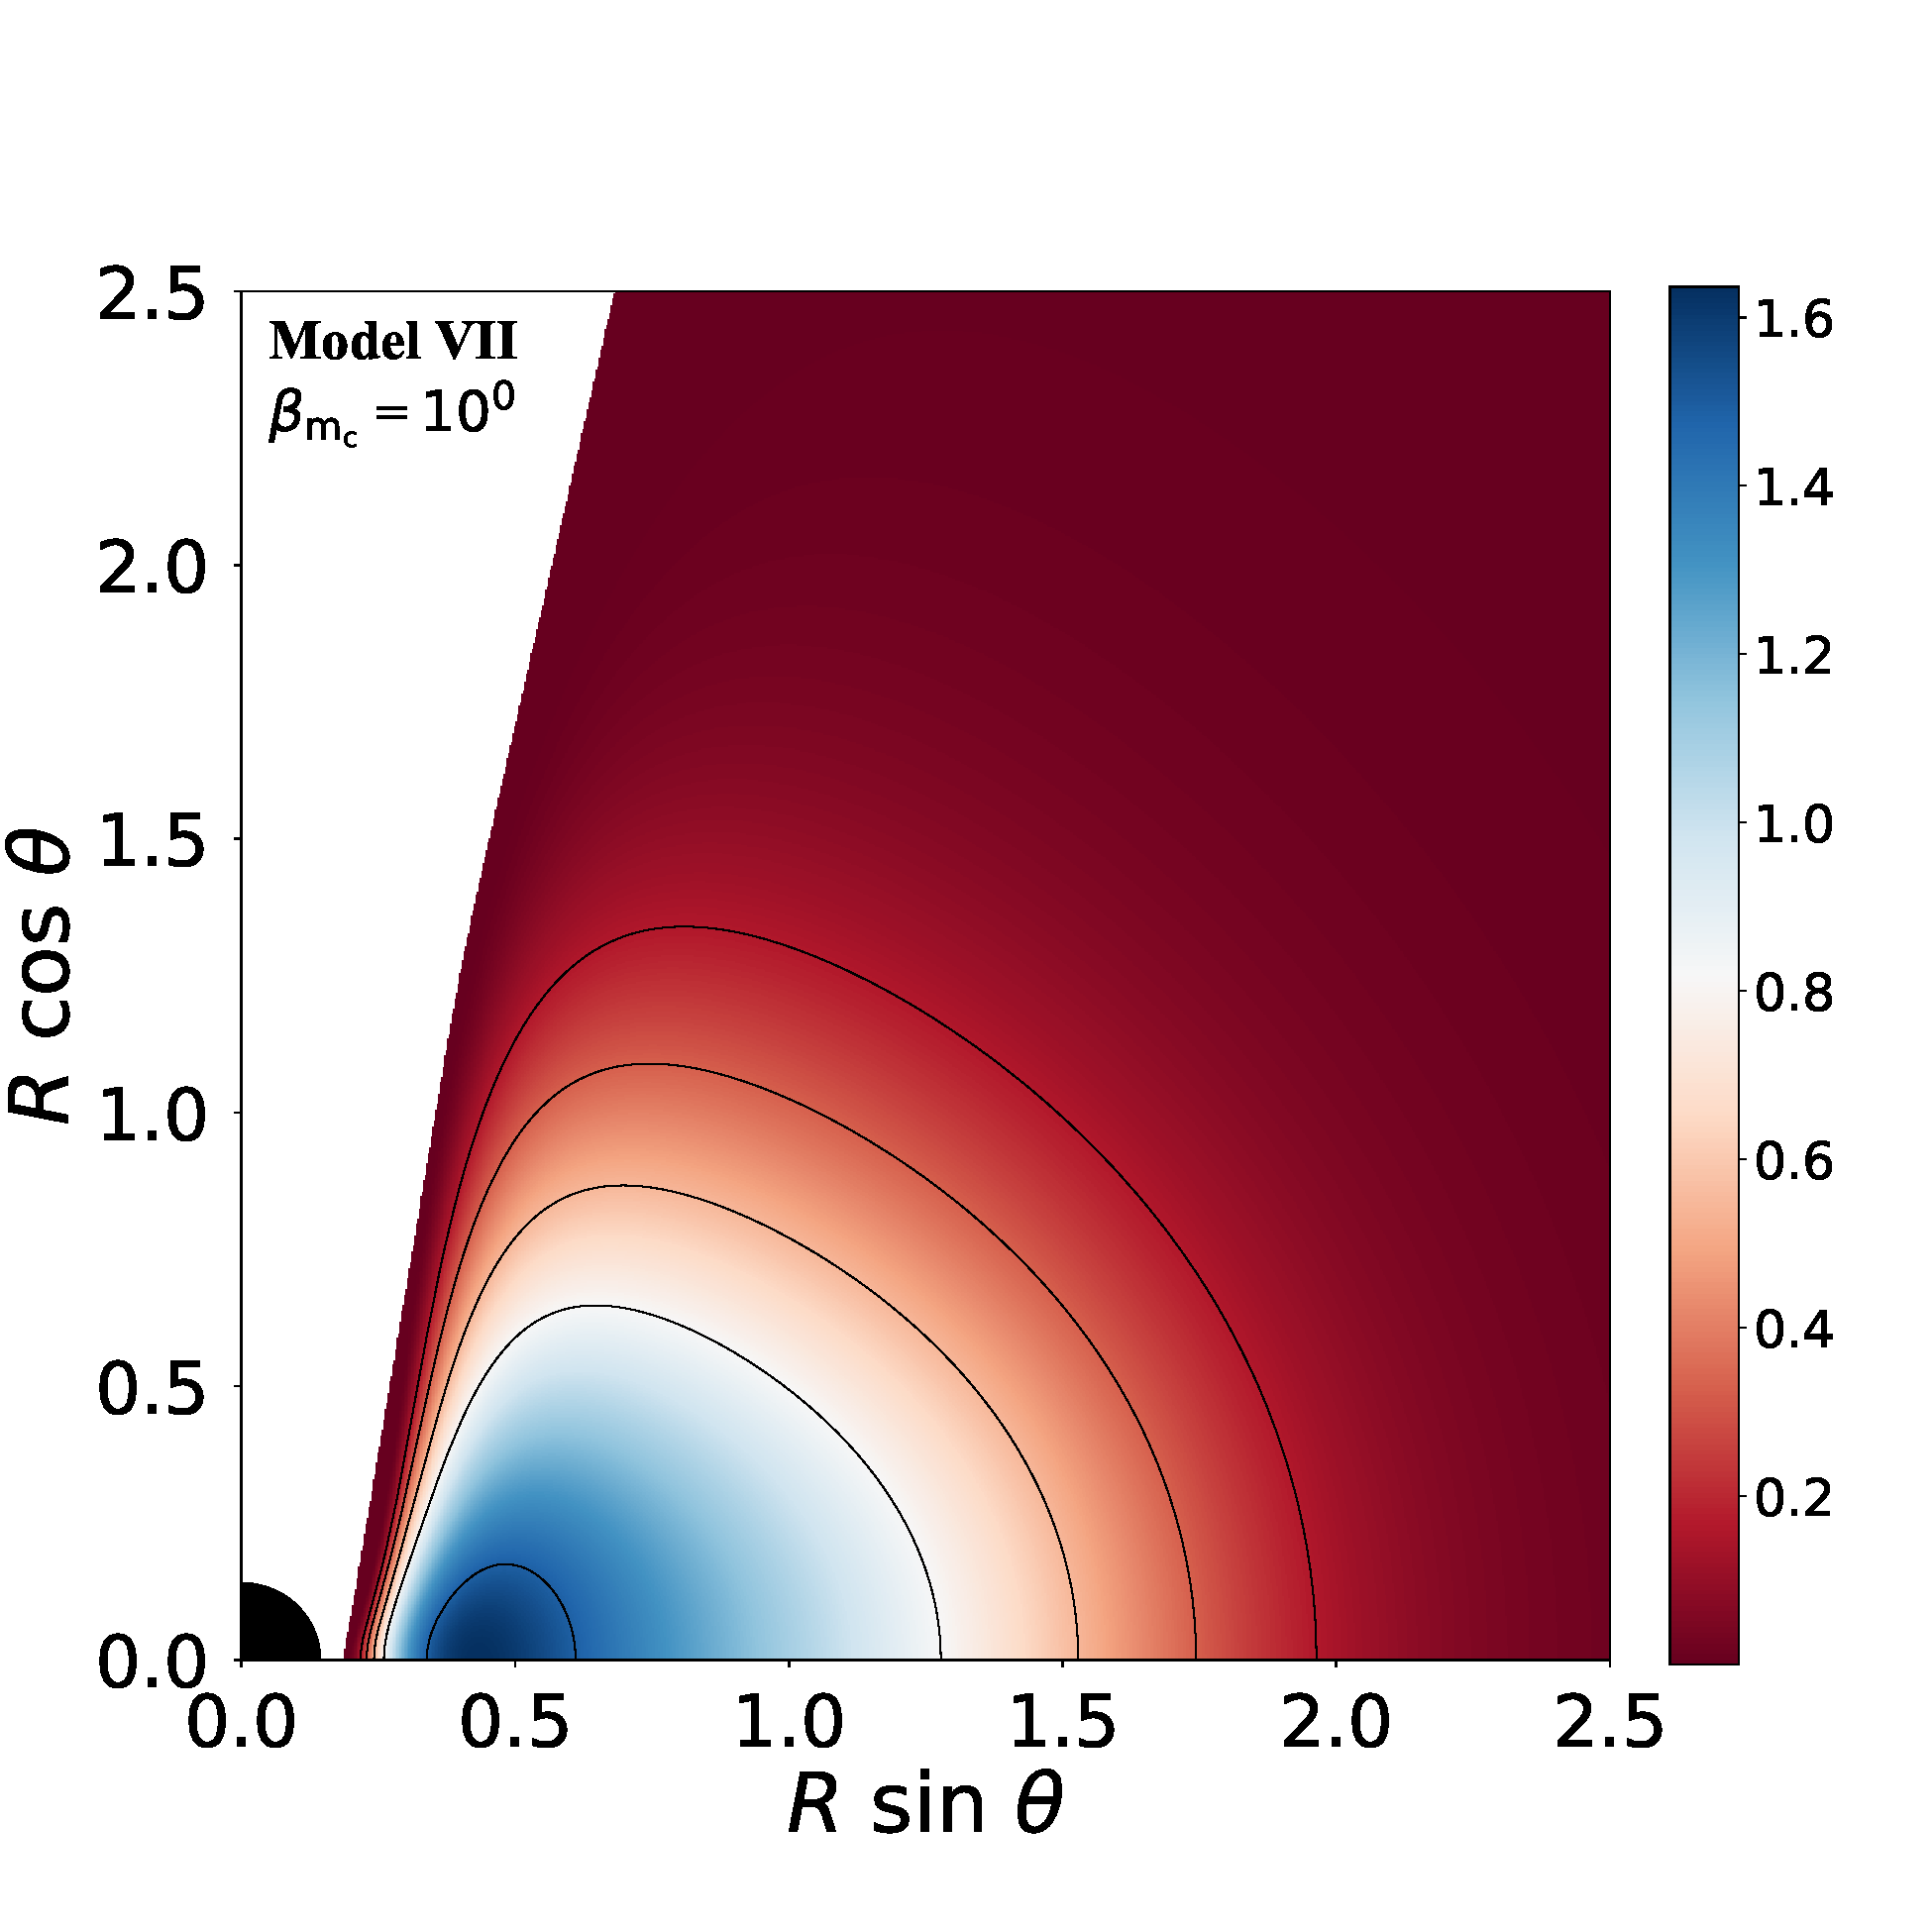
\includegraphics[scale=0.14]{figures/fig4_VII_1.pdf}
\hspace{-0.2cm}
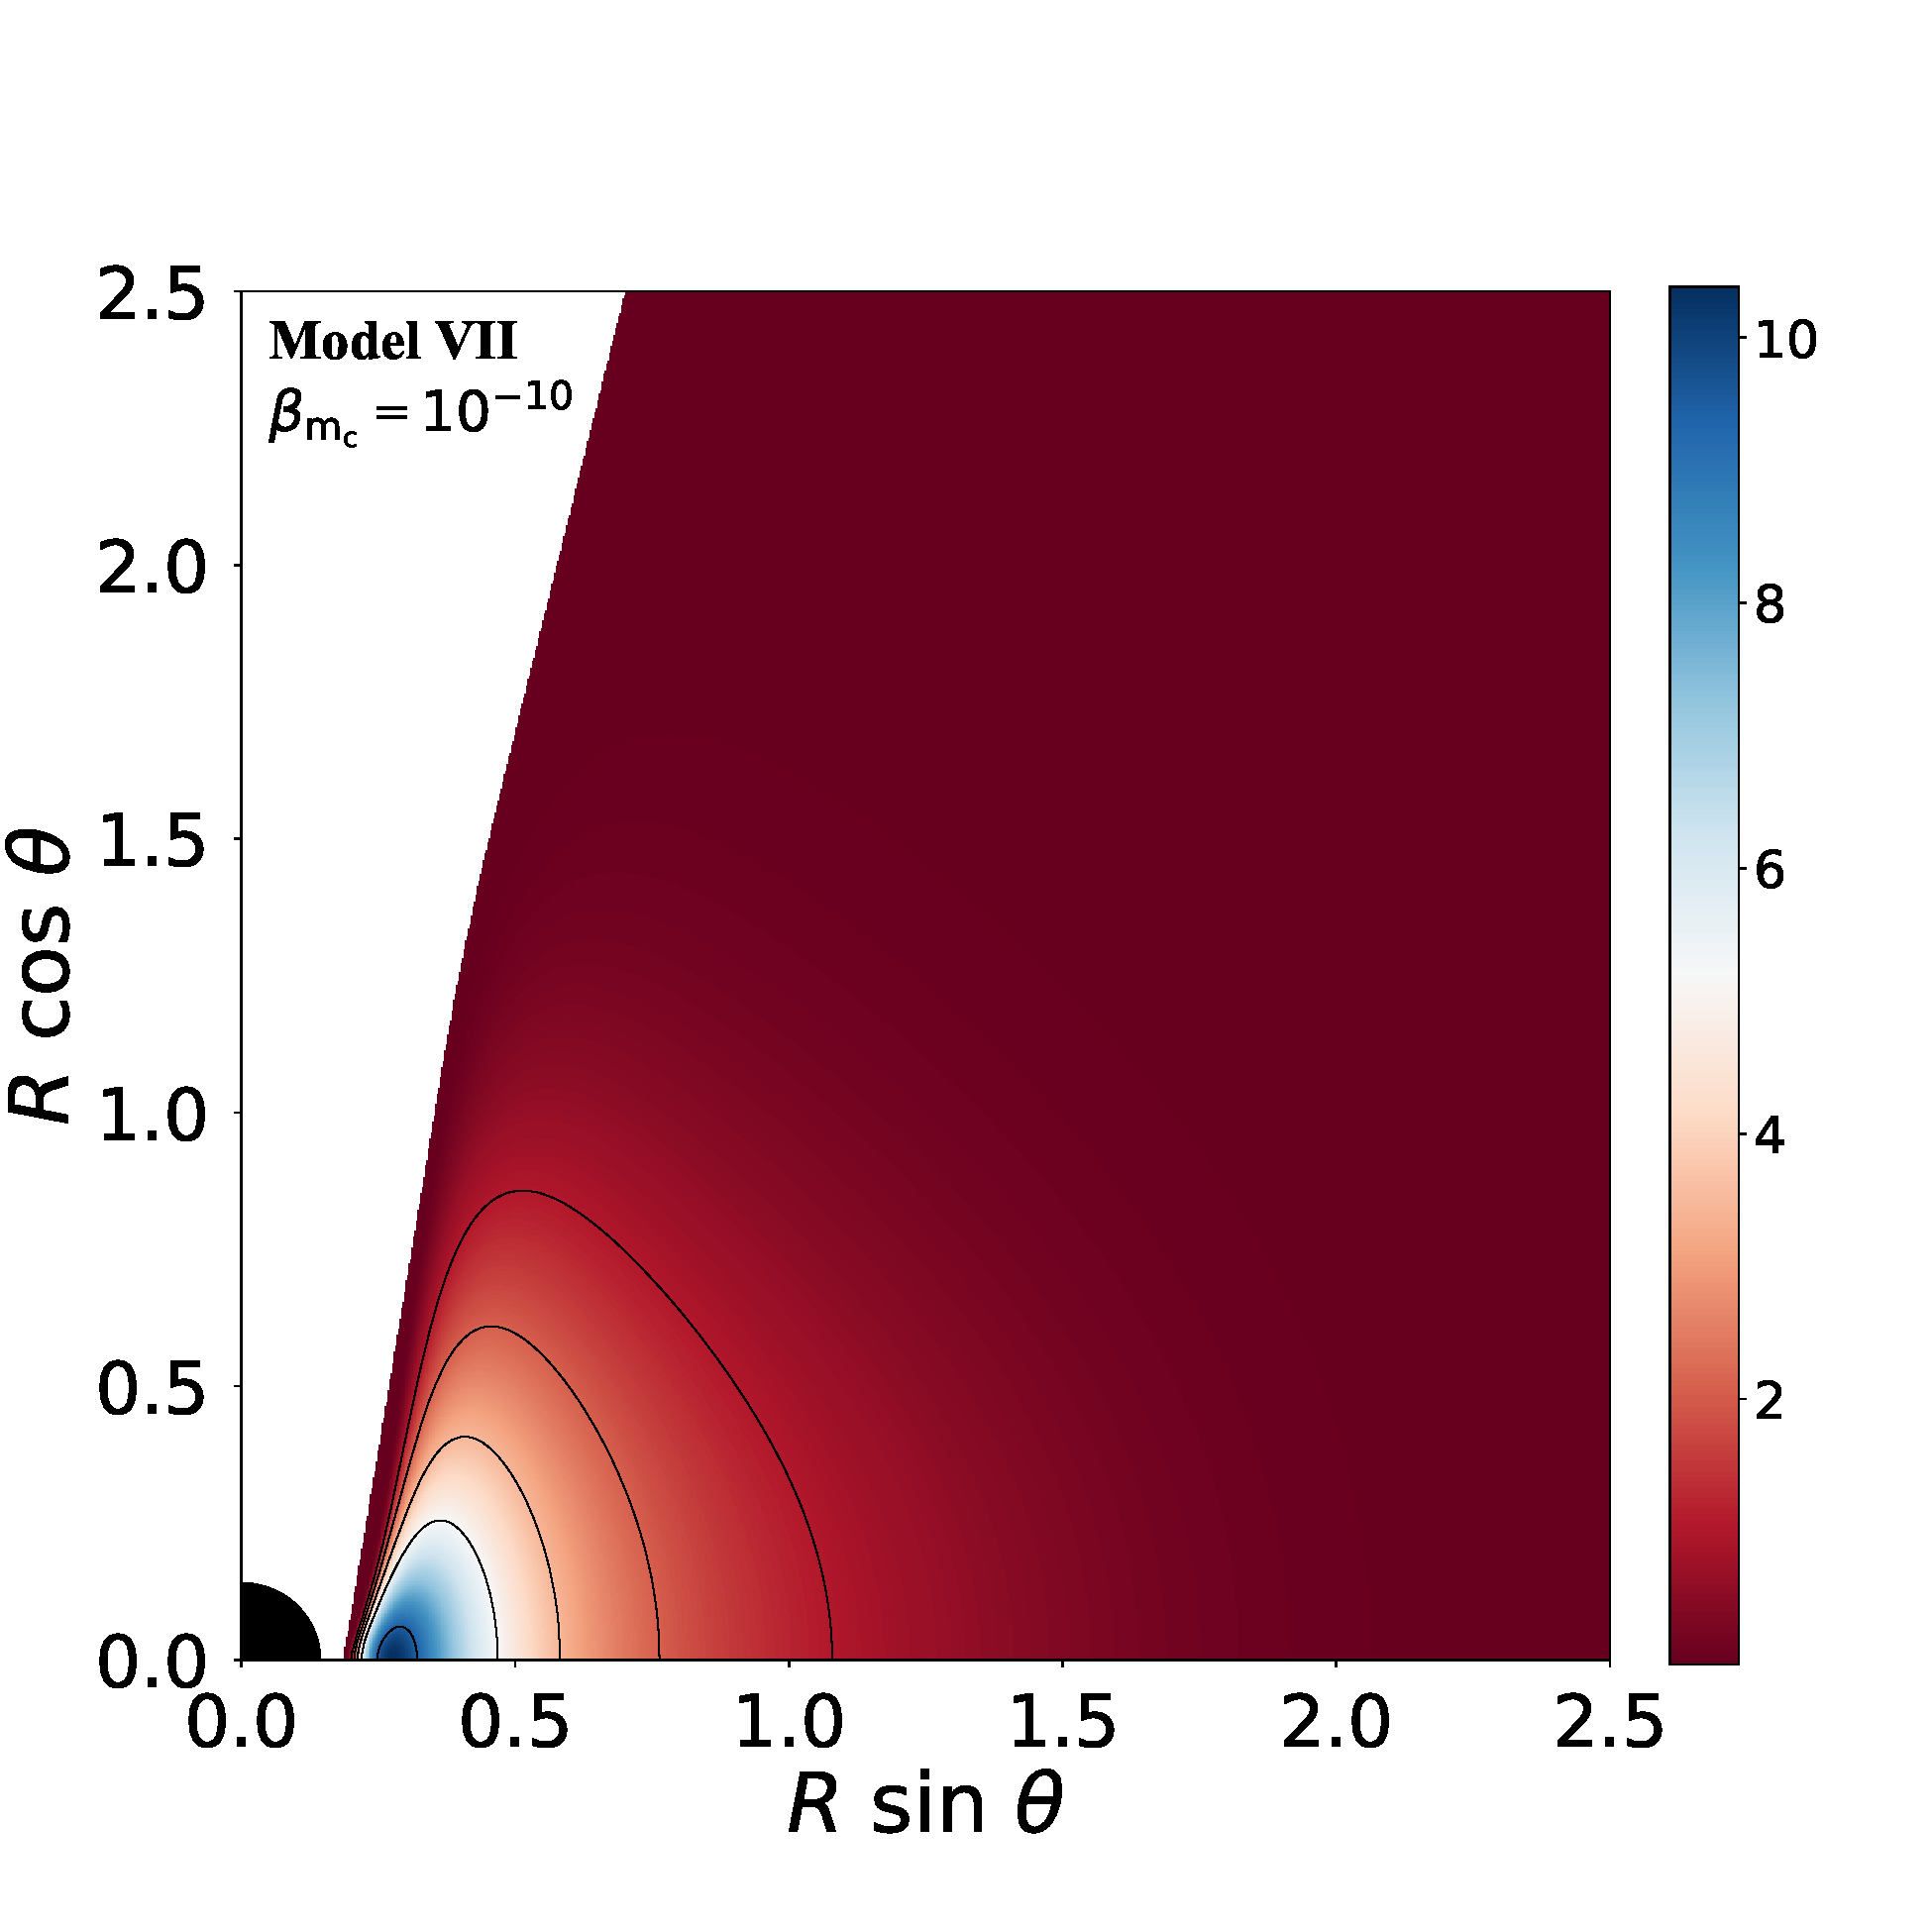
\includegraphics[scale=0.14]{figures/fig4_VII__10.pdf}
\hspace{-0.2cm}
\caption{Same as Fig.~\ref{models_II} but using the perimetral radial coordinate $R$.}
\label{models_peri_II}
\end{figure*}

%%%%%%%%%%%%
\section{Methodology}
\label{procedure}
%%%%%%%%%%%%

We now turn to describe the numerical methodology to build the disks. From the discussion in the preceding section it becomes apparent that the number of parameters defining the disk models is fairly large. In order to reduce the sample, in this work we set the mass of the scalar field to $\mu = 1$, the exponents of the polytropic EOS to $q = \Gamma = 4/3$, the density at the centre of the disk to $\rho_{\mathrm{c}} = 1$, the specific angular momentum to $l = l_{\mathrm{mb}}$ and the inner radius of the disk to $r_{\mathrm{in}} = r_{\mathrm{mb}}$. Thus, we leave the magnetization at the centre, $\beta_{\mathrm{m_c}}$, as the only free parameter for each model of KBHsSH. With this information we can compute all relevant physical quantities.

In particular, our choice of specific angular momentum and inner radius is made to allow disks to have a cusp and a centre. These disks are marginally stable, as they completely fill their Roche lobe, and a small perturbation can trigger accretion onto the BH. In addition, the thermodynamical quantities of the disks reach their maxima for this particular choice of parameters, as they are related to the total potential well $|\Delta W|$. Our choice also implies that the resulting disks will be semi-infinite (they are closed at infinity) but this is not a source of concern, as the external layers of the disk have extremely low density.

Before building the models, it is important to note that we need a sufficiently fine numerical grid to fully capture the behaviour of the physical magnitudes at the innermost regions of the disk. For this reason, we use a non-uniform $(r, \theta)$ grid with a typical domain given by $[r_{\mathrm{H}}, 199.2] \times [0, \pi/2]$ and a typical number of points $N_r \times N_{\theta} = 2500 \times 300$. Those numbers are only representative as the actual numbers depend on the horizon radius $r_{\mathrm{H}}$ and on the specific model. The spacetime metric data on this grid is interpolated from the original data obtained by~\cite{Herdeiro:2015b}. The original grid in~\cite{Herdeiro:2015b} is a uniform ($x$, $\theta$) grid (where $x$ is a compactified radial coordinate) with a domain $[0, 1] \times [0, \pi/2]$ and a number of points of $N_x \times N_{\theta} = 251 \times 30$~\footnote{Some samples are presented in~\cite{grav_web}}. To obtain our grid, we use the coordinate transformation provided in~\cite{grav_web} and interpolate the initial grid using cubic splines interpolation. An example of our grid is shown in Fig.~XXX. \tf{We will include this figure if it could be done and were meaningful.} \tf{Maybe we could also provide the number of the domain and number of points we need for our most extreme case with $a = 0.9999$.}

\sg{It may be important to note that it seems that we have not angular resolution enough to resolve the morphology of the disk in these extreme cases (see the 2D perimeteral plots). But I think this should go in the results section.} \tf{I agree with mentioning this in the results section.}

To build the disks we first need to find $l_{\mathrm{mb}}$ and $r_{\mathrm{mb}}$ as the minimum of Eq.~\eqref{eq:mb_ang_mom} and the location of said minimum in terms of the radial coordinate respectively. Once this is done, we can compute the total potential distribution as
\begin{equation}
W(r,\theta) \equiv \ln |u_t| = \frac{1}{2} \ln \left| \frac{g_{t\phi}^2-g_{tt}g_{\phi\phi}}{g_{\phi\phi}+2g_{t\phi}l+g_{tt}l^2} \right|.
\end{equation}
With the total potential distribution, we can compute the location of the cusp $r_{\mathrm{cusp}}$ and the centre $r_{\mathrm{c}}$ as the extrema (maximum and minimum respectively) of the total potential in the equatorial plane. Also, we set $r_{\mathrm{in}} = r_{\mathrm{cusp}}$. For our choice of angular momentum distribution, this also means $W_{\mathrm{in}} = 0$. Having the total potential distribution and the characteristic radii of the disk, we can start to compute the thermodynamical quantities in the disk. First of all, we compute the polytropic constant $K$ by evaluating Eq.~\eqref{eq:final} at the centre
%\begin{equation}
\begin{multline}
\label{eq:to_solve_K}
W - W_{\mathrm{in}} + \ln \left(1 + \frac{\Gamma K}{\Gamma +1}\rho_{\mathrm{c}}^{\Gamma -1}\right) 
\\
+ \frac{q}{q-1} \frac{K\rho_{\mathrm{c}}^{\Gamma}}{\beta_{\mathrm{m_c}} \left(\rho_{\mathrm{c}} + \frac{K\Gamma\rho_{\mathrm{c}}^{\Gamma}}{\Gamma-1}\right)} =0\,,
\end{multline}
%\end{equation}
where we have used the definition of magnetic pressure and the definition of the magnetisation parameter $\beta$. Using their corresponding definitions, we can also compute $h_{\mathrm{c}}$, $p_{\mathrm{c}}$, $p_{\mathrm{m_c}}$ and the constant of the magnetic EOS $K_{\rm m}$. With both $K$ and $K_{\rm m}$ obtained, we can now compute the thermodynamical quantities in all our numerical domain. For points with $W(r, \theta) > 0$ we set $\rho = p = p_{\mathrm{m}} = 0$ and for points with $W_{\mathrm{c}} < W(r, \theta) < 0$, we write Eq.~\eqref{eq:final} as
%\begin{equation}
\begin{multline}
\label{eq:to_solve_rho}
W - W_{\mathrm{in}} + \ln \left(1 + \frac{\Gamma K}{\Gamma +1}\rho^{\Gamma -1}\right) 
\\
+ \frac{q}{q-1}K_{\rm m}\left(\mathcal{L}\left(\rho + \frac{K\Gamma \rho^{\Gamma}}{\Gamma - 1}\right)\right)^{q-1}=0\,,
\end{multline}
%\end{equation}
to compute the rest-mass density $\rho$ of said point. Then, we can use again Eqs.~\eqref{eq:eos_fluid} and~\eqref{eq:eos_mag_tilde} and the definition of the specific enthalpy to compute the distribution of $p$, $p_{\mathrm{m}}$ and $h$.

It is relevant to note that Eqs.~\eqref{eq:to_solve_K} and~\eqref{eq:to_solve_rho} are trascendental equations and that Eq.~\eqref{eq:to_solve_rho} in particular must be solved at each point of our numerical grid. To solve these equations we use the bisection method. To ensure the accuracy of our computations (particularly the accuracy of the maximum and central quantities we report) we choose our grid to have a difference between two adjacent points of $\Delta r (r \simeq r_{\mathrm{c}}) \simeq 0.001$ in the equatorial plane.

%%%%%%%%%%
\section{Results}
\label{results}
%%%%%%%%%%

\begin{table*}[t]
\caption{Values of the relevant physical magnitudes of our models of magnetized, equilibrium tori around KBHsSH. For all cases,  $R_{\mathrm{in}} = R_{\mathrm{mb}}$ and $l = l_{\mathrm{mb}}$.}       
\label{HBH_disk_parameters}      
\centering          
\begin{tabular}{c c c c c  c c c c c c c}
\hline\hline       
 Model & $l$ & $W_{\mathrm{c}}$ & $R_{\mathrm{in}}$ & $R_{\mathrm{c}}$ &  $\beta_{\mathrm{m_{\mathrm{c}}}}$ & $h_{\mathrm{max}}$ & $\rho_{\mathrm{max}}$ & $p_{\mathrm{max}}$ & $p_{\mathrm{m, max}}$ & $R_{\mathrm{max}}$ & $R_{\mathrm{m, max}}$\\ 
\hline           
I & $0.934$ & $-0.188$ & $0.81$ & $1.14$ & $10^{10}$ & $1.21$ & $1.00$ & $5.16 \times 10^{-2}$ & $5.50 \times 10^{-12}$ & $1.14$ & $1.26$\\ 
 \hline 
 &  &  &  &  & $1$ & $1.10$ & $1.17$ & $3.11 \times 10^{-2}$ & $2.68 \times 10^{-2}$ & $1.01$ & $1.06$\\ 
 \hline 
 &  &  &  &  & $10^{-10}$ & $1.00$ & $1.90$ & $1.10 \times 10^{-11}$ & $7.80 \times 10^{-2}$ & $0.93$ & $0.96$\\ 
 \hline 
II & $0.933$ & $-0.205$ & $0.75$ & $1.18$ & $10^{10}$ & $1.23$ & $1.00$ & $5.69 \times 10^{-2}$ & $6.14 \times 10^{-12}$ & $1.18$ & $1.36$\\ 
 \hline 
 &  &  &  &  & $1$ & $1.12$ & $1.19$ & $3.50 \times 10^{-2}$ & $2.97 \times 10^{-2}$ & $1.00$ & $1.07$\\ 
 \hline 
 &  &  &  &  & $10^{-10}$ & $1.00$ & $2.01$ & $1.30 \times 10^{-11}$ & $8.99 \times 10^{-2}$ & $0.91$ & $0.94$ \\ 
 \hline 
III & $1.060$ & $-0.362$ & $0.84$ & $1.07$ & $10^{10}$ & $1.44$ & $1.00$ & $1.09 \times 10^{-1}$ & $1.21 \times 10^{-11}$ & $1.07$ & $1.22$\\ 
 \hline 
 &  &  &  &  & $1$ & $1.23$ & $1.28$ & $7.22 \times 10^{-2}$ & $5.76 \times 10^{-2}$ & $0.95$ & $0.99$ \\ 
 \hline 
 &  &  &  &  & $10^{-10}$ & $1.00$ & $2.74$ & $3.48 \times 10^{-11}$ & $0.206$ & $0.89$ & $0.91$\\ 
\hline  
IV & $1.160$ & $-0.547$ & $0.67$ & $1.06$ & $10^{10}$ & $1.72$ & $1.00$ & $1.82\times 10^{-1}$ & $2.09 \times 10^{-11}$ & $1.06$ & $1.34$ \\ 
\hline 
 &  &  &  &  & $1$ & $1.38$ & $1.37$ & $1.29 \times 10^{-1}$ & $9.76 \times 10^{-2}$ & $0.85$ & $0.91$\\ 
\hline 
 &  &  &  &  & $10^{-10}$ & $1.00$ & $3.70$ & $7.83 \times 10^{-11}$ & $0.408$ & $0.76$ & $0.78$ \\ 
\hline   
V & $1.200$ & $-0.685$ & $0.58$ & $1.07$ & $10^{10}$ & $1.98$ & $1.00$ & $2.46 \times 10^{-1}$ & $2.76 \times 10^{-11}$ & $1.07$ & $1.31$\\ 
\hline 
 &  &  &  &  & $1$ & $1.51$ & $1.40$ & $1.78 \times 10^{-1}$ & $0.132$ & $0.78$ & $0.87$ \\ 
\hline 
 &  &  &  &  & $10^{-10}$ & $1.00$ & $4.26$ & $1.18 \times 10^{-10}$ & $0.579$ & $0.67$ & $0.69$ \\ 
\hline   
VI & $1.200$ & $-0.832$ & $0.43$ & $1.12$ & $10^{10}$ & $2.30$ & $1.00$ & $3.24 \times 10^{-1}$ & $3.52 \times 10^{-11}$ & $1.12$ & $1.32$ \\ 
\hline 
 &  &  &  &  & $1$ & $1.66$ & $1.39$ & $2.28 \times 10^{-1}$ & $0.169$ & $0.72$ & $0.86$ \\ 
\hline 
 &  &  &  &  & $10^{-10}$ & $1.00$ & $4.54$ & $1.57 \times 10^{-10}$ & $0.740$ & $0.55$ & $0.59$ \\ 
\hline 
VII & $0.920$ & $-1.236$ & $0.18$ & $1.10$ & $10^{-10}$ & $3.44$ & $1.00$ & $6.10 \times 10^{-1}$ & $6.459 \times 10^{-11}$ & $1.10$ & $1.25$ \\ 
\hline 
 &  &  &  &  & $1$ & $2.25$ & $1.64$ & $5.10 \times 10^{-1}$ & $0.322$ & $0.43$ & $0.62$\\ 
\hline 
 &  &  &  &  & $10^{-10}$ & $1.00$ & $10.42$ & $7.03 \times 10^{-10}$ & $2.44$ & $0.28$ & $0.30$\\ 
\hline 
\end{tabular}
\end{table*}

%%%%%%%%%%%%%%%
\subsection{2D Morphology}
%%%%%%%%%%%%%%%

We start presenting the morphological distribution of the models in the ($r\sin\theta, r\cos\theta$) plane in figures~\ref{models_I} and~\ref{models_II}. The radial coordinate employed in these figures is the standard one of the spherical coordinate system. Figures~\ref{models_I} and~\ref{models_II} show the rest-mass density distribution for all our KBHsSH models for 3 different values of the magnetization parameter at the centre of the disks, $\beta_{\mathrm{m_c}}$, namely $10^{10}$ (unmagnetized, left column), $1$ (mildly magnetized, middle column) and $10^{-10}$ (strongly magnetized, right column). 

\begin{figure*}
\centering
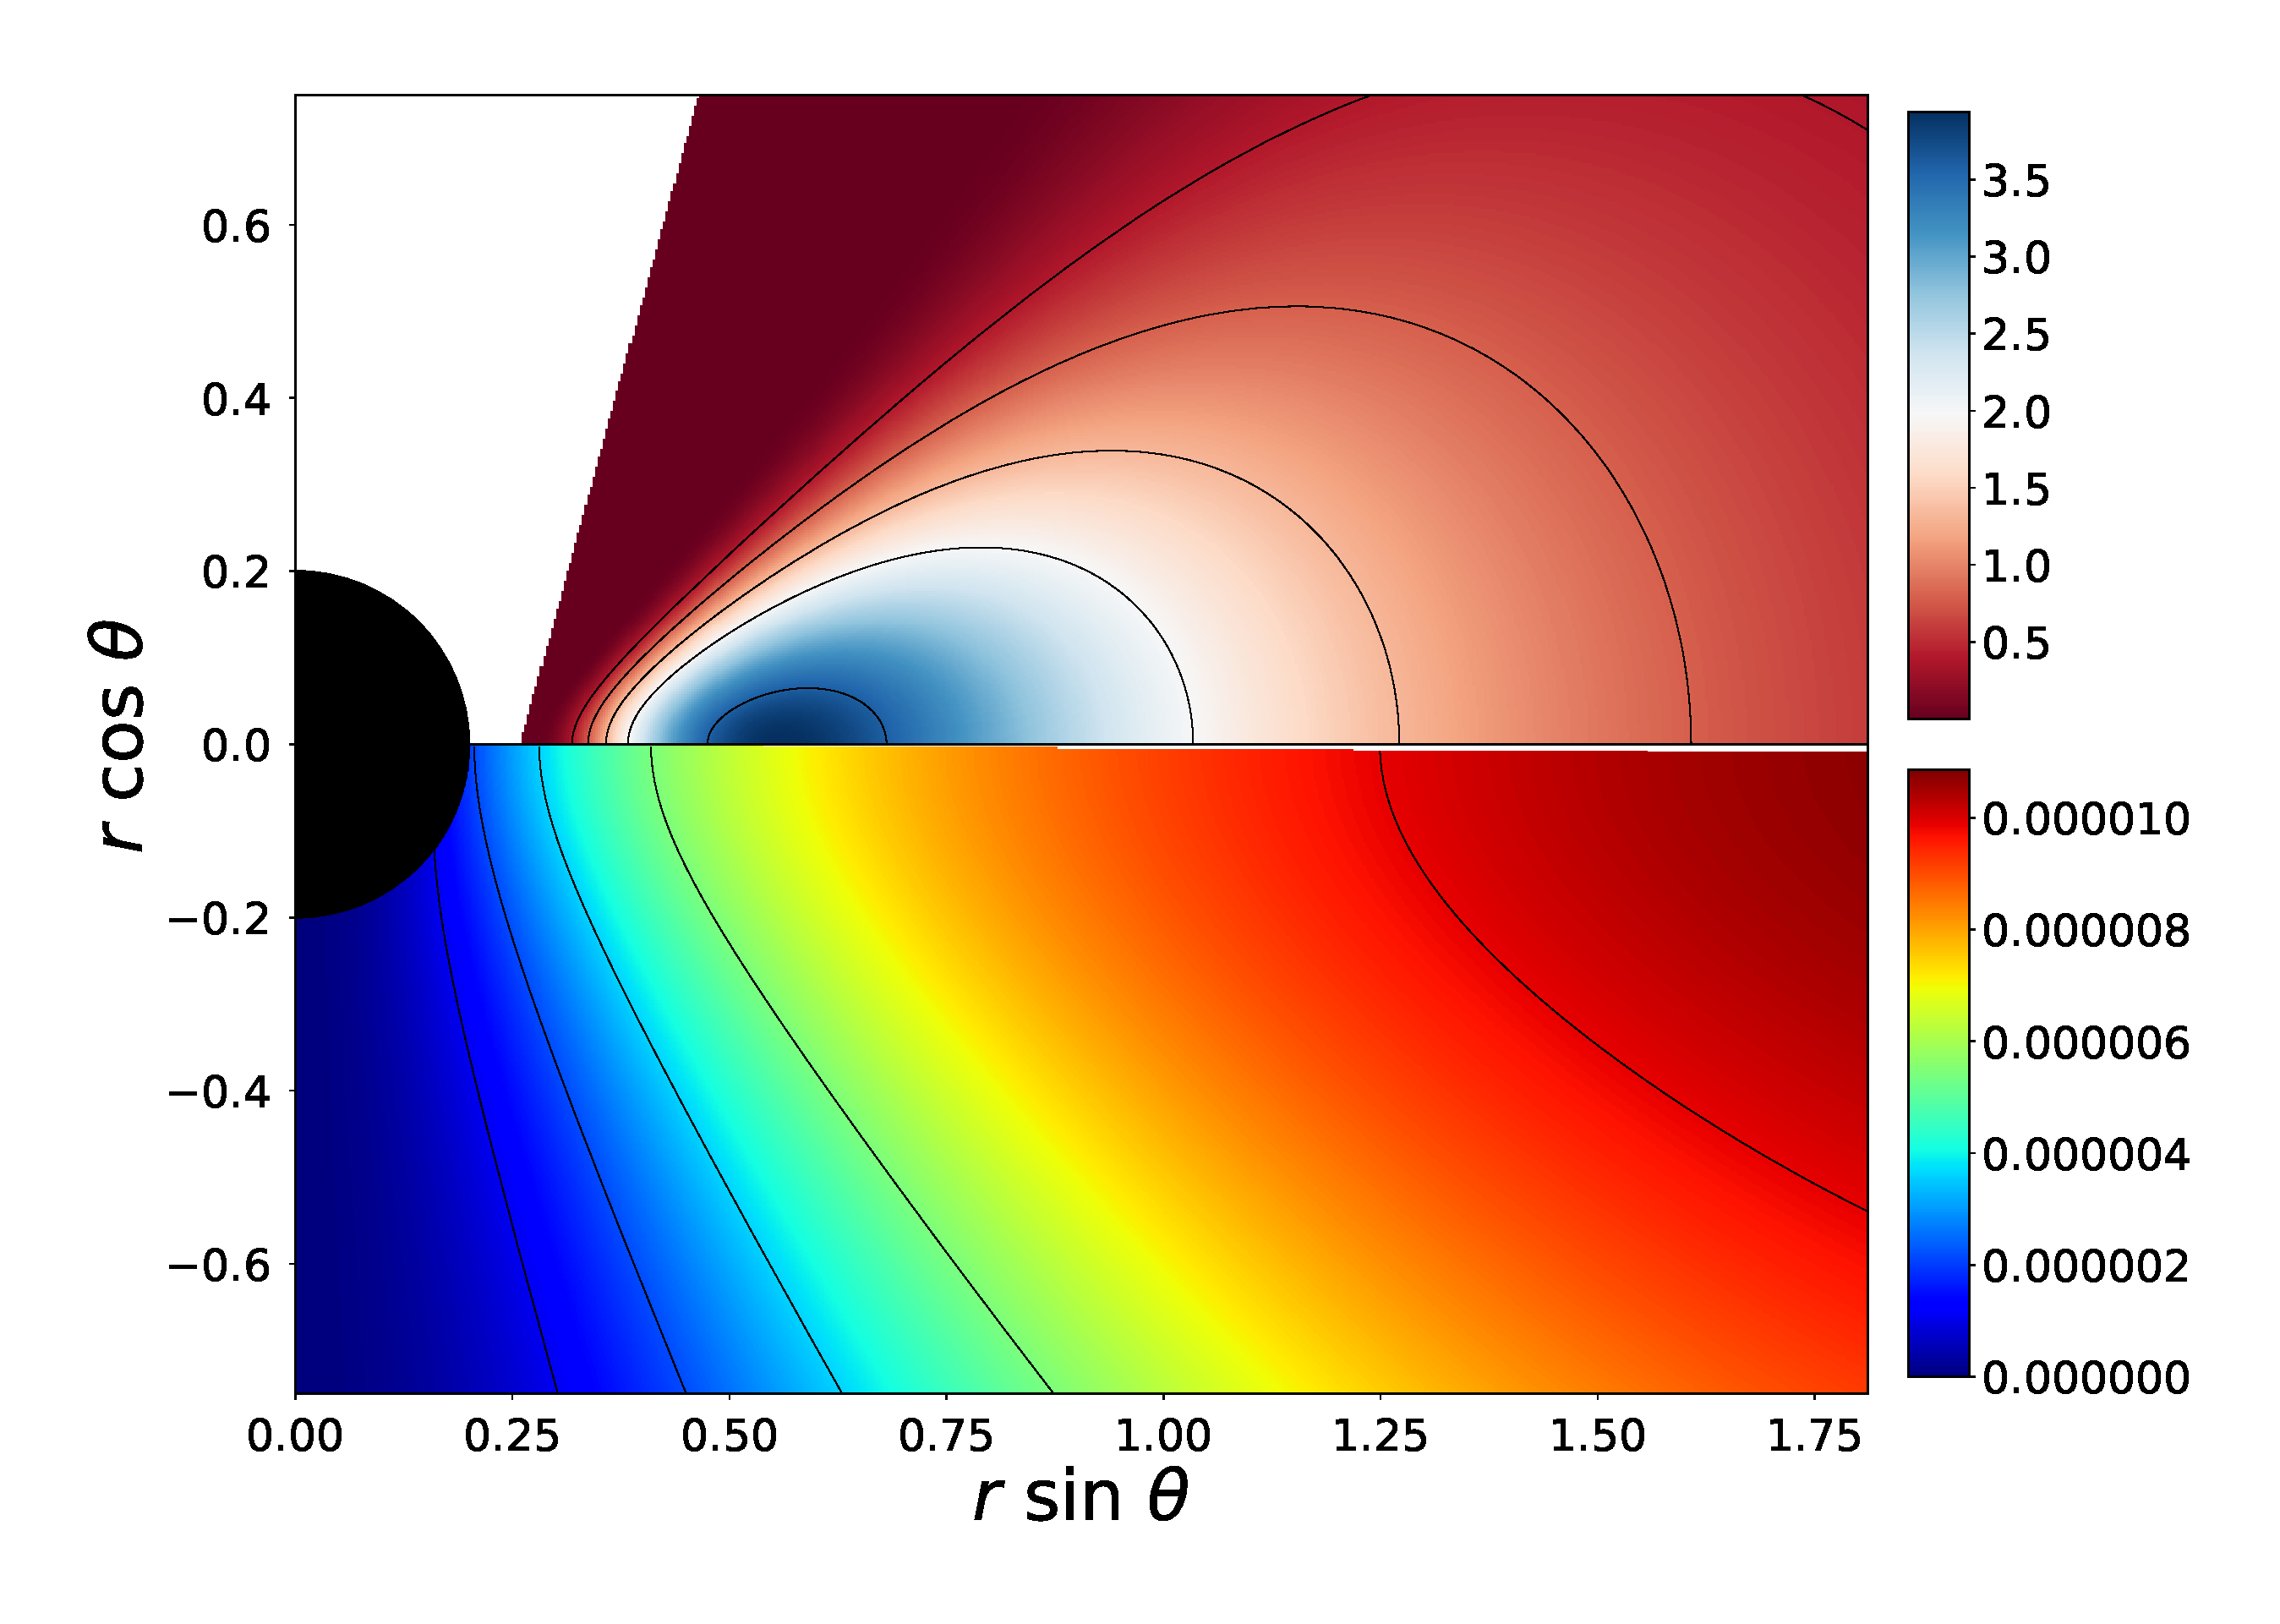
\includegraphics[scale=0.1267]{figures/fig5_I_10.pdf}
\hspace{-0.3cm}
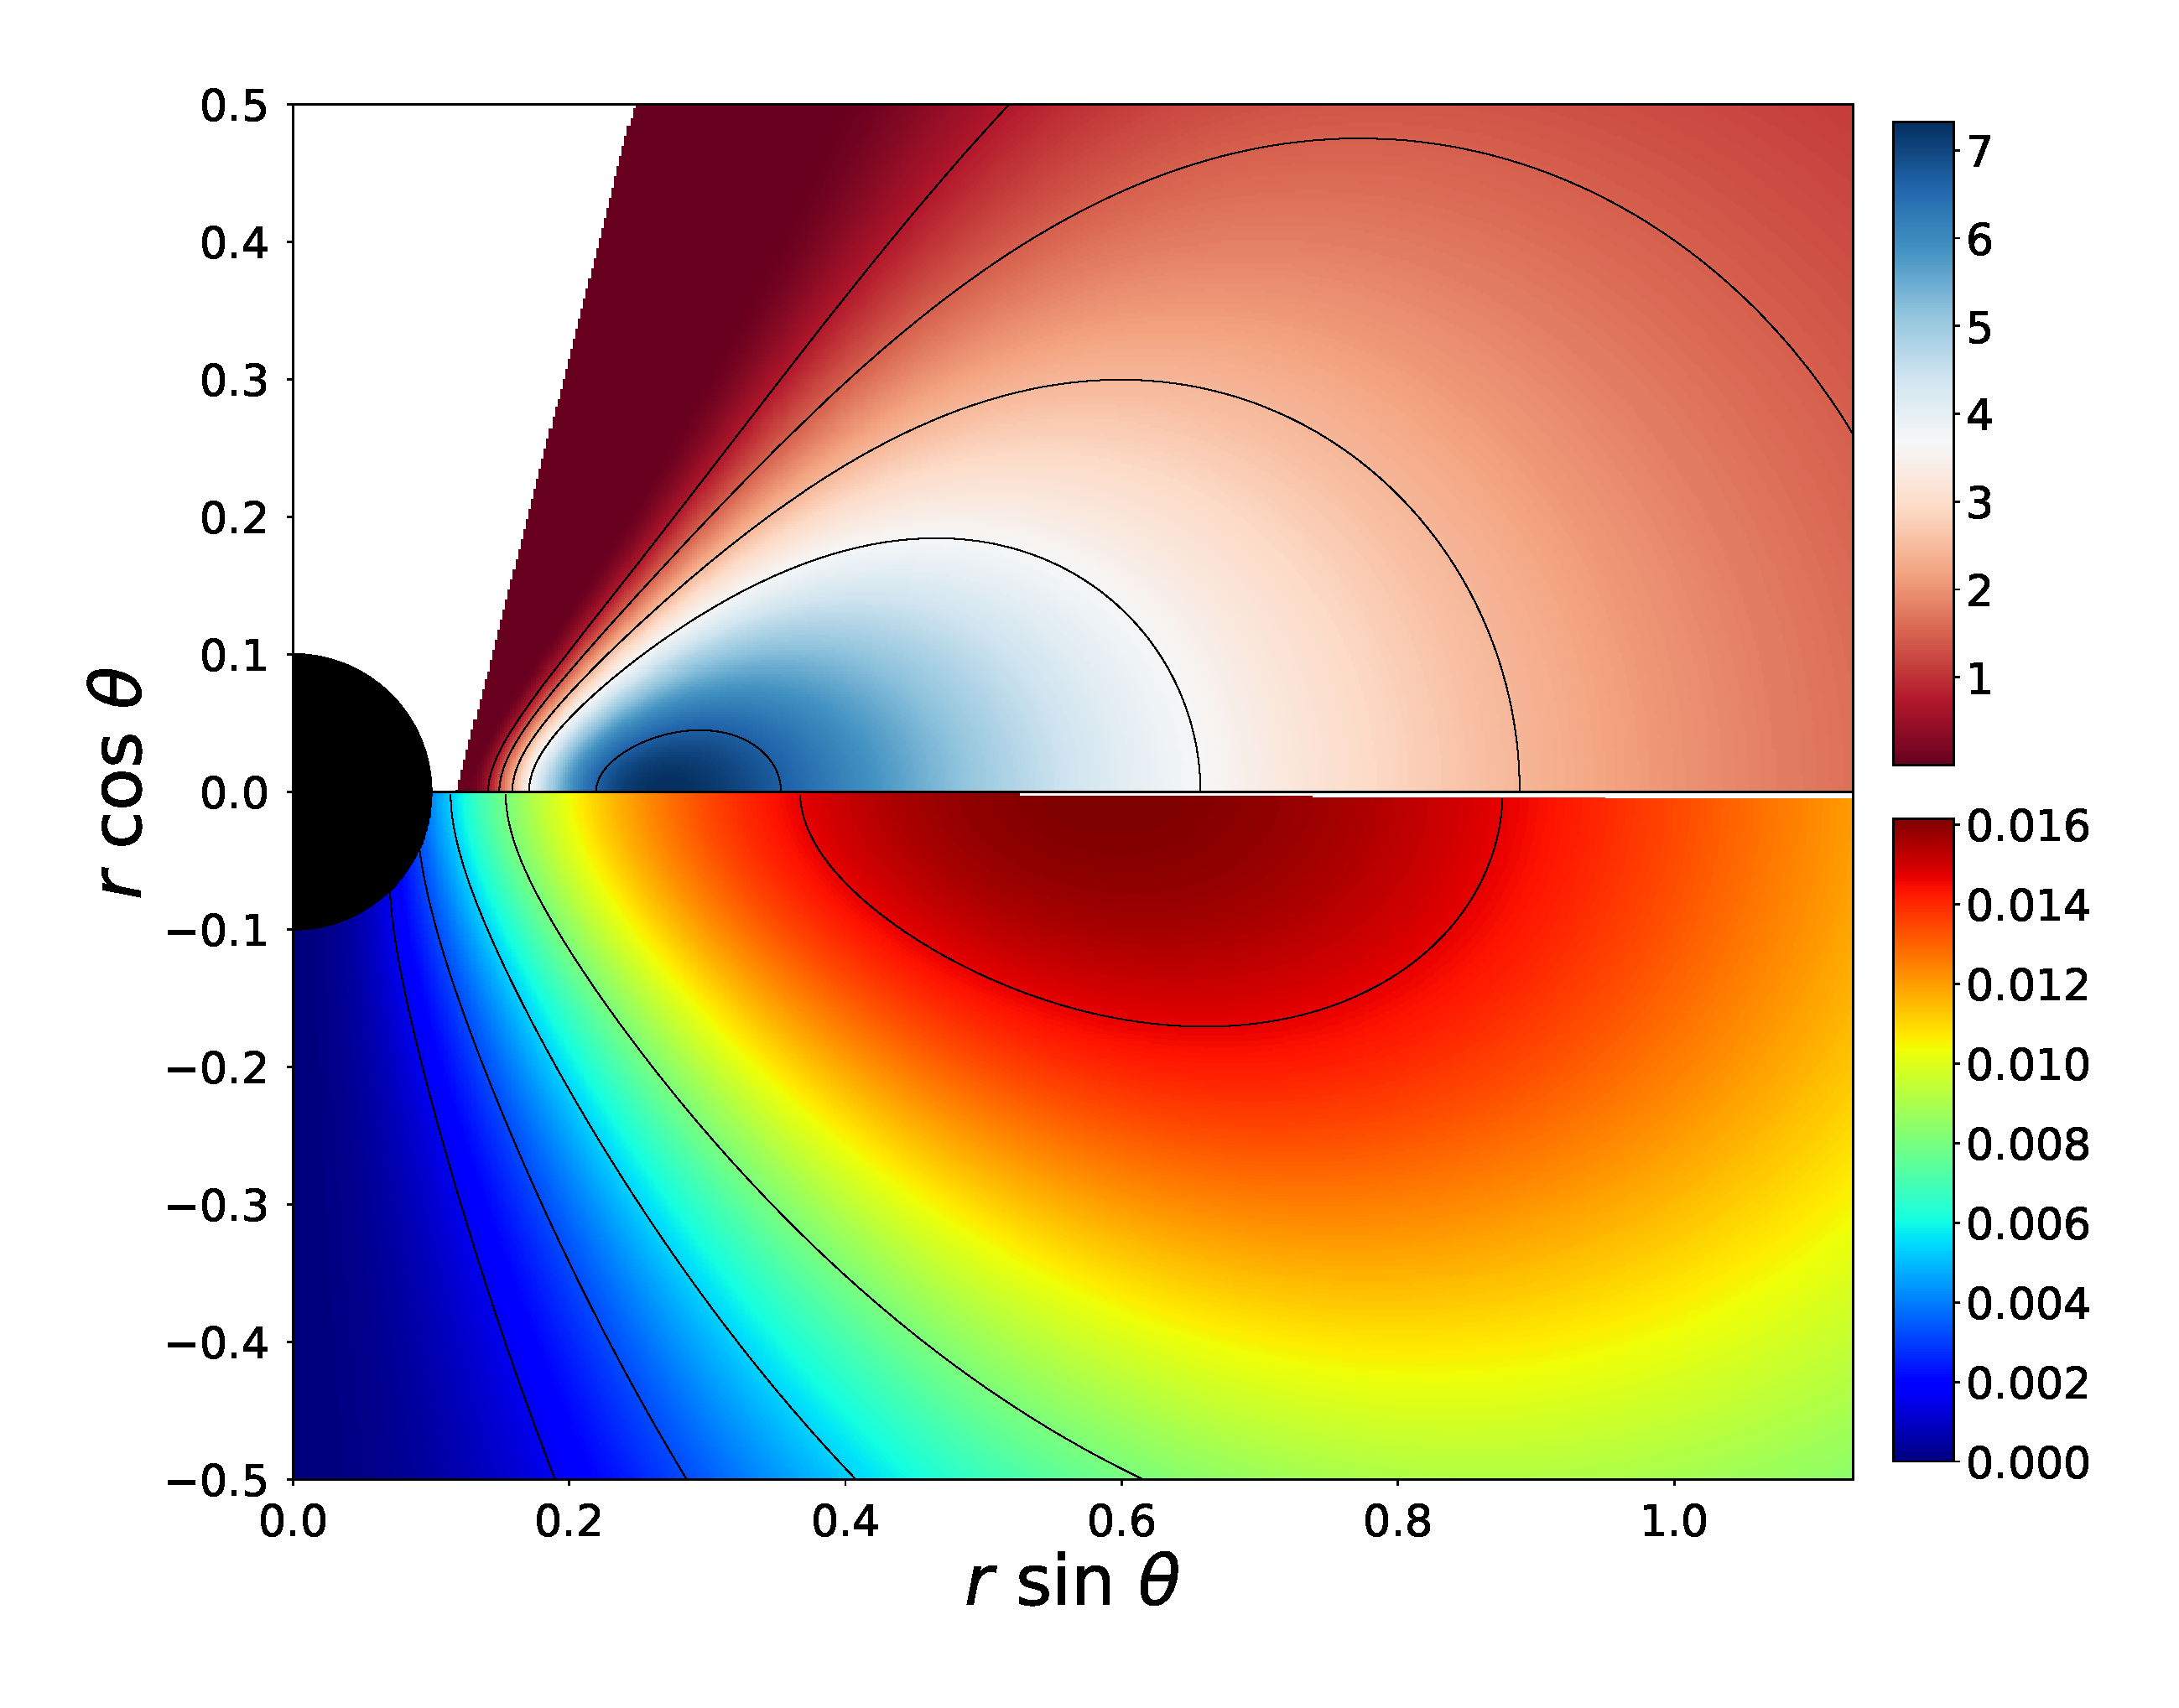
\includegraphics[scale=0.12]{figures/fig5_IV_10.pdf}
\hspace{-0.3cm}
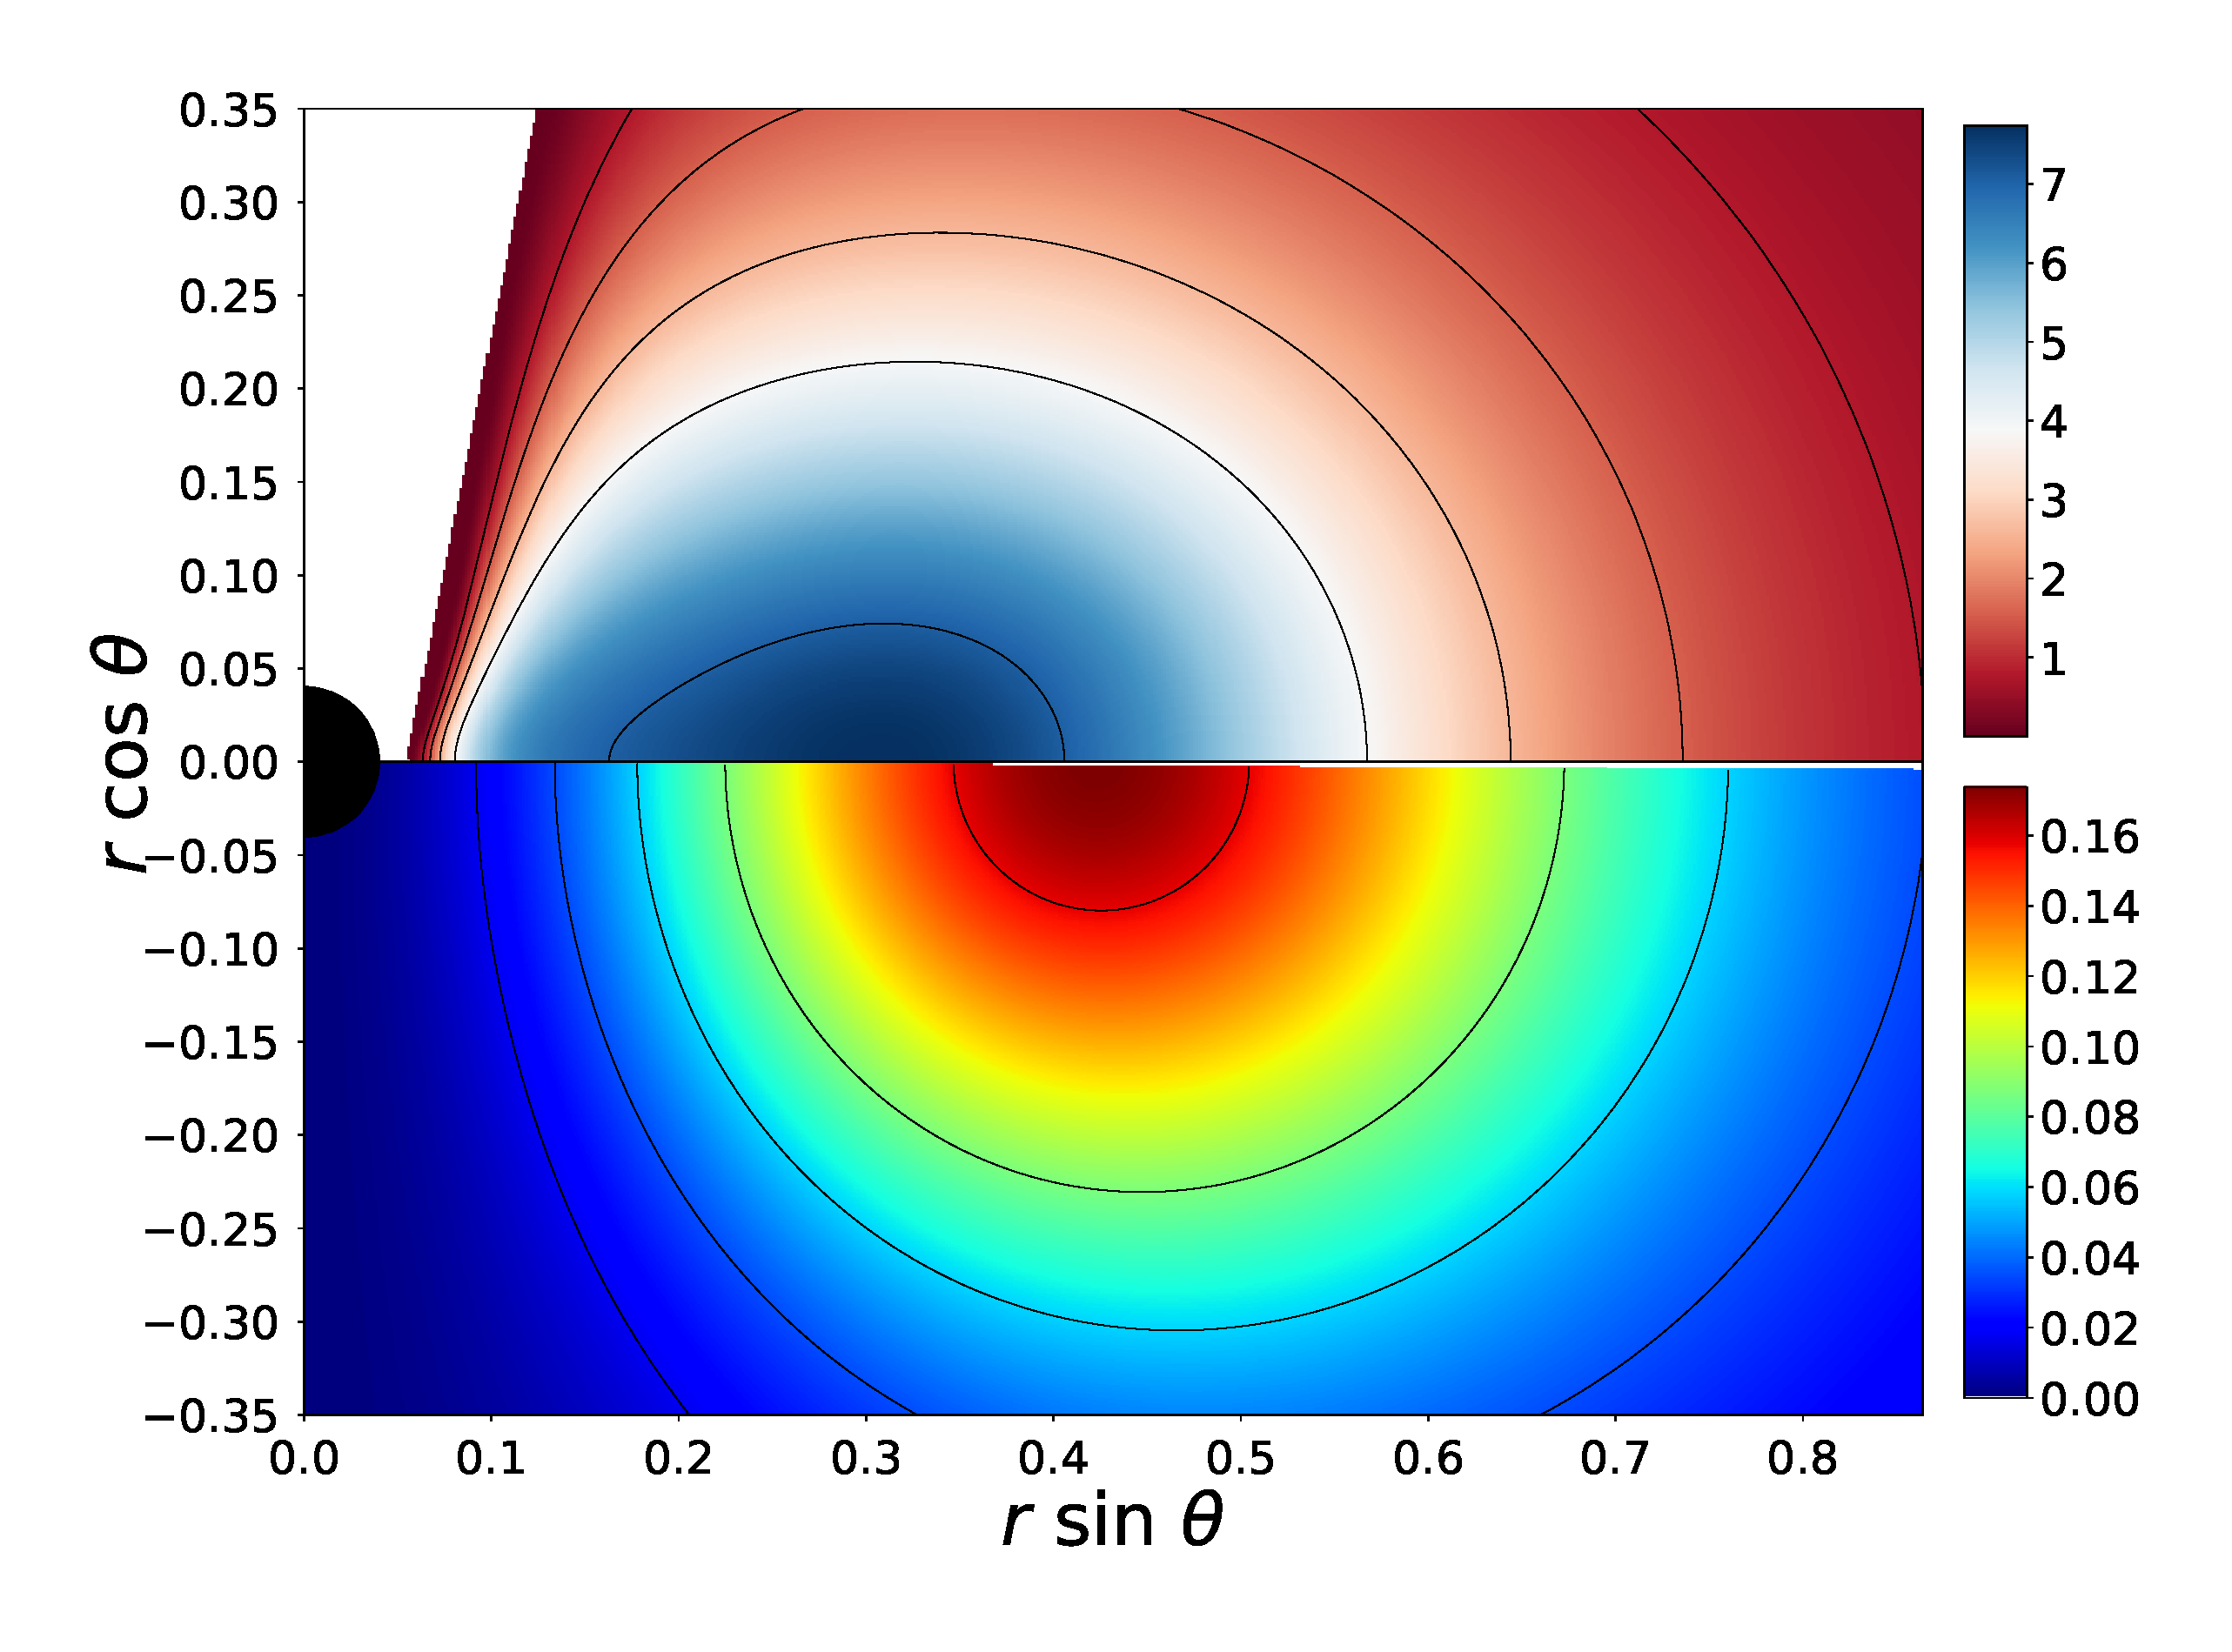
\includegraphics[scale=0.1267]{figures/fig5_VII_10.pdf}
\hspace{-0.2cm}
\\
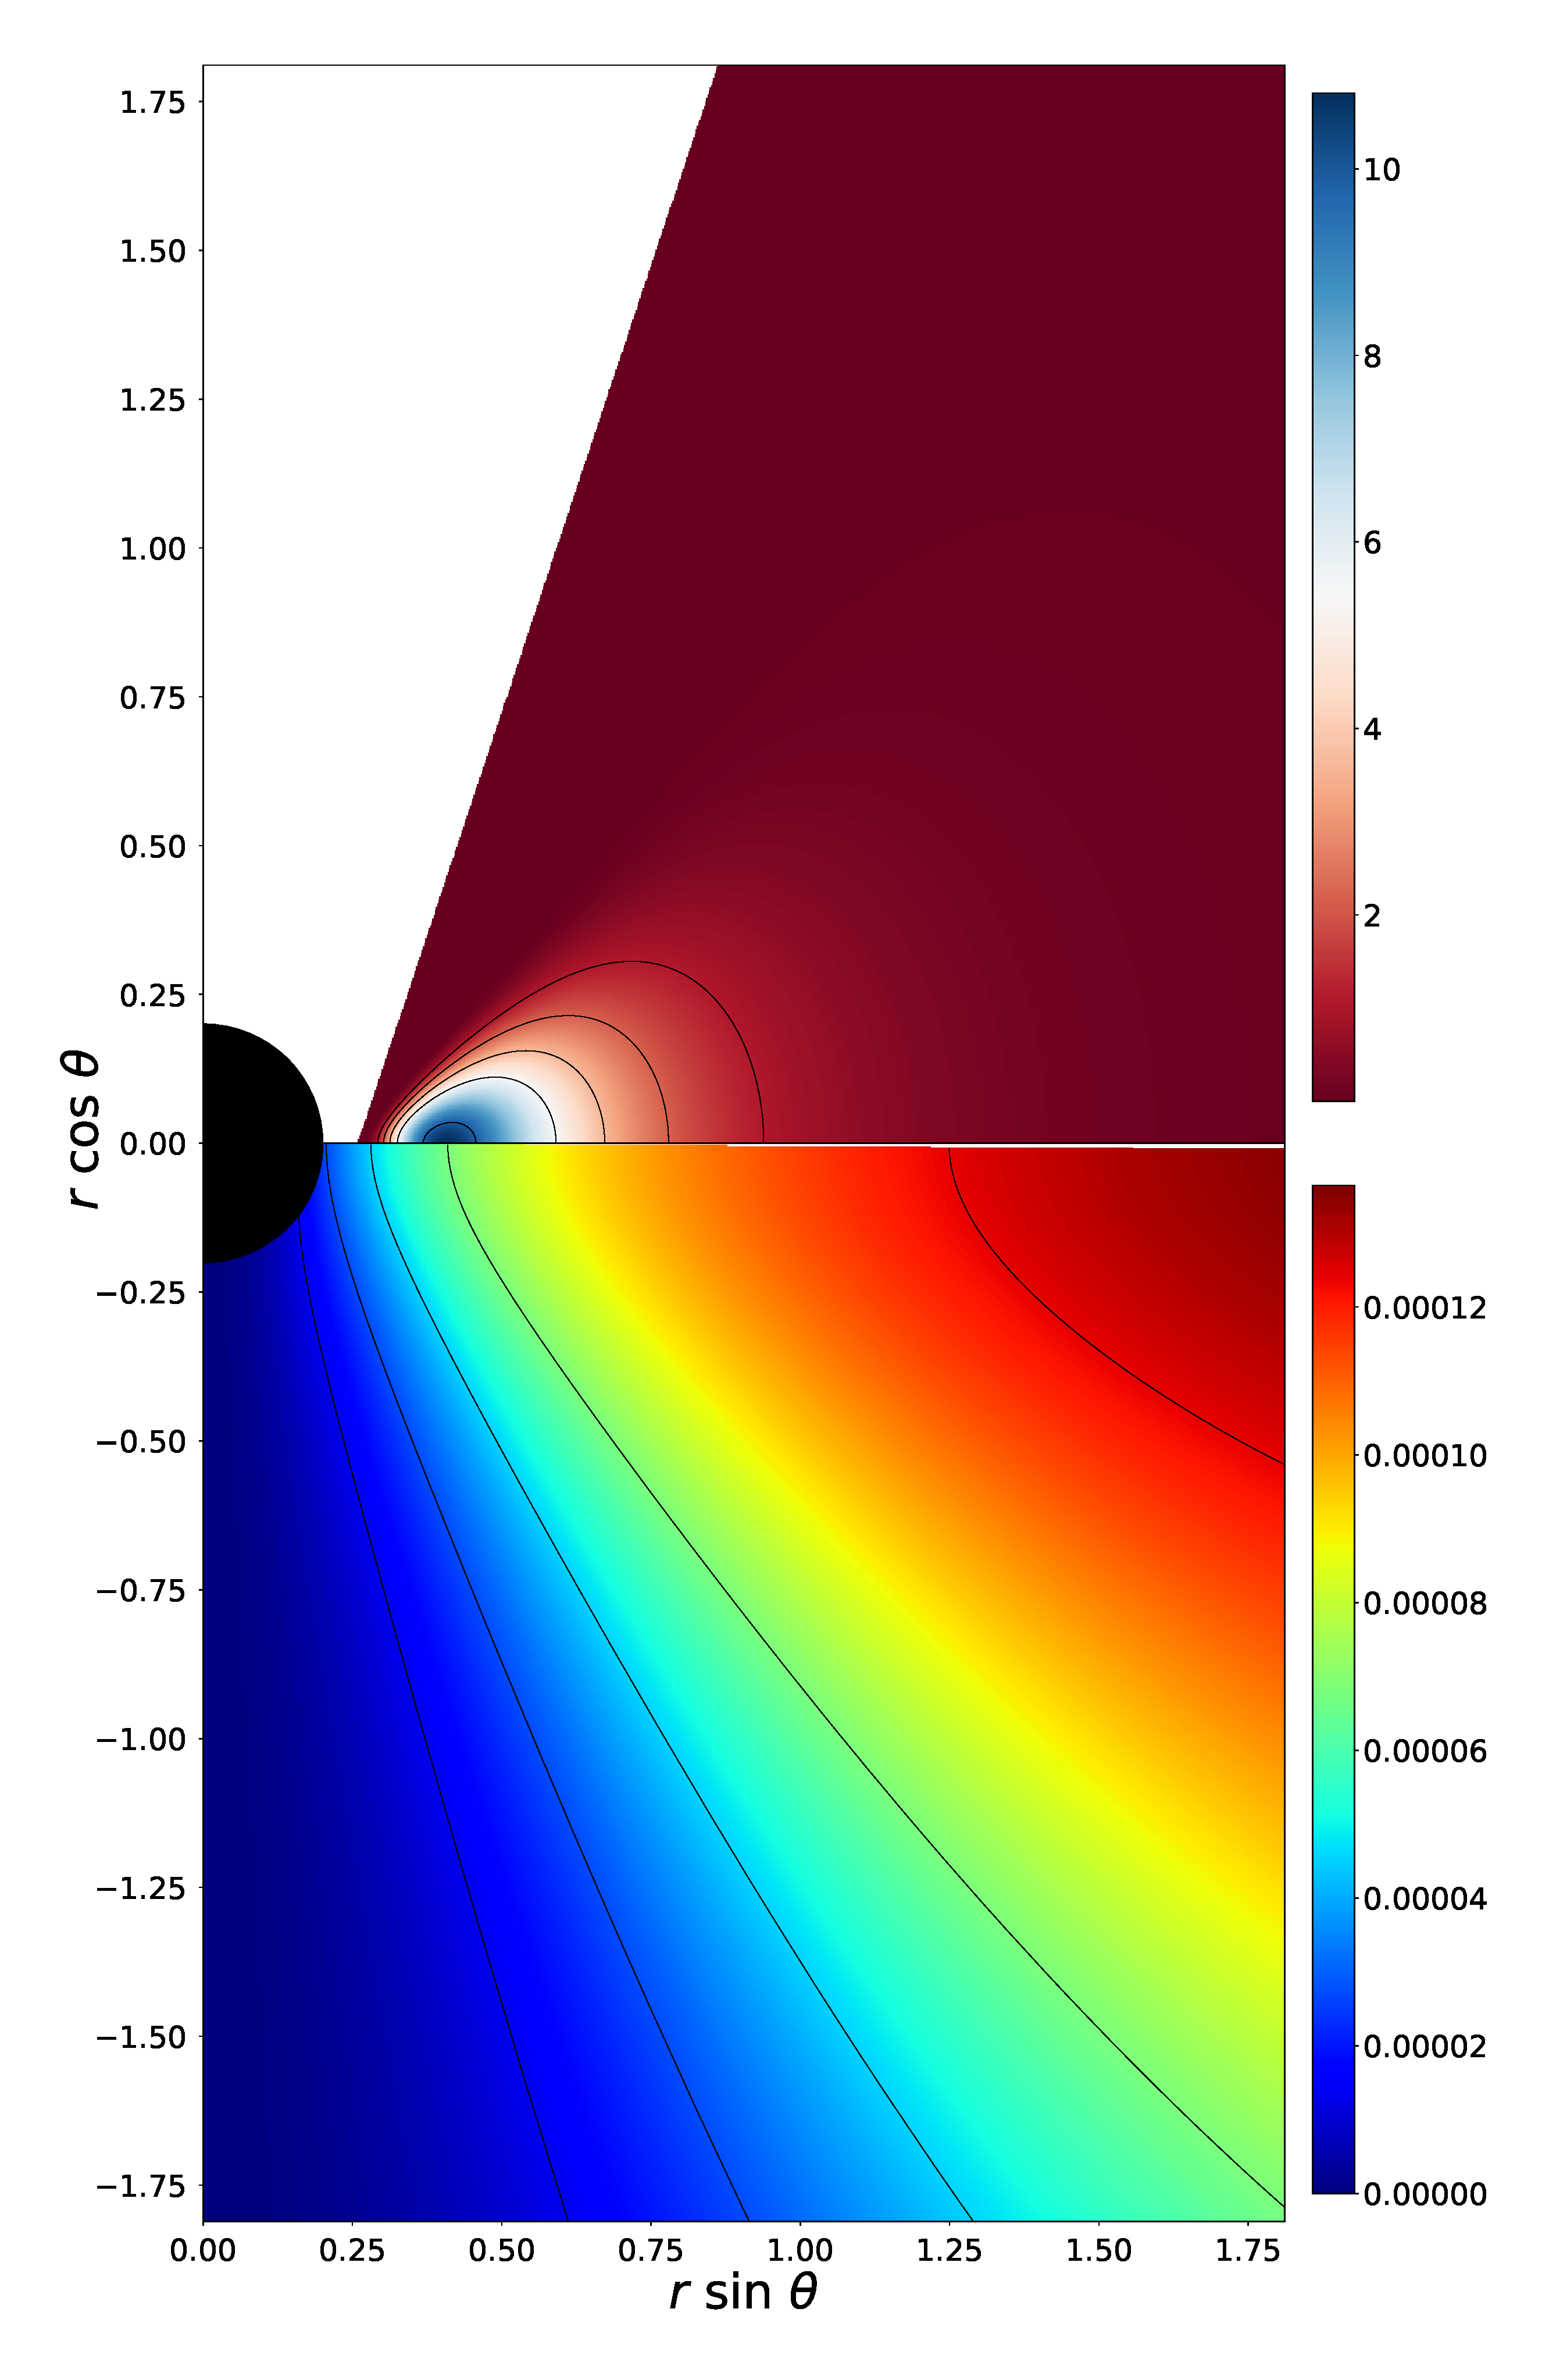
\includegraphics[scale=0.1267]{figures/fig5_I__10.pdf}
\hspace{-0.3cm}
\includegraphics[scale=0.12]{figures/fig5_IV__10.pdf}
\hspace{-0.3cm}
\includegraphics[scale=0.1267]{figures/fig5_VII__10.pdf}
\hspace{-0.2cm}
\caption{Energy density distribution for the torus $\rho_{\mathrm{T}}$ (upper half of the images) and for the scalar field $\rho_{\mathrm{SF}}$ (lower half). From left to right the columns correspond to models I, IV, and VII. The top row corresponds to non-magnetized models ($\beta_{\mathrm{m}_{\mathrm{c}}} = 10^{10}$) and the bottom row to strongly magnetized models ($\beta_{\mathrm{m}_{\mathrm{c}}} = 10^{-10}$).}
\label{comparison_mass_density}
\end{figure*}

The structure of the disks is similar for all values of $\beta_{\mathrm{m_c}}$ with the only quantitative differences being the location of the centre of the disk, which moves closer to the BH as the magnetization increases, and the range of variation of the isodensity contours, whose upper ends become larger with decreasing $\beta_{\mathrm{m_c}}$. This behaviour is in complete agreement with that found for KBHs in~\cite{Gimeno-Soler:2017} irrespective of the BH spin. For the particular case of Model VII, the maximum of the rest-mass density for the strongly magnetized case is significantly larger than for the other models and the spatial extent of the disk is significantly small. 

The size of the disks can be best quantified by plotting the radial profiles of the rest-mass density on the equatorial plane. This is shown in Fig.~\ref{radial_profiles_HBH} for models I, IV and VII and for the same three values of the magnetisation parameter shown in Figs.~\ref{models_I} and~\ref{models_II}. From this figure we see that model I disks are significantly larger than models IV and VII, i.e.~the hairier the models the more compact and smaller they become. We also note the presence of an extended region of high density in the unmagnetized model VII  (the mildly-magnetised case also shows this feature but to a lesser extent). This could be related to the existence of an extra gravitational well due to the scalar field distribution that overlaps with the matter distribution of the disk (as can be seen in the right panel of Fig.~\ref{comparison_mass_density} below).

In figures~\ref{models_peri_I} and~\ref{models_peri_II} we show the same morphological distribution of Figs.~\ref{models_I} and~\ref{models_II} but using, instead, a perimetral radial coordinate $R$, related to the radial coordinate $r$ according to $R = e^{F_2} r$. This perimetral coordinate represents the proper length along the azimuthal direction, which constitutes a geometrically meaningful direction since it runs along the orbits of the azimuthal Killing vector field. Therefore, the proper size of a full $\phi$ orbit is given by $2\pi R$, i.e.~$R$ is the perimetral radius. The most salient feature of the morphologies shown in Figs.~\ref{models_peri_I} and~\ref{models_peri_II}, when comparing to those displayed in Figs.~\ref{models_I} and~\ref{models_II}, is the deformation of the disks in their innermost regions. In general, the deformations become larger the higher the BH spin and the closer the disk is to the horizon. Model III is the one showing the largest deformation, as $R_{\rm in}-R_{\rm H}$ attains the smallest value for this model. \tf{Check.} It is also worth noticing that the shape of the BH also changes when using the perimetral coordinate. While in the $r$ coordinate the horizon is spherical (cf.~Figs.~\ref{models_I} and~\ref{models_II}) in the perimetral coordinate $R$ is not always so. Moreover, the larger the value of $v_{\rm H}$, the more elliptic the horizon becomes, which in our sample corresponds to model III. \tf{Check.}

\sg{Discuss. I find that the 2D morphology in perimeteral coordinates might not be very useful, but I found an interesting property of these coordinates: For the Kerr metric, $R_{\mathrm{H}} = 2M$ irrespective of the value of the angular momentum (For the KBHsSH cases, $2M_{\mathrm{H}} \neq R_{\mathrm{H}} \neq 2M_{\mathrm{ADM}}$. I don't know if there are any kind of dependence on the angular momentum, as we don't two cases with the same value of the mass). I suppose this could help us to compare different models. In fact, the differences in the morphology close to the equatorial plane in the near horizon region are actually related to the value of the angular momentum (we can see a relationship between the morphological differences and the equivalent spin parameter $a_{\mathrm{eq}}$).} \tf{Could you please include some of this information in here?}

Table~\ref{HBH_disk_parameters} reports the relevant physical quantities for all of our disk models around KBHsSH. It is worth mentioning that KBHsSH can violate the Kerr bound for the potential $\Delta W \equiv W_{\mathrm{in}} - W_{\mathrm{c}}$. As shown in~\cite{Abramowicz:1978}, constant angular momentum disks arround Kerr BHs exhibit a maximum for $|\Delta W|$ when the spin parameter $a\rightarrow 1$. This value is $\Delta W_{\mathrm{max}} = -\frac{1}{2} \ln 3 \simeq -0.549$. Models V, VI, and VII of our sample violate that bound. As a result, the maximum values of the fluid quantities for disks around KBHsSH are significantly larger than in the Kerr BH case. In both cases, these values increase as $|\Delta W|$ increases, irrespective of the magnetisation, as shown in Table~\ref{HBH_disk_parameters}.


%\begin{figure*}
%\centering
%\includegraphics[scale=0.12]{figures/fig6_I_10.pdf}
%\hspace{-0.4cm}
%\includegraphics[scale=0.12]{figures/fig6_IV_10.pdf}
%\hspace{-0.4cm}
%\includegraphics[scale=0.12]{figures/fig6_VII_10.pdf}
%\hspace{-0.2cm}
%\\
%\includegraphics[scale=0.12]{figures/fig6_I__10.pdf}
%\hspace{-0.4cm}
%\includegraphics[scale=0.12]{figures/fig6_IV__10.pdf}
%\hspace{-0.4cm}
%\includegraphics[scale=0.12]{figures/fig6_VII__10.pdf}
%\hspace{-0.2cm}
%\caption{Same as Fig.~\ref{comparison_mass_density} but using the perimetral radial coordinate. \tf{Same comment as in the previous figure regarding the vertical range, in this case $[-1.5,1.5]$ for all models.} \sg{Done}}
%\label{comparison_mass_density_peri}
%\end{figure*}


\begin{figure*}
\centering
\includegraphics[scale=0.14]{figures/fig9_0_10.pdf}
\hspace{-0.3cm}
\includegraphics[scale=0.14]{figures/fig9_0_1.pdf}
\hspace{-0.2cm}
\includegraphics[scale=0.14]{figures/fig9_0__10.pdf}
\\
\includegraphics[scale=0.14]{figures/fig9_05_10.pdf}
\hspace{-0.3cm}
\includegraphics[scale=0.14]{figures/fig9_05_1.pdf}
\hspace{-0.2cm}
\includegraphics[scale=0.14]{figures/fig9_05__10.pdf}
\\
\includegraphics[scale=0.14]{figures/fig9_09_10.pdf}
\hspace{-0.3cm}
\includegraphics[scale=0.14]{figures/fig9_09_1.pdf}
\hspace{-0.2cm}
\includegraphics[scale=0.14]{figures/fig9_09__10.pdf}
\\
\includegraphics[scale=0.14]{figures/fig9_09999_10.pdf}
\hspace{-0.3cm}
\includegraphics[scale=0.14]{figures/fig9_09999_1.pdf}
\hspace{-0.2cm}
\includegraphics[scale=0.14]{figures/fig9_09999__10.pdf}
\hspace{-0.2cm}
\caption{Rest-mass density distribution. From top to bottom the rows correspond to a sequence of KBHs with increasing spin parameter $a$ (0, 0.5, 0.9 and 0.9999). From left to right the columns correspond to different values of the magnetization parameter, namely non-magnetized ($\beta_{\mathrm{m}_{\mathrm{c}}} = 10^{10}$), mildly magnetized ($\beta_{\mathrm{m}_{\mathrm{c}}} = 1$) and strongly magnetized ($\beta_{\mathrm{m}_{\mathrm{c}}} = 10^{-10}$)}
\label{models_Kerr}
\end{figure*}

\begin{figure*}
\centering
\includegraphics[scale=0.14]{figures/fig10_0_10.pdf}
\hspace{-0.3cm}
\includegraphics[scale=0.14]{figures/fig10_0_1.pdf}
\hspace{-0.2cm}
\includegraphics[scale=0.14]{figures/fig10_0__10.pdf}
\\
\includegraphics[scale=0.14]{figures/fig10_05_10.pdf}
\hspace{-0.3cm}
\includegraphics[scale=0.14]{figures/fig10_05_1.pdf}
\hspace{-0.2cm}
\includegraphics[scale=0.14]{figures/fig10_05__10.pdf}
\\
\includegraphics[scale=0.14]{figures/fig10_09_10.pdf}
\hspace{-0.3cm}
\includegraphics[scale=0.14]{figures/fig10_09_1.pdf}
\hspace{-0.2cm}
\includegraphics[scale=0.14]{figures/fig10_09__10.pdf}
\\
\includegraphics[scale=0.14]{figures/fig10_09999_10.pdf}
\hspace{-0.3cm}
\includegraphics[scale=0.14]{figures/fig10_09999_1.pdf}
\hspace{-0.2cm}
\includegraphics[scale=0.14]{figures/fig10_09999__10.pdf}
\hspace{-0.2cm}
\caption{Rest-mass density distribution using perimeteral coordinates. From top to bottom the rows correspond to a sequence of KBHs with increasing spin parameter $a$ (0, 0.5, 0.9 and 0.9999). From left to right the columns correspond to different values of the magnetization parameter, namely non-magnetized ($\beta_{\mathrm{m}_{\mathrm{c}}} = 10^{10}$), mildly magnetized ($\beta_{\mathrm{m}_{\mathrm{c}}} = 1$) and strongly magnetized ($\beta_{\mathrm{m}_{\mathrm{c}}} = 10^{-10}$)}
\label{models_Kerr_peri}
\end{figure*}

\begin{figure*}
\centering
\includegraphics[scale=0.2]{figures/fig7_HBH_dens.eps}
\hspace{-0.cm}
\includegraphics[scale=0.2]{figures/fig7_HBH_enth.eps}
\hspace{-0.cm}
\\
\includegraphics[scale=0.2]{figures/fig7_Kerr_dens.eps}
\hspace{-0.cm}
\includegraphics[scale=0.2]{figures/fig7_Kerr_enth.eps}
\hspace{-0.cm}
\caption{Effects of the magnetization on the values for the maximum density (left) and enthalpy (right) of the disks. In the first row, we show this for all of our KBHsSH models. In the second row, we show this for a sequence of Kerr BHs with increasing spin parameter. \tf{Using yellow is a bad choice as it cannot be seen, especially on print. Please change the colour of the yellow dots to some other colour or symbol.}}
\label{comparison_HBH_Kerr_dens_enth}
\end{figure*}

\begin{figure*}
\centering
\includegraphics[width=0.4\textwidth]{figures/fig8_HBH.eps}
\hspace{0.5cm}
\includegraphics[width=0.4\textwidth]{figures/fig8_Kerr.eps}
\hspace{0.5cm}
\caption{Effects of the magnetization on the perimeteral location of the magnetic pressure maximum (divided by the the perimeteral radius of the centre), $R_{\mathrm{mag}, \mathrm{max}} - R_{\mathrm{c}})/ R_{\mathrm{c}}$). Left panel: KBHsSH models. Right panel: A sequence of KBHs with increasing spin parameter. \tf{Change the $r$ to $R$ in the vertical labels.}}
\label{comparison_HBH_Kerr_r_m_max}
\end{figure*}


\begin{table*}[t]
\caption{Disc parameters and values of their relevant physical magnitudes for the KBH case. For all the cases, we have $R_{\mathrm{in}} = R_{\mathrm{mb}}$ , $l = l_{\mathrm{mb}}$ and $M_{\mathrm{BH}} = 1$.}        
\label{KBH_disk_parameters}      
\centering          
\begin{tabular}{c c c c c  c c c c c c c}
\hline\hline       
 $a$ & $l$ & $W_{\mathrm{c}}$ & $R_{\mathrm{in}}$ & $R_{\mathrm{c}}$ &  $\beta_{\mathrm{m_{\mathrm{c}}}}$ & $h_{\mathrm{max}}$ & $\rho_{\mathrm{max}}$ & $p_{\mathrm{max}}$ & $p_{\mathrm{m, max}}$ & $R_{\mathrm{max}}$ & $R_{\mathrm{m, max}}$\\ 
\hline           
$0$ & $4.00$ & $-4.32 \times 10^{-2}$ & $4.00$ & $10.47$ & $10^{10}$ & $1.04$ & $1.0$ & $1.10 \times 10^{-2}$ & $1.15 \times 10^{-12}$ & $10.47$ & $11.86$\\ 
 \hline 
 &  &  &  &  & $1$ & $1.02$ & $1.11$ & $6.29 \times 10^{-3}$ & $5.69 \times 10^{-3}$ & $8.81$ & $9.52$\\ 
 \hline 
 &  &  &  &  & $10^{-10}$ & $1.0$ & $1.48$ & $1.83 \times 10^{-12}$ & $1.48 \times 10^{-2}$ & $7.70$ & $8.14$\\ 
 \hline 
 $0.5$ & $3.41$ & $-6.35 \times 10^{-2}$ & $2.99$ & $7.12$ & $10^{10}$ & $1.07$ & $1.0$ & $1.64 \times 10^{-2}$ & $1.72 \times 10^{-12}$ & $7.19$ & $8.14$\\ 
 \hline 
 &  &  &  &  & $1$ & $1.03$ & $1.12$ & $9.43 \times 10^{-3}$ & $8.47 \times 10^{-3}$ & $6.05$ & $6.53$ \\ 
 \hline 
 &  &  &  &  & $10^{-10}$ & $1.0$ & $1.53$ & $2.81 \times 10^{-12}$ & $2.23 \times 10^{-2}$ & $5.29$ & $5.59$\\ 
\hline  
$0.9$ & $2.63$ & $-0.129$ & $2.18$ & $3.78$ & $10^{10}$ & $1.14$ & $1.0$ & $1.64 \times 10^{-2}$ & $3.65 \times 10^{-12}$ & $3.78$ & $4.23$\\ 
 \hline 
 &  &  &  &  & $1$ & $1.07$ & $1.14$ & $2.03 \times 10^{-2}$ & $1.78 \times 10^{-2}$ & $3.25$ & $3.47$\\ 
 \hline 
 &  &  &  &  & $10^{-10}$ & $1.0$ & $1.70$ & $6.54 \times 10^{-12}$ & $4.92 \times 10^{-2}$ & $2.92$ & $3.04$ \\ 
 \hline 
$0.9999$ & $2.02$ & $-0.429$ & $2.00015$ & $2.034$ & $10^{10}$ & $1.54$ & $1.0$ & $0.134$ & $1.61 \times 10^{-11}$ & $2.034$ & $2.094$ \\ 
\hline 
 &  &  &  &  & $1$ & $1.29$ & $1.51$ & $0.110$ & $7.52 \times 10^{-2}$ & $2.0075$ & $2.014$\\ 
\hline 
 &  &  &  &  & $10^{-10}$ & $1.0$ & $6.17$ & $1.22 \times 10^{-10}$ & $0.491$ & $2.0021$ & $2.0030$ \\ 
\hline   
\end{tabular}
\end{table*}


\begin{table}
\caption{Angular velocity at the centre for the different models computed. In the first column, we present the angular velocity at the disc centre for the different KBHsSH models. In the second column, we present the angular velocity at the disc centre for a KBH with the same ADM quantities.\sg{to fill with the Kerr case values.}}
\label{angular_velocity_table}      
\centering          
\begin{tabular}{c c c }
\hline\hline       
 Model & $\Omega_{\mathrm{c}}$ & $\Omega_{\mathrm{ADM_c}}$ \\ 
\hline           
I & $0.493$ & $-$ \\ 
 \hline 
II & $0.424$ & $--$ \\
 \hline 
III & $0.521$ & $-$ \\ 
 \hline 
IV & $0.427$ & $-$ \\ 
 \hline 
V & $0.394$ & $-$ \\ 
 \hline 
VI & $0.350$ & $-$ \\ 
 \hline 
VII & $0.330$ & $-$ \\ 
\hline      
\end{tabular}
\end{table}

\begin{table}
\caption{Central density of the disc for the different models, considering a disc with a value of $r_{\mathrm{in}}$ such as $\Delta W = 0.9 \Delta W_{\mathrm{Total} \equiv W_{\mathrm{cusp}} - W_{\mathrm{c}}}$ and a torus gravitational mass of $M_{\mathrm{T}} = 0.1 M_{\mathrm{ADM}}$. In the first column, we present the value of the central density for the different KBHsSH models. In the second column, we present the central density for a KBH with the same ADM quantities.\sg{To fill with the Kerr case values.}}
\label{central_density_table}      
\centering          
\begin{tabular}{c c c c }
\hline\hline       
 Model & $\beta_{\mathrm{m_{\mathrm{c}}}}$ & $\rho_{\mathrm{c}}$ & $\rho_{\mathrm{ADM_c}}$ \\ 
\hline           
I & $10^{10}$ & $0.002051$ & $-$ \\ 
 \hline 
 & $1$ & $0.00434$ & $-$ \\ 
 \hline 
 & $10^{-10}$ & $0.00531$ & $-$ \\ 
 \hline 
II & $10^{10}$ & $0.00150$ & $-$ \\ 
 \hline 
 & $1$ & $0.00427$ & $-$ \\ 
 \hline 
 & $10^{-10}$ & $0.00582$ & $-$ \\ 
 \hline 
III & $10^{10}$ & $0.00304$ & $-$ \\ 
 \hline 
 & $1$ & $0.00840$ & $-$ \\ 
 \hline 
 & $10^{-10}$ & $0.0108$ & $-$ \\ 
 \hline 
IV & $10^{10}$ & $0.00407$ & $-$ \\ 
 \hline 
 & $1$ & $0.00897$ & $-$ \\ 
 \hline 
 & $10^{-10}$ & $0.0110$ & $-$ \\ 
 \hline 
V & $10^{10}$ & $0.00577$ & $-$ \\ 
 \hline 
 & $1$ & $0.0104$ & $-$ \\ 
 \hline 
 & $10^{-10}$ & $0.0121$ & $-$ \\ 
 \hline 
VI & $10^{10}$ & $0.00762$ & $-$ \\ 
 \hline 
 & $1$ & $0.0116$ & $-$ \\ 
 \hline 
 & $10^{-10}$ & $0.0131$ & $-$ \\ 
 \hline 
VII & $10^{10}$ & $0.0129$ & $-$ \\ 
 \hline 
 & $1$ & $0.0162$ & $-$ \\ 
 \hline 
 & $10^{-10}$ & $0.01701$ & $-$ \\ 
 \hline     
\end{tabular}
\end{table}

In figure~\ref{comparison_mass_density} we show the total energy density of the torus $\rho_{\mathrm{T}}$ (upper half of each image) and the total energy density of the scalar field $\rho_{\mathrm{SF}}$ (lower half) for models I, IV and VII and two  values of the magnetisation parameter at the center ($10^{10}$, top row, and $10^{-10}$, bottom row). This figure shows that, for non-magnetised disks, the maximum of the total energy density of the disk $\rho_{\mathrm{T}}$ is closer to the maximum of the total energy density of the scalar field $\rho_{\mathrm{SF}}$ for increasing hair. This trend disappears with increasing magnetisation, as the disk moves closer to the horizon in such case.

%%%%%%%%%%%%%%%%%%%%%
\subsection{Comparison with Kerr BHs}
%%%%%%%%%%%%%%%%%%%%%

For the sake of comparison we build equilibrium sequences of magnetised disks around four Kerr BHs of varying spins, from $a=0$ to $a=0.9999$. Our numerical approach can handle BH spins as large as $|a-1|=10^{-10}$ \tf{Check} but such extreme cases do not add further relevant information to our discussion. Table~\ref{KBH_disk_parameters} reports a summary of the main physical quantities of these disks, whose morphology is displayed in Figs.~\ref{models_Kerr} and~\ref{models_Kerr_peri}. As for the disks built around KBHsSH, the maximum values of the enthalpy, density, pressure and magnetic pressure increase with increasing $|\Delta W|$, which, in the Kerr BH case, also means with increasing values of $a$. It can be seen that both the cusp and the centre move closer to the horizon with increasing $a$. \tf{Describe further the table and the figures}. \tf{Mention that the horizon location is constant in perimetral coordinates irrespective of $a$.} 

Also, in figures~\ref{models_Kerr} and~\ref{models_Kerr_peri} we show different KBH models with the same mass $M_{\mathrm{BH}} = 1$ and different values for the spin parameter($0$, $0.5$, $0.9$, $0.9999$). 

\sg{Compare the radial profiles.}
\sg{Describe and compare the angular velocity at the centre.}


% As shown in~\cite{Delgado:2018} some \sg{(compute which ones are embeddable and which are not)} of our models are in the region of the domain of existence where the event horizon is not embeddable in $\mathbb{E}^3$ then, the shaded regions depicting the horizon that we show at several of the figures are not faithful representations of the horizon geometry. Nevertheless, we show them for the sake of clarity. Also, this led us to asking ourselves if this could also happen for the shape of the accretion tori and therefore, we should be conservative when extracting information about the morphology of the disks from 2-dimensional plots. This idea is discussed in appendix~\ref{torus_embedding}.

%%%%%%%%%%%%%%%%%%
\subsection{Magnetisation profiles}
%%%%%%%%%%%%%%%%%%

The dependence of the maximum specific enthalpy $h_{\mathrm{max}}$ and the maximum rest-mass density $\rho_{\mathrm{max}}$ with the magnetization parameter is shown in figures~\ref{comparison_HBH_Kerr_dens_enth}. The upper panels correspond to the KBHsSH models (I-VII) and the lower ones to our sequence of Kerr BHs with increasing spin parameter. For both cases, an increase in $|\Delta W|$ implies monotonically  higher values for $h_{\mathrm{max}}$ (low magnetisation) and also higher values for $\rho_{\mathrm{max}}$ (high magnetisation). However, there are quantitative differences between the two cases. For the enthalpy, the values of $h_{\mathrm{max}}$ reached for disks around KBHsSH are much higher than those of the Kerr BH case. This implies that, while the $w = \rho h \simeq \rho$ approximation (employed in~\cite{Komissarov:2006,Gimeno-Soler:2017}) is valid for magnetized disks ($\beta_{\mathrm{m_c}} \sim 1$) around Kerr BHs for values of the spin parameter as high as $a \sim 0.99$, that is not the case for disks around KBHsSH. We note that for the most extreme spin value we can build, $a=XXX$, the maximum enthalpy is $h_{\rm max}=XXX$. \tf{Complete.}
%Also, for the rest-mass density we have a different behaviour: $\rho_{\mathrm{max}}$ for KBHsSH reach values only attainable by high spin parameter KBHs (between $a = 0.9$ and $a = 0.99999$ for the seven models we present here).

Figure~\ref{comparison_HBH_Kerr_r_m_max} shows the relative variation of the quotient of the perimetral radius of the magnetic pressure maximum and the perimetral radius of the disk center, $(R_{\mathrm{m, max}}-R_{\mathrm{c}})/R_{\mathrm{c}}$, with the decimal logarithm of the magnetization parameter at the center of the disk, $\log_{10} \beta_{\mathrm{m_c}}$. The curves plotted correspond to the same KBHsSH and Kerr BH cases as those in figure~\ref{comparison_HBH_Kerr_dens_enth}. For all cases, the radial location of the magnetic pressure maximum decreases with decreasing $\beta_{\mathrm{m_c}}$. In~\cite{Gimeno-Soler:2017} we proved that for $h=1$ disk models in stationary and axisymmetric BH spacetimes, the location of the maximum of the magnetic pressure is identical for all models when $\beta_{\mathrm{m_c}}\equiv 1 / \Gamma - 1=3$. This condition is also fulfilled for the Kerr BH case  even when $h \neq 1$, with a slight deviation for cases with very high spin parameter, as can be seen in the inset of the right panel of Fig.~\ref{comparison_HBH_Kerr_r_m_max}. However, this condition is not fulfilled for disks built around KBHsSH (see inset in the left panel). At this point, it is relevant to remember that some of the KBHsSH models violate the Kerr bound in terms of the potential. As we mentioned previously, we need a small value of $\Delta W$ for the $h \simeq 1$ approximation to be valid in the non-magnetised regime. Now we can see that, in the KBHsSH case, this approximation is not valid even for mildly-magnetised discs.

%%%%%%%%%%%%%%%%%%
\subsection{Torus mass}
%%%%%%%%%%%%%%%%%%

\sg{Even the models we have computed are non-self gravitating, for the sake of astrophysical relevance, we computed the mass of some of the discs. For this case only, we have dropped the $\rho_{\mathrm{c}} = 1$ choice and instead, we have chosen that the mass of the torus must be $M_{\mathrm{T}} = 0.1 M_{\mathrm{ADM}}$. This is in agreement with the torus masses found as the final state of binary neutron stars mergers}

\sg{I think here we should go further and do the following: First, choose a suitable maximum ADM mass for the KBHsSH (Eq~(I.1) of~\cite{Herdeiro:2016}), this implies a choice of scalar field mass $\mu$. This maximum mass should be such as our models ADM mass would be $\sim 2.5 M_{\odot}$. Next, we should compute the central density for the models we want to compare (models I, IV, VII for 3 magnetisations and their Kerr ADM equivalents). Finally, we compute the cgs central densities with the formula (From the book of Rezzolla \emph{Relativistic Hydrodynamics})}
\begin{equation}
\rho_{\mathrm{cgs}} = 6.17714 \times 10^{17} \left(\frac{G}{c^2}\right)\left(\frac{M_{\odot}}{M}\right)^2 \rho_{\mathrm{geo}}
\end{equation}
\sg{and compare the central densities (or maximum) with known values.}


%\begin{table}
%\caption{List of models of KBHsSH.}        
%\label{models_list}      
%\centering          
%\begin{tabular}{c c c c  c c c c}
%\hline\hline       
% Model & $M_{\mathrm{ADM}}$ & $J_{\mathrm{ADM}}$ & $M_{\mathrm{H}}$ &  $J_{\mathrm{H}}$ & $M_{\mathrm{SF}}$ & $J_{\mathrm{SF}}$ & $r_{\mathrm{H}}$ \\ 
%\hline           
%I & $0.415$ & $0.172$ & $0.393$ &  $0.15$  & $0.022$ & $0.022$ & $0.2$\\ 
% \hline 
%II & $0.630$ & $0.403$ & $0.340$ &  $0.121$  & $0.063$ & $0.282$ & $0.221$ \\
% \hline 
%III & $0.797$ & $0.573$ & $0.365$ &  $0.172$  & $0.573$ & $0.432$ & $0.111$ \\ 
% \hline 
%IV & $0.933$ & $0.739$ & $0.234$ &  $0.114$  & $0.699$ & $0.625$ & $0.1$ \\ 
% \hline 
%V & $0.940$ & $0.757$ & $0.159$ &  $0.076$  & $0.757$ & $0.781$ & $0.091$ \\ 
% \hline 
%VI & $0.959$ & $0.795$ & $0.087$ &  $0.034$  & $0.872$ & $0.781$ & $0.088$ \\ 
% \hline 
%VII & $0.975$ & $0.85$ & $0.018$ &  $0.002$  & $0.957$ & $0.848$ & $0.04$ \\ 
%\hline      
%\end{tabular}
%\end{table}
%
%\begin{table}
%\caption{Values of the normalized spin parameter for the ADM quantities ($a_{\mathrm{ADM}}$), for the BH horizon quantities ($a_{\mathrm{H}}$), the horizon linear velocity ($v_{\mathrm{H}}$) and the spin parameter corresponding to a KBH with a linear velocity equal to $v_{\mathrm{H}}$, ($a_{\mathrm{H_{eq}}}$).}        
%\label{models_spin_vel}      
%\centering          
%\begin{tabular}{c c c c c}
%\hline\hline       
% Model & $a_{\mathrm{ADM}}$ & $a_{\mathrm{H}}$ & $v_{\mathrm{H}}$ & $a_{\mathrm{H_{eq}}}$ \\ 
%\hline           
%I & $0.9987$ & $0.9712$ & $0.7685$ & $0.9663$ \\ 
% \hline 
%II & $1.014$ & $0.3760$ & $0.6802$ & $0.9301$ \\
% \hline 
%III & $0.9032$ & $1.295$ & $0.7524$ & $0.9608$ \\ 
% \hline 
%IV & $0.8489$ & $2.082$ & $0.5635$ & $0.8554$ \\ 
% \hline 
%V & $0.8560$ & $3.017$ & $0.4438$ & $0.7415$ \\ 
% \hline 
%VI & $0.9477$ & $3.947$ & $0.2988$ & $0.5487$ \\ 
% \hline 
%VII & $0.8941$ & $6.173$ & $0.09732$ & $0.1928$ \\ 
%\hline      
%\end{tabular}
%\end{table}


%%%%%%%%%%%%
\section{Conclusions}
\label{conclusions}
%%%%%%%%%%%%

Future work: Non-constant angular momentum case, Proca hair, shadows of the system HBH+disk.

\begin{acknowledgements}

\end{acknowledgements}

\bibliographystyle{apsrev4-1}
\bibliography{references.bib}

\begin{appendix}
% \section{Embedding of the accretion torus in $\mathbb{E}^3$}\label{torus_embedding}
% Following the same reasoning as in~\cite{Delgado:2018}, we write the 2-metric for the surface of a torus as 
% \begin{equation}\label{eq:torus_prev_metric}
% \mathrm{d}\sigma^2 = \frac{e^{2 F_1}}{N}\mathrm{d}r^2+ e^{2 F_1}r^2\mathrm{d}\theta^2+e^{2 F_2} r^2 \sin^2\theta \mathrm{d}\phi^2,
% \end{equation}
% and the condition $r = r(\theta)$ for the surface of the torus. The location of the surface of the torus $r(\theta)$ can be obtained integrating $r' = \frac{\mathrm{d}r}{\mathrm{d}\theta} = -\frac{\partial_{\theta}W}{\partial_{r}W}$ (equation (24) of~\citep{Gimeno-Soler:2017}). Using this, we can write equation~\eqref{eq:torus_prev_metric} as
% \begin{equation}\label{eq:torus_metric}
% \mathrm{d}\sigma^2 = e^{2 F_1} \mathrm{d}\theta^2\left(\frac{r'^2}{N} +r^2\right)+e^{2 F_2} r^2 \sin^2\theta \mathrm{d}\phi^2,
% \end{equation}
% with the prime $'$ denoting partial differentiation with respect to $\theta$. Then, we try the embedding in $\mathbb{E}^3$ with the Cartesian metric $\mathrm{d}\sigma^2 = \mathrm{d}X^2 + \mathrm{d}Y^2 + \mathrm{d}Z^2$ and the embedding functions:
% \begin{equation}
% X + \mathrm{i}Y = f(\theta)e^{\mathrm{i}\phi},  \;\;\; Z = g(\theta),
% \end{equation}
% then
% \begin{equation}
% f = e^{2 F_2} r^2 \sin^2\theta, \;\;\; f'^2 + g'^2 = e^{2 F_1}\left(\frac{r'^2}{N} +r^2\right),
% \end{equation}
% so we can write $g'^2$ as
% \begin{equation}\label{eq:embedding_existance}
% g'^2 = e^{2 F_1}\left(\frac{r'^2}{N} +r^2\right) - e^{2 F_2} (F_2'r \sin \theta + r' \sin \theta + r \cos \theta)^2.
% \end{equation}
% This result tells us that the r.h.s. of~\eqref{eq:embedding_existance} must be $\geq 0$ in order to the embedding function to exist.

% \begin{figure*}
% \centering
% \includegraphics[scale=0.2]{figures/embedding.pdf}
% \hspace{0.5cm}
% \caption{Rest-mass density distribution for model VII with $r_{\mathrm{in}} = 0.08$ and $\beta_{\mathrm{m_c}} = 10^{10}$ (up) and the scalar field amplitude distribution $\phi$ (down). The isocontours are blue when the r.h.s. of equation~\eqref{eq:embedding_existance} is $> 0$ and red when is $\leq 0$.}
% \label{embedding_VII}
% \end{figure*}

\section{Finding $l_{\mathrm{mb}}$ and $r_{\mathrm{mb}}$}\label{ang_mom_appendix}
\sg{I figured this out, but now I am not really sure if this is interesting enough to be an appendix by itself. Maybe more like a comment in the main text.}
We start by considering the lagrangian of a stationary and axisymmetric spacetime
\begin{equation}
L = \frac{1}{2}\left(g_{tt} (\dot{t})^2 + 2 g_{t\phi} \dot{t}\dot{\phi} + g_{rr} (\dot{r})^2 + g_{\theta\theta} (\dot{\theta})^2 + g_{\phi\phi} (\dot{\phi})^2\right)\,
\end{equation}
where $\dot{x^{\alpha}} = \mathrm{d}x^{\alpha}/\mathrm{d}\lambda$ denotes the partial derivative of the coordinates with respect to an affine parameter $\lambda$. We can note that we have two cyclic coordinates ($t$ and $\phi$). Then, the canonically conjugate momentum of each coordinate is conserved, namely
\begin{eqnarray}\label{eq:momenta}
p_t = \frac{\partial L}{\partial \dot{t}} = -E
\\
p_{\phi} = \frac{\partial L}{\partial \dot{\phi}} = L\,
\end{eqnarray}
where we identify the constants of motion as the energy and angular momentum of a test particle.

If we assume motion in the equatiorial plane (i.e.~$\theta = \pi/2$, $\dot{\theta} = 0$) we can write the relativistic four-momentum (of a massive particle) normalisation as
\begin{equation}\label{eq:momenta_normalisation}
p_{t}p^t + p_{r}p^r + p_{\phi}p^{\phi} = -m^2\,
\end{equation}
where $m$ is the mass of a test particle. Using the defintions of the energy and angular momentum of the particle and taking into account that $p^{\alpha} = \dot{x^{\alpha}}$, we can rewrite the above equation as
\begin{equation}
-E \dot{t} + L \dot{\phi} + g_{rr} \dot{r}^2 = -m^2.
\end{equation}
Now, we can find the expressions for the contravariant momenta $p^{t}$ and $p^{\phi}$ from $p_{\alpha} = g_{\alpha \beta}p^{\beta}$
\begin{eqnarray}
p^{t} = \frac{g_{\phi\phi}E + g_{t\phi}}{g_{t\phi}^2-g_{tt}g_{\phi\phi}}
\\
p^{\phi} = -\frac{g_{tt}L+g_{t\phi}}{g_{t\phi}^2-g_{tt}g_{\phi\phi}}\,
\end{eqnarray}
now, we can replace these expressions into Eq.~\eqref{eq:momenta_normalisation} and write the expressión for the radial velocity $\dot{r}$
\begin{equation}\label{eq:radial_velocity}
\dot{r} = \left(-m^2+\frac{g_{\phi\phi}E^2+2 g_{t\phi}LE+g_{tt}L^2}{g_{t\phi}^2-g_{tt}g_{\phi\phi}}\right)^{\frac{1}{2}}.
\end{equation}
We want to consider circular orbits, so the radial velocity must be $\dot{r} = 0$. Then, we arrive at
\begin{equation}
g_{t\phi}^2-g_{tt}g_{\phi\phi} = g_{\phi\phi}e^2+2 g_{t\phi}le+g_{tt}l^2\,
\end{equation}
where we have introduced the specific energy per unit mass ($e = E/m$) and the specific angular momentum per unit mass ($l = L/m$). Additionally, we are interested in bound orbits. Specifically, we want marginally bound orbits ($e=1$). Taking this into account, we get the following expression for the specific angular momentum
\begin{equation}\label{eq:bound_ang_mom}
l^{\pm}_{\mathrm{b}} = \frac{g_{t\phi} \pm \sqrt{ (g_{t\phi}^2-g_{tt}g_{\phi\phi})  (1+g_{tt}) } }{-g_{tt}}\,
\end{equation}
which corresponds to Eq.~\eqref{eq:mb_ang_mom}. It is well-known that in black hole spacetimes there is an innermost circular marginally bound orbit for test particles. Naturally, a marginally bound particle at the innermost circular orbit has to have the smallest possible value of the specific angular momentum (i.e.~a minimum of Eq.~\eqref{eq:bound_ang_mom}). The radial location of said minimum is, obviously, the innermost circular marginally bound radius $r_{\mathrm{mb}}$.
\end{appendix}

\end{document}


